% document class
\documentclass[Dual]{msu-thesis}
%
% for a prettier, but possibly non-compliant table of contents use the [mixedtoc] option
% for a plain table of contents use the [plaintoc] option
% for a horrendous looking, but possibly required table of contents, use the [boldtoc] option
%
% If you have large tables/figures that need to be in landscape mode, add the [lscape] option

% packages
\usepackage[utf8]{inputenc}
\usepackage[T1]{fontenc}
\usepackage{newtxtext,newtxmath} 
\usepackage{physics}
\usepackage{graphicx}
\usepackage{qcircuit}
\usepackage{amssymb}
\usepackage{enumitem}
\usepackage{mdframed}
\usepackage{amsmath}
\usepackage{mathtools}
\usepackage{cancel}
\usepackage{epstopdf}
\usepackage{geometry}
\usepackage{tikz}
\usepackage{tikz-feynman}
\usepackage{feynmf}
\usepackage{simplewick}
\usepackage{subcaption}
\usepackage{nameref}
\usepackage{algorithm}
\usepackage{algpseudocode}
\usepackage[backend=biber]{biblatex}
\usepackage[breaklinks=true]{hyperref}
\usepackage{breakcites}

% import bibliography
\addbibresource{bibliography.bib}

% allow display breaks
\allowdisplaybreaks

% custom commands
\newcommand{\dagg}[1]{{#1^{\dagger}}}

% title
\title{Applications of Noisy Intermediate-Scale Quantum Computing to Many-Body Nuclear Physics}

% author
\author{Benjamin Prescott Hall}

% field of study
\fieldofstudy{Physics -- Doctor of Philosophy \\ Computational Math, Science and Engineering}

% date
\date{2022}

% dedication
\dedication{
This thesis is dedicated to my fiance, Katherine - my rock,
\\
and to my parents, David and Caroline - my first teachers.
}

% begin document
\begin{document}

% make front matter
\frontmatter

% make title page
\maketitlepage

% abstract
\begin{abstract}

\quad Many-body nuclear physics is the bridge that takes us from the fundamental laws governing individual nucleons to understanding how groups of them interact together to form the nuclei that lie at the heart of all atoms, the building blocks of our universe. Many powerful techniques of classical computation have been developed over the years in order to study ever more complex nuclear systems. However, we seem to be approaching the limits of such classical techniques as the complexity of many-body quantum systems grows exponentially. Yet, the recent development of quantum computers offers one hope as they are predicted to provide a significant advantage over classical computers when tackling problems such as the quantum many-body problem. In this thesis, we focus on developing and applying algorithms to tackle various many-body nuclear physics problems that can be run on the near-term quantum computers of the current noisy intermediate-scale quantum (NISQ) era. As these devices are small and noisy, we focus our algorithms on various many-body toy models in order to gain insight and create a foundation upon which future algorithms will be built to tackle the intractable problems of our time. In the first part, we tailor current quantum algorithms to efficiently run on NISQ devices and apply them to three pairing models of many-body nuclear physics, the Lipkin model, the Richardson pairing model, and collective neutrino oscillations. For the first two models, we solve for the ground-state energy while for the third, we simulate the time evolution and characterize the entanglement. In the second part, we develop novel algorithms to increase the efficiency and applicability of current algorithms on NISQ devices. These include an algorithm that compresses circuit depth to allow for less noisy computation and a variational method to prepare an important class of quantum states. Error mitigation techniques used to improve the accuracy of results are also discussed. All together, this work provides a road map for applications of the quantum computers of tomorrow to solve what nuclear phenomena mystify us today.
\end{abstract}

% force a new page
\clearpage

% copyright
% \makecopyrightpage

% dedication page
\makededicationpage

\clearpage

\chapter*{Acknowledgements}
\DoubleSpacing 
\quad This dissertation would not exist without the support and guidance of my parents. They sparked a passion for learning in me from a young age and gave me every opportunity necessary to pursue whatever interested me. They have always been there for me and I owe everything to them. To my fiance Katherine, thank you for always being my rock. Thank you for always listening to me ramble on about physics and quantum computing. Without you and your love and support, I would not have made it this far. Also, to my brother Evan, thank you for being there for me to just relax with when I needed to recharge. Additionally,  I must thank my fellow physicist Jacob Watkins for being such a good friend and making graduate school. Thank you to all of my classmates who made this time doable. Finally, I must thank Pepper, my dog, for getting me through the last push of my thesis.

\quad On for the academic side, I would like to thank my advisor Morten Hjorth-Jensen for his guidance and mentorship. He has been my biggest cheerleader throughout my graduate career. He's let me explore a wide range of topics that interest me throughout my graduate studies. Whenever I felt stuck or unworthy, his positivity would pick me right back up. I must also thank all those that mentored me during the various internships I completed during graduate school. To Joseph Carlson, Alessandro Roggero, and Alessandro Baroni, thank you for mentoring me through my first published paper. I learned a great deal about the fundamentals of quantum computing and neutrino physics from you. And thank you to Patrick Coles for founding and running the summer school at Los Alamos that made that work possible. To Gaute Hagen and Thomas Papenbrock from Oak Ridge, thank you for guiding me through the nuclear theory required to complete the section of my thesis that sparked my interest in this whole topic. I'd like to thank the Department of Energy's Office of Science Graduate Student Research Program for connecting me with Oak ridge. Next, let me thank Davide Venturelli and everyone at the NASA QuAIL and NAMS team for taking me in and letting me get experience running circuits on a real quantum computer (thank you Riggeti) for the first time. That internship made me realize my passion for pure quantum computing and circuit design. Furthermore, to Alessandro Lavato and Yuri Alexeev at Argonne, thank you for teaching me about classical machine learning and helping me better understand my own research on pairing. Finally, let me thank all of the secretaries that have helped me along the way, without whom nothing would have ever gotten done: Thank you to Amanda Martinez and Ashlee Adams at LANL, Ryan Smith and Samantha Summers from DOE SCGSR, Tristyn Acasio and Saba Hussain at Nasa, and Caity Hitchens and Tamra Lagerwall at Argonne. Finally, a special thanks to  Kim Crosslan at MSU who's always been there to guide me through my years here and Elizebeth Deliyski at FRIB for helping me navigate the wonderful orginization that is nuclear physics at Michigan State.

\clearpage
% We need to turn single spacing back on for the contents/figures/tables lists
\SingleSpacing
\tableofcontents* % table of contents will not be listed in the TOC
\clearpage
% \listoftables % comment this out if you have no tables
\clearpage
\listoffigures % comment this out if you have no figures
%
% If you have a list of abbreviations/symbols it would go here preceded by a \clearpage
% See the class documentation and the Memoir manual for how to create other lists 
%
\mainmatter
%
% The next line removes the dots in chapter headings in the TOC
% May violate thesis office rules
%\addtocontents{toc}{\protect\renewcommand{\protect\cftchapterdotsep} {\cftnodots}}

\chapter{Introduction}  

Classical computation seems to be approaching the limit of what it can accomplish in terms of simulating many-body nuclear systems. Such systems are crucial to the understanding of nuclei, the heart of every atom and thus one of the fundamental building blocks of our universe. The Hilbert spaces of such systems grow exponentially with number of particles. This often necessitates exponential growth of the computational complexity required to solve such systems on a classical computer. Even newer methods, such as quantum Monte Carlo are hindered by the fermion sign problem. The recent development of quantum computers promises a plausible path forward to overcoming these hurtles. Fault-tolerant quantum computers with a large enough number of qubits could simulate large many-body quantum systems with ease. For example, Shor's algorithm has been proven to be able to find the eigen energies of a Hamiltonian with polynomial complexity and time-evolution quantum algorithms benefit from a linear increase in qubits with system size and access to quantum gates that simulate such evolution naturally. However, today's quantum computers are in what has been called the noisy intermediate-scale quantum (NISQ) era, meaning that they have a small number of qubits (order 100) and suffer from substantial noise due to qubit decoherence and measurement errors. Thus, a large part of quantum computing research is currently focused on developing so called near-term algorithms which can run on NISQ era quantum devices. Such algorithms are often hybrid, meaning that they rely on both a quantum and a classical computer, and variational, meaning that they are non-deterministic and rely on optimization algorithms as a sub-routine. One such algorithm, the variational quantum eigensolver, has been used to solve for the ground state energy of molecules as large as $\text{BeH}_2$ \cite{beh2} using six qubits and hydrogen chains as large as $\text{H}_{12}$ with twelve qubits and 72 two-qubit gates \cite{h12}. On the nuclear physics side, the binding energy of the deuteron has been calculated on a quantum computer \cite{deuteron}. In order to scale the applications of such algorithms to larger systems which we cannot currently simulate classically, we will need to develope techniques that allow for short depth circuit implementation and excitability on devices with limited connectivity of qubits. Furthermore, such algorithms will have to take advantage of the specifics of the problem it is simulating such as symmetry and known approximations. Such is the central aim of this thesis. 

In this work, we develope and apply near-term algorithms to toy models of many-body nuclear physics. The algorithms are used to estimate energy eigenvalues of the systems, simulate time-evolution, and characterize entanglement. The techniques developed here serve as a foundation upon which future algorithms can be developed to solve larger systems whose simulation evades current classical computation. This thesis is organized as follows.

In chapters 2 and 3, we provide the background theory upon which the rest of the thesis rests. Chapter 2 gives an overview of many-body nuclear theory, starting with quantum mechanics itself, then going through the formalism used to describe many-body systems. It ends with a review of classical computational techniques that are used to solve many-body quantum problems. Chapter 3 gives an introduction to quantum computing including its basic building blocks: qubits, gates, and circuits. It then gives an explanation of the variational quantum eigensolver (VQE) and an overview of how to map problems from fermionic space to the spin space required for quantum computation.

Chapters 4 through 6 are the heart of the thesis in that they develope techniques and apply near-term algorithms to three toy pairing models of quantum many-body nuclear physics. Chapter 4 focuses on the Lipkin model. Various classical solutions to the model are discussed before walking through potential ways to solve the model on a quantum computer. While the Lipkin model has been modeled on a quantum computer before, this thesis provides a novel, short-depth ansatz. In chapter 5, we turn our attention to the pairing model, whose classical solutions are discussed against which quantum solutions are bench-marked. The model is mapped to quantum gates and a novel ansatz is developed for shortening the depth of the quantum circuit on a quantum computer with circular qubit connectivity. A novel algorithm for calculating the energies of excited states is also developed along with a new ansatz for solving the model with a large pairing strength. Various initialization of the ansatz are introduced and compared. In chapter 6, we simulate the time evolution and characterize the entanglement of collective neutrino oscillations. The Hamiltonian is partitioned and the ansatz is constructed in a clever way so as to maximize the quality of the quantum computers results. Error mitigation techniques are introduced and applied in order to depress the interference of noise in the calculations of the quantum computer.

Next, chapters 7 and 8 introduce two novel quantum algorithms that we have developed which can be generally applied to various areas of quantum computing in order to improve their results. Chapter 7 lays out the quantum circuit squeezing algorithm (QCSA) which trades an increase in number of qubits for a decrease in circuit depth, thus potentially decreasing the accumulation of noise. Chapter 8 discusses a novel approach to prepare Dicke states variationally. Such states, as is pointed out throughout the thesis, are crucial to improving the results of various variational quantum computer and even QCSA itself. Finally, in chapter 9, we present our conclusions and perspective on potential future work in applications of NISQ algorithms to many-body nuclear physics.

\chapter{Many-Body Nuclear Theory}

\section{Introduction} 

In this chapter, we introduce the underlying theory of many-body nuclear physics, starting with the basics of quantum mechanics, upon which all else is built. We then give an introduction of the formalisms required to represent many-body systems, including second quantization and particle-hole formalism. Finally, we describe various classical computation techniques that are used to solve such many-body systems.

\section{Quantum Mechanics}

\subsection{Introduction}

To understand many-body nuclear theory, we must first understand the theory underling all of nuclear physics: quantum mechanics. While quantum mechanics, like many physical theories, has no exact beginning, one of its formalisms was put forth by the 1920s by Erwin Schr\"{o}dinger \cite{schrodinger}. It is the fundamental theory upon which all other physics is built, setting forth the laws that physical phenomenon must follow at the smallest scale. Quantum mechanics, unlike classical mechanics (the set of laws that physical phenomenon follows at large scales) is inherently probabilistic. This means that the equations of quantum mechanics can only give us the probability distribution for the possible values of physical quantity, not predict, with certainty, what value will be measured. To thoroughly introduce the theory, we begin with the postulates (building blocks) of the theory.

\subsection{Postulates of Quantum Mechanics}

Quantum mechanics is built on a set of postulates from which the rest of the theory is constructed. The postulates are as follows:

\textbf{Postulate 1:} The state of a physical system is represented by a quantum state $\ket{\Psi}$ which belongs to a Hilbert space $H$. 

\textbf{Postulate 2:} Every observable physical quantity $\mathcal{A}$ is represented by a Hermitian operator $A$ acting in $H$.

\textbf{Postulate 3:} The result of measuring an observable $\mathcal{A}$ must be one of the eigenvalues of the corresponding operator $A$.

\textbf{Postulate 4:} When an observable $\mathcal{A}$ is measured in the state $\ket{\Psi}$, the probability of obtaining the eigenvalue $a_n$ of $A$ is given by the squared amplitude of the corresponding eigen-vector $\ket{\Phi_n}$. One can expand the state $\ket{\Psi}$ in terms of $\ket{\Phi_n}$, the eigenvectors of $A$ as follows
\begin{align}
\ket{\Psi}=\sum_{n}c_n\ket{\Phi_n}.
\end{align}
Thus $P(a_n)$, the probability of obtaining the eigenvalue $a_n$ can be determined by
\begin{align}
P(a_n)=\abs{c_n}^2=\abs{\bra{\Phi_n}\ket{\Psi}}^2.
\end{align}

\textbf{Postulate 5:} If the measurement of an observable $\mathcal{A}$ results in $a_n$ then the state collapses to the normalized projection of $\ket{\Psi}$ onto the eigen-subspace associated with $a_n$
\begin{align}
\Psi \to \frac{P_n\ket{\Psi}}{\sqrt{\mel{\Psi}{P_n}{\Psi}}},
\end{align}
where
\begin{align}
P_n=\sum_{m}\ket{\Phi_m}\bra{\Phi_m},
\end{align}
and $m$ sums over the eigenvectors that correspond to the eigenvector $a_n$.

\textbf{Postulate 6:} 
The state $\ket{\Psi}$ evolves in time according to the Schr\"{o}dinger equation
\begin{align}
\label{postulate_6}
i\hbar\frac{d}{dt}\ket{\Psi(t)}=H\ket{\Psi(t)}.
\end{align}

\subsection{The Schr\"{o}dinger Equation}

It is often useful to think about the time-independent and time-dependent parts of a system separately. To separate the equation into time-dependent and time-independent components, we assume that the state $\ket{\Psi(x,t)}$ can be written as the product of a time-independent $\ket{X(x)}$ and a time-dependent $\ket{T(t)}$ state:
\begin{align}
\label{separation}
\ket{\Psi(x,t)} = \ket{X(x)}\ket{T(t)}.
\end{align}
The sixth postulate of quantum mechanics tells us that the state $\ket{\Psi}$ of a system evolves in time according to the Schr\"{o}dinger equation (\ref{postulate_6}). 
Plugging the separation (\ref{separation}) into the Schr\"{o}dinger equation (\ref{postulate_6}) allows us to separate the differential equation:
\begin{align}
i\hbar\frac{d}{dt}\ket{\Psi(x,t)}&=H\ket{\Psi(x,t)},
\intertext{becomes}
\nonumber
\\
i\hbar\frac{d}{dt}\ket{X(x)}\ket{T(t)}&=H\ket{X(x)}\ket{T(t)},
\intertext{which allows}
\nonumber
\\
\label{schrod_sep}
\frac{1}{\ket{T(t)}}i\hbar\frac{d}{dt}\ket{T(t)}&=\frac{1}{\ket{X(x)}}H\ket{X(x)}
=
E,
\end{align}
where we were able to set both sides of (\ref{schrod_sep}) equal to the constant $E$ because they each exclusively depend on different parameters, namely position $x$ an time $t$. From this, we arrive at the time-independent Schr\"{o}dinger equation (\ref{time_independent_scrhodinger_equation}) and time-evolution equation (\ref{time_evolution_equation}) given below
\begin{align}
\label{time_independent_scrhodinger_equation}
H\ket{X(x)}=E\ket{X(x)},
\\
\label{time_evolution_equation}
i\hbar\frac{d}{dt}\ket{T(t)}=E\ket{T(t)}.
\end{align}
Solving the time evolution equation (\ref{time_evolution_equation}) yields the equation for the time-dependent state
\begin{align}
\label{time_evol_op}
\ket{T(t)}=e^{-iEt},
\end{align}
where we've set $\hbar=1$. This implies that the full state is given by
\begin{align}
\label{eq:schroedinger-eq}
\ket{\Psi(x,t)}
&=
e^{-iEt}X(x)
\nonumber
\\
&=
\sum_{n=0}^\infty\frac{(-it)^{n}}{n!}E^nX(x)
\nonumber
\\
&=
\sum_{n=0}^\infty\frac{(-it)^{n}}{n!}H^nX(x)
\nonumber
\\
&=
U(t)X(x),
\end{align}
where we've defined the time-evolution operator $U(t)$ as
\begin{align}
\label{time_evolution_operator_definition}
U(t) = e^{-iHt}.
\end{align}
Here we've both assumed that $H$ is time-independent and used the time-independent Schr\"{o}dinger equation (\ref{time_independent_scrhodinger_equation}).

\section{Many-Body Formalism}

\subsection{Introduction}

Systems with multiple particles in quantum mechanics are called many-body systems. The formalism describing such systems was developed most notably by Vladimir Fock \cite{fock}. In this formalism, which is called second-quantization, one keeps track of the number of particles contained in each state. It is a powerful tool for understanding large systems of particles in quantum mechanics.

\subsection{Single-particle states}

We define the coordinate representation of a single-particle state
\begin{align}
\psi_p(x) = \bra{x}\ket{p},
\end{align}
to mean that the particle labeled $p$ is occupying the state which is characterized by the set of coordinates $x$. Consider a complete set of orthonormal, single-particle states $P = \{p_1,\ldots ,p_n\}$. The orthogonality of the set means that for any states $p,q \in P$, their inner product is equal to the Kronecker delta,
\begin{align}
\delta_{p,q}
&= \bra{p}\ket{q}
=\int dx\bra{p}\ket{x}\bra{x}\ket{q}
=\int dx\psi^*_p(x)\psi_q(x).
\end{align}
The completeness of the set means that any single particle state can be expanded as a linear combination of the set,
\begin{align}
\ket{\psi}=\sum_pc_p\ket{p},
\end{align}
where
\begin{align}
c_p=\bra{p}\ket{\psi} = \int dx\psi^*_p(x)\psi(x).
\end{align}

\subsection{Multi-particle states}

We now wish to consider a system of multiple identical fermions, each of which lives in a Hilbert space $H$. Such a multi-particle systems lives in the Fock space $F(H)$ which is the direct sum of the anti-symmetric tensor product of the single-particle Hilbert spaces $H$,
\begin{align}
F(H)
=
\bigoplus_{N=0}^\infty S_-H^{\otimes N},
\end{align}
where $S_-$ anti-symmetrizes tensors. Each tensor product of single-particle Hilbert spaces $H^{\otimes N} = \underset{N \ \text{times}}{\underbrace{H\otimes\ldots \otimes H}}$ contains multi-particle states
\begin{align}
\bigotimes_{i=1}^N\psi_{p_i}(x_i)
=
\bra{x_1\cdots x_N}\ket{p_1\cdots p_N}
= 
\ket{p_1\cdots p_N},
\end{align}
where $\ket{p_1\cdots p_n}=\bigotimes_{i=1}^N\ket{p_i}$. As indicated above, $\bra{x_1\cdots x_N}$ is often dropped, and assumed to always be in order ($1,\ldots ,N$). Thus, if particles are permuted according to a permutation matrix $\sigma$, the state $\ket*{p_{\sigma_1}\cdots p_{\sigma_N}} = \bra*{x_1\cdots x_N}\ket*{p_{\sigma_1}\cdots p_{\sigma_N}}$
implies that particle labeled $p_{\sigma_i}$ is in the state characterized by the set of coordinates $x_i$. The spaces $H^{\otimes N}$ are anti-symmetrized because, according to the spin-statistics theorem, fermionic wave-functions must be anti-symmetric with respect to the exchange of particles; that is
\begin{align}
\ket{\cdots p_j \cdots p_i \cdots} = - \ket{\cdots p_i \cdots p_j \cdots},
\end{align}
which says that if particles $p_i$ and $p_j$ swap states, the many-body state picks up a minus sign. In general, a multi-particle fermionic state can pick up a factor of a negative one depending on the permutation of the particles. That is
\begin{align}
\ket{p_{{\sigma_1}}\ldots p_{{\sigma_N}}} = (-1)^\sigma\ket{p_1\cdots p_N},
\end{align}
where 
\begin{align}
(-1)^\sigma 
=
\begin{cases}
+1 & \text{if $\sigma$ is an even permutation}
\\
-1 & \text{if $\sigma$ is an odd permutation}.
\end{cases}
\end{align}
Thus, each anti-symmetric tensor product of single-particle Hilbert spaces $S_-H^{\otimes N}$ contains anti-symmetrized multi-particle states
\begin{align}
\label{mps}
\ket{\{p_1\ldots p_N\}}=\sqrt{N!}A\ket{p_1\ldots p_N},
\end{align}
where $A$ is called the anti-symmetrizer and is defined as
\begin{align}
\label{A}
A = \frac{1}{N!}\sum_{\sigma\in S_N}(-1)^\sigma \sigma,
\end{align}
and $S_N$ is the symmetric group of order $N$. Applying the definition of the anti-symmetrizer (\ref{A}) to the definition of the anti-symmetrized multi-particle states (\ref{mps}) yields
\begin{align}
\ket{\{p_1\ldots p_N\}}
&=\frac{1}{\sqrt{N!}}\sum_{\sigma\in S_N}(-1)^\sigma \sigma\ket{p_1\ldots p_N} \\
&=\frac{1}{\sqrt{N!}}\sum_{\sigma\in S_N}(-1)^\sigma\ket*{p_{{\sigma_1}}\ldots p_{{\sigma_N}}} \\
&=\frac{1}{\sqrt{N!}}|P|,
\end{align}
where $P$ is an $N\times N$ matrix whose entries are equal to $P_{ij}=\psi_{p_j}(x_i)$; that is
\begin{align}
\ket{\{p_1\cdots p_N\}}
=
\frac{1}{\sqrt{N!}}
\begin{vmatrix}
\psi_{p_1}(x_1) & \psi_{p_2}(x_1) & \cdots & \psi_{p_N}(x_1) \\
\psi_{p_1}(x_2) & \psi_{p_2}(x_2) & \cdots & \psi_{p_N}(x_2) \\
\vdots & \vdots &  & \vdots \\
\psi_{p_1}(x_N) & \psi_{p_2}(x_N) & \cdots & \psi_{p_N}(x_N) \\
\end{vmatrix}.
\end{align}
The above determinant is called a Slater determinant \cite{slater}. One can see that this state is anti-symmetric with respect to the exchange of two particles as this corresponds to exchanging two columns of the determinant, which picks up a factor of negative one. One can see that the set of anti-symmetrized multi-particle states is orthonormal as, for any two multi-particle state $\ket{\{p_1\cdots p_n\}},\ket{\{q_1\cdots q_n\}}\in S_-H^{\otimes N}$ their overlap is
\begin{align}
\bra{\{p_1\cdots p_n\}}\ket{\{q_1\cdots q_n\}}=\frac{1}{N!}|P^{\dagger}||Q|=\frac{1}{N!}|P^{\dagger}Q|=
\begin{cases}
1 & \text{if} \ p_i=q_i \ \text{for all} \ i=1,\ldots ,N \\
0 & \text{otherwise},
\end{cases}
\end{align}
as the entries of $P^\dagger Q$ are given by
\begin{align}
(P^\dagger Q)_{ij}
=\sum_k^NP^\dagger_{ik}Q_{kj}
=\sum_k^N\psi^*_{p_i}(x_k)\psi_{q_j}(x_k)
=\bra*{p_i}\ket*{q_j}
=\delta_{p_iq_j},
\end{align}
which implies
\begin{align}
|P^\dagger Q|=\sum_{\sigma\in S_N}(-1)^\sigma\prod_{i=1}^N\delta_{p_iq_{\sigma_i}}.
\end{align}
Additionally, the set of anti-symmetrized multi-particle states is also complete. This means that any anti-symmetrized multi-particle state can be expanded as
\begin{align}
\ket{\psi}=\sum_{p_1,\ldots ,p_N}c_{p_1,\ldots ,p_N}\ket{\{p_1\cdots p_N\}},
\end{align}
where the coefficients $c_{p_1,\ldots ,p_N}$ are given by
\begin{align}
c_{p_1,\ldots ,p_N}=\bra{\{p_1\cdots p_N\}}\ket{\psi}=\int d_{x_1}\ldots d_{x_n}\psi^*_{p_1}(x_1)\ldots \psi^*_{p_N}(x_N)\psi(x_1,\ldots ,x_N).    
\end{align}

\subsection{Second Quantization}

\nocite{morten_second_quant}

Second quantization (occupation number representation) is a formalism in which multi-particle systems are described with the information of how many particles are in each state. The central ideas where first introduced by in 1927 Paul Dirac \cite{dirac}.  A fermionic multi-particle state is described in second quantization as
\begin{align}
\ket{\{p_1\ldots  p_N\}}
=\ket*{\ldots n_{p_1}\ldots n_{p_N}\ldots},
\end{align}
where 
\begin{align}
n_i=
\begin{cases}
1 & \text{if} \ p_i\in\{p_1,\ldots ,p_N\} \nonumber \\
0 & \text{if} \ p_i\notin\{p_1,\ldots ,p_N\}.
\end{cases}
\end{align}
Note that the occupation numbers $n_i$ can only be 0 or 1 as, according to the Pauli exclusion principle, each state can only contain at most one fermion. In this representation, it is convenient to introduce creation ($a^\dagger$) and annihilation ($a$) operators which add and remove particles from states, respectively. Acting on a fermionic single-particle state, they behave as follows:
\begin{align}
\label{new}
&\dagg{a}\ket{0}=\ket{1}, && a_i\ket{0}=0,
\\
\nonumber
&\dagg{a}\ket{1}=0, && a_i\ket{1}=\ket{0}.
\end{align}
It can be seen that trying to increase the number of particles in a state above 1 (or decrease the number of particles in a state below 0) results in 0, reflecting the Pauli-exclusion principle.
Their behavior on multi-fermionic states is as follows:
\begin{align}
\label{fermionic_op_on_states_def}
\dagg{a_i}\ket{n_1\ldots n_n}&=(-1)^{N_i}(1-n_i)\ket{n_1\ldots n_{i-1}1n_{i+1}\ldots n_n}, \\
a_i\ket{n_1\ldots n_n}&=(-1)^{N_i}n_i\ket{n_1\ldots n_{i-1}0n_{i+1}\ldots n_n},
\end{align}
where $N_i=\sum_{j=1}^{i-1}n_j$. The $(-1)^{N_i}$ factor comes from the anti-commutation relations of the fermionic operators
\begin{align}
\label{fermionic_anticommutation_relations}
\acomm{a_i}{\dagg{a_j}}&=\delta_{ij}, \\
\acomm{a_i}{a_j}&=\acomm*{\dagg{a_i}}{\dagg{a_j}}=0,
\end{align}
which, in turn, come from the fact that exchanging fermions picks up a factor of negative one. Note that these operators can be used to create arbitrary fermionic multi-particle states from the vacuum $\ket{0}$ as follows:
\begin{align}
\prod_{i=1}^Na^{\dagger}_{p_i}\ket{0}&=\ket{\{p_1\cdots p_N\}}.
\end{align}
One popular combination of these operators is the number operator
\begin{align}
N_p= a^\dagger_pa_p,
\end{align}
which counts the number of particles in state $p$,
\begin{align}
N_p\ket{\cdots n_p \cdots} = n_p\ket{\cdots n_p \cdots}.
\end{align}

These operators can also be used to represent arbitrary $k$-body operators in second quantization as follows:
\begin{align}
O_k
=
\left(\frac{1}{k!}\right)^2\sum_{\substack{p_1\ldots p_k \\ q_1\ldots q_k}}\mel{p_1\ldots p_k}{o_k}{q_1\ldots q_k}_\text{A}a^\dagger_{p_1}\ldots a^\dagger_{p_k}a_{q_k}\ldots a_{q_1},
\end{align}
where the anti-symmetrized $k$-body matrix element is defined as
\begin{align}
\mel{p_1\ldots p_k}{o_k}{q_1\ldots q_k}_A
=
\mel{\{p_1\ldots p_k\}}{o_k}{q_1\ldots q_k}
=
\mel{p_1\ldots p_k}{o_k}{\{q_1\ldots q_k\}},
\end{align}
where
\begin{align}
&\mel{p_1\ldots p_k}{o_k}{q_1\ldots q_k}
\nonumber
\\
=&
\int dx_1\ldots dx_k \psi_{p_1}^*(x_1)\ldots\psi_{p_k}^*(x_k)o_k(x_1,\ldots,x_k)\psi_{q_1}(x_1)\ldots\psi_{q_k}(x_k).
\end{align}
Note that from here on out in this thesis we will drop the brackets in Dirac-ket notation to refer to anti-symmetrized states as we will be dealing exclusively with fermions (whose states are always anti-symmetric). That is, from now on all $\ket{x}$ should be taken to mean $\ket{\{x\}}$. 

\subsection{Particle-Hole Formalism}

When dealing with a large number of particles, it can become convenient to introduce a reference state ($\ket{\Phi_0}$) other than the vacuum ($\ket{0}$). To do this, we define a Fermi level ($F$) below which we assume all states are occupied and above which, not. We call the state below the Fermi level hole states and those above, particle states. The hole states are indexed with $i,j,k,...$ while the particle states are indexed with $a,b,c,...$. If we wish to remain ambiguous as to whether or not a state is a particle or hole state, we index with $p,q,r,...$. Thus, our reference state
\begin{align}
\ket{\Phi_0}=\ket{\{i_1i_2\ldots i_n\}},
\end{align}
in this case with $n$ hole states, acts as the new vacuum state. Because our new vacuum already contains some particles, the notions of creation and annihilation must be redefined. This is because, for example, annihilation of a particle that exists in the reference state vacuum does not go to zero like it would if acting upon the true vacuum. Therefore, we introduce particle-hole creation and annihilation operators
\begin{align}
&
b^\dagger_p
=
\begin{cases}
a^\dagger_p & \text{if} \ p > F
\\
a_p & \text{if} \ p \leq F
\end{cases},
&&
b_p
=
\begin{cases}
b_p & \text{if} \ p > F
\\
b^\dagger_p & \text{if} \ p \leq F
\end{cases}.
\end{align}
In this way, applying a particle-hole creation operator (to the reference state) for a particle in the reference state can be thought of as creating a hole (when, in reference to the true vacuum, it destroys a particle), and vise verse.

\subsection{Contractions} 

When calculating quantities with a large number of particles, it can become tedious to manipulate the expression via successive applications of the fermionic anti-commutation relations (\ref{fermionic_anticommutation_relations}). One tool to alleviate this is the contraction. The contraction of two operators $x$ and $y$ is defined as
\begin{align}
\contraction{}{X}{}{Y}XY = XY-N(XY),
\end{align}
where $N(xy)$ indicates the normal order of $XY$. The normal order of a string of operators is the one that vanishes when its expectation value is taken in the vacuum: $\bra{0}N(XY)\ket{0}=0$. The normal order of pairs of the fermionic operators are 
\begin{align}
N(a_pa_q)&=a_pa_q,
\\
N(a^\dagger_pa^\dagger_q)&=a_pa_q,
\\
N(a^\dagger_pa_q)&=a^\dagger_pa_q,
\\
N(a_pa^\dagger_q)&=-a^\dagger_qa_p.
\end{align}
It follows that the contractions of the fermionic operators are
\begin{align}
\contraction{}{a}{_p}{a}a_pa_q
&=
0,
\\
\contraction{}{a}{^\dagger_p}{a}a^\dagger_pa^\dagger_q
&=
0,
\\
\contraction{}{a}{^\dagger_p}{a}a^\dagger_pa_q
&=
0,
\\
\contraction{}{a}{_p}{a}a_pa^\dagger_q
&=
\delta_{pq}.
\end{align}
In the particle-hole formalism, our normal orderings change as we have redefined the vacuum: $N(XY)=\bra{\Phi_0}XY\ket{\Phi_0}$. The normal order of pairs of particle-hole operators are
\begin{align}
&N(a_aa_b)=a_aa_b, 
&&N(a_ia_j)=a_ia_j,
\\
&N(a^\dagger_aa^\dagger_b)=a_aa_b, &&N(a^\dagger_ia^\dagger_j)=a_ia_j,
\\
&N(a^\dagger_aa_b)=a^\dagger_aa_b, &&N(a^\dagger_ia_j)=-a^\dagger_ja_i,
\\
&N(a_aa^\dagger_b)=-a^\dagger_ba_a, &&N(a_ia^\dagger_j)=a^\dagger_ia_j.
\end{align}
It follows that the contractions of the fermionic operators are
\begin{align}
&
\contraction{}{a}{_a}{a}a_aa_b
=
0,
&&
\contraction{}{a}{_i}{a}a_ia_j
=
0,
\\
&
\contraction{}{a}{^\dagger_a}{a}a^\dagger_aa^\dagger_b
=
0,
&&
\contraction{}{a}{^\dagger_i}{a}a^\dagger_ia^\dagger_j
=
0,
\\
&
\contraction{}{a}{^\dagger_a}{a}a^\dagger_aa_b
=
0,
&&
\contraction{}{a}{^\dagger_i}{a}a^\dagger_ia_j
=
\delta_{ij},
\\
&
\contraction{}{a}{_a}{a}a_aa^\dagger_b
=
\delta_{ab},
&&
\contraction{}{a}{_i}{a}a_ia^\dagger_j
=
0.
\end{align}

One important theorem involving contractions is Wick's theorem \cite{ref:wick} which states that a string of operators $ABCD...$ can be written as a sum of normal-ordered strings involving all possible contractions; that is
\begin{align}
ABCD...
=
N(ABCD...)
+
\sum_{\text{singles}}
\contraction{N(}{A}{}{B}
N(ABCD...)
+
\sum_{\text{doubles}}
\contraction{N(}{A}{}{B}
\contraction{N(AB}{C}{}{D}
N(ABCD...)
+
...,
\end{align}
where the sums over singles and doubles refer to also possible ways the string of operators can be contraction once and twice, respectively. Wick's theorem is especially useful for calculating expectation values as only the fully-contracted terms in the sum survive (all other terms have left over normal order terms which, by definition, have an expectation value of zero). For example
\begin{align}
\bra{0}ABCD\ket{0}
=
\contraction{\bra{0}}{A}{}{B}
\contraction{\bra{0}AB}{C}{}{D}
\bra{0}ABCD\ket{0}
+
\contraction{\bra{0}}{A}{BC}{D}
\contraction[1em]{\bra{0}A}{B}{}{C}
\bra{0}ABCD\ket{0}.
\end{align}

\section{Classical Computation Techniques}

\subsection{Full Configuration Interaction}
\label{fci_subsection}

Consider the time-independent Schrodinger equation
\begin{align}
\label{schr}
H\ket{\psi}=E\ket{\psi}.
\end{align}
Expanding $\ket{\psi}$ it in terms of an orthonormal basis $\{\ket{n}\}$
\begin{align}
\label{expand}
\ket{\psi}=\sum_nc_n\ket{n},
\end{align}
and inserting it into the Schrodinger equation (\ref{schr}), yields
\begin{align}
\sum_nc_nH\ket{n}=E\sum_nc_n\ket{n}.
\end{align}
Inserting the identity $\sum_k\ket{k}\bra{k}$ into the left-hand side yields
\begin{align}
\sum_nH_{kn}c_n\ket{k}=E\sum_nc_n\ket{n},
\end{align}
where $H_{kn}=\mel{k}{H}{n}$. Left-multiplying both sides by $\bra{m}$ yields
\begin{align}
\sum_nH_{mn}c_n&=Ec_m,
\end{align}
which can be written in matrix form
\begin{align}
HC=EC.
\end{align}
Thus, diagonalizing $H$ will yield the eigenvalues $E$ and corresponding eigenfunctions which are constructed from the coefficients $c_n$ according to (\ref{expand}).

\subsection{Symmetry Method} 
\label{symmetry_method_subsection}

While the full-configuration interaction theory will always be applicable to any problem, the trade-off is that, in order for this to be so, FCI is problem agnostic. That is, it does not take advantage of any of the information about the Hamiltonian itself. Without this information, one is left to diagonalize a $2^{2\Omega}\times 2^{2\Omega}$ matrix whose size is exponential in the number of states $m$. However, if one incorporates some information about the Hamiltonian, such as its symmetries, then one will only have to diagonalize several, small matrices. The reason why will be seen in the explanation of the symmetry method.

In the symmetry method, one starts by identifying the symmetries $S_k$ of the Hamiltonian, elements of symmetry groups $S$ that commute with the Hamiltonian
\begin{align}
\comm{S_k}{H}=0.
\end{align}
The states are labeled by the quantum numbers corresponding to the irreducible representations of the symmetry groups. The Hamiltonian matrix is a block-diagonal matrix, with one block for each irreducible representation. The proof is as follows: Let $S_k$ be an element of a symmetric group $S$ which commutes with the Hamiltonian. Also, let $S_k\ket{\psi_n}=s_n\ket{\psi_n}$. Then
\begin{align}
\mel{\psi_n}{H}{\psi_m}
&=
\frac{1}{s_m}\mel{\psi_n}{HS_k}{\psi_m}
\\
&=
\frac{1}{s_m}\mel{\psi_n}{S_kH}{\psi_m}
\\
&=\frac{s_n}{s_m}\mel{\psi_n}{H}{\psi_m},
\end{align}
which implies that $(s_m-s_n)H_{nm}=0$ or $H_{nm}=0$ if $s_n\neq s_m$ ($\ket{\psi}_n$ and $\ket{\psi}_m$ don't have the same eigenvalue with respect to $S_k$). Thus, the Hamiltonian matrix is block diagonal.

\subsection{Hartree-Fock Theory}
\label{subsection:hartree_fock_theory}

Hartree-Fock theory attempts to approximate the ground state of a system by treating it as a collection of non-interacting particles that feel some mean-field potential that captures their interaction. The theory was finalized by in 1935 by Hartree \cite{hartree}. One varies the single-particle orbital basis of a single Slater-determinant $\ket{\Phi}$ in order to minimize the energy in that state; that is, the Hartree-Fock energy $E_{\text{HF}}$ is defined as
\begin{align}
E_{\text{HF}}
=
\min_{\ket{\Phi}}\frac{\mel{\Phi}{H}{\Phi}}{\bra{\Phi}\ket{\Phi}}.
\end{align}
The variational principle guarantees that $E_{\text{HF}}\geq E_0$
where $E_0$ is the ground state energy of $H$. Minimizing the functional will yield as set of equations which can be solved to determine the Hartree-Fock Hamiltonian and its eigenvalues (single-particle energies) \cite{hf_derivation}. A small variation in $\ket{\Phi}$
\begin{align}
\ket{\Phi}\to\ket{\Phi}+\ket{\delta\Phi},
\end{align}
leads to the following variation in the energy
\begin{align}
\frac{\mel{\Phi}{H}{\Phi}}{\bra{\Phi}\ket{\Phi}}
&\to
\frac{\mel{\Phi}{H}{\Phi+\delta\Phi}}{\bra{\Phi}\ket{\Phi+\delta\Phi}}
\\
&=
\frac{\mel{\Phi}{H}{\Phi}}{\bra{\Phi}\ket{\Phi}+\bra{\Phi}\ket{\delta\Phi}}
+
\frac{\mel{\Phi}{H}{\delta\Phi}}{\bra{\Phi}\ket{\Phi}+\bra{\Phi}\ket{\delta\Phi}}
\\
&=
\frac{\mel{\Phi}{H}{\Phi}}{\bra{\Phi}\ket{\Phi}}
\left(1-\frac{\bra{\Phi}\ket{\delta\Phi}}{\bra{\Phi}\ket{\Phi}}\right)
+
\frac{\mel{\Phi}{H}{\delta\Phi}}{\bra{\Phi}\ket{\Phi}}
+
\mathcal{O}\left(\bra{\Phi}\ket{\delta\Phi}^2\right)
\\
&=
E+\delta E,
\end{align}
up to first order in $\bra{\Phi}\ket{\delta\Phi}$, where
\begin{align}
\delta E = \mel{\delta\Phi}{H-E}{\Phi},
\end{align}
since $H\ket{\Phi}=E\ket{\Phi}$ and $\bra{\Phi}\ket{\Phi}=1$. The energy is stationary when
\begin{align}
\label{hf_energy_stationary}
0
&=
\delta E
=
\mel{\delta\Phi}{H-E}{\Phi}.
\end{align}
To make it so, we must first determine the form of $\ket{\delta\Phi}$. With
\begin{align}
\ket{\Phi}
=
\prod_{i=1}^na^\dagger_i\ket{0},
\end{align}
infinitesimally varying the basis
\begin{align}
a^\dagger_i
\to
\widetilde{a}^\dagger_i
=
\sum_p(\delta_{ip}+\epsilon_{ip})a^\dagger_p,
\end{align}
leads to the following variation in the wavefunction
\begin{align}
\ket*{\widetilde{\Phi}}
&=
\prod_{i=1}^n\widetilde{a}^\dagger_i\ket{0}
\\
&=
\prod_{i=1}^n\left[\sum_p(\delta_{ip}+\epsilon_{ip})a^\dagger_p\right]\ket{0}
\\
&=
\prod_{i=1}^n\left[a^\dagger_i+\sum_p\epsilon_{ip}a^\dagger_p\right]\ket{0}
\\
&=
\prod_{i=1}^na^\dagger_i\ket{0}
+
\sum_p\left[\left(\prod_{j=i+1}^na^\dagger_j\right)\epsilon_{ip}a^\dagger_p\left(\prod_{j=1}^{i-1}a^\dagger_j\right)\right]\ket{0}
+
\mathcal{O}(\epsilon^2)
\\
&=
\ket{\Phi}+\ket{\delta{\Phi}},
\end{align}
up to first order in $\epsilon$ where
\begin{align}
\ket{\delta\Phi}
=
\sum_p\left[\left(\prod_{j=i+1}^na^\dagger_j\right)\epsilon_{ip}a^\dagger_p\left(\prod_{j=1}^{i-1}a^\dagger_j\right)\right]\ket{0},
\end{align}
which we can rewrite as
\begin{align}
\ket{\delta\Phi}
&=
\sum_a\left[\left(\prod_{j=i+1}^na^\dagger_j\right)\epsilon_{ia}a^\dagger_aa_ia^\dagger_i\left(\prod_{j=1}^{i-1}a^\dagger_j\right)\right]\ket{0}
\\
&=
\sum_a\epsilon_{ia}a^\dagger_aa_i\left[\left(\prod_{j=i+1}^na^\dagger_j\right)a^\dagger_i\left(\prod_{j=1}^{i-1}a^\dagger_j\right)\right]\ket{0}
\\
&=
\sum_a\epsilon_{ia}a^\dagger_aa_i\ket{\Phi},
\end{align}
since $p$ must be a particle state in order for $\ket{\delta{\Phi}}\neq0$ and
\begin{align}
a_ia^\dagger_i\left(\prod_{j=1}^{i-1}a^\dagger_j\right)\ket{0}
&=
(\acomm*{a_i}{a^\dagger_i}-a^\dagger_ia_i)\left(\prod_{j=1}^{i-1}a^\dagger_j\right)\ket{0}
\nonumber
\\
&=
(1-a^\dagger_i)\left(\prod_{j=1}^{i-1}a^\dagger_j\right)a_i\ket{0}
\nonumber
\\
&=
\left(\prod_{j=1}^{i-1}a^\dagger_j\right)\ket{0}.
\end{align}
Having determined the form of $\ket{\delta{\Phi}}$, we can plug it into the condition that the energy is stationary (\ref{hf_energy_stationary}) to yield
\begin{align}
0
&=
\mel{\delta\Phi}{H-E}{\Phi}
\\
&=
\sum_a\epsilon_{ia}\bra{\Phi}a^\dagger_ia_a(H-E)\ket{\Phi}
\\
&=
\sum_a\epsilon_{ia}
\left(
\bra{\Phi}a^\dagger_ia_aH\ket{\Phi}
-
E\cancel{\bra{\Phi}
\contraction[1ex]{}{a}{^\dagger_i}{a}
a^\dagger_ia_a
\ket{\Phi}}
\right),
\end{align}
which holds if
\begin{align}
0
=&
\bra{\Phi}a^\dagger_ia_aH\ket{\Phi}
\\
=&
\sum_{pq}t^p_q
\bra{\Phi}a^\dagger_ia_aa^\dagger_pa_q\ket{\Phi}
+
\frac{1}{4}\sum_{pqrs}v^{pq}_{rs}
\bra{\Phi}a^\dagger_ia_aa^\dagger_pa^\dagger_qa_sa_r\ket{\Phi}
\\
=&
\sum_{pq}t^p_q
\bra{\Phi}
\contraction[2ex]{}{a}{^\dagger_ia_aa^\dagger_p}{a}
\contraction[1ex]{a^\dagger_i}{a}{_a}{a}
a^\dagger_ia_aa^\dagger_pa_q
\ket{\Phi}
\nonumber
\\
+\ &
\frac{1}{4}
\sum_{pqrs}v^{pq}_{rs}
\Bigg{[}
\bra{\Phi}
\contraction[2ex]{}{a}{^\dagger_ia_aa^\dagger_pa^\dagger_qa_s}{a}
\contraction[1ex]{a^\dagger_i}{a}{_a}{a}
\contraction[1ex]{a^\dagger_ia_aa^\dagger_p}{a}{^\dagger_q}{a}
a^\dagger_ia_aa^\dagger_pa^\dagger_qa_sa_r
\ket{\Phi}
+
\bra{\Phi}
\contraction[3ex]{}{a}{^\dagger_ia_aa^\dagger_pa^\dagger_qa_s}{a}
\contraction[1ex]{a^\dagger_i}{a}{_aa^\dagger_p}{a}
\contraction[2ex]{a^\dagger_ia_a}{a}{^\dagger_pa^\dagger_q}{a}
a^\dagger_ia_aa^\dagger_pa^\dagger_qa_sa_r
\ket{\Phi}
\nonumber
\\
& \hspace{17mm} +
\bra{\Phi}
\contraction[2ex]{}{a}{^\dagger_ia_aa^\dagger_pa^\dagger_q}{a}
\contraction[1ex]{a^\dagger_i}{a}{_a}{a}
\contraction[1ex]{a^\dagger_ia_aa^\dagger_p}{a}{^\dagger_qa_s}{a}
a^\dagger_ia_aa^\dagger_pa^\dagger_qa_sa_r
\ket{\Phi}
+
\bra{\Phi}
\contraction[3ex]{}{a}{^\dagger_ia_aa^\dagger_pa^\dagger_q}{a}
\contraction[1ex]{a^\dagger_i}{a}{_aa^\dagger_p}{a}
\contraction[2ex]{a^\dagger_ia_a}{a}{^\dagger_pa^\dagger_qa_s}{a}
a^\dagger_ia_aa^\dagger_pa^\dagger_qa_sa_r
\ket{\Phi}
\Bigg{]}
\\
&=
\sum_{pq}t^p_q\delta_{pa}\delta_{qi}
\nonumber
+
\frac{1}{4}\sum_{pqrs}v^{pq}_{rs}
(
h(s)\delta_{pa}\delta_{qs}\delta_{ri}
-
h(s)\delta_{ps}\delta_{qa}\delta_{ri}
\nonumber
\\
& \hspace{45mm} +\
h(r)\delta_{pa}\delta_{qr}\delta_{si}
-
h(r)\delta_{pr}\delta_{qa}\delta_{si}
)
\\
&=
t^a_i
+
\frac{1}{4}
\sum_j
\left(v^{aj}_{ij}-v^{ja}_{ij}-v^{aj}_{ji}+v^{ja}_{ji}\right)
\\
&=
t^a_i
+
\sum_jv^{aj}_{ij},
\end{align}
which can be written as $\mel{a}{H_{\text{HF}}}{i}=0$ by defining the Hartree-Fock Hamiltonian
\begin{align}
\label{hf_hamiltonian}
H_{\text{HF}}
=
t
+
\sum_{rsi}v^{pj}_{qi}\ket{r}\bra{s}.
\end{align}
The single-particle energies are the eigenvalues of the Hartree-Fock Hamiltonian
\begin{align}
\label{single_particle_energies}
\epsilon_p
&=
\bra{p}H_{\text{HF}}\ket{p}
\\
&=
t^p_p
+
\sum_{i}
v^{pi}_{pi},
\end{align}
where we've relabeled $j\leftrightarrow i$.

\subsection{Many-Body Perturbation Theory}

To go beyond Hartree-Fock, we introduce here many-body permutation theory which adds in correlations between particles as perturbations to the Hartree-Fock wavefunction \cite{morten_book}.

Analogous to single-body perturbation theory, it is possible to approximate the energy of a system by writing the Hamiltonian as the sum of two terms, one of which is readily diagonalizable. The introduction of the theory is given here as the results of the quantum algorithms will be bench-marked against those of this classically-tractable theory. Our aim is to solve the Schr\"{o}dinger equation
\begin{align}
\label{se}
H\ket{\Psi_0}=E\ket{\Psi_0}.
\end{align}
For perturbation theory, we assume that our Hamiltonian $H$ can be written as the sum of an unperturbed Hamiltonian $H_0$ and an interacting Hamiltonian $H_I$
\begin{align}
\label{hohi}
H=H_0+H_I,
\end{align}
where the Schr\"{o}dinger for $H_0$ 
\begin{align}
\label{nse}
H_0\ket{\Phi_0}=E_0\ket{\Phi_0},
\end{align}
is easily solvable.
We expand the exact wave-function $\ket{\Psi_0}$ in terms of the unperturbed wave-function
\begin{align}
\label{expanded_ewf}
\ket{\Psi_0}=\ket{\Phi_0}+\sum_{n=1}^\infty C_n\ket{\Phi_n}.
\end{align}
Employing intermediate normalization $\bra{\Phi_0}\ket{\Psi_0}=1$, along with equations (\ref{se}) through (\ref{nse}), we can derive
\begin{align}
E
&=
\mel{\Phi_0}{H}{\Psi_0}
=
\mel{\Phi_0}{H_0}{\Psi_0}+\mel{\Phi_0}{H_I}{\Psi_0}
=
E_0+\mel{\Phi_0}{H_I}{\Psi_0},
\end{align}
from which we define
\begin{align}
\label{delta_e}
\Delta E = E-W_E = \mel{\Phi_0}{H_I}{\Psi_0}.
\end{align}
We now introduce the following operators
\begin{align}
P
&=
\ket{\Phi_0}\bra{\Phi_0},
\\
Q 
&=
\sum_{n=1}^\infty \ket{\Phi_n}\bra{\Phi_n}.
\end{align}
Noting that $P+Q=1$ and the expanded form of the exact wave-function (\ref{expanded_ewf}) we can rewrite the exact wave-function as
\begin{align}
\label{pq_rw}
\ket{\Psi_0}=(P+Q)\ket{\Psi_0}=\ket{\Phi_0}+Q\ket{\Psi_0}.
\end{align}
To determine the second term, note that by plugging in the summed version of the Hamiltonian (\ref{hohi}) into the exact Schr\"{o}dinger equation (\ref{se}), rearranging, and adding the term $E_0\ket{\Psi_0}$ (for Rayleigh-Schrodinger perturbation theory) to both sides, one arrives at
\begin{align}
(E_0-H_0)\ket{\Psi_0}=(H_I-\Delta E)\ket{\Psi_0},
\end{align}
where we've used the definition of $\Delta E$ (\ref{delta_e}). Applying $Q$ to both sides yields
\begin{align}
Q(H_I-\Delta E)\ket{\Psi_0}
&=
Q(E_0-H_0)\ket{\Psi_0}
\\
&=
Q(E_0-H_0)Q\ket{\Psi_0}
\\
&=
\sum_{n,m=1}^\infty\ket{\Phi_n}\bra{\Phi_n}(E_0-H_0)\ket{\Phi_m}\bra{\Phi_m}\ket{\Psi_0}
\\
&=
\sum_{n,m=1}^\infty(E_0-E_m)\delta_{nm}\ket{\Phi_n}\bra{\Phi_m}\ket{\Psi_0}
\\
&=
\sum_{n=1}^\infty(E_0-E_n)\ket{\Phi_n}\bra{\Phi_n}\ket{\Psi_0}
\\
&=
(E_0-E_n)Q\ket{\Psi_0},
\end{align}
since $Q$ is idempotent and commutes with $H_0$. This implies that
\begin{align}
\ket{\Psi_0}=\frac{1}{E_0-E_n}(H_I-\Delta E)\ket{\Psi_0}.
\end{align}
Plugging this into (\ref{pq_rw}) yields
\begin{align}
\ket{\Psi_0}=\ket{\Phi_0} + \frac{Q}{E_0-E_n}(H_I-\Delta E)\ket{\Psi_0}, 
\end{align}
Inserting this equation into itself iteratively yields
\begin{align}
\ket{\Psi_0}
=
\sum_{n=0}^\infty\left[\frac{Q}{E_0-E_n}(H_I-\Delta E)\right]^n\ket{\Phi_0},
\end{align}
which, when plugged into the expression for the energy (\ref{delta_e}), yields
\begin{align}
\Delta E
=
\sum_{n=0}^\infty\bra{\Phi_0}H_I\left[\frac{Q}{E_0-E_n}(H_I-\Delta E)\right]^n\ket{\Phi_0}.
\end{align}
Note that since $Q$ commutes with $H_0$ and $\Delta E$ is constant, we have that $Q\Delta E\ket{\Phi_0}=\Delta EQ\ket{\Phi_0}=0$ and thus the energy becomes
\begin{align}
\label{full_e}
\Delta E
=
\mel{\Phi_0}{H_I}{\Phi_0}+
\sum_{n=1}^\infty\bra{\Phi_0}H_I\left[\frac{Q}{E_0-E_n}(H_I-\Delta E)\right]^{n-1}\frac{Q}{E_0-E_n}H_I\ket{\Phi_0}.
\end{align}
Perturbatively expanding in term of $H_I$, which is assumed to be small, we can write
\begin{align}
\label{e_sum}
\Delta E=\sum_{n=1}^\infty \Delta E^{(n)}.
\end{align}
Comparing (\ref{full_e}) and (\ref{e_sum}), we identify
\begin{align}
\label{delta_e1}
\Delta E^{(1)}
=& \ 
\mel{\Phi_0}{H_I}{\Phi_0},
\\
\label{delta_e2}
\Delta E^{(2)}
=& \ 
\mel{\Phi_0}{H_I\frac{Q}{E_0-E_n}H_I}{\Phi_0},
\\
\label{delta_e3}
\Delta E^{(3)}
=& \ 
\mel{\Phi_0}{H_I\frac{Q}{E_0-E_n}H_I\frac{Q}{E_0-E_n}H_I}{\Phi_0},
\\
-& \ 
\mel{\Phi_0}{H_I\frac{Q}{E_0-E_n}\mel{\Phi_0}{H_I}{\Phi_0}\frac{Q}{E_0-E_n}H_I}{\Phi_0},
\end{align}
where we've used (\ref{delta_e}) for the last expression. Recall that we assumed that our Hamiltonian
\begin{align}
H
=
\sum_{pq}t^p_qa^\dagger_pa_q+\frac{1}{4}\sum_{pqrs}v^{pq}_{rs}a^\dagger_pa^\dagger_qa_sa_r,
\end{align}
could be partitioned (\ref{hohi}) as $H=H_0+H_I$ where $H_0$ is easily solvable. There are several ways to partition the Hamiltonian as such. The one we will consider here is called Hartree-Fock partitioning \cite{partition}, in which we set the unperturbed Hamiltonian $H_0$ equal to the Hartree-Fock Hamiltonian (\ref{hf_hamiltonian}) since it can easily be diagonalized as
\begin{align}
\label{h0_hf}
H_0=\sum_p\epsilon_pa^\dagger_pa_p,
\end{align}
where $\epsilon_p$ are the single-particle energies (\ref{single_particle_energies}) are given by $\epsilon_p=t^p_p+\sum_iv^{pi}_{pi}$. With this partitioning, the interacting Hamiltonian $H_I$ becomes
\begin{align}
H_I
&=
H-H_0
\nonumber
\\
&=
\sum_{pq}(t^p_q-\epsilon_p\delta_{pq})a^\dagger_pa_q+\frac{1}{4}\sum_{pqrs}v^{pq}_{rs}a^\dagger_pa^\dagger_qa_sa_r.
\end{align}
Applying the unperturbed Hamiltonian $H_0$ (\ref{h0_hf}) to the reference state $\ket{\Phi_0}$ yields
\begin{align}
H_0\ket{\Phi_0}
&=
\sum_p\epsilon_pa^\dagger_pa_p
\left(\prod_na^\dagger_{q_n}\right)\ket{0}
\\
&=
\sum_p\epsilon_p
\sum_m
\left[
\contraction[3ex]{a^\dagger_p}{a}{_p
\left(\prod_{n=1}^{m-1}a^\dagger_{q_n}\right)}{a}
a^\dagger_pa_p
\left(\prod_{n=1}^{m-1}a^\dagger_{q_n}\right)
a^\dagger_{q_m}
\left(\prod_{n=m+1}^{N}a^\dagger_{q_n}\right)
\right]
\ket{0}
\\
&=
\sum_p\epsilon_p
\sum_m
(-1)^{m-1}
\delta_{pq_m}
a^\dagger_p
\left(\prod_na^\dagger_{q_n}\right)
\ket{0}
\\
&=
\sum_p\epsilon_p
\sum_m
\delta_{pq_m}
\left(\prod_na^\dagger_{q_n}\right)
\ket{0}
\\
&=
\label{h0p0=e0p0}
\sum_{m}\epsilon_{q_m}\ket{\Phi_0},
\end{align}
which implies that with the notation $H_0\ket{\Phi_0}=E_0\ket{\Phi_0}$, we have that
\begin{align}
E_0 = \sum_n\epsilon_n,
\end{align}
where we've relabeled $m\to n$. Using (\ref{h0p0=e0p0}), we can see that applying $H_0$ to excited forms of the reference state yields
\begin{align}
E^{a_1\ldots a_n}_{i_1\ldots i_n}\ket{\Phi^{a_1\ldots a_n}_{i_1\ldots i_n}}
&=
H_0\ket{\Phi^{a_1\ldots a_n}_{i_1\ldots i_n}}
\\
&=
\left(
\sum_{q_n\notin\{i_1,\ldots,i_n\}}\epsilon_{q_n}
+
\sum_{m=1}^n\epsilon_{a_m}
\right)
\ket{0}
\\
&=
\left(
\sum_{q_n}\epsilon_{q_n}
+
\sum_{m=1}^n\epsilon_{a_m}
-
\sum_{m=1}^n\epsilon_{i_m}
\right)
\ket{0}
\\
&=
\left(E_0-\epsilon^{a_1\ldots a_n}_{i_1\ldots i_n}\right)\ket{0},
\end{align}
which implies that
\begin{align}
\label{e_0-e_ai}
E_0-E^{a_1\ldots a_n}_{i_1\ldots i_n}=\epsilon^{a_1\ldots a_n}_{i_1\ldots i_n},
\end{align}
where we've defined
\begin{align}
\epsilon^{a_1\ldots a_n}_{i_1\ldots i_n}
=
\sum_{m=1}^n
\left(
\epsilon_{i_m}
-
\epsilon_{a_m}
\right).
\end{align}
With Hartree-Fock partitioning, we can use (\ref{e_0-e_ai}) to write the correlation energies (\ref{delta_e1} - \ref{delta_e3}) more explicitly. Starting with $\Delta E^{(2)}$ (\ref{delta_e2}) we have
\begin{align}
\Delta E^{(2)}
&=
\bra{\Phi_0}H_I\frac{Q}{E_0-E_n}H_I\ket{\Phi_0}
\\
&=
\sum_{ai}\frac{\mel*{\Phi_0}{H_I}{\Phi^{a}_{i}}\mel*{\Phi^{a}_{i}}{H_I}{\Phi_0}}{\epsilon^{a}_{i}}
+
\sum_{a<b,i<j}\frac{\mel*{\Phi_0}{H_I}{\Phi^{ab}_{ij}}\mel*{\Phi^{ab}_{ij}}{H_I}{\Phi_0}}{\epsilon^{ab}_{ij}},
\end{align}
as any higher terms would be automatically zero as the $H$ only includes up to two-body interactions. The only non-zero contribution is
\begin{align}
\mel*{\Phi^{ab}_{ij}}{H_I}{\Phi_0}
&=
\sum_{pq}v^{pq}_{rs}\bra{\Phi_0}\{a^\dagger_ia^\dagger_ja_aa_b\}\{a^\dagger_{p}a^\dagger_{q}a_{s}a_{r}\}\ket{\Phi_0}
\\
&=
\frac{1}{4}\sum_{pq}v^{pq}_{rs}\bra{\Phi_0}
\contraction[1ex]
{\{a^\dagger_ia^\dagger_ja_a}{a}{_b\}\{}{a}
\contraction[2ex]
{\{a^\dagger_ia^\dagger_j}{a}{_aa_b\}\{a^\dagger_{p}}{a}
\contraction[3ex]
{\{a^\dagger_i}{a}{^\dagger_ja_aa_b\}\{a^\dagger_{p}a^\dagger_{q}}{a}
\contraction[4ex]
{\{}{a}{^\dagger_ia^\dagger_ja_aa_b\}\{a^\dagger_{p}a^\dagger_{q}a_{s}}{a}
\{a^\dagger_ia^\dagger_ja_aa_b\}\{a^\dagger_{p}a^\dagger_{q}a_{s}a_{r}\}
\ket{\Phi_0}
\nonumber
\\
&\hspace{12.5mm}+
\bra{\Phi_0}
\contraction[1ex]
{\{a^\dagger_ia^\dagger_ja_a}{a}{_b\}\{}{a}
\contraction[2ex]
{\{a^\dagger_ia^\dagger_j}{a}{_aa_b\}\{a^\dagger_{p}}{a}
\contraction[3ex]
{\{}{a}{^\dagger_ia^\dagger_ja_aa_b\}\{a^\dagger_{p}a^\dagger_{q}}{a}
\contraction[4ex]
{\{a^\dagger_i}{a}{^\dagger_ja_aa_b\}\{a^\dagger_{p}a^\dagger_{q}a_{s}}{a}
\{a^\dagger_ia^\dagger_ja_aa_b\}\{a^\dagger_{p}a^\dagger_{q}a_{s}a_{r}\}
\ket{\Phi_0}
\nonumber
\\
&\hspace{12.5mm}+
\bra{\Phi_0}
\contraction[1ex]
{\{a^\dagger_ia^\dagger_j}{a}{_aa_b\}\{}{a}
\contraction[2ex]
{\{a^\dagger_ia^\dagger_ja_a}{a}{_b\}\{a^\dagger_{p}}{a}
\contraction[3ex]
{\{a^\dagger_i}{a}{^\dagger_ja_aa_b\}\{a^\dagger_{p}a^\dagger_{q}}{a}
\contraction[4ex]
{\{}{a}{^\dagger_ia^\dagger_ja_aa_b\}\{a^\dagger_{p}a^\dagger_{q}a_{s}}{a}
\{a^\dagger_ia^\dagger_ja_aa_b\}\{a^\dagger_{p}a^\dagger_{q}a_{s}a_{r}\}
\ket{\Phi_0}
\nonumber
\\
&\hspace{12.5mm}+
\bra{\Phi_0}
\contraction[1ex]
{\{a^\dagger_ia^\dagger_j}{a}{_aa_b\}\{}{a}
\contraction[2ex]
{\{a^\dagger_ia^\dagger_ja_a}{a}{_b\}\{a^\dagger_{p}}{a}
\contraction[3ex]
{\{}{a}{^\dagger_ia^\dagger_ja_aa_b\}\{a^\dagger_{p}a^\dagger_{q}}{a}
\contraction[4ex]
{\{a^\dagger_i}{a}{^\dagger_ja_aa_b\}\{a^\dagger_{p}a^\dagger_{q}a_{s}}{a}
\{a^\dagger_ia^\dagger_ja_aa_b\}\{a^\dagger_{p}a^\dagger_{q}a_{s}a_{r}\}
\ket{\Phi_0}
\\
&=
\frac{1}{4}\sum_{pq}v^{pq}_{rs}
(
\delta_{ir}\delta_{js}\delta_{aq}\delta_{bp}
-
\delta_{is}\delta_{jr}\delta_{aq}\delta_{bp}
\nonumber
\\
&\hspace{13mm}-
\delta_{ir}\delta_{js}\delta_{ap}\delta_{bq}
+
\delta_{is}\delta_{jr}\delta_{ap}\delta_{bq}
)
\\
&=
\frac{1}{4}\left(v^{ba}_{ij}-v^{ba}_{ji}-v^{ab}_{ij}+v^{ab}_{ji}\right)
\\
&=
v^{ab}_{ji}.
\end{align}
In an analogous manner, one can compute $\mel*{\Phi_0}{H_I}{\Phi^{ab}_{ij}}=v^{ji}_{ab}$ which yields
\begin{align}
\label{final_delta_e2}
\Delta E^{(2)}=
\sum_{a<b,i<j}\frac{v^{ab}_{ij}v^{ij}_{ab}}{\epsilon^{ab}_{ij}}.
\end{align}
The same procedure can be carried out for higher order terms \cite{higher_terms}. For example, the third order contribution to the correlation energy is given by
\begin{align}
\label{final_delta_e3}
\Delta E^{(3)}
=
\sum_{\substack{i<j<k \\ a<b<c}}
\frac{v^{ij}_{ab}v^{bk}_{ic}v^{ac}_{ik}}{\epsilon^{ab}_{ij}\epsilon^{ac}_{ik}}
+
\sum_{\substack{i<j \\ a<b<c<d}}
\frac{v^{ij}_{cd}v^{cd}_{ab}v^{ab}_{ij}}{\epsilon^{ab}_{ij}\epsilon^{cd}_{ij}}
+
\sum_{\substack{i<j<k<l \\ a<b}}
\frac{v^{ab}_{kl}v^{kl}_{ij}v^{ij}_{ab}}{\epsilon^{ab}_{ij}\epsilon^{ab}_{kl}}.
\end{align}

\subsection{Coupled Cluster Theory}

Coupled cluster theory (CC) was first developed to study nuclear physics by Coester and K\"{u}mmel \cite{coupled_cluster_theory} in the 1950's. The ansatz for the theory is given by
\begin{align}
\label{cc_ansatz}
\ket{\Psi}=e^T\ket{\Phi_0},
\end{align}
where $\ket{\Phi_0}$ is the reference state and $T$, the cluster operator, is defined as
\begin{align}
\label{cluster_op_def}
T = \sum_{p=n}^AT_n,
\end{align}
where $A$ is the maximum number of particle-hole excitations and each term in the sum is given by
\begin{align}
T_n=\left(\frac{1}{n!}\right)\sum_{\substack{i_1\ldots i_n \\ a_1\ldots a_n}}t_{i_1\ldots i_n}^{a_1\ldots l_n}a^\dagger_{a_1}\ldots a^\dagger_{a_n}a_{i_n}\ldots a_{i_1}.
\end{align}
Often the cluster operator is truncated to a small number of terms. A common example is to truncate to $n=2$ leading to $T=T_1+T_2$; this is the so-called singles and doubles approximation (CCSD).
Starting with the time-independent Schr\"{o}dinger equation \begin{align}
H\ket{\Psi}=E\ket{\Psi},
\end{align}
inserting the coupled cluster ansatz (\ref{cc_ansatz}) and left-multiplying both sides by $e^{-T}$, and then left-multiplying by either the reference state or an excited state yields
\begin{align}
\label{cc_energy} 
E&=\mel{\Phi_0}{\overline{H}}{\Phi_0},
\\
\label{cc_eq}
0&=\mel*{\Phi^{a_1\ldots a_n}_{i_1\ldots i_n}}{\overline{H}}{\Phi_0},
\end{align}
respectively. Here $\bar{H}$ is the similarity transformed Hamiltonian
\begin{align}
\label{sim_H}
\overline{H}
=
e^{-T}He^T.
\end{align}
Additionally, the excited states notation is as follows
\begin{align}
\ket*{\Phi^{a_1\ldots a_n}_{i_1\ldots i_n}}
=
a^\dagger_{a_1}\ldots a^\dagger_{a_n}
a_{i_1}\ldots a_{i_n}
\ket{\Phi_0}.
\end{align}
Finally, after defining the reference energy
\begin{align}
E_{\text{ref}}=\mel{\Phi}{H}{\Phi},
\end{align}
we define the correlation energy ($\Delta E$) to be the difference between the CC energy $E$ as defined in \ref{cc_energy} and the reference energy
\begin{align}
\label{cc_e_corr}
\Delta E = E-\mel{\Phi}{H}{\Phi},
\end{align}
which subtracts of the reference energy. Note that the energy (\ref{cc_energy}) depends on the cluster amplitudes $t_{i_1\ldots i_n}^{a_1\ldots l_n}$, which can be obtained deterministically by solving the amplitude equations (\ref{cc_eq}). In order to do so, one often expands the similarity transformed Hamiltonian $\overline{H}$ (\ref{sim_H}) using the Baker-Campbell-Hausdorff (BCH) identity
\begin{align}
e^{-T}He^T
&=
e^{\text{ad}_T}H
\nonumber
\\
&=
\sum_{n=0}^\infty\frac{1}{n!}\text{ad}^n_TH
\nonumber
\\
&=
\label{cc_bch_expansion}
H+\comm{H}{T}+\frac{1}{2}\comm{\comm{H}{T}}{T}+\cdots,
\end{align}
where $\text{ad}_ab=\comm{b}{a}$. When one plugs this expansion into energy expression (\ref{cc_energy}) it can be shown that, when the when the reference state $\ket{\Phi_0}$ is a single determinant, the expansion terminates at fourth order ($n=4$). Coupled cluster with single determinant reference states usually performs well at equilibrium configurations but poorly for strongly correlated systems. This shortcoming can be overcome with unitary coupled cluster theory.

\subsection{Pair Coupled Cluster Doubles Theory}

In pair coupled cluster doubles theory \cite{ref:pccd}, often abbreviated as pCCD, the cluster operator (\ref{cluster_op_def}) is set to a variant of $T_2$ called $T_p$ which is restricted to moving pairs of fermions. That is, $T=T_p$, where
\begin{align}
\label{T_p}
T_p=\sum_{ia}t^a_iA^\dagger_aA_i
.\end{align}
Here, $A^\dagger$ and $A$ are the pair fermionic creation and annihilation operators, respectively, defined as
\begin{align}
\label{pair_op_def}
A^{\dagger}_p &= a^{\dagger}_{p+}a^{\dagger}_{p-}
\\
A_p &= a_{p-}a_{p+}
,\end{align}
where $p+$ and $p-$ index the spin-up and spin-down fermions in the $p^{\text{th}}$ energy level, respectively. The coupled cluster equations (\ref{cc_energy} and \ref{cc_eq}) become
\begin{align}
\label{pccd_energy}
E&=\mel{\Phi_0}{\overline{H}}{\Phi_0}
\\
\label{pccd_eq}
0&=\mel{\Phi_i^a}{\overline{H}}{\Phi_0}
,\end{align}
where the similarity transformed Hamiltonian $\overline{H}$ is
\begin{align}
\overline{H}=e^{-T_p}He^{T_p}
,\end{align}
and the excited state $\bra*{\Phi_i^a}$ is obtained by
\begin{align}
\bra*{\Phi_i^a}=\bra{\Phi_0}A^\dagger_iA_a
.\end{align}
Note that we truncated the amplitude equation (\ref{cc_eq}) to a single excited state for the pair coupled cluster doubles amplitude equations.

\subsection{Unitary Coupled Cluster Theory}

In unitary coupled cluster (UCC) theory \cite{ref:ucc}, the cluster operator $T$ is replaced with the purely imaginary operator $T-T^\dagger$, leading to the unitary exponential ansatz
\begin{align}
\ket{\Psi}=e^{T-T^\dagger}\ket{\Phi_0}
.\end{align}
This ansatz is variational and thus the ground state energy $E_0$ can be obtained from the variational principle
\begin{align}
E_0=\underset{t}{\min}\mel{\Phi_0}{\overline{H}}{\Phi_0}
,\end{align}
where $t$ are the cluster amplitudes, of which $T$ is a function, and $\overline{H}$ is the similarity transformed Hamiltonian
\begin{align}
\overline{H}= e^{T^\dagger-T}He^{T-T^{\dagger}}
.\end{align}
While unitary coupled cluster theory overcomes the weakness of coupled cluster theory, it is not classically tractable to implement. One can see this by expanding the similarity transformed Hamiltonian for UCC using the BCH identity, analogous to (\ref{cc_bch_expansion})
\begin{align}
e^{T^\dagger-T}He^{T-T^\dagger}
=&
e^{\text{ad}_{T-T^\dagger}}H
\\
=&
\sum_{n=0}^\infty\frac{1}{n!}\text{ad}^n_{T-T^\dagger}H
\nonumber
\\
=&
\label{ucc_bch_expansion}
\ H+\comm{H}{T}-\comm*{H}{T^\dagger}+\frac{1}{2}(\comm{\comm{H}{T}}{T}+\comm*{\comm*{H}{T^\dagger}}{T^\dagger}
\nonumber
\\
-& \ \comm*{\comm*{H}{T}}{T^\dagger} - \comm*{\comm*{H}{T^\dagger}}{T})+\cdots
,\end{align}
which, unlike the expansion for CC, does not naturally truncate and thus it is classically intractable to solve the amplitude and energy equations. Fortunately, unitary operators are implementable on quantum computers (as all gates must be unitary). Thus, UCC is a viable candidate ansatz for the so-called Variational Quantum Eigensolver (VQE) which is discussed in the Quantum Computing chapter.


\chapter{Quantum Computing}

\section{Introduction}

The idea of quantum computing was put forth by in 1982 by Richard Feynman \cite{ref:feynman}. The initial motivation for them was to simulate quantum mechanics itself because, as Feynman said “Nature isn't classical, dammit, and if you want to make a simulation of nature, you'd better make it quantum mechanical, and by golly it's a wonderful problem, because it doesn't look so easy.” Quantum computers use as their fundamental units, qubits, instead of bits. A qubit is an abstraction of a quantum binary event. The states of these qubits are manipulated by physical processes whose abstractions are referred to as quantum gates. Today's quantum computers have of order 100 qubits and can implement of order 1000 qubits \cite{eagle}.

\section{Qubits}

\quad The bit is the basic unit of information in classical computing. It represents a  binary logical state. One denotes the two possible states as 0 and 1. So a bit $c$ is
\begin{align}
c = 0 \ \text{OR} \ 1
.\end{align}
A bit can be realized physically by a classical binary event. That is, a classical event that has exactly two distinct outcomes. Examples include the toss of a coin, the presence or absence of a hole in a paper card, or (as used in modern computers) two levels of electric charge stored in a capacitor. Multiple bits (say $n$) are written together in a bit-string
\begin{align}
c = c_0c_2\ldots c_{n-1}
,\end{align}
where $c_i=0,1$ for $i=0,1,\ldots ,n-1$. Thus, $n$ qubits can represent $2^n$ distinct logical states.

The qubit is the basic unit of information in quantum computing. It is the abstraction of a quantum binary event. Examples include an electron being spin-up or spin-down or a quantum state being in one of two energy states. The state of a qubit is spanned by the computational basis which consists of the following two quantum states
\begin{align}
\ket{0}
&=
\begin{pmatrix}
1 \\ 0
\end{pmatrix},
\\
\ket{1}
&=
\begin{pmatrix}
0 \\ 1
\end{pmatrix}.
\end{align}
Thus, a qubit is a two-level quantum state which can be written as a superposition of the computational base state $\ket{0}$ and $\ket{1}$. That is, a qubit $\ket{q}$ can be written as
\begin{align}
\ket{q}=a\ket{0}+b\ket{1},
\end{align}
where $a,b\in\mathbb{C}$, under the restrictions that
\begin{align}
\abs{a}^2+\abs{b}^2=1.
\end{align}
One convenient way to represent the state of a single qubit $\ket{q}$ is on the Bloch sphere \cite{ref:bloch_sphere}. To do so, one parameterizes the state's coefficients with two angles $\theta$ and $\phi$ as
\begin{align}
\ket{\psi}=\cos\frac{\theta}{2}\ket{0}+\sin\frac{\theta}{2}e^{i\phi}\ket{1}
.\end{align}
The qubit $\ket{\psi}$ is represented within the Bloch sphere as a vector with polar angle $\theta$ and azimuthal angle $\phi$ as depicted in Figure \ref{fig:bloch_sphere}.

\begin{figure}
    \centering
    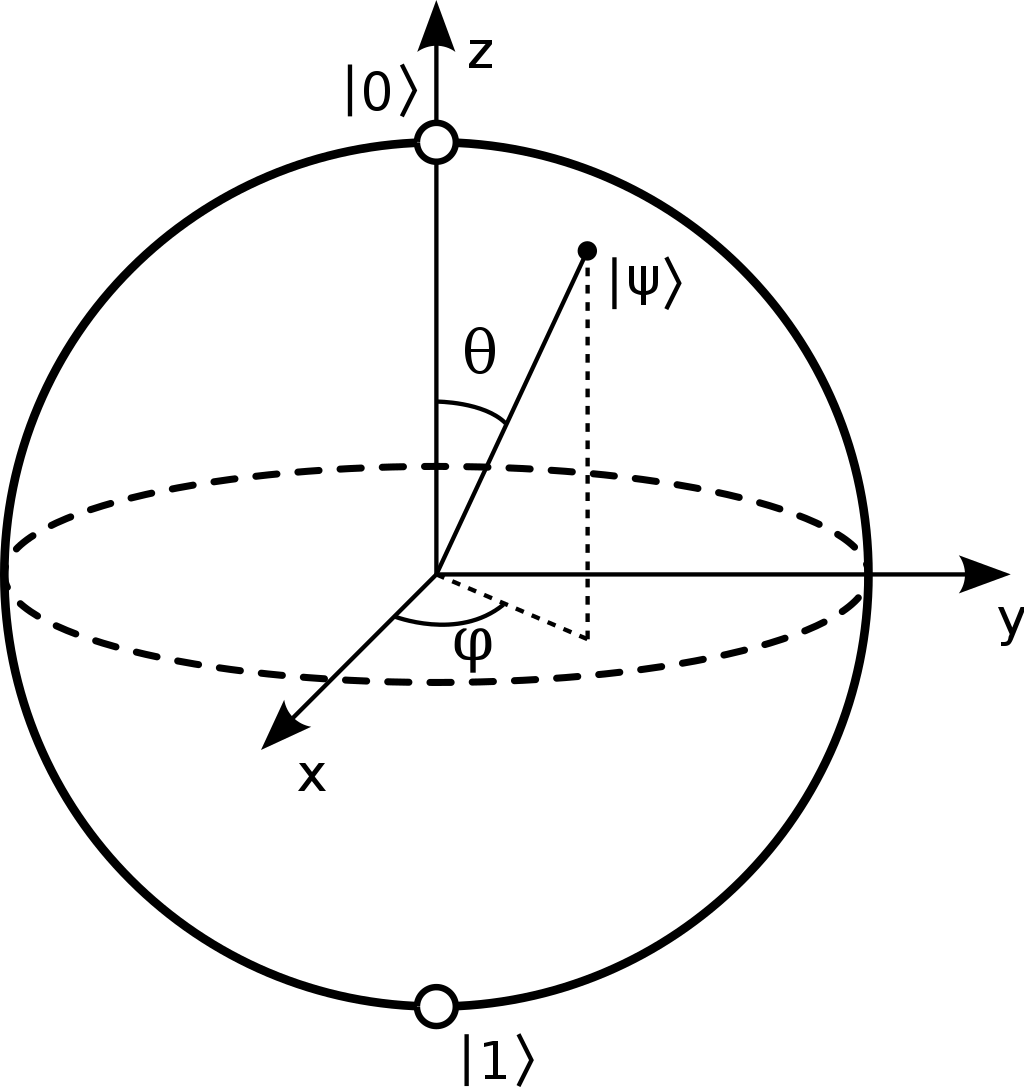
\includegraphics[scale=0.2]{bloch_sphere_image.png}   
    \caption{Depiction of a qubit $\ket{\psi}$ on the Bloch sphere \cite{ref:bloch_pic}.}
    \label{fig:bloch_sphere}
\end{figure}

As $2x1$ complex-valued vectors, qubits can be ``multiplied" in several important ways. To explain them, we must first introduce the adjoint of a qubit. Given a qubit
\begin{align}
\ket{q}
=
\begin{pmatrix}
a \\ b
\end{pmatrix}
,\end{align}
its adjoint $\bra{q}$ is given by its Hermitian  conjugate 
\begin{align}
\bra{q}
=
\ket{q}^\dagger
=
\begin{pmatrix}
a^* & b^*
\end{pmatrix}
,\end{align}
where taking the Hermitian conjugate of an operator $A$ takes each of its elements from $a_{ij}$ to $a^*_{ji}$.

The inner-product of two qubits $\ket{q_1}$ and $\ket{q_2}$ is defined as
\begin{align}
\bra{q_1}\ket{q_2}
=
\begin{pmatrix} 
a^*_1 & b^*_1
\end{pmatrix}
\begin{pmatrix}
a_2 \\ b_2
\end{pmatrix}
=
a^*_1a_2+b^*_1b_2
.\end{align}
The outer-product of two qubits $\ket{q_1}$ and $\ket{q_2}$ is defined as
\begin{align}
\ket{q_1}\bra{q_2}
=
\begin{pmatrix} 
a_1 \\ b_1
\end{pmatrix}
\begin{pmatrix}
a^*_2 & b^*_2
\end{pmatrix}
=
\begin{pmatrix}
a_1a^*_2 & a_1b^*_2
\\
b_1a^*_2 & b_1b^*_2
\end{pmatrix}
.\end{align}
Finally, the tensor-product of two-qubits is defined as
\begin{align}
\ket{q_1q_2}
=
\ket{q_1}\otimes\ket{q_2}
=
\ket{00}&=\begin{pmatrix}
a_1 \\ b_1
\end{pmatrix}
\otimes
\begin{pmatrix}
a_2 \\ b_2
\end{pmatrix}
=\begin{pmatrix}
a_1\begin{pmatrix}
a_2 \\ b_2
\end{pmatrix}
\\
b_1\begin{pmatrix}
a_2 \\ b_2
\end{pmatrix}
\end{pmatrix}
=\begin{pmatrix}
a_1a_2 \\ a_1b_2 \\ b_1a_2 \\ b_1b_2
\end{pmatrix}
.\end{align}

\section{Quantum Gates}

\nocite{ref:qcqi}

Quantum gates are physical actions that are applied to the physical system representing the qubits. Mathematically, they are complex-valued, unitary matrices which act on the complex-values normalized vectors that represent qubits. As the quantum analog of classical logic gates (such as AND and OR), there is a corresponding quantum gate for every classical gate; however, there are quantum gates that have no classical counter-part. They act on a set of qubits and, changing their state. That is, if $U$ is a quantum gate and $\ket{q}$ is a qubit, then acting the gate $U$ on the qubit $\ket{q}$ transforms the qubit as follows:
\begin{align}
\ket{q}\overset{U}{\to}U\ket{q}
.\end{align}
This action would be represented as the following quantum circuit
\begin{align}
\label{simple_qc}
\Qcircuit
{
\lstick{\ket{q}} & \gate{U} & \rstick{U\ket{q}} \qw 
}
\end{align}
Quantum circuits are diagrammatic representations of quantum algorithms. The horizontal dimension corresponds to time; moving left to right corresponds to forward motion in time. They consist of a set of qubits $\ket{q_n}$ which are stacked vertically on the left-hand side of the diagram. Lines, called quantum wires, extend horizontally to the right from each qubit, representing its state moving forward in time. Additionally, they contain a set of quantum gates that are applied to the quantum wires. Gates are applied chronologically, left to right. With this, we can see that the quantum circuit above (\ref{simple_qc}) implies that the quantum gate $U$ is being applied to the qubit in state $\ket{q}$.

To explain what quantum circuits represent mathematically, consider the following circuit
\begin{align}
\label{simple_qc}
\Qcircuit @C=1em @R=1em
{
\lstick{\ket{q_0}} & \gate{A} & \gate{B} & \qw 
\\
\lstick{\ket{q_1}} & \gate{C} & \gate{D} & \qw 
}
\end{align}
This circuit implies the following mathematical statement
\begin{align}
\ket{q_0q_1}
&\to
(B\otimes D)(A\otimes C)\ket{q_0q_1}
\\
&\to
(BA)\otimes(DC)\ket{q_0q_1}
\\
&\to 
BA\ket{q_0}DC\ket{q_1}
.\end{align}
Note that the mathematical form is in reverse order from circuit form ($AB\leftrightarrow BA$). This is because the operator closest to the state (furthest to the right) acts first. Additionally, we are able to write the actions of the top two gates and the bottom two as acting separately on each qubit as every gate here is a single-qubit gate (acting on only one qubit). The same would not be true for certain two-qubit gates which would entangle the states of the two qubits, not allowing their state to be written in a separable form. Finally, we define the depth of a quantum circuit as the number of columns of gates. The circuit above thus has a depth of 2 because it contains two columns of gates, namely $A\otimes C$ and $B\otimes D$.

\subsection{Single-Qubit Gates}

A single-qubit gate is a physical action that is applied to one qubit. It can be represented by a matrix $U$ from the group SU(2). Any single-qubit gate can be parameterized by three angles: $\theta$, $\phi$, and $\lambda$ as follows
\begin{align}
\label{U}
U(\theta,\phi,\lambda)
=
\begin{pmatrix}
\cos\frac{\theta}{2} & -e^{i\lambda}\sin\frac{\theta}{2}
\\
e^{i\phi}\sin\frac{\theta}{2} & e^{i(\phi+\lambda)}\cos\frac{\theta}{2}
\end{pmatrix}
.\end{align}
There are several widely used quantum gates, include the following:
The Pauli gates correspond to the Pauli matrices
\begin{align}
I
&=
\begin{pmatrix}
1 & 0 \\
0 & 1
\end{pmatrix}
\\
X
&=
\begin{pmatrix}
0 & 1 \\
1 & 0
\end{pmatrix}
\\
Y
&=
\begin{pmatrix}
0 & -i \\
i & 0
\end{pmatrix}
\\
Z
&=
\begin{pmatrix}
1 & 0 \\
0 & -1
\end{pmatrix}
,\end{align}
which satisfy the relation
\begin{align}
\comm{\sigma}{\tau}=i\epsilon_{\sigma\tau\upsilon}\upsilon
,\end{align}
for $\sigma,\tau,\upsilon\in\{X,Y,Z\}$. These gates form a basis for the algebra $\mathfrak{su}(2)$. Exponentiating them will thus give us a basis for SU(2), the group within which all single-qubit gates live. These exponentiated Pauli gates are called rotation gates $R_{\sigma}(\theta)$ because they rotate the quantum state around the axis $\sigma=X,Y,Z$ of the Bloch sphere (Figure \ref{fig:bloch_sphere}) by an angle $\theta$. They are defined as
\begin{align}
R_X(\theta)
&=
e^{-i\frac{\theta}{2}X}
=
\begin{pmatrix}
\cos\frac{\theta}{2} & -i\sin\frac{\theta}{2} \\
-i\sin\frac{\theta}{2} & \cos\frac{\theta}{2} 
\end{pmatrix},
\\
R_Y(\theta)
&=
e^{-i\frac{\theta}{2}Y}
=
\begin{pmatrix}
\cos\frac{\theta}{2} & -\sin\frac{\theta}{2} \\
\sin\frac{\theta}{2} & \cos\frac{\theta}{2} 
\end{pmatrix},
\\
R_Z(\theta)
&=
e^{-i\frac{\theta}{2}Z}
=
\begin{pmatrix}
e^{-i\theta/2} & 0 \\
0 & e^{i\theta/2}
\end{pmatrix}
.\end{align}
Because they form a basis for $\text{SU}(2)$, any single-qubit gate can be decomposed into three rotation gates. Indeed
\begin{align}
R_z(\phi)R_y(\theta)R_z(\lambda)
&=
\begin{pmatrix}
e^{-i\phi/2} & 0 \\
0 & e^{i\phi/2}
\end{pmatrix}
\begin{pmatrix}
\cos\frac{\theta}{2} & -\sin\frac{\theta}{2} \\
\sin\frac{\theta}{2} & \cos\frac{\theta}{2} 
\end{pmatrix}
\begin{pmatrix}
e^{-i\lambda/2} & 0 \\
0 & e^{i\lambda/2}
\end{pmatrix}
\\
&=
e^{-i(\phi+\lambda)/2}
\begin{pmatrix}
\cos\frac{\theta}{2} & -e^{i\lambda}\sin\frac{\theta}{2}
\\
e^{i\phi}\sin\frac{\theta}{2} & e^{i(\phi+\lambda)}\cos\frac{\theta}{2}
\end{pmatrix}
,\end{align}
which is, up to a global phase, equal to the expression for an arbitrary single-qubit gate (\ref{U}).

\subsection{Two-Qubit Gates}

A two-qubit gate is a physical action that is applied to two qubits. It can be represented by a matrix $U$ from the group SU(4). One important type of two-qubit gates are controlled gates, which work as follows: Suppose $U$ is a single-qubit gate. A controlled-$U$ gate ($CU$) acts on two qubits: a control qubit $\ket{x}$ and a target qubit $\ket{y}$. The controlled-$U$ gate applies the identity $I$ or the single-qubit gate $U$ to the target qubit if the control gate is in the zero state $\ket{0}$ or the one state $\ket{1}$, respectively. The control qubit is not acted upon. This can be represented as follows:
\begin{align}
CU\ket{xy}=
\begin{cases}
\ket{xy} & \text{if} \ \ket{x}=\ket{0}
\\
\ket{x}U\ket{y} & \text{if} \ \ket{x}=\ket{1}
\end{cases}
.\end{align}
The action of a controlled-$U$ gate $CU$ can be represented in a quantum circuit as follows
\begin{align}
\Qcircuit @C=1em @R=3em 
{
\lstick{\ket{x}} & \ctrl{1} & \rstick{\ket{x}} \qw
\\
\lstick{\ket{y}} & \gate{U} & \rstick{\begin{cases}\ket{y}, & \ket{x}=\ket{0} \\ U\ket{y}, & \ket{a}=\ket{x}\end{cases}} \qw
}
\\
\nonumber
\end{align}
It can be written in matrix form by writing it as a superposition of the two possible cases, each written as a simple tensor product
\begin{align}
CU 
&= \ket{0}\bra{0}\otimes I + \ket{1}\bra{1}\otimes U
\\
&=\begin{pmatrix}
1 & 0 & 0 & 0 \\
0 & 1 & 0 & 0 \\
0 & 0 & u_{00} & u_{01} \\
0 & 0 & u_{10} & u_{11}
\end{pmatrix}
.\end{align}
One of the most fundamental controlled gates is the CNOT gate. It is defined as the controlled-$X$ gate $CX$ and thus flips the state of the target qubit if the control qubit is in the zero state $\ket{0}$. It can be written in matrix form as follows:
\begin{align}
\text{CNOT}
=\begin{pmatrix}
1 & 0 & 0 & 0 \\
0 & 1 & 0 & 0 \\
0 & 0 & 0 & 1 \\
0 & 0 & 1 & 0
\end{pmatrix}
.\end{align}
A widely used two-qubit gate that goes beyond the simple controlled function is the SWAP gate. It swaps the states of the two qubits it acts upon
\begin{align}
\text{SWAP}\ket{xy}=\ket{yx}
,\end{align}
as depicted in the quantum circuit below
\begin{align}
\label{swap_def}
\Qcircuit
{
\lstick{\ket{x}} & \qswap      & \rstick{\ket{y}} \qw
\\
\lstick{\ket{y}} & \qswap \qwx & \rstick{\ket{x}} \qw
}
,\end{align}
and has the following matrix form
\begin{align}
\label{swap_def}
\text{SWAP}
=\begin{pmatrix}
1 & 0 & 0 & 0 \\
0 & 0 & 1 & 0 \\
0 & 1 & 0 & 0 \\
0 & 0 & 0 & 1
\end{pmatrix}
.\end{align}
It can be decomposed into a series of three CNOTs, each of which has its directionality flipped from the previous
\begin{align}
\Qcircuit
{
\lstick{\ket{x}} & \ctrl{1} & \targ     & \ctrl{1} & \rstick{\ket{y}} \qw
\\
\lstick{\ket{y}} & \targ    & \ctrl{-1} & \targ    & \rstick{\ket{x}} \qw
}
\end{align}
As for arbitrary two-qubit gates $U\in\text{SU(4)}$, they can be optimally decomposed (up to a global phase) into the following sequence \cite{ref:kak} involving three parameters, fifteen elementary one-qubit gates and three CNOT gates
\begin{align}
\Qcircuit
{
\qw & \gate{U_1} & \ctrl{1} & \gate{R_y(\theta_1)} & \targ      & \gate{R_y(\theta_2)} & \ctrl{1} & \gate{U_3} & \qw
\\
\qw & \gate{U_2} & \targ    & \gate{R_z(\theta_3)} & \ctrl{-1} & \qw                  & \targ     & \gate{U_4} & \qw
}
\end{align}
where $U_1,U_2,U_3,U_4$ are single-qubit gates, each of which can be decomposed into three elementary one-qubit gates (rotation gates). Additionally, $\theta_1,\theta_2,\theta_3$ are parameters to be determined by the arbitrary two-qubit gate to be decomposed. Two-qubit gates that are restricted to $U\in\text{SO(4)}$ can be decomposed into a shorter depth circuit consisting of just twelve elementary single-qubit gates and two CNOT gates
\begin{align}
\Qcircuit
{
\qw & \gate{R_z(\pi/2)} & \gate{R_y(\pi/2)} & \ctrl{1} & \gate{U_1} & \ctrl{1} & \gate{R^*_y(\pi/2)} & \gate{R^*_z(\pi/2)} & \qw
\\
\qw & \gate{R_z(\pi/2)} & \qw               & \targ    & \gate{U_2} & \targ    & \qw                 & \gate{R^*_z(\pi/2)} & \qw
}
\end{align}

\section{Variational Quantum Eigensolver}

\subsection{Introduction}

One initial algorithm to estimate the eigen-energies of a quantum Hamiltonian was quantum phase estimation \cite{ref:qpe}. In it, one encodes the eigen-energies, one binary bit at a time (up to $n$ bits), into the complex phases of the quantum states of the Hilbert space for $n$ qubits. It does this by applying powers of controlled unitary evolution operators to a quantum state that can be expanded in terms of the Hamiltonian's eigenvectors of interest. The eigen-energies are encoded into the complex phases in such a way that taking the inverse quantum Fourier transformation of the states into which the eigen-energies are encoded results in a measurement probability distribution that has peaks around the bit strings that represent a binary fraction which corresponds to the eigen-energies of the quantum state acted upon by the controlled unitary operators. While quantum phase estimation (QPE) is provably efficient, non-hybrid, and non-variational, the number of qubits and length of circuits required is too great for our NISQ era quantum computers. Thus, QPE is only efficiently applicable to large, fault-tolerant quantum computers that likely won't exist in the near, but the far future.

Therefore, a different algorithm for finding the eigen-energies of a quantum Hamiltonian was put forth in 2014 called the variational quantum eigensolver \cite{ref:vqe}, commonly referred to as VQE. The algorithm is hybrid, meaning that it requires the use of both a quantum computer and a classical computer. It is also variational, meaning that it relies, ultimately, on solving an optimization problem by varying parameters and thus is not as deterministic as QPE. The variational quantum eigensolver is based on the variational principle: The expectation value of a Hamiltonian $H$ in a state $|\psi(\theta)\rangle$ parameterized by a set of angles $\theta$, is always greater than or equal to the minimum eigen-energy $E_0$. To see this, let $|n\rangle$ be the eigenstates of $H$, that is:
\begin{align}
H|n\rangle=E_n|n\rangle
.\end{align}
We can then expand our state $|\psi(\theta)\rangle$ in terms of said eigenstates
\begin{align}
|\psi(\theta)\rangle=\sum_nc_n|n\rangle
,\end{align}
and plug this into the expectation value to yield
\begin{align}
\langle\psi(\theta)|H|\psi(\theta)\rangle
&=
\sum_{nm}c^*_mc_n\langle m|H|n \rangle
\nonumber
\\
&=
\sum_{nm}c^*_mc_nE_n\langle m|n \rangle
\nonumber
\\
&=
\sum_{nm}\delta_{nm}c^*_mc_nE_n
\nonumber
\\
&=
\sum_{n}|c_n|^2E_n
\nonumber
\\
&\geq
E_0\sum_{n}|c_n|^2
\nonumber
\\
&=
E_0
,\end{align}
which implies that we can minimize over the set of angles $\theta$ and arrive at the ground state energy $E_0$:
\begin{align}
\min_\theta \ \langle\psi(\theta)|H|\psi(\theta)\rangle
=
E_0
.\end{align}

\begin{figure}[h]
    \centering
    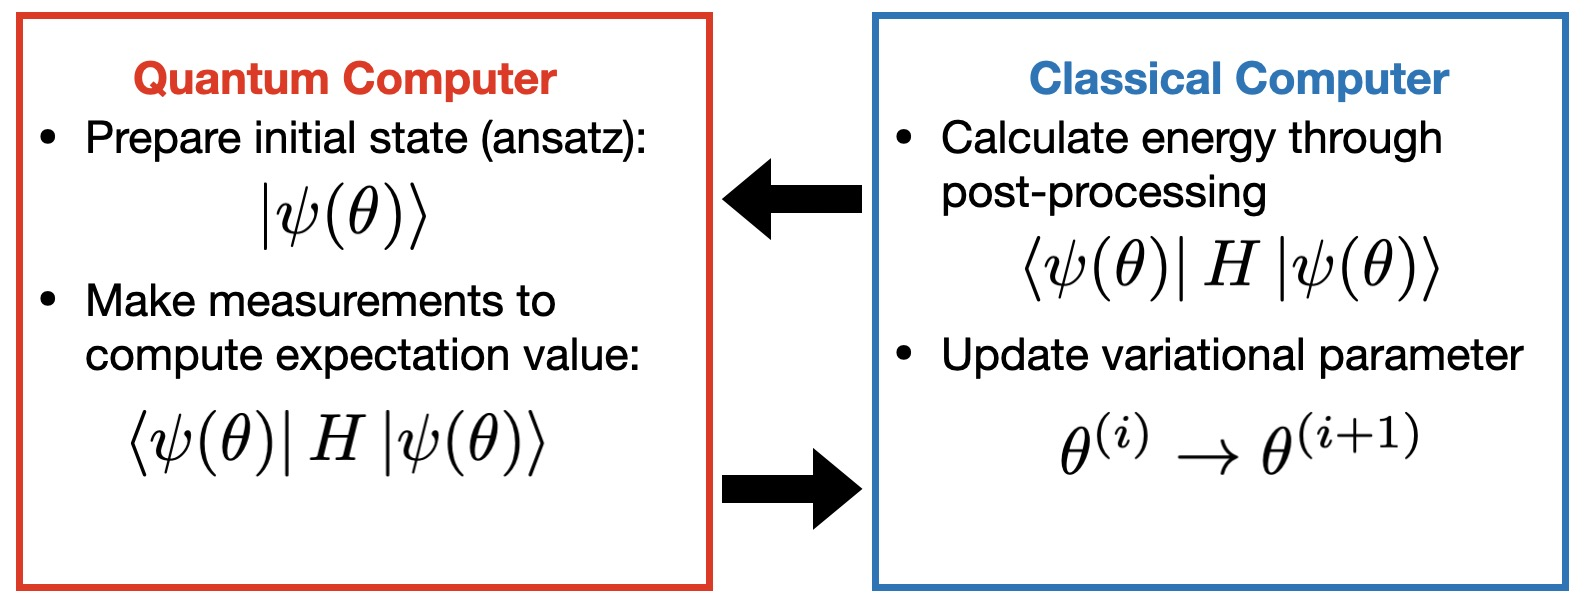
\includegraphics[scale=0.25]{vqe_schem.jpg}
    \caption{Schematic of the Variational Quantum Eigensolver}
    \label{fig:vqe_schem}
\end{figure}

Using this fact, the VQE algorithm can be broken down into the following steps, as noted in Figure \ref{fig:vqe_schem}:
\begin{enumerate}
    \item Prepare the variational state $|\psi(\theta)\rangle$ on a quantum computer.
    \item Measure this circuit in various bases and send these measurements to a classical computer
    \item The classical computer post-processes the measurement data to compute the expectation value $\langle\psi(\theta)|H|\psi(\theta)\rangle$
    \item The classical computer varies the parameters $\theta$ according to a classical minimization algorithm and sends them back to the quantum computer which runs step 1 again.
\end{enumerate}
This loop continues until the classical optimization algorithm terminates which results in a set of angles $\theta_{\text{min}}$ that characterize the ground state $|\phi(\theta_{\text{min}})\rangle$ and an estimate for the ground state energy $\langle\psi(\theta_{\text{min}})|H|\psi(\theta_{\text{min}})\rangle$.

\subsection{Expectation Values}
\label{expectation_values}

To execute the second step of VQE, we need to understand how expectation values of operators can be estimated via quantum computers by post-processing measurements of quantum circuits in different basis. To rotate bases, one uses the basis rotator $B_\sigma$ which is defined for each Pauli gate $\sigma$ to be
\begin{align}
B_{\sigma} =
\begin{cases}
H, & \text{if} \ \sigma = X \\
HS^{\dagger}, & \text{if} \ \sigma = Y \\
I, & \text{if} \ \sigma = Z \\
\end{cases}
.\end{align}
Note the following identity of the basis rotator
\begin{align}
B^\dagger_\sigma Z B_\sigma = \sigma
,\end{align}
which follows from the fact that $HZH=X$ and $SXS^\dagger=Y$. With this, we see that the expectation value of an arbitrary Puali-gate $\sigma$ in the state $\ket{\psi}$ can be expressed as a linear combination of probabilities
\begin{align}
E_{\psi}(\sigma)
&= \mel{\psi}{\sigma}{\psi} \nonumber \\
&=\mel{\psi}{B_{\sigma}^{\dagger}ZB_{\sigma}}{\psi} \nonumber \\
&=\mel{\phi}{Z}{\phi} \nonumber \\
&=\mel{\phi}{\left(\sum_{x\in\{0,1\}}(-1)^x\ket{x}\bra{x}\right)}{\phi} \nonumber \\
&=\sum_{x\in\{0,1\}}(-1)^x\abs{\bra{x}\ket{\phi}}^2\nonumber \\
&=\sum_{x\in\{0,1\}}(-1)^xP(\ket{\phi}\to\ket{x})
,\end{align}
where $\ket{\phi}=\ket{B_\sigma\phi}$ and $P(\ket{\phi}\to\ket{x}$ is the probability that the state $\ket{\phi}$ collapses to the state $\ket{x}$ when measured. This can be extended to any arbitrary Pauli string: consider the string of Pauli operators $P=\bigotimes_{p\in Q}\sigma_p$ which acts non-trivially on the set of qubits $Q$ which is a subset of the total set of $n$ qubits in the system. Then 
\begin{align}
E_{\psi}\left(P\right)
&=\bra{\psi}\left(\bigotimes_{p\in Q}\sigma_p\right)\ket{\psi} \nonumber \\
&=\bra{\psi}\left(\bigotimes_{p\in Q}\sigma_p\right)
\left(\bigotimes_{q\notin Q}I_q\right)\ket{\psi} \nonumber \\
&=\bra{\psi}\left(\bigotimes_{p \in Q}B_{\sigma_p}^{\dagger}Z_pB_{\sigma_p}\right)
\left(\bigotimes_{q\notin Q}I_q\right)\ket{\psi} \nonumber \\
&=
\bra{\psi}\left(\bigotimes_{p \in Q}B_{\sigma_p}^{\dagger}\right)
\left(\bigotimes_{p \in Q}Z_p\right)
\left(\bigotimes_{q\notin Q}I_q\right)
\left(\bigotimes_{p \in Q}B_{\sigma_p}\right)\ket{\psi} \nonumber 
\\
&=
\bra{\phi}
\left(\bigotimes_{p \in Q}Z_p\right)
\left(\bigotimes_{q\notin Q}I_q\right)
\ket{\phi} \nonumber \\
&=
\bra{\phi}
\left(\bigotimes_{p\in Q}\sum_{x_p\in\{0_p,1_p\}}(-1)^{x_p}\ket{x_p}\bra{x_p}\right)
\left(\bigotimes_{q\notin Q}\sum_{y_q\in\{0_q,1_q\}}\ket{y_q}\bra{y_q}\right)
\ket{\phi} 
\nonumber 
\\
&=
\bra{\phi}
\left(\sum_{x\in\{0,1\}^n}(-1)^{\sum_{p\in Q}x_p}\ket{x}\bra{x}\right)
\ket{\phi} 
\nonumber 
\\
&=
\sum_{x\in\{0,1\}^n}(-1)^{\sum_{p\in Q}x_p}\abs{\bra{x}\ket{\phi}}^2
\nonumber 
\\
&=
\sum_{x\in\{0,1\}^n}(-1)^{\sum_{p\in Q}x_p}P(\ket{\phi}\to\ket{x})
,\end{align}
where $\ket{\phi}=\ket{\bigotimes_{p\in Q}B_{\sigma_p}\psi}$. Finally, because the expectation value is linear
\begin{align}
E_\psi\left(\sum_{m}\lambda_mP_m\right) = \sum_m\lambda_mE_\psi(P_m)
,\end{align}
one can estimate any observable that can be written as a linear combination of Puali-string terms. 

\subsection{Measurement}

To estimate the probability $P(\ket{\phi}\to \ket{x})$ from the previous section, one prepares the state $\ket{\phi}$ on a quantum computer and measures it, and then repeats this process (prepare and measure) several times. The probability $P(\ket{\phi}\to \ket{x})$ is estimated to be the number of times that one measures the bit-string $x$ divided by the total number of measurements that one makes; that is
\begin{align}
\label{probability_approximation_definition}
P(\ket{\phi}\to \ket{x}) \approx \sum_{m=1}^M\frac{x_m}{M}
,\end{align}
where 
\begin{align}
x_m
=
\begin{cases}
1 & \text{if the result of measurement is $x$} 
\\
0 & \text{if the result of measurement is not $x$}.
\end{cases}
\end{align}
By the law of large numbers \cite{ref:lln}, the approximation (\ref{probability_approximation_definition}) approaches equality as $M$ goes to infinity
\begin{align}
\label{probability_approximation_definition}
P(\ket{\phi}\to \ket{x}) = \lim_{M\to\infty}\sum_{m=1}^M\frac{x_m}{M}
.\end{align}
As we obviously do not have infinite time nor infinite quantum computers (which could be run in parallel), we must truncate our number of measurement $M$ to a finite, but sufficiently large number. More precisely, for precision $\epsilon$, each expectation estimation subroutine within VQE requires $\mathcal{O}(1/\epsilon^2)$ samples from circuits with depth $\mathcal{O}(1)$ \cite{ref:precision}.

\section{Transformations}

While many-body nuclear physics operators are written in terms of fermionic operators, quantum computers work with Pauli operators. Thus, in order to simulate many-body nuclear physics on a quantum computer, we need a transformation between the two sets of operators. Several such transformations exist \cite{ref:transformations} (each with their own advantages and disadvantages) of which we list three here: Jordan-Wigner Parity-Basis, and Bravyi-Kitiav.

\begin{table}[h]
    \centering
    \begin{tabular}{c|c|c|c}
        Transformation & Basis & $\#$ of Operators & Locality \\
        \hline
        \hline
        Jordan-Wigner & Occupation Number & $\mathcal{O}(N)$ & Local \\
        \hline
        Parity-Basis & Parity & $\mathcal{O}(N)$ & Local \\
        \hline
        Bravyi-Kitiav & Mixed & $\mathcal{O}(\log(N))$ & Non-local
    \end{tabular}
    \caption{Comparison of basis, number of operators, and locality the of Jordan-Wigner, parity-basis, and Bravyi-Kitiav transformations.}
    \label{tab:transformation_comp}
\end{table}

Jordan-Wigner works in the occupation number representation which is naturally map-able to the computational basis set of a quantum computer, however it requires long strings of operators. Its main advantage for near-term devices is that it is local and hence implementable on linear-connectivity. The parity-basis transformation is similar to Jordan-Wigner except that it works in the parity-basis. The Bravyi-Kitiav transformation is a mix between the Jordan-Wigner and the parity-basis transformations that allows for a shorter number of operators but which comes with the cost of being non-local and hence not suitable for limited connectivity. In our work, we chose to use the Jordan-Wigner transformation because, although it requires more operators ($\mathcal{O}(N)$) it uses the occupation number representation, which is naturally implementable on a quantum computer. Additionally, it is local, making it more easily implementable on devices with limited qubit connectivity which describes most near-term devices. Here, qubit connectivity refers to which qubits are connected to which other qubits. Two qubits are connected if one can implement a two-qubit gate between them.

\subsection{Jordan-Wigner Transformation}

The Jordan-Wigner transformation was originally developed by Pascual Jordan and Eugene Wigner for one-dimensional lattice models \cite{ref:jwt}. The transformation is a mapping between fermionic and Pauli operators which stores information locally in the occupation number basis. It is given below as
\begin{align}
\label{jwt}
a^\dagger_p&=\left(\prod_{n=1}^{p-1}Z_n\right)Q^-_p,
\\
a_p&=\left(\prod_{n=1}^{p-1}Z_n\right)Q^+_p
,\end{align}
where
\begin{align}
Q^{\pm}_p
=
\frac{X_p \pm i Y_p}{2}
,\end{align}
and
\begin{align}
P_p = \left(\bigotimes_{n=1}^{p-1}I\right)\otimes P \otimes \left(\bigotimes_{n=p+1}^{N}I\right)
,\end{align}
where $P=I,X,Y,Z$ is a Pauli operator and $N$ is the size of the system (number of qubits). To gain some intuition for the mapping, note that the action on many-fermionic states (\ref{fermionic_op_on_states_def}) is preserved
\begin{align}
\dagg{a_i}\ket{n_1\ldots n_n}
&=
\left(\prod_{n=1}^{p-1}Z_n\right)Q^-_p\ket{n_1\ldots n_n}
=
(-1)^{N_p}(1-n_p)\ket{n_1\ldots n_{p-1}1n_{p+1}\ldots n_n},
\\
a_i\ket{n_1\ldots n_n}
&=
\left(\prod_{n=1}^{p-1}Z_n\right)Q^+_p\ket{n_1\ldots n_n}
=
(-1)^{N_p}n_p\ket{n_1\ldots n_{p-1}0n_{p+1}\ldots n_n},
\end{align}
where $N_p=\sum_{m=1}^{p-1}n_m$, since
\begin{align}
Z\ket{n}&=(-1)^n\ket{n},
\\
Q^-\ket{n}&=(1-n)\ket{1},
\\
Q^+\ket{n}&=n\ket{0},
\end{align}
where $n=0,1$. The mapping holds because it obeys the fermionic anti-commutation relations (\ref{fermionic_anticommutation_relations}) as verified below: First, consider the case $p=q$. In this case, the anti-commutation relations are
\begin{align}
\acomm*{a_p}{a^\dagger_p}
&=
\acomm{\left(\prod_{n=1}^{p-1}Z_n\right)Q^+_p}{\left(\prod_{n=1}^{p-1}Z_n\right)Q^-_p}
=
\left(\prod_{n=1}^{p-1}\acomm{Z_n}{Z_n}\right)
\acomm*{Q^+_p}{Q^-_p}
=
I_p
\\
\acomm*{a_p}{a_p}
&=
\acomm{\left(\prod_{n=1}^{p-1}Z_n\right)Q^+_p}{\left(\prod_{n=1}^{p-1}Z_n\right)Q^+_p}
=
\left(\prod_{n=1}^{p-1}\acomm{Z_n}{Z_n}\right)
\acomm*{Q^+_p}{Q^+_p}
=
0
\\
\acomm*{a^\dagger_p}{a^\dagger_p}
&=
\acomm{\left(\prod_{n=1}^{p-1}Z_n\right)Q^-_p}{\left(\prod_{n=1}^{p-1}Z_n\right)Q^-_p}
=
\left(\prod_{n=1}^{p-1}\acomm{Z_n}{Z_n}\right)
\acomm*{Q^-_p}{Q^-_p}
=
0,
\end{align}
which follow from the fact that
\begin{align}
\acomm*{Q^{\pm}_p}{Q^{\mp}_p}
&=
\frac{1}{4}\acomm*{X_p \pm iY_p}{X_p \mp iY_p}
\nonumber
\\
&=
\frac{1}{4}(\acomm*{X_p}{X_p} \mp i\acomm*{X_p}{Y_p} \pm i\acomm*{Y_p}{X_p}+\acomm*{Y_p}{Y_p})
=I_p
,\end{align}
while
\begin{align}
\acomm*{Q^{\pm}_p}{Q^{\pm}_p}
&=
\frac{1}{4}\acomm*{X_p \pm iY_p}{X_p \pm iY_p}
\nonumber
\\
&=
\frac{1}{4}(\acomm*{X_p}{X_p} \pm i\acomm*{X_p}{Y_p} \pm i\acomm*{Y_p}{X_p}-\acomm*{Y_p}{Y_p})
=0
.\end{align}
Second, consider the case $p\neq q$. Without loss of generality, we can set $p<q$. In this case, the anti-commutation relations are
\begin{align}
\acomm*{a_p}{a^\dagger_q}
&=
\acomm{\left(\prod_{n=1}^{p-1}Z_n\right)Q^+_p}{\left(\prod_{n=1}^{q-1}Z_n\right)Q^-_p}
\\
&=
\left(\prod_{n=1}^{p-1}\acomm{Z_n}{Z_n}\right)
\acomm*{Q^+_p}{Z^-_p}
\left(\prod_{m=p+1}^{q-1}\acomm{I_n}{Z_m}\right)
\acomm*{I_q}{Q^-_q}
=
0
\\
\acomm*{a_p}{a_q}
&=
\acomm{\left(\prod_{n=1}^{p-1}Z_n\right)Q^+_p}{\left(\prod_{n=1}^{q-1}Z_n\right)Q^+_p}
\\
&=
\left(\prod_{n=1}^{p-1}\acomm{Z_n}{Z_n}\right)
\acomm*{Q^+_p}{Z^-_p}
\left(\prod_{m=p+1}^{q-1}\acomm{I_n}{Z_m}\right)
\acomm*{I_q}{Q^+_q}
=
0
\end{align}
\begin{align}
\acomm*{a^\dagger_p}{a^\dagger_q}
&=
\acomm{\left(\prod_{n=1}^{p-1}Z_n\right)Q^-_p}{\left(\prod_{n=1}^{q-1}Z_n\right)Q^-_p}
\\
&=
\left(\prod_{n=1}^{p-1}\acomm{Z_n}{Z_n}\right)
\acomm*{Q^-_p}{Z^-_p}
\left(\prod_{m=p+1}^{q-1}\acomm{I_n}{Z_m}\right)
\acomm*{I_q}{Q^-_q}
=
0
,\end{align}
which follow from the fact that
\begin{align}
\acomm{Q^{\pm}_p}{Z_p}=\frac{1}{2}\acomm{X \mp iY}{Z}
=\frac{1}{2}\left(\acomm{X}{Z}\mp i\acomm{Y}{Z}\right)=0
\end{align}

\subsection{Pair Jordan-Wigner Transformation}

The Jordan-Wigner transformation is simplified when dealing with pair fermionic operators:
\begin{align}
A^\dagger_p&=Q^-_p,
\\
A_p&=Q^+_p,
\\
N_p&=1-Z_p
.\end{align}
Namely, the string of $Z$ operators preceding the $Q^\pm$ operator is dropped. This is one of the main advantages of working with the nuclear pairing model. Because it can be written in terms of pair fermionic operators, its mapping to quantum operators is greatly simplified. This mapping holds because it obeys the pair fermionic commutation relations (\ref{AAd_comm} - \ref{NA_comm}) as verified below:
\begin{align}
\comm*{A_p}{A^\dagger_q}
&=
\comm*{Q^+_p}{Q^-_q}
\nonumber
\\
&=
\frac{1}{4}\comm*{X_p+iY_p}{X_q-iY_q}
\nonumber
\\
&=
\frac{1}{4}(\comm*{X_p}{X_q}-i\comm*{X_p}{Y_q}+i\comm*{Y_p}{X_q}+\comm*{Y_p}{Y_q})
\nonumber
\\
&=
\delta_{pq}Z_p
\nonumber
\\
&=
\delta_{pq}(1-N_p),
\end{align}
and
\begin{align}
\comm*{N_p}{A^\dagger_q}
&=
\comm*{I_p-Z_p}{Q^-_q}
\nonumber
\\
&=
\frac{1}{2}\comm*{I_p-Z_p}{X_q-iY_q}
\nonumber
\\
&=
\frac{1}{2}(\comm*{I_p}{X_q}-i\comm*{I_p}{Y_q}-\comm*{Z_p}{X_q}+i\comm*{Z_p}{Y_q})
\nonumber
\\
&=
\delta_{pq}\left(\frac{X_p-iY_p}{2}\right)
\nonumber
\\
&=
\delta_{pq}A^\dagger_p,
\end{align}
and
\begin{align}
\comm*{N_p}{A_q}
&=
\comm*{I_p-Z_p}{Q^+_q}
\nonumber
\\
&=
\frac{1}{2}\comm*{I_p-Z_p}{X_q+iY_q}
\nonumber
\\
&=
\frac{1}{2}(\comm*{I_p}{X_q}+i\comm*{I_p}{Y_q}-\comm*{Z_p}{X_q}-i\comm*{Z_p}{Y_q})
\nonumber
\\
&=
\delta_{pq}\left(\frac{X_p+iY_p}{2}\right)
\nonumber
\\
&=
\delta_{pq}A_p.
\end{align}

\chapter{Lipkin Model}
\label{chap:lipkin_model}

\section{Introduction}

The Lipkin model is an exactly solvable, many-body toy-model, first introduced in 1965 by Lipkin, Meschkov, and Glick \cite{ref:lipkin}. It is often used to test the validity of nuclear many-body methods. The version we consider here describes pairing interactions between two levels (with the same $j$-value that straddle the Fermi level). The model consists of $N$ nucleons, distributed over two, $\Omega$-degenerate levels which are indexed by $\sigma=\pm1$; here $\Omega=2j+1$. The model is depicted schematically in Figure \ref{fig:lipkin_schem} below. The solid lines represent the available energy levels while the dashed line represents the Fermi-level.
\begin{figure}[b]
    \centering
    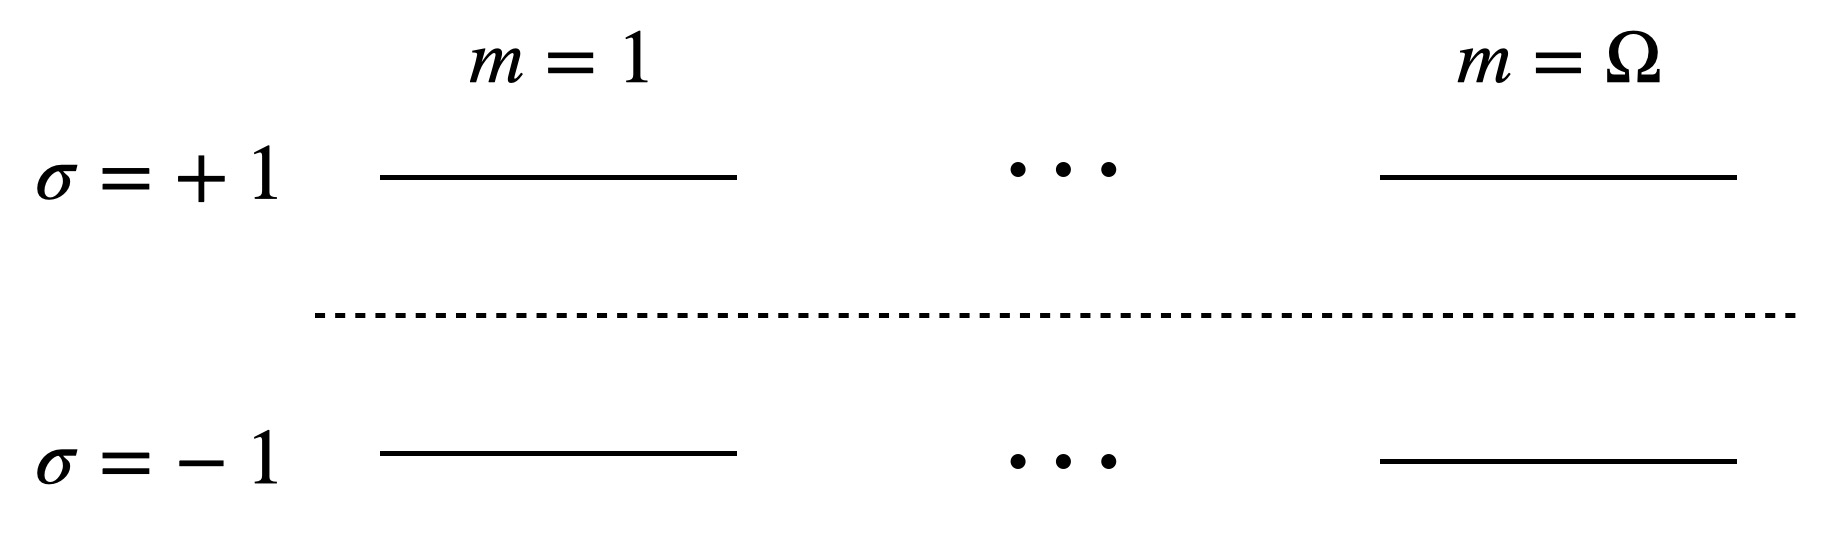
\includegraphics[scale=0.15]{Lipkin_Schematic.jpg}
    \caption{Schematic of Lipkin Model}
    \label{fig:lipkin_schem}
\end{figure}
The model is described by the following Hamiltonian
\begin{align}
\label{hamiltonian}
H
=
\frac{1}{2}\epsilon\sum_{n\sigma}\sigma a^\dagger_{n\sigma}a_{n\sigma}
-
\frac{1}{2}V
\sum_{nm\sigma}a^\dagger_{n\sigma}a^\dagger_{m\sigma}a_{m\bar{\sigma}}a_{n\bar{\sigma}}
,\end{align}
where $n,m=1,2,...,\Omega$ and $\sigma=\pm1$ (with $\bar{\sigma}=-\sigma$). The single-particle energy $\epsilon$ is the amount of energy required to move a nucleon between the lower-level ($\sigma=-1$) which has energy $-\epsilon/2$ to the upper-level ($\sigma=+1$) which has energy $\epsilon/2$. Additionally, the interaction strength $V$ is the energy required to move a pair of nucleons between the lower and upper levels. Note that in this model, nucleons must move between levels in pairs, either two in the lower level moving together to the upper or vice verse; this is why it is described as a pairing model.

\section{Classical Solutions}

\nocite{ref:lipkin_slide}

\subsection{Full Configuration Interaction}

The Lipkin model can be exactly solved via the full configuration interaction (FCI) method described in subsection (\ref{fci_subsection}). The FCI basis consists of the Slater determinants
\begin{align}
\ket{n}=\ket{n_1\cdots n_{2\Omega}}=(a^\dagger_1)^{n_1}...(a^\dagger_{2\Omega})^{n_{2\Omega}}\ket{0},
\end{align}
where $n_k=0,1$ is the occupation number of the state with index $m=\left \lfloor{k/2}\right \rfloor$ and $\sigma = 2[k \pmod2]-1$, for $k=1,2,...,2\Omega$. That is, even (odd) values of $k$ index the upper (lower) level, respectively. For $N$ nucleons, the FCI basis consists of all states $\ket{n}$ with a Hamming weight of $N$; that is, $n_k=1$ for $N$ values of $k$. The size of the basis is thus ${2\Omega \choose N}$. The diagonal Hamiltonian matrix elements are given by
\begin{align}
\mel{m_1\cdots m_{2\Omega}}{H}{n_1\cdots n_{2\Omega}}
=
\frac{\epsilon}{2}\left(N_+-N_-\right),
\end{align}
where $n_k=m_k$ for all $k$. Here
\begin{align}
N_+
&=
\sum_{k=0}^{\Omega-1}n_{2k+1},
\\
N_-
&=
\sum_{k=0}^{\Omega-1}n_{2k},
\end{align}
are the number of nucleons in the upper and lower levels, respectively. The off-diagonal matrix elements are given by
\begin{align}
\mel{m_1\cdots m_{2\Omega}}{H}{n_1\cdots n_{2\Omega}}
&=
-\frac{V}{2}
,\end{align}
where $n_{2k}n_{2j}n_{2k+1}n_{2j+1}=xx\bar{x}\bar{x}$ and $m_{2k}m_{2j}m_{2k+1}m_{2j+1}=\bar{x}\bar{x}xx$ for exactly one pair $(k,j)$ from $k\neq j=0,...,\Omega-1$, and $n_l=m_l$ for all $l\neq 2k,2k+1,2j,2j+1$. Here, $x=0,1$ with $\bar{0}=1$ and $\bar{1}=0$. The eigenvalues and eigenvectors are then found through direct diagonalization of the Hamiltonian matrix $H$ which has elements 
\begin{align}
H_{n_1\ldots n_{2\Omega},{n_1\ldots n_{2\Omega}}}=\mel{m_1\cdots m_{2\Omega}}{H}{n_1\cdots n_{2\Omega}}.   
\end{align}
The eigenvalue energies are computed for the case $\Omega=N=4$ against various values of the interaction strength $V$. They are depicted as the lines in Figure \ref{fig:fci_plot}. This was the largest value of $\Omega$ that could be solved in a reasonable amount of time on my laptop, underscoring the exponential time-scaling of the FCI method.

\begin{figure}[h]
    \centering
    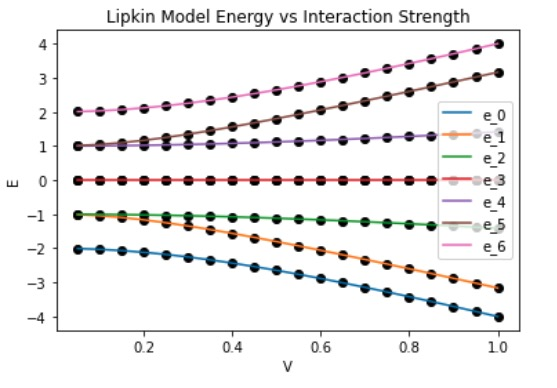
\includegraphics[scale=0.6]{fci_v_sym_lm.jpg}
    \caption{The energy eigenvalues ($E$) of the Lipkin model, are plotted for various interaction strengths ($V$). The level degeneracy $\Omega$ and particle number $N$ are both four while the single-particle energy $\epsilon$ is 1. The different energies $e_k$ for $k=0,1,...,6$ are depicted by different colors, labeled in the plot itself. The solid lines are the result of the FCI method while the black dots are the result of the symmetric method.}
    \label{fig:fci_plot}
\end{figure}

\subsection{Symmetry Method}
\label{subsection:symmetry_method}

Following the procedure of the symmetry method laid out in subsection (\ref{symmetry_method_subsection}), we start by identifying the symmetries of the Lipkin Hamiltonian. The first symmetry is the particle-number. The particle number operator
\begin{align}
N=\sum_{n\sigma}a^\dagger_{n\sigma}a_{n\sigma}
,\end{align}
commutes with the Lipkin Hamiltonian. This can be seen by examining the Hamiltonian (\ref{hamiltonian}) and noticing that the one-body part simply counts particles while the two-body term moves particles in pairs. Thus, the Hamiltonian conserves particle number. To find more symmetries we rewrite the Lipkin Hamiltonian in terms of SU(2) operators
\begin{align}
\label{lipkin_symmetry_hamiltonian}
H = \epsilon J_z + \frac{1}{2}V(J^2_++J^2_-),
\end{align}
via the mapping
\begin{align}
\label{jz}
J_z
&=
\sum_{n}j_z^{(n)},
\\
\label{jpm}
J_\pm&=\sum_nj^{(n)}_{\pm},
\end{align}
where
\begin{align}
\label{small_jz}
j_z^{(n)}
&=
\frac{1}{2}\sum_{\sigma}\sigma a^\dagger_{n\sigma}a_{n\sigma},
\\
\label{small_jpm}
j^{(n)}_{\pm}
&=
a^\dagger_{n\pm}a_{n\mp}.
\end{align}
These operators obey the SU(2) commutation relations
\begin{align}
\label{comm1}
\comm{J_+}{J_-}&=2J_z,
\\
\label{comm2}
\comm{J_z}{J_\pm}&=\pm J_\pm,
\end{align}
as justified in Appendix \ref{appendix:angular_momentum_commutation_relations}. Here, the ladder operators are defined as $J_{\pm}= J_x\pm iJ_y$. With this rewriting, we can see that the total spin operator $J^2$, which is defined as 
\begin{align}
J^2= J^2_x+J^2_y+J^2_z =
\frac{1}{2}\acomm{J_+}{J_-}+J_z^2
,\end{align}
commutes with the Hamiltonian since the Hamiltonian is written explicitly in terms of SU(2) operators and $J^2$ is the center of SU(2), meaning that it commutes with all of its elements. Finally, we note that the signature operator
\begin{align}
R=e^{i\phi J_z}
,\end{align}
commutes with the Hamiltonian, which can be explained as follows: Writing $J_z$ as
\begin{align}
J_z=\frac{1}{2}(N_+-N_-),
\end{align}
where $N_\pm=\sum_{n\pm}a^\dagger_{n\pm}a_{n\pm}$, allows us to see that it measures half the difference between the number of particles in the upper and lower levels. Thus, the possible eigenvalues $r$ of the signature operator are
\begin{align}
r
=
\begin{cases}
+1, & j_z=2n \\
+i, & j_z=2n+\frac{1}{2} \\
-1, & j_z=2n+1 \\
-i, & j_z=2n+\frac{3}{2} \\
\end{cases}
\end{align}
for $n\in\mathbb{Z}$. Note that $r$ is real or imaginary if the number of particles $N$ is even or odd, respectively. Since, as discussed above, the Lipkin Hamiltonian conserves $N$, $r$ cannot jump between being real and imaginary. Additionally, because particles must be moved in pairs, and $J_z$ measures half the difference between particles in the upper and lower levels, $j_z$ can only change by as
\begin{align}
j_z
&\to
\frac{1}{2}[(N_+\pm 2n)-(N_-\mp 2n)]
\nonumber
\\
&=
J_z\pm2n.
\end{align}
We have determined that the symmetry operators $N$, $J$, and $R$ commute with the Hamiltonian. Let their eigenvalues be $n$, $j$, and $r$, respectively. These become our new quantum numbers. Starting with the particle number operator $N$, because $H$ cannot mix states from one particle number to another $\mel{N}{H}{N'}=0$ if $N\neq N'$, where $\ket{N}$ represents a state with $n$ particles,
the Hamiltonian matrix is block diagonal with $N$ blocks. Each block corresponds to a different particle number ($n=0,1,...,2\Omega$) with size $n^2/4+n$. This is a direct result of the particle number symmetry. We now move on to the total-spin operator. Because the Hamiltonian can not mix states with different $J$, we have that $\mel{J}{H}{J'}=0$ for $J\neq J'$. Now, for a given $N$, we label our basis states $\ket{jj_z}$ where $j_z=-j,-j+1,...,j-1,j$.
The non-zero Hamiltonian matrix elements are
\begin{align}
\bra{JJ_z}H\ket{J'J'_z} 
&=
\delta_{JJ'}\epsilon j_z,
\\
\bra{JJ_z+2}H\ket{JJ_z} &= 
-\frac{V}{2}\sqrt{[j(j+1)-j_z(j_z+1)]}
\nonumber
\\
&\times
\sqrt{[j(j+1)-(j_z+1)(j_z+2)]},
\\
\bra{JJ_z-2}H\ket{JJ_z} &= 
-\frac{V}{2}\sqrt{[j(j+1)-j_z(j_z-1)]}
\nonumber
\\
&\times
\sqrt{[j(j+1)-(j_z-1)(j_z-2)]},
\end{align}
since the operators that make up the Hamiltonian act on the basis states as follows:
\begin{align}
J_z\ket{JJ_z}&=j_z\ket{JJ_z},
\\
J_{\pm}\ket{JJ_z}&=\sqrt{j(j+1)-j_z(j_z\pm1)}\ket{JJ_z\pm1}
,\end{align}
Note that the maximum possible value of $j_z$ is $N/2$ which would correspond to the state where all $N$ particles are spin up:
\begin{align}
j_z\ket{\uparrow\cdots\uparrow}
=
\frac{1}{2}\sum_{m\sigma}N_{m\sigma}\ket{\uparrow\cdots\uparrow}=\frac{N}{2}
.\end{align}
Therefore, the maximum value of $j$ is also $N/2$ and thus its possible values are $j=N/2,N/2-1,...,1$ if $N$ is even and $j=N/2,N/2-1,...,1/2$ if $N$ is odd. For each $j$ the possible values of $j_z$ are $j_z=j,j-1,...,-j$. Thus, there are $2j+1$ possible values of $j_z$ for each $j$. This implies that each $n$-block of the Hamiltonian matrix is itself a block diagonal matrix consisting of $\left\lfloor N/2 \right\rfloor$ blocks. Each block corresponds with a total spin value ($j=N/2,N/2-1,...$) and has length $2j+1$. This is the direct result of the total spin symmetry. Finally, we move to the signature $R$. Each $j$-block is again, itself a block diagonal with two blocks ($r=\pm1$ if $N$ is even or $r=\pm i$ if $N$ is odd) which have size $j$ and $j+1$, respectively. The energies are computed by direct diagonalization of the Hamiltonian matrix we've been describing above.

One can see in Figure \ref{fig:fci_plot} that the energies computed via the symmetry method (depicted as block dots) exactly match the results of the FCI method. This is a demonstration that the symmetry method is indeed a valid, exact solution for the Lipkin model. The symmetry method is also used to solve the Lipkin Hamiltonian for the case of $\Omega=N=10$. With the FCI method, this would involve diagonalizing a size ${20 \choose 10}\sim10^5$, square matrix. But, with the symmetry method, one need only diagonalize several smaller square matrices, the largest of which is size 30, which is $j(j+1)$ for $j=N/2$. The eigenvalues of the Lipkin Hamiltonian for single-particle energy $\epsilon=1$ are plotted against various pairing strengths $V$ in Figure \ref{fig:lipkin_energies}.

\begin{figure}
    \centering
    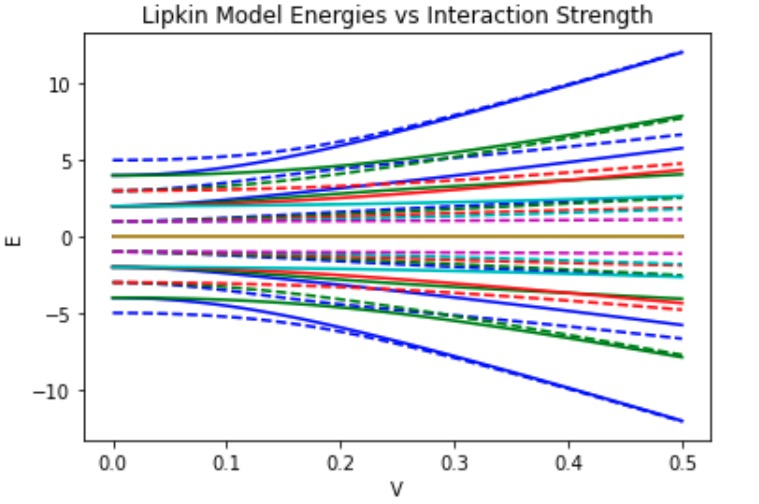
\includegraphics[scale=0.325]{lipkin_energies.jpg}
    \caption{The energy eigenvalues ($E$) of the Lipkin model, computed via the symmetry method, are plotted for various interaction strengths ($V$). The level degeneracy $\Omega$ and particle number $N$ are both ten while the single-particle energy $\epsilon$ is one. The solid and dashed lines correspond to signature numbers $r=+1$ and $r=-1$, respectively. The colors yellow, magenta, cyan, red, green, and blue correspond to $j$=0,1,2,3,4,5, respectively.}
    \label{fig:lipkin_energies}
\end{figure}
Each color represents a different value of $j$. For example, the eigenvalue energies plotted in blue were the result of diagonalizing the $j=5$ block. The lines are solid and dashed to correspond to the signature $r=+1$ and $r=-1$, respectively. We note that for $V=0$, there are $11=N+1$ values that the energies can take, corresponding to the fact that the Lipkin model with no interaction strength is simply $\epsilon J_z$; thus the Hamiltonian simply counts half the difference between the number of particles in the two levels, a number which has 11 possible values: $j_z=0,\pm1,\pm2,\pm3,\pm4,\pm5$. However, as the pairing strength is turned on, the energies start to bend and split. We notice that as $V$ increase, the energies for $r=+1$ and $r=-1$ start to pair up and equal one another, their states becoming degenerate. 

\subsection{Hartree-Fock Method}

As mentioned in subsection \ref{subsection:hartree_fock_theory}, the ansatz we use for the variational method is the particle-number conserving product state which, for the Lipkin model, is labeled as
\begin{align}
\ket{\tau}=\exp(\sum_{n}\tau_{n_+n_-}a^\dagger_{n+}a_{n-})\prod_{k=1}^Na^\dagger_k\ket{0},
\end{align}
where $\tau_{n_+n_-}$ is a variational parameter. This motivated by Thouless's theorem which states that such an ansatz can rotate any Slater determinant to any other. Since we are only considering single Slater determinants, this is exactly what we desire. Here, we consider the half-filled case $N=\Omega$. That is, the ansatz starts in the state
\begin{align}
\prod_{k=1}^Na^\dagger_k\ket{0}=\ket{J-J}
.\end{align}
However, because the Lipkin Hamiltonian treats all ($n+,n-$) pairs equivalently (the two-body coefficient $V$ is independent of $n$) we can set 
\begin{align}
\tau_{n_+n_-}=\tau,
\end{align}
a new variational parameter, for all $n$. With this, the normalized ansatz becomes
\begin{align}
\label{su2coh}
\ket{\tau}=(1+\abs{\tau}^2)^Je^{\tau J_+}\ket{0}
,\end{align}
where the normalization is determined in appendix \ref{appendix:normalization_of_the_hartree-fock_ansatz}. We now calculate the expectation value of the Hamiltonian in the ansatz. Using appendix \ref{appendix:lipkin_hamiltonian_matrix_elements_for_hf}, we derive
\begin{align}
\label{te}
\mel{\tau}{H}{\tau}
&=
\frac{\Omega}{2}\left[\epsilon\frac{\abs{\tau}^2-1}{\abs{\tau}^2+1}-V(\Omega-1)\frac{\tau^2+\bar{\tau}^2}{\left(\abs{\tau}^2+1\right)^2}\right],
\nonumber
\\
&=
-\frac{1}{2}\epsilon\Omega\left(\cos\theta+\frac{\chi}{2}\sin^2\theta\cos2\phi\right),
\end{align}
where we've defined the coupling strength $\chi$ to be
\begin{align}
\chi
=
\frac{V}{\epsilon}(\Omega-1).
\end{align}
This energy profile $E(\tau)=\mel{\tau}{H}{\tau}$ is plotted for various values of $\chi$ in Figure \ref{fig:butterfly}. The plot shows the symmetry breaking that occurs when $\chi$ becomes greater than 1. For $\chi\leq1$, there is only one $\theta_{\text{min}}$ (namely $\theta_{\text{min}}=0$). However, for $\chi>1$, there exist two values of $\theta_{\text{min}}$ which give the same, correct ground-state energy, and are symmetric about $\theta=0$.
\begin{figure}
    \centering
    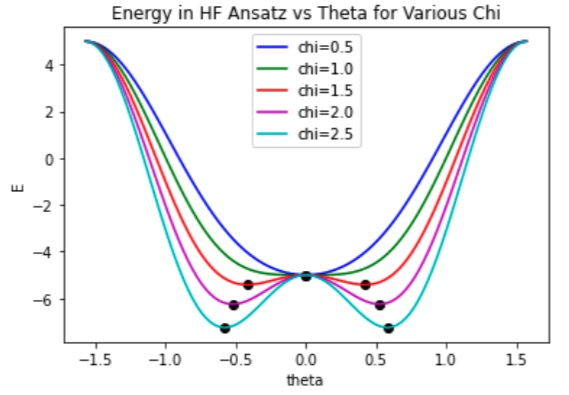
\includegraphics[scale=0.42]{butterfly.jpg}
    \caption{The expectation value of the Lipkin Hamiltonian in the SU(2) coherent state ansatz (\ref{su2coh}) is plotted vs theta for various values of $\chi$ which are distinguished by different colors, labeled on the plot itself. The black dots represent the minimum energy (\ref{theta_min}).}
    \label{fig:butterfly}
\end{figure}
To minimize $E(\tau)$, we first set its derivatives to zero:
\begin{align}
0
&=
\frac{\partial E}{\partial\theta}
=
\frac{1}{2}\epsilon\Omega\sin\theta(1-\chi\cos\theta\cos2\phi),
\\
0
&=
\frac{\partial E}{\partial\phi}
=
\frac{1}{2}\epsilon\Omega\chi\sin^2\theta\sin2\phi,
\end{align}
the first of which implies either $\theta_{\text{min}}=0,\pi$ or $\cos\theta_{\text{min}}\cos2\phi_{\text{min}}=1/\chi$ and the second of which implies either $\theta_{\text{min}}=0,\pi$ or $\phi_{\text{min}}=0,\pi/2$. Second, we demand that its second derivatives are positive
\begin{align}
0
&<
\frac{\partial^2E}{\partial\theta^2}
=\frac{1}{2}\epsilon\Omega(\cos\theta-\chi\cos2\theta\cos2\phi),
\\
0
&<
\frac{\partial^2E}{\partial\phi^2}
=
\epsilon\Omega\chi\sin^2\theta\cos2\phi
,\end{align}
which implies (assuming, without loss of generality, that $\chi>0$) that either $-\pi/3<\theta_{\text{min}}<\pi/3$, and $\phi_{\text{min}}<\pi/4$.
And third, we set the cross-derivative equal to zero
\begin{align}
0
=
\frac{\partial^2E}{\partial\theta\partial\phi}
=
\epsilon\Omega\chi\cos2\theta\sin2\phi
,\end{align}
which implies $\theta_{\text{min}}=0,\pi$. Combining all these conditions implies 
\begin{align}
\label{theta_min}
\theta_{\text{min}}
&=
\begin{cases}
0, & \text{if} \ 0<\chi\leq1
\\
\cos^{-1}\left(\frac{1}{\chi}\right), & \text{if} \ 1<\chi
\end{cases},
\\
\phi_{\text{min}}
&=0.
\end{align}
The minimum variational parameter is thus, $\tau_{\text{min}}=\tau(\theta_{\text{min}},\phi_{\text{min}})$ where $\tau(\theta,\phi)=\tan(\theta/2)e^{-i\phi}$, as defined in appendix \ref{appendix:lipkin_hamiltonian_matrix_elements_for_hf}. Finally, we plug the minimum $\theta$ back into $E(\tau)$ to find the ground state energy to be
\begin{align}
\label{e_hf}
E_0
&=
\begin{cases}
-\frac{\epsilon}{2}\Omega, & \text{if} \ 0<\chi<1
\\
-\frac{\epsilon}{4}\Omega\left(\chi+\frac{1}{\chi}\right), & \text{if} \ 1<\chi.
\end{cases}
\end{align}
The Hartree-Fock method is bench-marked against the exact answer in Figure \ref{fig:e0}. The Hartree-Fock calculated ground-state energy (\ref{e_hf}) is plotted against various values of the coupling strength $\chi$. Alongside it we plot the exact ground state energy computed using the symmetry method.
\begin{figure}
    \centering
    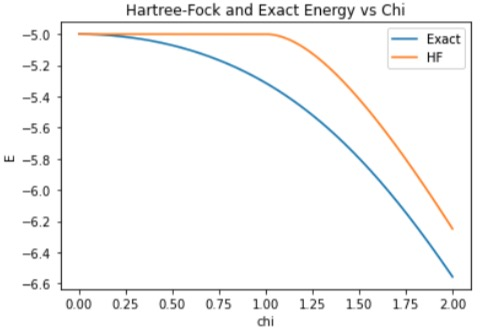
\includegraphics[scale=0.5]{HF_LM_plot.jpg}
    \caption{The Hartree-Fock and exact energy are plotted against various values of $\chi$.}
    \label{fig:e0}
\end{figure}
We more precisely inspect the performance of the Hartree-Fock method by plotting the relative error between the Hartree-Fock and exact energies in Figure \ref{fig:hfe}. We note that the two methods start in exact agreement at $\chi=0$. The magnitude of the relative error increases until just after 1. It then decreases as $\chi$ increases past 1 and seems to asymptotically approach a small error. Thus, one could say that the Hartree-Fock method is a good approximation for either very small $\chi$ or $\chi>2$.
\begin{figure}
    \centering
    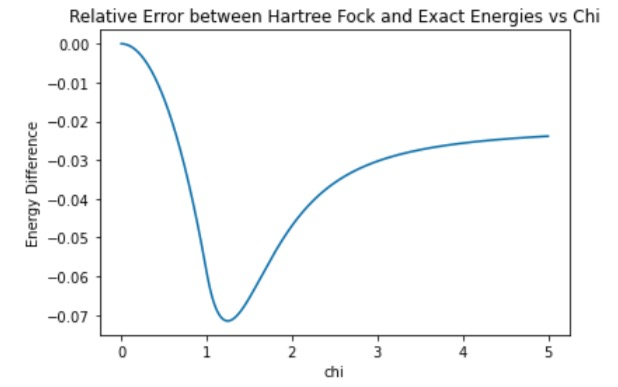
\includegraphics[scale=0.41]{HF_error.jpg}
    \caption{The relative difference between the Hartree-Fock and exact energies $(E_{\text{HF}}-E_{\text{exact}})/E_{\text{exact}})$ is plotted against various values of $\chi$.}
    \label{fig:hfe}
\end{figure}

\section{Quantum Solutions}

To solve the Lipkin model with a quantum computer, the first step is to map the system to a set of qubits. We'll restrict ourselves here to the half-filled case where the number of particles $N$ equals the degeneracy of the states $\Omega$. One could assign each possible state $(n,\sigma)$ a qubit such that the qubit being in the state $\ket{1}$ or $\ket{0}$ would imply that the state $(n,\sigma)$ is occupied or unoccupied, respectively. This mapping scheme (which we'll call occupation mapping) requires 2$\Omega$ qubits. Additionally, any ansatz that would restrict the minimization search to the correct subspace of constant Hamming weight $N$ (since the number of particles $N$ is conserved) would necessitate the use of at least four-qubit gates. This is because moving a pair of particles in this scheme would require two annihilation operators on the states from which the pair particles move and two creation operators on the states to which the pair of particles move. That is, it takes a four-qubit gate to change between the states $\ket{1100}$ and $\ket{0011}$, for example. And, as discussed in the chapter of quantum computing, it is only known how to efficiently decompose up to two qubit gates. Thus the involvement of four qubit gates would necessitate a longer depth circuit than one involving only two and one qubit gates, creating more noise and less accurate results.

However, because there are only two energy levels in the Lipkin model, any other natural mapping is possible. In this mapping scheme (which we'll call level mapping) each doublet ($(n,+1)$, $(n,-1)$) would be assigned a qubit such that the qubit being in the state $\ket{0}$ or $\ket{1}$ would imply that the particle is in the $(n,+1)$ or $(n,-1)$ state, respectively. Note that these are the only two possible configurations of the doublet as we are restricting ourselves to the half-filled case and the Lipkin Hamiltonian only moves particles between energy levels, not degenerate states. Thus the level mapping only requires $\Omega$ qubits which is half that of the occupation mapping. Additionally, any ansatz that would restrict the minimization search to the correct subspace of constant Hamming weight $N$ requires at most, only two qubit gates. This is because moving a pair of particles in this scheme only changes the state of two doublets (and therefore qubits). That is, it only takes a two-qubit gate to change between the states $\ket{00}$ and $\ket{11}$, for example. As an efficient decomposition two-qubit gates is known, the ansatz for this mapping would be shorter (and thus less noisy) than that of the previous mapping.

One could imagine a third mapping scheme which would require even less qubits in which each of the possible states in the spin basis $\ket{JJ_z}$ is mapped to a single qubit. In this spin mapping, there are only $2J+1$ possible states (since $J_z=-J,-J+1,...,J-1,J$) for each value of $J$. And, since the Hamiltonian is block diagonal (with a different block for each $J$) the eigenvalues of the Hamiltonian are simply the eigenvalues of each block, which may be calculated separately. Since the maximum value of $J$ is $J_{\text{max}}=N/2$, the largest number of qubits would be $2J_{\text{max}}+1=N+1$. However, $\left\lfloor N/2 \right\rfloor$ different circuit would need to be used for minimization for all possible values of $J$, to explore the entire Hilbert space. (The minimum of the set of minimum energies that each circuit finds would be the ground state energy of the entire system.) This increases, linearly, the amount of time required to find the ground state energy.

After reviewing the three possible mappings, it is our view that the level mapping \cite{ref:lipkin_naive} is the best suited for NISQ era devices given its low qubit count and ability to search the entire relevant Hilbert space with one circuit (which reduces time to solution) and the fact that at most, only two-qubit gates are required of the ansatz, leading to shorter depth (and thus less noisy) circuits. With this mapping, the Hamiltonian takes the form utilized in the symmetry method (subsection \ref{subsection:symmetry_method}) which was given by equation (\ref{lipkin_symmetry_hamiltonian}) as
\begin{align}
H
=
\epsilon J_z + \frac{1}{2}V(J^2_++J^2_-).
\end{align}
Plugging the mapping from the total $J$ operators to individual $j$ operators (equations \ref{small_jz} and \ref{small_jpm}) yields
\begin{align}
H
&=
\epsilon\sum_{n}j_z^{(n)} + \frac{1}{2}V\left[\left(\sum_nj^{(n)}_{+}\right)^2+\left(\sum_nj^{(n)}_{-}\right)^2\right]
\\
&=
\epsilon\sum_{n}j_z^{(n)} + \frac{1}{2}V\sum_{n,m}\left(j^{(n)}_+j^{(m)}_++j^{(n)}_-j^{(m)}_-\right)
\\
&=
\epsilon\sum_{n}j_z^{(n)} + 
2V\sum_{n<m}\left(j^{(n)}_xj^{(m)}_x-j^{(n)}_yj^{(m)}_y\right),
\end{align}
where we've used the definitions
\begin{align}
j_{\pm}^{(n)}=j_x^{(n)}\pm ij_y^{(n)}.
\end{align}
To convert to Pauli matrices, we'll make the transformations
\begin{align}
j_x^{(n)} &\to X_n/2,
\\
j_y^{(n)} &\to Y_n/2,
\\
j_z^{(n)} &\to Z_n/2,
\end{align}
which preserves the SU(2) commutation relations (\ref{comm1} and \ref{comm2}) and thus is allowable. This transforms our Hamiltonian into
\begin{align}
H=\frac{1}{2}\epsilon\sum_{k=1}^nZ_k+\frac{1}{2}V\sum_{n\neq j=1}^N(X_kX_j-Y_kY_j).
\end{align}
With this form, we can clearly see that the first (one-body) term in the Hamiltonian returns the energy $-\epsilon/2$ or $+\epsilon/2$ if the qubit representing the particle of a doublet is in the ground ($\ket{1}$) or excited ($\ket{0}$) state, respectively. The action of the second (two-body) term in the Hamiltonian can be determined by noting that
\begin{align}
\frac{1}{2}(XX-YY)\ket{00} &= \ket{11},
\\
\frac{1}{2}(XX-YY)\ket{01} &= 0,
\\
\frac{1}{2}(XX-YY)\ket{10} &= 0,
\\
\frac{1}{2}(XX-YY)\ket{11} &= \ket{00}.
\end{align}
That is, the two-body term moves a pair of particles between the ground states $\ket{00}$ and the excited states $\ket{11}$ of their respective doublets.  

To construct an efficient ansatz, we must determine the subspace within which the Hamiltonian lives. To begin, note that particles are only ever moved between energy levels in pairs. This implies that all possible states have a Hamming weight of constant parity (odd or even); this is the same as the signature $r$ being conserved. Further, note that the Hamiltonian's coefficients ($\epsilon$ and $V$) are state independent (do not depend on the indices $n$ or $m$) as the states labeled by these indices are degenerate and thus have the same energy level. Thus, the Hamiltonian treats all states with the same number of excited particles (Hamming weight of the state) as the same. Therefore, the following ansatz forms exactly cover the subspace within which the $N$-degenerate Hamiltonian explores:
\begin{align}
\ket{\psi_{\text{even}}}&=\sum_{k=0}^{\lfloor n/2 \rfloor}c_{2k}\ket{D^n_{2k}},
\\
\ket{\psi_{\text{odd}}}&=\sum_{k=0}^{\lfloor n/2 \rfloor}c_{2k+1}\ket{D^n_{2k+1}}.
\end{align}
Here $\ket{D^n_k}$ represents a Dicke state which is defined as equal superposition of all $n$-qubit states with Hamming weight $k$. That is
\begin{align}
\ket{D^n_k}
=
\frac{1}{\sqrt{{n \choose k}}}\sum_{x\in h^n_k}\ket{x},
\end{align}
where $h^n_k= \{\ket{x} \ | \ \text{l}(x) = n, \ \text{wt}(x) = k\}$. There are two ways we can think of to prepare such ansatz: The first is to prepare them exactly as it is known how to deterministically prepare Dicke states with linear depth. The reference provides an algorithm for preparing a set of gates $U^n_k$ that prepares a Dicke state from a product state of Hamming weight $k$; that is
\begin{align}
U^n_k\ket{1}^{\otimes k}\ket{0}^{\otimes n-k}=\ket{D^n_k}.
\end{align}
It then describes how to one can create an arbitrary superposition of Dicke states, which we modify here to restrict ourselves to a Hamming weight of constant parity. The circuit to construct such a state (for the $k=6$ case, as an example) is given below
\begin{align}
\label{dicke_superposition}
\Qcircuit @C=0.8em @R=0.8em
{
\lstick{\ket{0}} & \gate{R_y(\theta_0)} & \ctrl{1} & \qw & \qw & \qw & \qw & \gate{R_z{(\phi_0)}} & \multigate{5}{U^n_k} & \qw 
\\
\lstick{\ket{0}} & \qw & \targ & \ctrl{1} & \qw & \qw & \qw & \qw & \ghost{U^n_k} & \qw 
\\
\lstick{\ket{0}} & \qw & \qw & \gate{R_y{(\theta_1})} & \ctrl{1} & \qw & \qw & \gate{R_z{(\phi_1)}} & \ghost{U^n_k} & \qw
\\
\lstick{\ket{0}} & \qw & \qw & \qw & \targ & \ctrl{1} & \qw & \qw & \ghost{(U^n_k)} & \qw
\\
\lstick{\ket{0}} & \qw & \qw & \qw & \qw & \gate{R_y{(\theta_2})} & \ctrl{1} & \gate{R_z{(\phi_2})} & \ghost{U^n_k} & \qw
\\
\lstick{\ket{0}} & \qw & \qw & \qw & \qw & \qw & \targ & \qw & \ghost{U^n_k} & \qw
\
}
\end{align}
The $R_y$ gates and CNOT gates prepare an arbitrary real superposition of product states with even Hamming weight $k$; then the $R_z$ gates add arbitrary phases to each of the states
\begin{align}
\ket{000000}
\to \ &\cos(\theta_0/2)\ket{000000} 
\nonumber
\\
+\ &\sin(\theta_0/2)\cos(\theta_1/2)e^{i\theta_0}\ket{110000} 
\nonumber
\\
+\ &\sin(\theta_0/2)\sin(\theta_1/2)\cos(\theta_2/2)e^{i(\theta_0+\theta_1)}\ket{111100}
\nonumber
\\
+\ &\sin(\theta_0/2)\sin(\theta_1/2)\sin\theta_2/2)e^{i(\theta_0+\theta_1+\theta_2)}\ket{111111}.
\end{align}
Finally, $U^n_k$ converts each product state to its corresponding Dicke state. Thus, all together the circuit acts as
\begin{align}
\ket{000000}
\to \ &\cos(\theta_0/2)\ket{D^6_0} 
\nonumber
\\
+\ &\sin(\theta_0/2)\cos(\theta_1/2)e^{i\theta_0}\ket{D^6_2} 
\nonumber
\\
+\ &\sin(\theta_0/2)\sin(\theta_1/2)\cos(\theta_2/2)e^{i(\theta_0+\theta_1)}\ket{D^6_4}
\nonumber
\\
+\ &\sin(\theta_0/2)\sin(\theta_1/2)\sin\theta_2/2)e^{i(\theta_0+\theta_1+\theta_2)}\ket{D^6_6}.
\end{align}
The circuit (\ref{dicke_superposition}) can be extended naturally for any even value of $k$. For odd values of $k$, one need simply add a single-qubit to the top of the circuit for $k-1$ and apply the $X$ gate to it. Although this ansatz has linear depth, the circuit for $U^n_k$ involves several double-controlled gates which involve the usage of several CNOT gates to decompose. As the CNOT gate is often the noisiest gate in NISQ era quantum computers, it is best to minimize their use.

\section{Results}

In this section, we test out ansatz $\ref{dicke_superposition}$ for the Lipkin model with parameters. $\Omega =4$, $e=1$ and $v=1$. One can see if Figure \ref{fig:lipkin_vqe_plot} that running VQE with our ansatz matches the exact energy for the most part, and always performs better than Hartree-Fock. Because the simulations of VQE were noiseless, we hypothesize that the slight variations in some of the VQE dots (red) off of the exact energy line (blue) could be due to the minimization algorithm failing to converge properly. Finding as set of initial parameters that would initialize us to a state with a large overlap with the ground state would be beneficial.

\begin{figure}
    \centering
    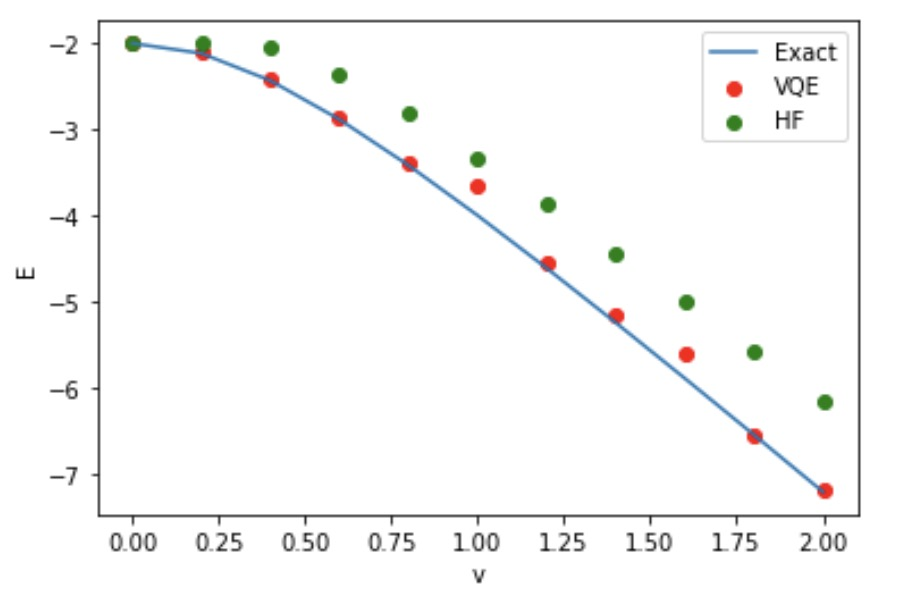
\includegraphics[scale=0.3]{lipkin_vqe_plot.jpg}
    \caption{Comparison of energies calculated through direct diagonalization (Exact), Hartree-Fock (HF) and the variational quantum eigensolver (VQE)}
    \label{fig:lipkin_vqe_plot}
\end{figure}

% Another way to construct this ansatz is through a variational "brick wall" layered ansatz; an example of which (for $k=4$) is given by the circuit below
% \begin{align}
% \label{brickwall}
% \Qcircuit
% {
% \lstick{\ket{0}}
% }
% \end{align}

% \subsection{Dicke State Reduction}
% \label{subsec:dicke_state_red}

\section{Conclusion} In this section, we introduced the Lipkin model which serves as a toy model in nuclear physics with which to benchmark new techniques. We first solve the problem through various classical avenues including via the full configuration interaction, the symmetry method, and the Hartree-Fock method. We then discussed the different ways to map the problem from its fermionic space to the spin space with which which quantum computers deal. We gave a novel way to construct one form of the ansatz for the model.

\chapter{Pairing Model}
\label{chap:pairing_model}

\section{Introduction}

The phenomenon of nuclear pairing can be understood from a simple symmetry argument. Since nucleons are fermions, the overall wavefunction of a pair nucleons must be anti-symmetric. Any such wavefunction can be written as the product of three separable wavefunctions: a spatial function, a spin function, and an isospin function. Pairing occurs between two fermions of opposite spin, which necessitates that the spin ($S=0$) function of their combined system be anti-symmetric. Additionally, pairing occurs most strongly between two nucleons of the same type (proton-proton or neutron-neutron) which is described by an isospin of $T=1$ which implies that the isospin function of their combined system is symmetric. The spin function being anti-symmetric and the isospin function being symmetric implies that the spatial function must be symmetric (to preserve the overall anti-symmetry of the pair). This occurs when the angular momentum component of the spatial wavefunction is zero $l=0$. This gives a wavefunction whose density has a strong peak near $r=0$ where $r$ is the separation between the two nucleons. Thus, the two nucleons tend to stick close together and can be approximated as a pair that moves together. Pairing occurs most strongly when $J=0$ because $J=S+L$ and we determined from above that $L=S=0$. Because of this, a large energy gap is produced between the $J=0$ and $J>0$ states by the nuclear force between identical nucleons. Therefore, one may approximate such a system via the so-called pairing interaction which only acts on the paired $J=0$ state \cite{ref:dean}. As we are approximating the residual interaction between identical nucleons, the pairing approximation is only suitable for semi-magic nuclei with valence nucleons of a single type \cite{ref:scholar}. This interaction was first introduced by Racah for atomic physics \cite{ref:racah}. The algebra of identical nucleon pairs (isospin $t=0$) is found to be isomorphic to SU(2) and is thus called quasi-spin. One of the earliest applications of pairing was by Bardeen, Cooper, and Schrieffer in their famous model (BCS) of superfluidity in condensed matter in 1957 \cite{ref:bcs}. The idea was adapted to pairing in nuclei by Bohr, Mottelson, and Pines in 1958 \cite{ref:bmp}.

\begin{figure}
    \centering
    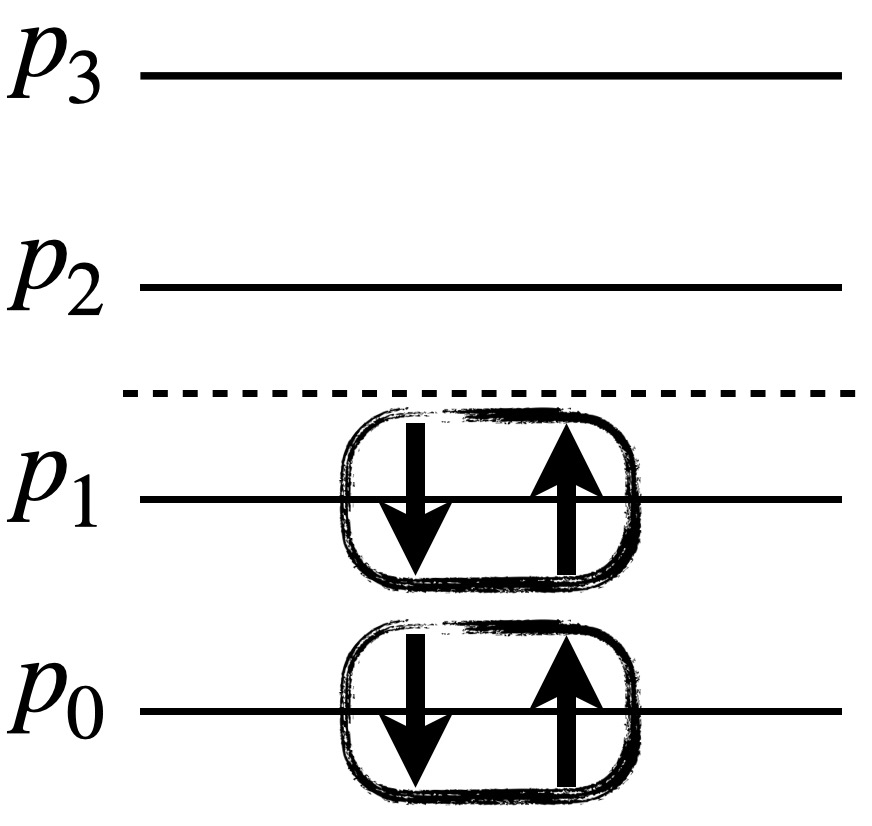
\includegraphics[width=0.25\textwidth]{pairing_schematic_pic.jpg}
    \caption{Example schematic of the paring model with $P=4$ and $N=2$. Shows four energy levels with single-particle energies $d_0,d_1,d_2,d_3$ of which the bottom two are initially filled by pairs. The dashed line represents the Fermi level which divides the energy levels with single-particle energies $d_0$ and $d_1$ (the hole states) from those with $d_2$ and $p_3$ (the particle states).}
    \label{fig:pairing_schem}
\end{figure}

In 1963, R.W. Richardson proposed a model consisting of fermions occupying non-degenerate energy levels which interact solely through the pairing force \cite{ref:rich1}-\cite{ref:rich2}. We refer here to his model as the pairing model. It consists of $P$, non-degenerate energy levels, occupied by $N$ pairs of fermions. Each pair consists of two fermions of opposite spin, occupying the same energy level. It's Hamiltonian is given by
\begin{align}
\label{pairing_model_hamiltonian_original}
H_p=\sum_{p\sigma}d_pa^\dagger_{p\sigma}a_{p\sigma}+\sum_{pq}g^p_qa^{\dagger}_{p+}a^{\dagger}_{p-}a_{q-}a_{q+}.
\end{align}
Here, the indices $p$ and $q$ sum over the set $\{0,...,P-1\}$, representing the different energy levels. Additionally, the index $\sigma$ sums over the set $\{-,+\}$, representing the spin of each fermion. The coefficients $d_p$ represent the single particle energies. For our analysis, we set the single particle energies to grow linearly with $d_p=p$. The coefficients $g^p_q$ are the so-called pairing strengths which represent the energy associated with moving a pair of fermions from the $q^{\text{th}}$ to the $p^{\text{th}}$ energy level. We will consider various sets of pairing strengths in this section. 

The pairing model can be rewritten in terms of so-called pairing operators as
\begin{align}
\label{pairing_model_hamiltonian}
H_p=\sum_{p=1}^nd_pN_p+\sum_{p,q=1}^ng^p_qA^\dagger_pA_q
.\end{align}
Here, $N_p$ is the pair number operator which counts the number of fermions occupying the $p^{\text{th}}$ energy level. Furthermore, $A^\dagger_p$ and $A_p$ are the pair fermionic creation and annihilation operators, respectively, which create and annihilate pairs of fermions on the $p^{\text{th}}$ energy level. These operators are defined in terms of fermionic creation and annihilation operators as follows
\begin{align}
\label{pair_fermionic_operators}
N_p &= \sum_{\sigma}a^\dagger_{p\sigma}a_{p\sigma}
\\
A^{\dagger}_p &= a^{\dagger}_{p+}a^{\dagger}_{p-}
\\
A_p &= a_{p-}a_{p+},
\end{align}
where $\sigma$, again, sums over the set $\{+,-\}$. The purpose of this rewriting becomes clear when one notices that these operators satisfy the $\text{SU}(2)$ algebra described by the following commutation relations
\begin{align}
\label{AAd_comm}
\comm*{A_p}{A^\dagger_q}&=\delta_{pq}(1-N_p),
\\
\label{NAd_comm}
\comm*{N_p}{A^\dagger_q}&=2\delta_{pq}A^\dagger_p,
\\
\label{NA_comm}
\comm*{N_p}{A_q}&=-2\delta_{pq}A_p.
\end{align}

\section{Classical Solutions}

\subsection{Exact Solution}

If one restricts the pairing strengths coefficients of the pairing model Hamiltonian (\ref{pairing_model_hamiltonian}) to be constant
\begin{align}
\label{pairing_model_hamiltonian_constant_g}
H=\sum_{p=1}^Pd_pN_p+g\sum_{p,q=1}^PA^\dagger_pA_q,
\end{align}
then there exists an exact solution, discovered by R.W. Richardson in 1963 \cite{ref:rich1}. The ansatz that solves the model with $N$ pairs is given by
\begin{align}
\label{richardson_ansatz}
\ket{\Psi}=\prod_{\alpha=1}^N B^\dagger_{\alpha}\ket{0},
\end{align}
where
\begin{align}
B^\dagger_\alpha=\sum_{\kappa=1}^P\frac{1}{2d_\kappa-E_\alpha}A^\dagger_\kappa,
\end{align}
which, when plugged into the Schrodinger equation leads to a set of equations (the Richardson equations) which we shall re-derive \cite{ref:rich_der} here. First, note that we can re-write the Schrodinger equation as
\begin{align}
\label{richardson_shcrodinger}
E\ket{\Psi}
&=
H\ket{\Psi}
\nonumber
\\
&=
H\prod_{\alpha=1}^NB^\dagger_{\alpha}\ket{0}
\nonumber
\\
&=
\comm*{H}{\prod_{\alpha=1}^NB^\dagger_{\alpha}}\ket{0},
\end{align}
since $H\ket{0}=0$. The commutator can be expanded as follows
\begin{align}
\label{expanded_commutator_HBd}
\comm*{H}{\prod_{\alpha=1}^N B^\dagger_{\alpha}}
=
\sum_{\alpha=1}^N
\left\{
\left(\prod_{\beta=1}^{\alpha-1}B^\dagger_\beta\right)
\comm*{H}{B^\dagger_\alpha}
\left(\prod_{\gamma=\alpha+1}^NB^\dagger_\gamma\right)
\right\},
\end{align}
the inner commutator of which is given by
\begin{align}
\comm*{H}{B^\dagger_\alpha}
&=
\comm*{\sum_{p=1}^Pd_pN_p+g\sum_{p,q=1}^PA^\dagger_pA_q}{\sum_{\kappa=1}^P\frac{1}{2d_\kappa-E_\alpha}A^\dagger_\kappa}
\\
&=
\sum_{\kappa=1}^P
\frac{1}{2d_\kappa-E_\alpha}
\left(
\sum_{p=1}^Pd_p\comm*{N_p}{A^\dagger_\kappa}
+
g\sum_{p,q=1}^P\comm*{A^\dagger_pA_q}{A^\dagger_\kappa}
\right)
\\
&=
\sum_{\kappa=1}^P
\frac{1}{2d_\kappa-E_\alpha}
\left(
\sum_{p=1}^P2\delta_{p\kappa}d_pA^\dagger_p
+
g\sum_{p,q=1}^P\delta_{q\kappa}A^\dagger_p(1-N_q)
\right)
\\
&=
\sum_{\kappa=1}^P
\frac{1}{2d_\kappa-E_\alpha}
\left(
2d_\kappa A^\dagger_\kappa
+
g\sum_{p=1}^PA^\dagger_p(1-N_\kappa)
\right)
\\
&=
\sum_{\kappa=1}^P
\left[
\left(\frac{E_\alpha}{2d_\kappa-E_\alpha}+1\right)
A^\dagger_\kappa
+
\frac{g}{2d_\kappa-E_\alpha}
\sum_{p=1}^PA^\dagger_p(1-N_\kappa)
\right]
\\
&=
E_\alpha B^\dagger_\alpha+\sum_{p=1}^PA^\dagger_p
\left(1+g\sum_{\kappa=1}^P\frac{1-N_\kappa}{2d_\kappa-E_\alpha}\right).
\end{align}
Plugging this back into the Schrodinger equation (\ref{richardson_shcrodinger}) and applying it to the vacuum yields
\begin{align}
E\ket{\Psi}
&=
\comm*{H}{\prod_{\alpha=1}^N B^\dagger_{\alpha}}\ket{0}
\nonumber
\\
&=
\sum_{\alpha=1}^N
\left\{
\left(\prod_{\beta=1}^{\alpha-1}B^\dagger_\beta\right)
\left[E_\alpha B^\dagger_\alpha+\sum_{p=1}^PA^\dagger_p
\left(1+g\sum_{\kappa=1}^P\frac{1-N_\kappa}{2d_\kappa-E_\alpha}\right)\right]
\left(\prod_{\gamma=\alpha+1}^NB^\dagger_\gamma\right)
\right\}
\ket{0}
\nonumber
\\
&=
E\ket{\Psi}
\nonumber
\\
&+
\sum_{\alpha=1}^N
\left\{
\left[
\left(1+\sum_{\kappa=1}^P\frac{g}{2d_\kappa-E_\alpha}\right)\sum_{p=1}^PA^\dagger_p
\right]
\left(\prod_{\beta=1,\beta\neq\alpha}^NB^\dagger_\beta\right)
\right\}
\ket{0}
\nonumber
\\
&-
\sum_{\alpha=1}^N
\left\{
\left(\prod_{\beta=1}^{\alpha-1}B^\dagger_\beta\right)
\left[
\left(
\sum_{\kappa=1}^P\frac{g}{2d_\kappa-E_\alpha}N_\kappa
\right)
\sum_{p=1}^PA^\dagger_p
\right]
\left(\prod_{\gamma=\alpha+1}^NB^\dagger_\gamma\right)
\right\}
\ket{0}
,\end{align}
where we've defined $E=\sum_{\alpha=1}^nE_\alpha$ and used the definition of $\ket{\Psi}$ (\ref{richardson_ansatz}) to simplify the first term, which implies that the Schrodinger equation is satisfied if
\begin{align}
\label{richardson_schrodinger_satisfied}
&\sum_{\alpha=1}^N
\left\{
\left(1+\sum_{\kappa=1}^P\frac{g}{2d_\kappa-E_\alpha}\right)
\prod_{\beta=1,\beta\neq\alpha}^NB^\dagger_\beta
\right\}
\ket{0}
\nonumber
\\
-&
\sum_{\alpha=1}^N
\left\{
\left(\prod_{\beta=1}^{\alpha-1}B^\dagger_\beta\right)
\left(
\sum_{\kappa=1}^P\frac{g}{2d_\kappa-E_\alpha}N_\kappa
\right)
\left(\prod_{\gamma=\alpha+1}^NB^\dagger_\gamma\right)
\right\}
\ket{0}
=0
,\end{align}
where we've divided through by the constant term $\sum_pA^\dagger_p$.
Note that the second term from above can be re-written as
\begin{align}
\label{second_term_richardson}
\sum_{\alpha=1}^N
\left\{
\left(\prod_{\beta=1}^{\alpha-1}B^\dagger_\beta\right)
\left(
\sum_{\kappa=1}^P\frac{g}{2d_\kappa-E_\alpha}
\right)
\comm*{N_\kappa}{\prod_{\gamma=\alpha+1}^NB^\dagger_\gamma}
\right\}
\ket{0}
,\end{align}
since $N_\kappa\ket{0}=0$. We'll now expand the commutator from the above expression
\begin{align}
\comm*{N_\kappa}{\prod_{\gamma=\alpha+1}^NB^\dagger_\gamma}
&=
\sum_{\gamma=\alpha+1}^N
\left\{
\left(\prod_{\mu=\alpha+1}^{\gamma-1} B^\dagger_\mu\right)
\comm*{N_\kappa}{B^\dagger_\gamma}
\left(\prod_{\nu=\gamma+1}^NB^\dagger_\nu\right)
\right\}
,\end{align}
the inner commutator of which is
\begin{align}
\comm*{N_\kappa}{B^\dagger_\gamma}
&=
\sum_{\lambda=1}^P\frac{1}{2d_\lambda-E_\gamma}
\comm*{N_\kappa}{A^\dagger_\lambda}
\\
&=
\sum_{\lambda=1}^P\frac{2}{2d_\lambda-E_\gamma}
\delta_{\kappa\lambda}A^\dagger_\kappa
\\
&=
\frac{2}{2d_\kappa-E_\gamma}
A^\dagger_\kappa.
\end{align}
Plugging this back into the second term (\ref{second_term_richardson}) yields
\begin{align}
\label{second_term_richardson3}
\sum_{\alpha=1}^N
\left\{
\left(\prod_{\beta=1}^{\alpha-1}B^\dagger_\beta\right)
\sum_{\gamma=\alpha+1}^N
\left\{
\left(\prod_{\mu=\alpha+1}^{\gamma-1} B^\dagger_\mu\right)
\left(
\sum_{\kappa=1}^P
\frac{2g}{(2d_\kappa-E_\alpha)(2d_\kappa-E_\gamma)}
A^\dagger_\kappa
\right)
\left(\prod_{\nu=\gamma+1}^NB^\dagger_\nu\right)
\right\}
\right\}
\ket{0}
.\end{align}
Applying partial fraction decomposition to the inner sum
\begin{align}
\frac{1}{(2d_\kappa-E_\alpha)(2d_\kappa-E_\gamma)}
=
\frac{1}{E_\alpha-E_\gamma}
\left(
\frac{1}{(2d_\kappa-E_\alpha)}
-
\frac{1}{(2d_\kappa-E_\gamma)}
\right)
,\end{align}
turns the second term (\ref{second_term_richardson3}) into
\begin{align}
\label{second_term_richardson2}
\sum_{\alpha=1}^N
\left\{
\left(\prod_{\beta=1}^{\alpha-1}B^\dagger_\beta\right)
\sum_{\gamma=\alpha+1}^N
\left\{
\left(\prod_{\mu=\alpha+1}^{\gamma-1} B^\dagger_\mu\right)
\left[
\frac{2g}{E_\alpha-E_\gamma}(B^\dagger_\alpha-B^\dagger_\gamma)
\right]
\left(\prod_{\nu=\gamma+1}^NB^\dagger_\nu\right)
\right\}
\right\}
\ket{0}
,\end{align}
which can be written as
\begin{align}
&\sum_{\alpha=1}^N
\sum_{\gamma=\alpha+1}^N
\left\{
\left(
\frac{2g}{E_\alpha-E_\gamma}
\right)
\left(\prod_{\beta=1,\beta\neq\gamma}^NB^\dagger_\nu\right)
\right\}
\ket{0}
\nonumber
\\
-&
\sum_{\alpha=1}^N
\sum_{\gamma=\alpha+1}^N
\left\{
\left(
\frac{2g}{E_\alpha-E_\gamma}
\right)
\left(\prod_{\beta=1,\beta\neq\alpha}^NB^\dagger_\nu\right)
\right\}
\ket{0}
.\end{align}
Switching the order of summation of the first term and swapping indices $\alpha\leftrightarrow\gamma$ followed by merging sums yields
\begin{align}
-&
\sum_{\alpha=1}^N
\sum_{\gamma=1}^{\alpha-1}
\left\{
\left(
\frac{2g}{E_\alpha-E_\gamma}
\right)
\left(\prod_{\beta=1,\beta\neq\alpha}^NB^\dagger_\nu\right)
\right\}
\ket{0}
\nonumber
\\
-&
\sum_{\alpha=1}^N
\sum_{\gamma=\alpha+1}^N
\left\{
\left(
\frac{2g}{E_\alpha-E_\gamma}
\right)
\left(\prod_{\beta=1,\beta\neq\alpha}^NB^\dagger_\nu\right)
\right\}
\ket{0}
\\
=-&
\sum_{\alpha=1}^N
\sum_{\gamma=1,\gamma\neq\alpha}^N
\left\{
\left(
\frac{2g}{E_\alpha-E_\gamma}
\right)
\left(\prod_{\beta=1,\beta\neq\alpha}^NB^\dagger_\nu\right)
\right\}
\ket{0}
.\end{align}
Finally, plugging this back into the condition that satisfies the Schrodinger equation (\ref{richardson_schrodinger_satisfied}) yields
\begin{align}
\sum_{\alpha=1}^N
\left\{
\left(
1
+
\sum_{\kappa=1}^P
\frac{g}{2d_\kappa-E_\alpha}
+
\sum_{\gamma=1,\gamma\neq\alpha}^N
\frac{2g}{E_\alpha-E_\gamma}
\right)
\left(
\prod_{\beta=1,\beta\neq\alpha}^NB^\dagger_\beta
\right)
\right\}
\ket{0}
=0
,\end{align}
which yields the Richardson equations
\begin{align}
\label{richardson_equations}
1
+
\sum_{\kappa=1}^P
\frac{g}{2d_\kappa-E_\alpha}
+
\sum_{\beta=1,\beta\neq\alpha}^N
\frac{2g}{E_\alpha-E_\beta}
=
0
,\end{align}
where we've relabeled $\gamma\to\beta$. This is a set of coupled, non-linear equations from which one solves for the terms $E_\alpha$ and sums them to find the energy; recall
\begin{align}
E=\sum_{\alpha=1}^N E_\alpha
.\end{align}
However, the Richardson equations are notoriously difficult to solve, due to the presence of singularities.

\subsection{Full Configuration Interaction}

The pairing model can be solved through exact diagonalization. In this method, the Hamiltonian is represented as a matrix with elements
\begin{align}
H_{p_ip_j,q_iq_j}
&=
\mel*{\Phi_{q_iq_j}}H{\Phi_{p_ip_j}}
\nonumber
\\
&=
\delta_{p_iq_i}\delta_{p_jq_j}[2(p_i+p_j)+g]
\nonumber
\\
&+
(\delta_{p_iq_i}(1-\delta_{p_jq_j})+(1-\delta_{p_iq_i})\delta_{p_jq_j})g
,\end{align}
where $\ket*{\Phi_{p_ip_j}}= a^\dagger_{p_i}a^\dagger_{p_j}\ket{0}$. Here, $i>j$ and $\ket{0}$ is the true vacuum. We've used the Hamiltonian written in terms of fermionic pair creation and annihilation operators (\ref{pairing_model_hamiltonian_original}). This Hamiltonian matrix is then diagonalized, its eigenvalues equal to the possible energies of the system.

\subsection{Many-body Perturbation Theory}
\label{subsection:mbpt}

The single particle energies $\epsilon_p$ (\ref{single_particle_energies}) for the pairing Hamiltonian are given by
\begin{align}
\epsilon_p 
&=
t^p_p+\sum_iv^{pi}_{pi}
\\
&=
d^p_p
+
\sum_{i}\delta_{pi}g^p_p
\\
&=
d^p_p
+
h(p)g^p_p
,\end{align}
and the interacting Hamiltonian $H_I$ is given by
\begin{align}
H_I
=
\sum_{p=1}^P(d_p-\epsilon_p)N_p+\sum_{p,q=1}^Pg^p_qA^\dagger_p A_q.
\end{align}
For the pairing model, the second and third order energy correlation contributions (\ref{final_delta_e2} - \ref{final_delta_e3}) are
\begin{align}
\label{pairing_delta_e2}
\Delta E^{(2)}
&=
\sum_{ai}\frac{g^a_ig^i_a}{\epsilon^{a}_{i}}
\nonumber
\\
&=
\frac{1}{2}\sum_{ai}\frac{g^a_ig^i_a}{d_i-d_a+g^i_i}
,\end{align}
and
\begin{align}
\label{pairing_delta_e3}
\Delta E^{(3)}
&=
\sum_{iab}
\frac{g^{i}_{b}g^{b}_{a}g^{a}_{i}}{\epsilon^{a}_{i}\epsilon^{b}_{i}}
+
\sum_{ija}
\frac{g^{a}_{j}g^{j}_{i}g^{i}_{a}}{\epsilon^{a}_{i}\epsilon^{a}_{j}}
\nonumber
\\
&=
\frac{1}{4}\sum_{iab}
\frac{g^{i}_{b}g^{b}_{a}g^{a}_{i}}{\left(d_i-d_a+g^i_i\right)\left(d_i-d_b+g^i_i\right)}
+
\sum_{ija}
\frac{g^{a}_{j}g^{j}_{i}g^{i}_{a}}{\left(d_i-d_a+g^i_i\right)\left(d_j-d_a+g^j_j\right)}
.\end{align}
One way to start with a good initial guess for $t$ is to compare the pCCD correlation energy (\ref{pccd_e_exp}) with the second order contribution to the correlation energy from MBPT (\ref{pairing_delta_e2})
\begin{align}
\sum_{ia}g^i_a{t^a_i}^{(0)}=\sum_{ia}g^i_a\frac{g^a_i}{\epsilon^{a}_{i}}
,\end{align}
which allows us to identify
\begin{align}
\label{t_init}
{t^a_i}^{(0)}
&=
\frac{g^a_i}{\epsilon^{a}_{i}}
\nonumber
\\
&=
\frac{1}{2}\frac{g^a_i}{d_i-d_a+g^i_i}
,\end{align}
for the pairing model. Many-body perturbation theory provides a more tractable, yet approximate, solution. The correlation energy from many-body perturbation theory, to second-order, is given by
\begin{align}
\Delta E_{\text{MBPT}2}
=
\sum_{ia}\frac{\abs{\mel{a}{v}{i}}^2}{\epsilon^a_i}
=\sum_{ia}\frac{1}{2}\frac{g^2}{i-a+g}
,\end{align}
since $\epsilon= \epsilon_i-\epsilon_a$ and
\begin{align}
\epsilon_p= h_{pp}+\sum_i\delta_{pi}\mel{p}{v}{p}
.\end{align}

\subsection{Pair CCD}

In this section, we apply the method of pair coupled cluster doubles theory (pCCD) to the above defined pairing model. The pair coupled cluster doubles equations (\ref{cc_energy} and \ref{cc_eq}) become
\begin{align}
\label{pccd_energy} 
E&=\mel{\Phi_0}{\overline{H}_p}{\Phi_0},
\\
\label{pccd_eq}
0&=\mel*{\Phi_i^a}{\overline{H}_p}{\Phi_0}
,\end{align}
where the similarity transformed pairing Hamiltonian is
\begin{align}
\overline{H}_p=e^{-T_p}H_pe^{T_p}
,\end{align}
which can be expanded via the BCH identity as
\begin{align}
\label{sim_H_p}
\overline{H}_p=H_p+\comm{H_p}{T_p}+\frac{1}{2}\comm{\comm{H_p}{T_p}}{T_p}+\cdots
.\end{align}
Though this expression is infinite, it can, in this case, be truncated to just the first three terms. This is because, when the expanded form of the similarity transformed pairing Hamiltonian (\ref{sim_H_p}) is inserted into the pCCD equations (\ref{pccd_energy} and \ref{pccd_eq}), one can truncate the resulting expressions by noting that only certain terms in the infinite sum (those which can be fully contracted) are non-zero. The truncated pCCD equations are
\begin{align}
\label{trunc_pccd_e}
E
&=
\bra*{\Phi}F_p+V_p+V_pT_p\ket{\Phi},
\\
\label{trunc_pccd_eq}
0
&=
\bra*{\Phi_i^a}V_p+F_pT_p+V_pT_p+\frac{1}{2}V_pT_p^2-T_pV_pT_p\ket{\Phi}
,\end{align}
where
\begin{align}
F_p
&=
\sum_pd_pN_p,
\\
V_p
&=
\sum_{pq}g^p_qA^\dagger_pA_q
,\end{align}
with the partitioning of the pairing model Hamiltonian a single-body and two-body term: $H_p=F_p+V_p$. We can save ourselves some work by recognizing that the first two terms of the truncated pCCD energy equation (\ref{trunc_pccd_eq}) equal the reference energy, and hence the pCCD correlation energy equation is
\begin{align}
\label{pccd_e_corr}
\Delta E = \mel{\Phi}{V_pT_p}{\Phi}
.\end{align}
Using Wick's theorem, we calculate the truncated pCCD energy equation (\ref{trunc_pccd_e})
\begin{align}
\mel{\Phi}{V_pT_p}{\Phi}
&=
\sum_{pqia}g_q^pt_i^a\mel{\Phi}{A^\dagger_pA_qA^\dagger_aA_i}{\Phi}
\nonumber
\\
&=
\sum_{pqia}g_q^pt_i^a\mel{\Phi}{
\contraction[1ex]{a^\dagger_{p+}a^\dagger_{p-}a_{q-}}{a}{_{q+}}
{a}
\contraction[2ex]{a^\dagger_{p+}a^\dagger_{p-}}{a}{_{q-}a_{q+}
a^\dagger_{a+}}{a}
\contraction[3ex]{a^\dagger_{p+}}{a}{^\dagger_{p-}a_{q-}a_{q+}
a^\dagger_{a+}a^\dagger_{a-}}{a}
\contraction[4ex]{}{a}{^\dagger_{p+}a^\dagger_{p-}a_{q-}a_{q+}
a^\dagger_{a+}a^\dagger_{a-}a_{i-}}{a}
a^\dagger_{p+}a^\dagger_{p-}a_{q-}a_{q+}
a^\dagger_{a+}a^\dagger_{a-}a_{i-}a_{i+}
}{\Phi}
\nonumber
\\
&=
\sum_{pqia}g_q^pt_i^a\delta_{pi}\delta_{qa}
\nonumber
\\
&=
\sum_{ia}g_a^it_i^a
.\end{align}
Turning our attention now to the truncated pCCD amplitude equation (\ref{trunc_pccd_e}), we start with
\begin{align}
\mel*{\Phi_i^a}{V_p}{\Phi}
&=
\sum_{pq}g_q^p\mel*{\Phi}{A^\dagger_iA_aA^\dagger_pA_q}{\Phi}
\nonumber
\\
&=
\sum_{pq}g_q^p\mel*{\Phi}{
\contraction[1ex]{a^\dagger_{i+}a^\dagger_{i-}a_{a-}}{a}{_{a+}}
{a}
\contraction[2ex]{a^\dagger_{i+}a^\dagger_{i-}}{a}{_{a-}a_{a+}
a^\dagger_{p+}}{a}
\contraction[3ex]{a^\dagger_{i+}}{a}{^\dagger_{i-}a_{a-}a_{a+}
a^\dagger_{p+}a^\dagger_{p-}}{a}
\contraction[4ex]{}{a}{^\dagger_{i+}a^\dagger_{i-}a_{a-}a_{a+}
a^\dagger_{p+}a^\dagger_{p-}a_{q-}}{a}
a^\dagger_{i+}a^\dagger_{i-}a_{a-}a_{a+}a^\dagger_{p+}a^\dagger_{p-}a_{q-}a_{q+}
}{\Phi}
\nonumber
\\
&=
\sum_{pq}g_q^p\delta_{pa}\delta_{qi}
\nonumber
\\
&=g_i^a
.\end{align}
To compute the next term $\mel*{\Phi_i^a}{F_pT_p}{\Phi}$, instead of writing out all possible contractions, it will be easier to compute the un-truncated term from which the this term comes, namely $\mel*{\Phi_i^a}{\comm*{F_p}{T_p}}{\Phi}$. We do so by using the commutation relations (\ref{NAd_comm} and \ref{NA_comm}) as follows
\begin{align}
\mel*{\Phi_i^a}{\comm*{F_p}{T_p}}{\Phi}
&=
\sum_{pjb}d_pt_j^b\bra*{\Phi_i^a}\comm*{N_p}{A^\dagger_bA_j}\ket{\Phi}
\nonumber
\\
&=
\sum_{pjb}d_pt_j^b\bra*{\Phi_i^a}(\comm*{N_p}{A^\dagger_b}A_j-A^\dagger_b\comm*{N_p}{A_j})\ket{\Phi}
\nonumber
\\
&=
2\sum_{pjb}d_pt_j^b(\delta_{pb}-\delta_{pj})\bra*{\Phi_i^a}A^\dagger_bA_j\ket{\Phi}
\nonumber
\\
&=
2\sum_{jb}(d_b-d_j)t_j^b\bra*{\Phi}A^\dagger_iA_aA^\dagger_bA_j\ket{\Phi}
\nonumber
\\
&=
2\sum_{jb}(d_b-d_j)t_j^b
\mel*{\Phi}{
\contraction[1ex]{a^\dagger_{i+}a^\dagger_{i-}a_{a-}}{a}{_{a+}}
{a}
\contraction[2ex]{a^\dagger_{i+}a^\dagger_{i-}}{a}{_{a-}a_{a+}
a^\dagger_{b+}}{a}
\contraction[3ex]{a^\dagger_{i+}}{a}{^\dagger_{i-}a_{a-}a_{a+}
a^\dagger_{b+}a^\dagger_{b-}}{a}
\contraction[4ex]{}{a}{^\dagger_{i+}a^\dagger_{i-}a_{a-}a_{a+}
a^\dagger_{b+}a^\dagger_{b-}a_{j-}}{a}
a^\dagger_{i+}a^\dagger_{i-}a_{a-}a_{a+}a^\dagger_{b+}a^\dagger_{b-}a_{j-}a_{j+}
}{\Phi}
\nonumber
\\
&=
2\sum_{jb}(d_b-d_j)t_j^b\delta_{ij}\delta_{ab}
\nonumber
\\
&=
2(d_a-d_i)t_i^a
.\end{align}
The same is true for the next term $\mel*{\Phi^a_i}{V_pT_p}{\Phi}$ and so it will be calculated analogously
\begin{align}
\mel*{\Phi^a_i}{\comm*{V_p}{T_p}}{\Phi}
&=
\sum_{pqjb}g^p_qt^b_j\mel*{\Phi^a_i}{\comm*{A^\dagger_pA_q}{A^\dagger_bA_j}}{\Phi}
\nonumber
\\
&=
\sum_{pqjb}g^p_qt^b_j\bra*{\Phi^a_i}(A^\dagger_pA^\dagger_b\cancel{\comm*{A_q}{A_j}}+A^\dagger_p\comm*{A_q}{A^\dagger_b}A_j
\nonumber
\\
&\hspace{28.75mm}+
A^\dagger_b\comm*{A^\dagger_p}{A_j}A_q+\cancel{\comm*{A^\dagger_p}{A^\dagger_b}}A_jA_q)\ket{\Phi}
\nonumber
\\
&=
\sum_{pqjb}g^p_qt^b_j\bra*{\Phi^a_i}(\delta_{qb}A^\dagger_p(1-N_b)A_j+\delta_{pj}A^\dagger_b(N_j-1)A_q)\ket{\Phi}
\nonumber
\\
&=
\sum_{pqjb}g^p_qt^b_j\bra*{\Phi^a_i}(\delta_{qb}A^\dagger_p(1-N_b)A_j+\delta_{pj}A^\dagger_bA_q(N_j-1)-2\delta_{pj}\delta_{qj}A^\dagger_bA_j)\ket{\Phi}
\nonumber
\\
&=
\sum_{jb}t^b_j\bra*{\Phi}A^\dagger_iA_a(g^p_bA^\dagger_pA_j+g^j_qA^\dagger_bA_q-2g^j_jA^\dagger_bA_j)\ket{\Phi}
\nonumber
\\
&=
\sum_{jb}t^b_j(g^p_b
\mel*{\Phi}{
\contraction[1ex]{a^\dagger_{i+}a^\dagger_{i-}a_{a-}}{a}{_{a+}}
{a}
\contraction[2ex]{a^\dagger_{i+}a^\dagger_{i-}}{a}{_{a-}a_{a+}
a^\dagger_{p+}}{a}
\contraction[3ex]{a^\dagger_{i+}}{a}{^\dagger_{i-}a_{a-}a_{a+}
a^\dagger_{p+}a^\dagger_{p-}}{a}
\contraction[4ex]{}{a}{^\dagger_{i+}a^\dagger_{i-}a_{a-}a_{a+}
a^\dagger_{p+}a^\dagger_{p-}a_{j-}}{a}
a^\dagger_{i+}a^\dagger_{i-}a_{a-}a_{a+}a^\dagger_{p+}a^\dagger_{p-}a_{j-}a_{j+}
}{\Phi}
\nonumber
\\
&\hspace{13mm}+
g^j_q
\mel*{\Phi}{
\contraction[1ex]{a^\dagger_{i+}a^\dagger_{i-}a_{a-}}{a}{_{a+}}
{a}
\contraction[2ex]{a^\dagger_{i+}a^\dagger_{i-}}{a}{_{a-}a_{a+}
a^\dagger_{b+}}{a}
\contraction[3ex]{a^\dagger_{i+}}{a}{^\dagger_{i-}a_{a-}a_{a+}
a^\dagger_{b+}a^\dagger_{b-}}{a}
\contraction[4ex]{}{a}{^\dagger_{i+}a^\dagger_{i-}a_{a-}a_{a+}
a^\dagger_{b+}a^\dagger_{b-}a_{q-}}{a}
a^\dagger_{i+}a^\dagger_{i-}a_{a-}a_{a+}a^\dagger_{b+}a^\dagger_{b-}a_{q-}a_{q+}
)}{\Phi}
\nonumber
\\
&\hspace{13mm}-2
g^j_j
\mel*{\Phi}{
\contraction[1ex]{a^\dagger_{i+}a^\dagger_{i-}a_{a-}}{a}{_{a+}}
{a}
\contraction[2ex]{a^\dagger_{i+}a^\dagger_{i-}}{a}{_{a-}a_{a+}
a^\dagger_{b+}}{a}
\contraction[3ex]{a^\dagger_{i+}}{a}{^\dagger_{i-}a_{a-}a_{a+}
a^\dagger_{b+}a^\dagger_{b-}}{a}
\contraction[4ex]{}{a}{^\dagger_{i+}a^\dagger_{i-}a_{a-}a_{a+}
a^\dagger_{b+}a^\dagger_{b-}a_{q-}}{a}
a^\dagger_{i+}a^\dagger_{i-}a_{a-}a_{a+}a^\dagger_{b+}a^\dagger_{b-}a_{j-}a_{j+}
)}{\Phi}
\nonumber
\\
&=
\sum_{jb}t^b_j(g^p_b\delta_{ij}\delta_{ap}+g^j_q\delta_{iq}\delta_{ab}-2g^j_j\delta_{ij}\delta_{ab})
\nonumber
\\
&=
\sum_bg^a_bt^b_i+\sum_jg^j_it^a_j-2g^i_it^a_i
,\end{align}
where we've used the facts that $\comm*{N_b}{A_j}=0$, $\comm*{N_j}{A_q}=-2\delta_{qj}A_j$, and $(1-N_b)\ket{\Phi}=(N_j-1)\ket{\Phi}=1$. We will skip the penultimate term for now, the reasons for which will become clear later, and compute the final term first
\begin{align}
& \ -\mel{\Phi^a_i}{T_pV_pT_p}{\Phi}
\\
=& \
-\sum_{pqjkbc}g^p_qt^b_jt^c_k\mel{\Phi}{A^\dagger_iA_aA^\dagger_bA_jA^\dagger_pA_qA^\dagger_cA_k}{\Phi}
\nonumber
\\
=& \
-\sum_{pqjkbc}g^p_qt^b_jt^c_k\mel{\Phi}{
\contraction[4ex]{}{a}{^\dagger_{i+}a^\dagger_{i-}a_{a-}a_{a+}a^\dagger_{b+}a^\dagger_{b-}a_{j-}}{a}
\contraction[3ex]{a^\dagger_{i+}}{a}{^\dagger_{i-}a_{a-}a_{a+}a^\dagger_{b+}a^\dagger_{b-}}{a}
\contraction[2ex]{a^\dagger_{i+}a^\dagger_{i-}}{a}{_{a-}a_{a+}a^\dagger_{b+}}{a}
\contraction[1ex]{a^\dagger_{i+}a^\dagger_{i-}a_{a-}}{a}{_{a+}}{a}
\contraction[4ex]{a^\dagger_{i+}a^\dagger_{i-}a_{a-}a_{a+}a^\dagger_{b+}a^\dagger_{b-}a_{j-}a_{j+}}{a}{^\dagger_{p+}a^\dagger_{p-}a_{q-}a_{q+}a^\dagger_{c+}a^\dagger_{c-}a_{k-}}{a}
\contraction[3ex]{a^\dagger_{i+}a^\dagger_{i-}a_{a-}a_{a+}a^\dagger_{b+}a^\dagger_{b-}a_{j-}a_{j+}a^\dagger_{p+}}{a}{^\dagger_{p-}a_{q-}a_{q+}a^\dagger_{c+}a^\dagger_{c-}}{a}
\contraction[2ex]{a^\dagger_{i+}a^\dagger_{i-}a_{a-}a_{a+}a^\dagger_{b+}a^\dagger_{b-}a_{j-}a_{j+}a^\dagger_{p+}a^\dagger_{p-}}{a}{_{q-}a_{q+}a^\dagger_{c+}}{a}
\contraction[1ex]{a^\dagger_{i+}a^\dagger_{i-}a_{a-}a_{a+}a^\dagger_{b+}a^\dagger_{b-}a_{j-}a_{j+}a^\dagger_{p+}a^\dagger_{p-}a_{q-}}{a}{_{q+}}{a}
a^\dagger_{i+}a^\dagger_{i-}a_{a-}a_{a+}a^\dagger_{b+}a^\dagger_{b-}a_{j-}a_{j+}a^\dagger_{p+}a^\dagger_{p-}a_{q-}a_{q+}a^\dagger_{c+}a^\dagger_{c-}a_{k-}a_{k+}
}{\Phi}
\nonumber
\\
=& \
-\sum_{pqjkbc}g^p_qt^b_jt^c_k\delta_{ij}\delta_{ab}\delta_{pk}\delta_{qc}
\nonumber
\\
=& \
-\sum_{kc}g^k_ct^a_it^c_k
\nonumber
\\
=& \
-\sum_{jb}g^j_bt^a_it^b_j
,\end{align}
where we've relabeled $k\to j$ and $c\to b$. We now come to the final term $\mel*{\Phi_i^a}{V_pT^2_p}{\Phi}$, which we left for last as it is most easily solved through diagrammatic methods due to the large number of possible contractions. The term is calculated up to the point of contractions as
\begin{align}
&\ \frac{1}{2}\bra*{\Phi_i^a}V_pT_p^2\ket{\Phi}
\nonumber
\\
=&\ 
\frac{1}{2}\sum_{pqjkbc}g^p_qt^b_jt^c_k\bra{\Phi}A^\dagger_iA_aA^\dagger_pA_qA^\dagger_bA_jA^\dagger_cA_k\ket{\Phi}
\nonumber
\\
\label{long_cont}
=&\ 
\frac{1}{2}\sum_{pqjkbc}g^p_qt^b_jt^c_k\bra{\Phi}
a^\dagger_{i+}a^\dagger_{i-}a_{a-}a_{a+}a^\dagger_{p+}a^\dagger_{p-}a_{q-}a_{q+}a^\dagger_{b+}a^\dagger_{b-}a_{j-}a_{j+}a^\dagger_{c+}a^\dagger_{c-}a_{k-}a_{k+}
\ket{\Phi}
,\end{align}
at which point we use my own novel extension to Goldstone diagrams (which I've named pair-Goldstone diagrams) to continue.

In standard Goldstone diagrams, vertices represent macro-operators (like $F_p$, $V_p$, and $T$ as defined above) while lines between vertices represent contractions between fermionic operators contained within the macro-operators represented by said vertices. Lines directed to the right or left represent contractions between hole and particle operators, respectively. The resulting expressions can be read directly from the diagrams by identifying lines entering or leaving a vertex represent the lower or upper index of the prefactor represented by said vertex, respectively. 

However, standard Goldstone diagrams do not visually capture additional Kronecker delta's that can be created when dealing with pairing Hamiltonians. To demonstrate, consider Figure \ref{fig:pgd_cont}a which is a traditional Goldstone diagram that represents one possible set of contractions that result from (\ref{long_cont}) which comes from the term $\mel*{\Phi^a_i}{V_pT^2_p}{\Phi}$. In this diagram, the top left vertex represents the excitation operator $E^i_a= A^\dagger_iA_a$ (which creates the excited state $\bra{\Phi}E_a^i=\bra*{\Phi^a_i}$), the bottom left vertex represents $V_p$, and the top and bottom right diagrams represent the two $T_p$ diagrams. This particular diagram represents the contractions that result in the product 
\begin{align}
\delta_{i+j+}\delta_{a+b+}\delta_{a-b-}\delta_{i-k-}\delta_{p-j-}\delta_{q-c-}\delta_{q+c+}\delta_{p+k+}
,\end{align}
which results in the following transformation
\begin{align}
\sum_{pqjkbc}g^p_qt^b_jt^c_k\to\sum_{jc}g^i_ct^a_it^c_i
,\end{align}
which is equivalent, upon relabeling $c\to b$, to
\begin{align}
\label{pgd_final}
\sum_{jb}g^i_bt^a_it^b_i
,\end{align}
which is immediately read from the diagram when labeling the rightward facing arrows (from top to bottom) $i+$, $i-$, $j-$, and $j+$ and the leftward facing arrows (from top to bottom) $a+$, $a-$, $b-$, and $b+$.

\begin{figure}[t]
    \centering
    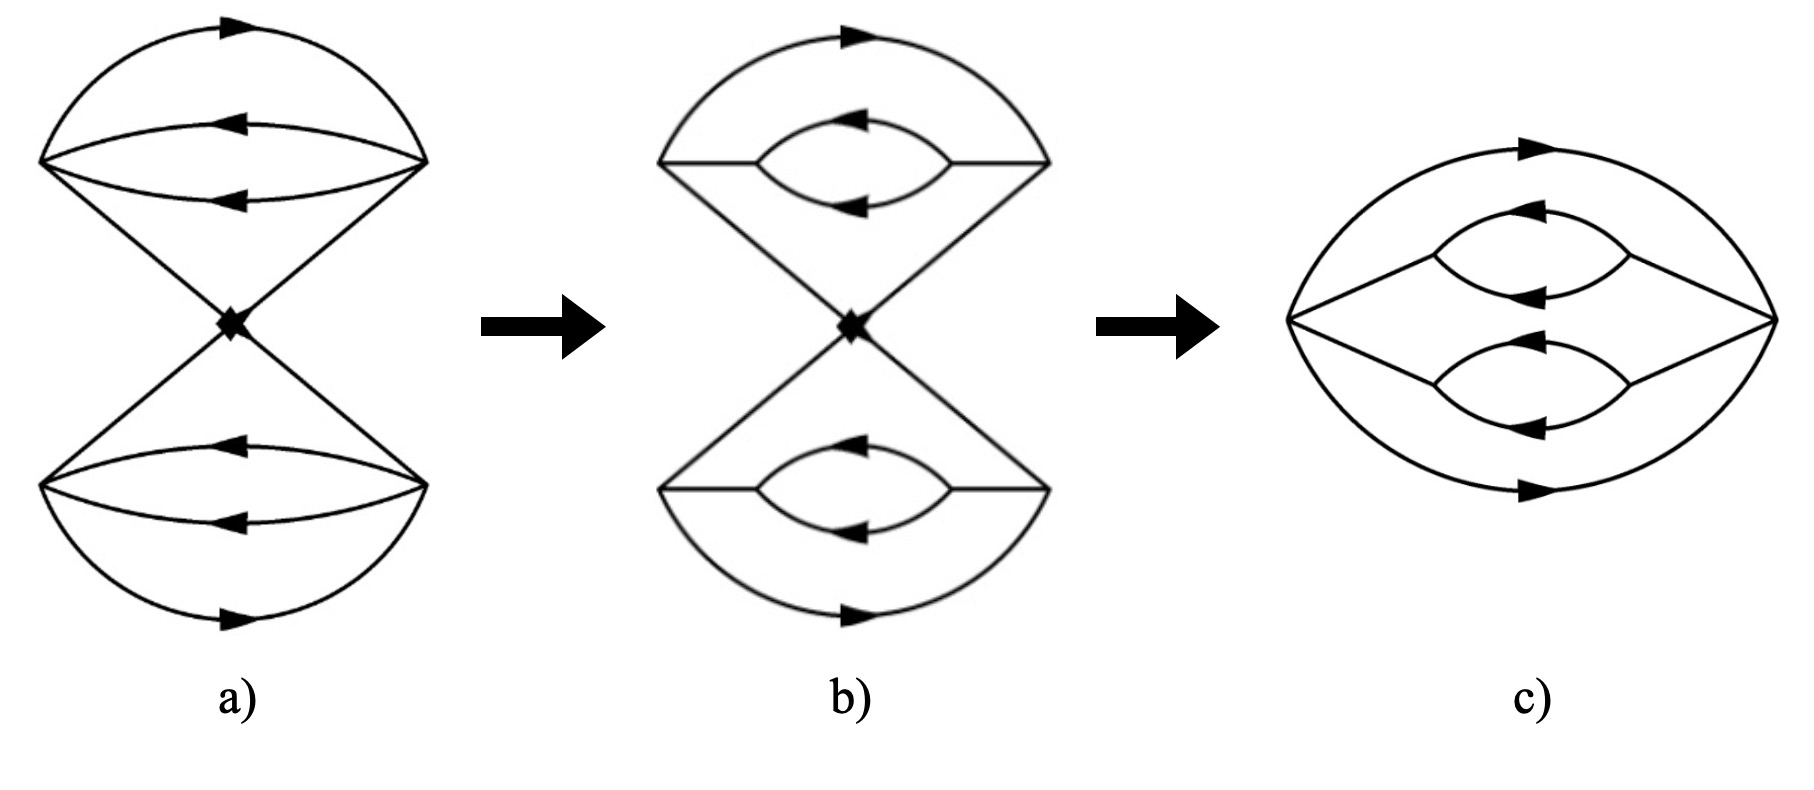
\includegraphics[scale=0.2]{pccd_evo.jpg}
    \caption{Pair-Goldstone contraction schematic}
    \label{fig:pgd_cont}
\end{figure}

Note that we actually reduced the number of summed indices by three despite only having eight contractions (which would normally result in a reduction of 2 indices). This occurs because we are working with a pair operators. To see this, note that the products $\delta_{i+j+}\delta_{i-k-}$ and $\delta_{p-j-}\delta_{p+k+}$ imply $\delta_{pi}\delta_{ji}\delta_{ki}$. That is, the indices $p$, $j$, and $k$, all go to $i$. This "additional" contraction is not immediately obvious from the traditional Goldstone diagram (Figure \ref{fig:pgd_cont}a). However, it is in the pair-Goldstone diagram representation (Figures \ref{fig:pgd_cont}b and \ref{fig:pgd_cont}c). Here, each vertex is replaced with a solid line, one end of which is exclusively for particle lines while the other is exclusively for hole lines. There will always be two lines going into each end; one for the $+$ state of the pair and the other for the $-$ state. This allows one to visually capture the phenomenon of pairs of fermionic operators contracting to operators with differing indices. Notice that in Figure \ref{fig:pgd_cont}b, the hole lines of the top $T_p$ operator are $i+$ and $j-$, while the hole lines of the bottom $T_p$ operator are $i-$ and $j+$. This clearly implies that the bottom indices of both $t$ terms should be $i$. This is visually shown in the "contracted diagram " Figure \ref{fig:pgd_cont}c, in which the hole ends of the $T_p$ lines have been brought or "contracted" together. This additionally resulting in the merging of the $i+$ and $j-$ lines, as well as the $i-$ and $j+$ lines. The lines are now labeled (from top to bottom) $i+$, $a+$, $a-$, $b-$, $b+$, $i-$. Note that because of all this, the final expression (\ref{pgd_final}) can be immediately read from the pair-Goldstone representation (Figure \ref{fig:pgd_cont}c).

We now use pair-Goldstone diagrams to calculate the term $\bra*{\Phi^a_i}V_pT^2_p\ket{\Phi}$ (\ref{long_cont}). That is, the pair-Goldstone diagrams from Figure \ref{fig:pgd} result in the following expressions
\begin{align}
\label{pgda}
a) &\to  2\sum_{bj}g^j_bt^b_jt^a_i
\\
b) &\to  2\sum_{bj}g^j_bt^a_jt^b_i
\\
c) &\to -4\sum_{b}g^i_bt^b_it^a_i
\\
d) &\to -4\sum_{j}g^j_at^a_jt^a_i
\\
\label{pgde}
e) &\to  4g^i_at^a_it^a_i
.\end{align}
The minus signs in front of the expressions resulting from diagrams c) and d) come from the fact that their pre-contracted diagrams (see for example Figure \ref{fig:pgd_cont}b) contain an odd number of crossings. This can be immediately obtained from the contracted diagrams by counting the number of pairs of ends of solid lines that have been merged; in diagrams c) and d), one pair of ends has been merged (either the hole ends or the particle ends) resulting in a prefactor sign of $(-1)^1$, while in diagram e), two pairs of ends have been merged (both the hole ends and the particle ends) resulting in a prefactor sign of $(-1)^2$. The pre-factors of the expressions resulting from diagrams a) and b) can be determined by counting the number of symmetries in each diagram (the same as in standard Goldstone diagrams) for which each is 2. The pre-factors of the contracted diagrams c), d), and e) can be determined by counting the number of unique ways that each of these diagrams can be created by contracting the un-contracted diagrams, a) and b), for which each is four(two from each un-contracted diagram).

\begin{figure}[t]
    \centering
    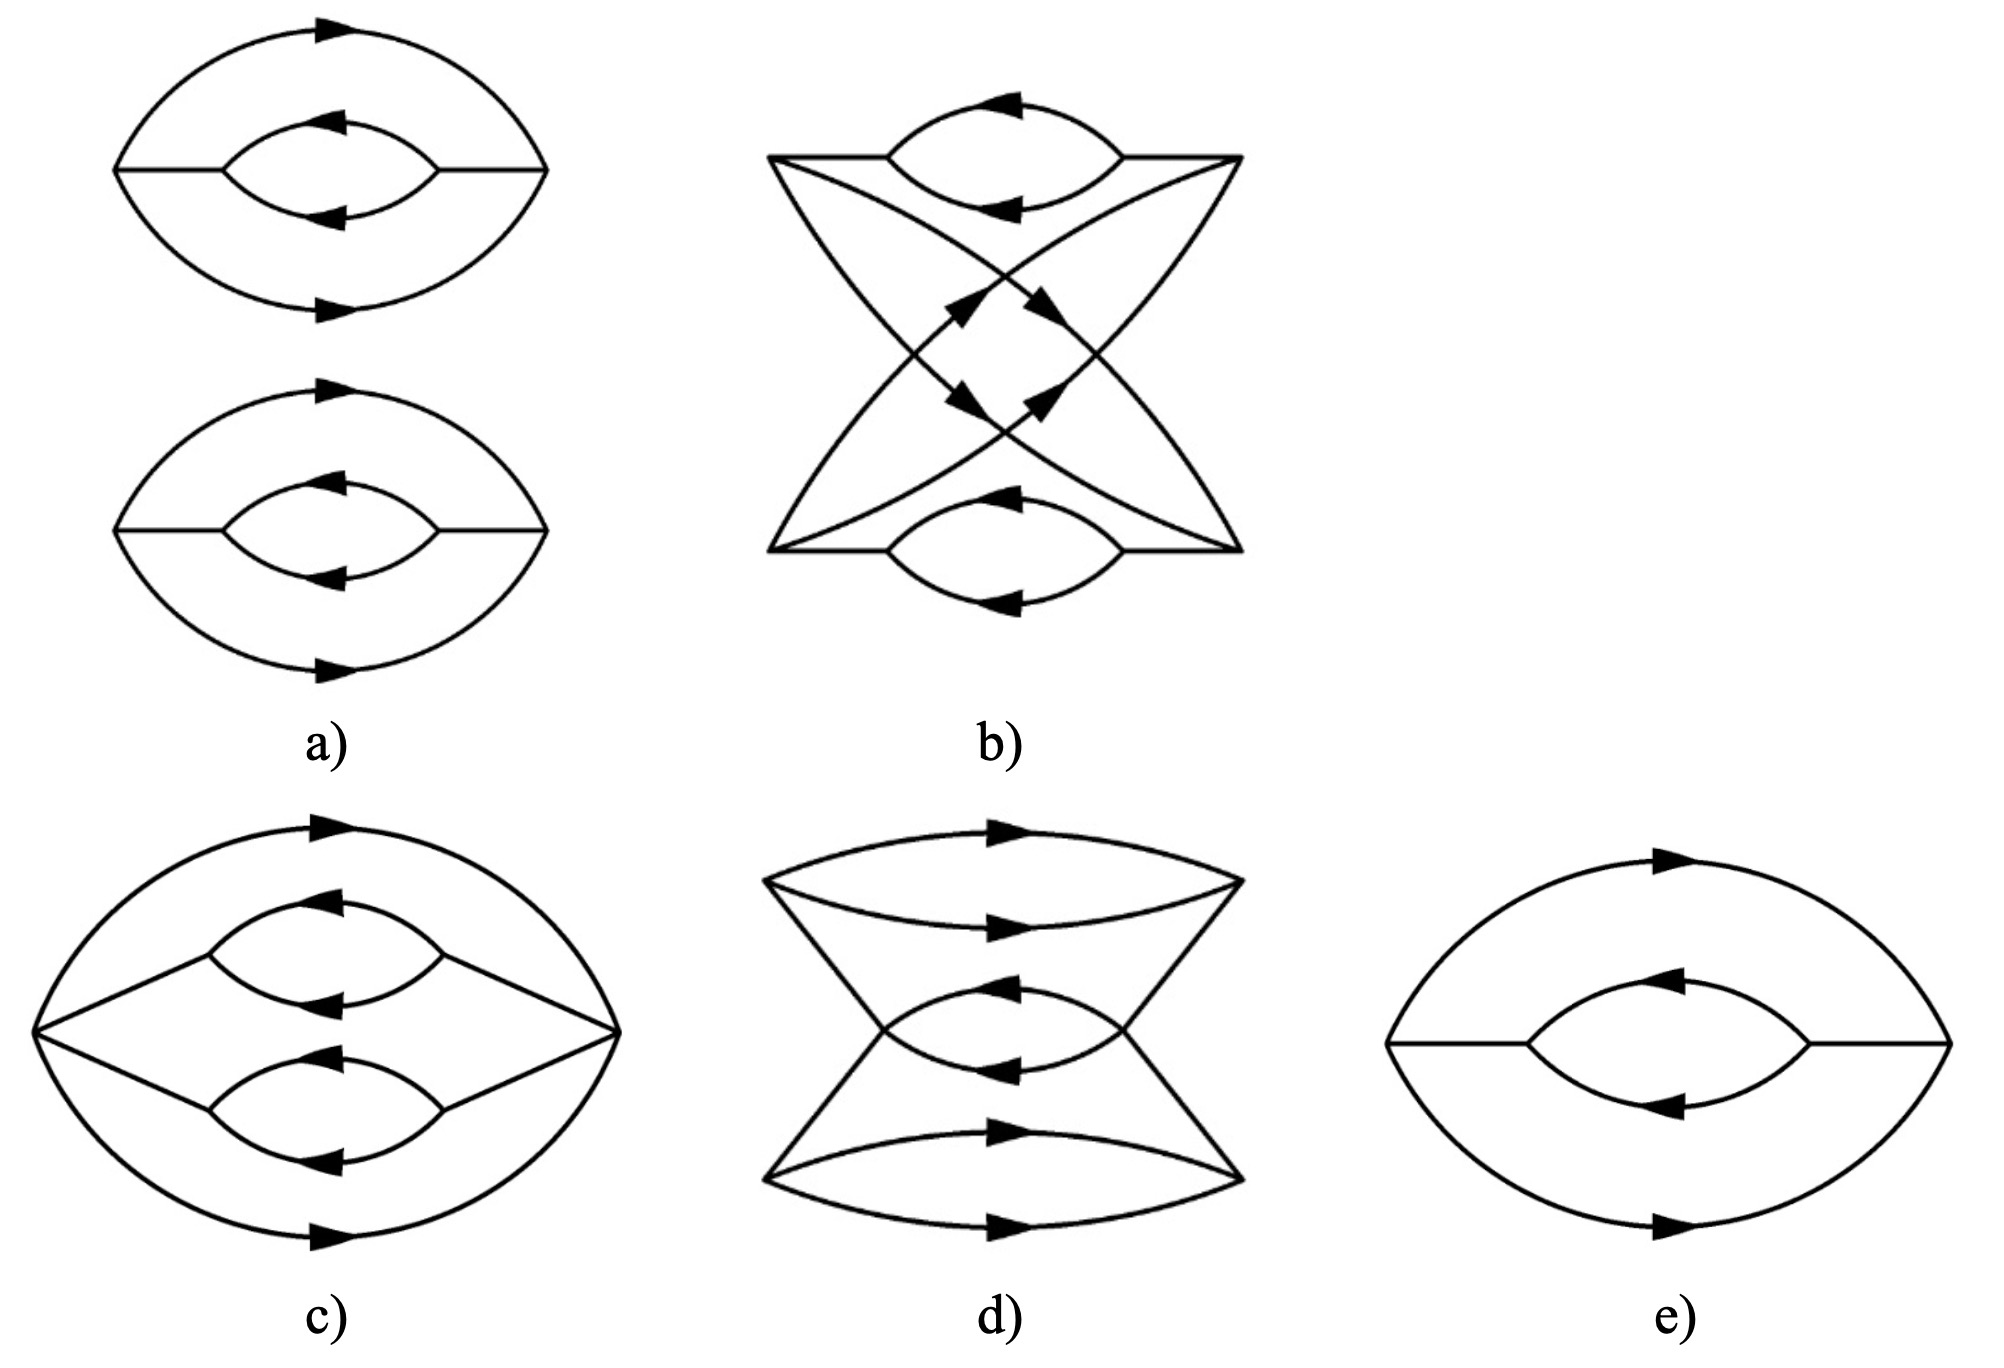
\includegraphics[scale=0.2]{pccd_diagrams.jpg}
    \caption{Pair-Goldstone diagrams for the pairing model.}
    \label{fig:pgd}
\end{figure}

Plugging these resulting expression (\ref{pgda})-(\ref{pgde}) into \ref{long_cont} gives us
\begin{align}
\frac{1}{2}\bra*{\Phi_i^a}V_pT_p^2\ket{\Phi}
=
\sum_{bj}g^j_bt^b_jt^a_i
+\sum_{bj}g^j_bt^a_jt^b_i
-2\sum_{b}g^i_bt^b_it^a_i
-2\sum_{j}g^j_at^a_jt^a_i
+2g^i_at^a_it^a_i
.\end{align}
All together, the pCCD correlation energy equation (\ref{pccd_e_corr}) becomes
\begin{align}
\label{pccd_e_exp}
\Delta E=\sum_{ia}g_a^it_i^a
,\end{align}
while the pCCD amplitude equations (\ref{trunc_pccd_eq}) become
\begin{align}
\label{pccd_eq_exp}
0=g^a_i+2\Big{(}d_a-d_i-g^i_i+g^i_at^a_i-\sum_bg^i_bt^b_i-\sum_jg^j_at^a_j\Big{)}t^a_i+\sum_bg^a_bt^b_i+\sum_jg^j_it^a_j+\sum_{bj}g^j_bt^a_jt^b_i
.\end{align}
In practice, the amplitudes $t$ are solved for by solving the amplitude equation (\ref{pccd_eq_exp}), which is non-linear and coupled, via an iterative root finding algorithm such as Newton's method and plugging them into the energy equation (\ref{pccd_e_exp}).

Although we were able to skip over deriving the reference energy of the pairing model in the previous section because we only cared about the correlation energy $\Delta E$, we will need an expression for the reference energy when we turn to implementing unitary pair coupled cluster (UpCC) theory as the ansatz for the variational quantum eigensolver (VQE). Thus, we derive said expression here using Wick's theorem as follows
\begin{align}
E_{\text{ref}}
&=
\mel{\Phi}{H_p}{\Phi}
\nonumber
\\
&=
\mel*{\Phi}{F_p}{\Phi}
+
\mel{\Phi}{V_p}{\Phi}
\nonumber
\\
&=
\sum_{p\sigma}d_p\mel{\Phi}{
\contraction{}{a}{^\dagger_{p\sigma}}{a}
{a^\dagger_{p\sigma}a_{p\sigma}}
}{\Phi}
+
\sum_{pq}g_q^p\mel{\Phi}{
\contraction[1ex]{a^\dagger_{p+}}{a}{^\dagger_{p-}}{a}
\contraction[2ex]{}{a}{^\dagger_{p+}a^\dagger_{p-}a_{q-}}{a}
a^\dagger_{p+}a^\dagger_{p-}a_{q-}a_{q+}
}{\Phi}
\nonumber
\\
&=
2\sum_pd_ph(p)+\sum_{pq}g_q^ph(p)\delta_{pq}
\nonumber
\\
&=
\sum_i(2d_i+g_i^i)
.\end{align}
In order to find the amplitudes $t$, Newton's method must converge, which required a good initial guess for each $t$. To find one, we turn to many-body perturbation theory.

To assess the performance of our upcoming quantum solution to the pairing model, we benchmark it against pair coupled cluster doubles (pCCD) which can be seen as its classical analog as it employs the exact same ansatz. The pair coupled cluster doubles equations (\ref{cc_energy} and \ref{cc_eq}) become
\begin{align}
\label{pccd_energy} 
E&=\mel{\Phi_0}{\overline{H}_p}{\Phi_0}
\\
\label{pccd_eq}
0&=\mel*{\Phi_i^a}{\overline{H}_p}{\Phi_0}
,\end{align}
where the similarity transformed pairing Hamiltonian is
\begin{align}
\overline{H}_p=e^{-T_p}H_pe^{T_p}
,\end{align}
which can be expanded via the BCH identity as
\begin{align}
\label{sim_H_p}
\overline{H}_p=H_p+\comm{H_p}{T_p}+\frac{1}{2}\comm{\comm{H_p}{T_p}}{T_p}+\cdots
.\end{align}
When the expanded form of the similarity transformed pairing Hamiltonian (\ref{sim_H_p}) is inserted into the pCCD equations (\ref{pccd_energy} and \ref{pccd_eq}), one can truncate the resulting expressions by noting that only certain terms in the infinite sum (those which can be fully contracted) are non-zero. The truncated pCCD equations are
\begin{align}
\label{trunc_pccd_e}
E
&=
\bra*{\Phi}F_p+V_p+V_pT_p\ket{\Phi}
\\
\label{trunc_pccd_eq}
0
&=
\bra*{\Phi_i^a}V_p+F_pT_p+V_pT_p+\frac{1}{2}V_pT_p^2-T_pV_pT_p\ket{\Phi}
,\end{align}
where
\begin{align}
F_p
&=
\sum_pd_pN_p
\\
V_p
&=
\sum_{pq}g^p_qA^\dagger_pA_q
,\end{align}
as we've conveniently separated the pairing model Hamiltonian a single-body and two-body term: $H_p=F_p+V_p$. Recognizing that the first two terms of the truncated pCCD energy equation (\ref{trunc_pccd_eq}) equal the reference energy, the pCCD correlation energy equation is
\begin{align}
\label{pccd_e_corr}
\Delta E = \mel{\Phi}{V_pT_p}{\Phi}
.\end{align}
Using Wick's theorem, the pCCD correlation energy equation (\ref{pccd_e_corr}) becomes
\begin{align}
\label{pccd_e_exp}
\Delta E=\sum_{ia}g_a^it_i^a
,\end{align}
while the pCCD amplitude equations (\ref{trunc_pccd_eq}) become
\begin{align}
\label{pccd_eq_exp}
0
&=
g^a_i+2\Big{(}d_a-d_i-g^i_i+g^i_at^a_i-\sum_bg^i_bt^b_i-\sum_jg^j_at^a_j\Big{)}t^a_i
\nonumber
\\
&+
\sum_bg^a_bt^b_i+\sum_jg^j_it^a_j+\sum_{bj}g^j_bt^a_jt^b_i
.\end{align}
In practice, the amplitudes $t$ are solved for by solving amplitude equation (\ref{pccd_eq_exp}), which is non-linear and coupled, via an iterative root finding algorithm such as Newton's method and plugging them into the energy equation (\ref{pccd_e_exp}).

In order to find the amplitudes $t$, Newton's method must converge, which required a good initial guess for each $t$. To find one, we turn to many-body perturbation theory.

\section{Quantum Solutions}

\subsection{Mapping the Hamiltonian}

To solve the pairing model on a quantum computer, we must create a mapping between the energy levels and qubits. To do so, we simply let qubit $p$ represent energy level $p$. In our pairing scheme, the qubit being either in state $\ket{0}$ or $\ket{1}$ implies that its corresponding energy level is either completely unoccupied or occupied by a pair of fermions, respectively. Note that there is no possibility for broken pairs in this mapping. Now that we've chosen a state to qubit mapping, we must transform the Hamiltonian accordingly, from fermionic operators to spin operators. To do so, we'll first separate the pairing Hamiltonian (\ref{pairing_model_hamiltonian})
into strict one-body and two-body terms, as follows
\begin{align}
\label{pairing_model_hamiltonian_strict}
H
=
\frac{1}{2}\sum_{p=1}^P(2d_p+g^p_p)N_p
+\sum_{\substack{p,q=1 \\ p\neq q}}^Pg^p_qA^\dagger_pA_q
,\end{align}
which follows from the fact that, when $p=q$ in the second sum of ($\ref{pairing_model_hamiltonian}$), it results in the operator
\begin{align}
A^\dagger_pA_p
&=
\left(\frac{X_p-iY_p}{2}\right)\left(\frac{X_p+iY_p}{2}\right)
\\
&=
\frac{I_p-Z_p}{2}
\\
\label{np/2}
&=
\frac{N_p}{2}.
\end{align}
Using the pair-fermionic anti-commutation relation (\ref{AAd_comm}) and applying the Jordan-Wigner transformation to (\ref{np/2}) yields
\begin{align}
\frac{N_p}{2}
&=
\frac{1}{2}
\left(I_p-\delta_{pq}\comm*{A_p}{A^\dagger_q}\right)
\\
&=
\frac{1}{2}
\left(I_p-\frac{1}{4}\delta_{pq}\comm*{X_p+iY_p}{X_q-iY_q}\right)
\\
&=
\frac{I_p-Z_p}{2}.
\end{align}
To deal with the second term of (\ref{pairing_model_hamiltonian_strict}), we note that the sum can be broken up as
\begin{align}
\sum_{\substack{p,q=1 \\ p\neq q}}^Pg^p_qA^\dagger_pA_q
&=
\sum_{\substack{p,q=1 \\ p<q}}^Pg^p_qA^\dagger_pA_q
+
\sum_{\substack{p,q=1 \\ q<p}}^Pg^p_qA^\dagger_pA_q
\\
\label{aa_sum2}
&=
\sum_{\substack{p,q=1 \\ p<q}}^Pg^p_qA^\dagger_pA_q
+
\sum_{\substack{p,q=1 \\ p<q}}^Pg^p_qA^\dagger_qA_p
\\
\label{aa_sum3}
&=
\sum_{\substack{p,q=1 \\ p<q}}^Pg^p_q(A^\dagger_pA_q+A_pA^\dagger_q)
,\end{align}
where we've swapped the indices $p\leftrightarrow q$ to obtain (\ref{aa_sum2}) and used the fact that $\comm*{A_p}{A^\dagger_q}=0$ for $p\neq q$ (which $p<q$ implies) to obtain (\ref{aa_sum3}). Applying the Jordan-Wigner transformation to (\ref{aa_sum3}) yields
\begin{align}
A^\dagger_pA_q+A_pA^\dagger_q
&=
\left(\frac{X_p-iY_p}{2}\right)\left(\frac{X_q+iY_q}{2}\right)
+
\left(\frac{X_p+iY_p}{2}\right)\left(\frac{X_q-iY_q}{2}\right)
\\
&=
\frac{X_pX_q+Y_pY_q}{2}.
\end{align}
All together, the pairing Hamiltonian (\ref{pairing_model_hamiltonian_strict}), after Jordan-Wigner transformation, becomes
\begin{align}
\label{pairing_model_hamiltonian_mapped}
H
=
\frac{1}{2}\sum_{p=1}^P(2d_p+g^p_p)(I_p-Z_p)
+
\frac{1}{2}\sum_{\substack{p,q=1 \\ p<q}}g^p_q(X_pX_q+Y_pY_q).
\end{align}

\subsection{Mapping the Ansatz}

As an ansatz for the pairing model, we choose the unitary pair coupled cluster doubles (UpCCD) ansatz, which is the unitary version of the pair coupled cluster doubles (pCCD) ansatz. It is chosen because any quantum ansatz must be unitary, as all quantum gates must be unitary, it is a pairing ansatz, and includes only up to doubles which allows for the use of, at most, efficiently decomposable two-qubit gates. It is given by
\begin{align}
\ket{\Psi}=e^{T_p-T^\dagger_p}\ket{\Phi}.
\end{align}
Recalling that $T_p$, as defined in (\ref{T_p}), is given by
\begin{align}
T_p=\sum_{ia}t^a_iA^\dagger_aA_i,
\end{align}
turns the ansatz into the variational form
\begin{align}
\label{pair_fermionic_ansatz}
\ket{\Psi(t)}
&=\exp\left\{\sum_{ia}t^a_i\left(A^\dagger_aA_i-A^\dagger_iA_a\right)\right\}\ket{\Phi_0}
\\
&=\exp\left\{\sum_{ia}t^a_i\left(A^\dagger_aA_i-A_aA^\dagger_i\right)\right\}\ket{\Phi_0},
\end{align}
where we've used the fact that $\comm*{A_a}{A^\dagger_i}=0$ for since, by definition $a\neq i$. Applying the Jordan Wigner transformation to the operators yields
\begin{align}
A_a^{\dagger}A_i-A_aA_i^{\dagger}
&=
\left(\frac{X_a-iY_a}{2}\right)\left(\frac{X_i+iY_i}{2}\right)
-
\left(\frac{X_a+iY_a}{2}\right)\left(\frac{X_i-iY_i}{2}\right)
\\
&=
\frac{i}{2}(X_aY_i-Y_aX_i).
\end{align}
Plugging this back into the ansatz (\ref{pair_fermionic_ansatz}) yields
\begin{align}
\label{pairing_pauli_ansatz}
\ket{\Psi(t)}
=
\exp\left\{\frac{i}{2}\sum_{ia}t^a_i(X_aY_i-Y_aX_i)\right\}\ket{\Phi_0}.
\end{align}
As it is only known how to efficiently decompose two-qubit operators, we must write our ansatz as a sum of two-qubit operators. To achieve this, we employ a simple Suzuki-Trotter approximation \cite{ref:trotter}, which we truncate to a single first-order step in order to minimize the depth of the quantum circuit that will implement it. Doing so yields
\begin{align}
\label{pairing_trott_ansatz}
\ket{{\Psi}(t)}
=
\prod_{ia}A^a_i\ket{\Phi_0},
\end{align}
where we've defined the two-qubit operator
\begin{align}
\label{aia}
A_i^a=\exp\left\{\frac{i}{2}t^a_i(X_aY_i-Y_aX_i)\right\}
,\end{align}
which is efficiently decomposable. One could consider higher order Trotterizations or multiple Trotter steps; however, employing these would substantially increase the depth of the circuit. Additionally, it will be seen later that our simple Trotter approximation provides a sufficient ansatz for VQE to be able to minimize the energy. The operator $A^a_i$ takes the following matrix form
\begin{align}
A^a_i
=
\begin{pmatrix}
1 & 0 & 0 & 0 \\
0 & \cos(t^i_a) & \sin(t^i_a) & 0 \\
0 & -\sin(t^i_a) & \cos(t^i_a) & 0 \\
0 & 0 & 0 & 1
\end{pmatrix}
.\end{align}
From this matrix form, one can see that $A^a_i$ acts non-trivially only in the two-qubit subspace $\{\ket{01},\ket{10}\}$ and is closed in said subspace. This means that as long as we initialize our quantum circuit to a bit-string state with Hamming weight equal to the number of particles, we're guaranteed (save for noise) to only search the relevant subspace of the Hamiltonian.

\subsection{Implementing the Ansatz}

Now that we've mapped the ansatz to spin operators, we must now determine how to efficiently decompose it into a quantum circuit given the limitations of qubit connectivity and circuit depth allowed on NISQ devices. Here, we give two such methods; the first is for a quantum computer with linear connectivity while the second is for one with circular connectivity. 

To define these two connectivity terms, consider a quantum computer with $N$ qubits. Label and order the qubits as $0,2,...,N-1$.
A quantum computer has linear connectivity when each of its qubits, except for the first and last, is connected to its left and right neighboring qubits.
This is visualized in Figure \ref{fig:linear_con} where the qubits are connected if the circles representing them are connected in the graph.
\begin{figure}
\centering
\begin{tikzpicture}
\begin{center}
\draw [thick, gray] (0,0) -- (4.5,0);
\node[circle,draw=black,fill=white!80!black,minimum size=1cm] at (0,0) {$q_1$};
\node[circle,draw=black,fill=white!80!black,minimum size=1cm] at (1.5,0) {$q_2$};
\node[circle,draw=black,fill=white!80!black,minimum size=1cm] at (3,0) {$\cdots$};
\node[circle,draw=black,fill=white!80!black,minimum size=1cm] at (4.5,0) {$q_{N}$};
\end{center}
\end{tikzpicture} 
\caption{Linear connectivity of qubits schematic.}
\label{fig:linear_con}
\end{figure}
A quantum computer has circular connectivity when each of its qubits (including the first and last) is connected to its left and right neighboring qubits. This is visualized in Figure \ref{fig:circular_con}.
\begin{figure}
\centering
\begin{tikzpicture}
\begin{center}
\node[circle,draw=black,minimum size=2cm] at (3,0) {};
\node[circle,draw=black,fill=white!80!black,minimum size=1cm] at (3,1) {$q_1$};
\node[circle,draw=black,fill=white!80!black,minimum size=1cm] at (4,0) {$q_2$};
\node[circle,draw=black,fill=white!80!black,minimum size=1cm] at (3,-1) {$\cdots$};
\node[circle,draw=black,fill=white!80!black,minimum size=1cm] at (2,0) {$q_{N}$};
\end{center}
\end{tikzpicture}   
\caption{Circular connectivity of qubits schematic.}
\label{fig:circular_con}
\end{figure}
The ansatz is implemented using what we'll call the particle-hole swap network (phsn) technique which has both a linear \cite{ref:phsn} and circular connectivity (novel) version. An illustration of the circuits for the four-particle, five-hole system for both connectivities are given in Figure \ref{fig:circuits}.

\begin{figure}[h]
\begin{centering}
\begin{subfigure}[t]{0.3\textwidth}
\hspace*{-10mm}
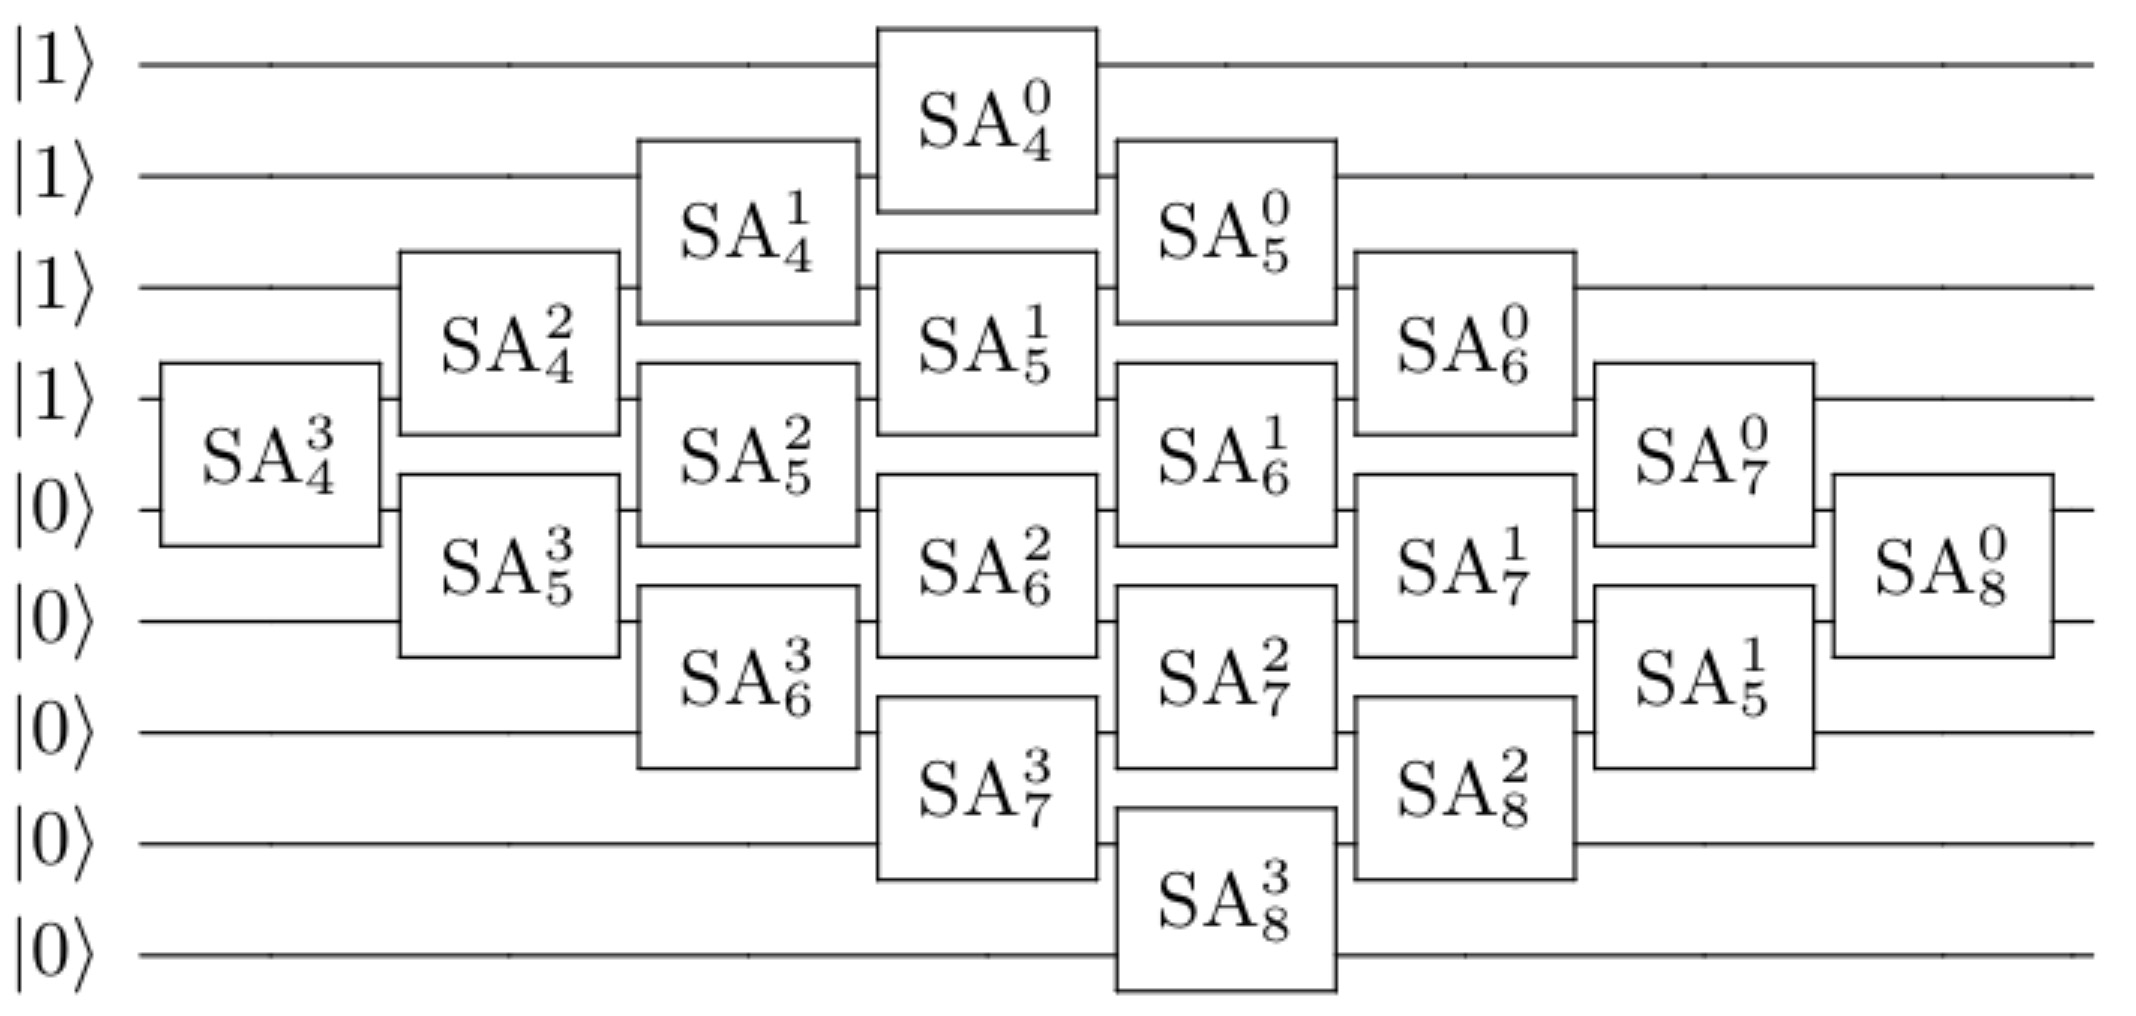
\includegraphics[scale=0.118, left]{linear_ph_circuit.jpg}
\caption{}
\label{linear_circuit}
\end{subfigure}
\hspace{4cm}
\begin{subfigure}[t]{0.3\textwidth}
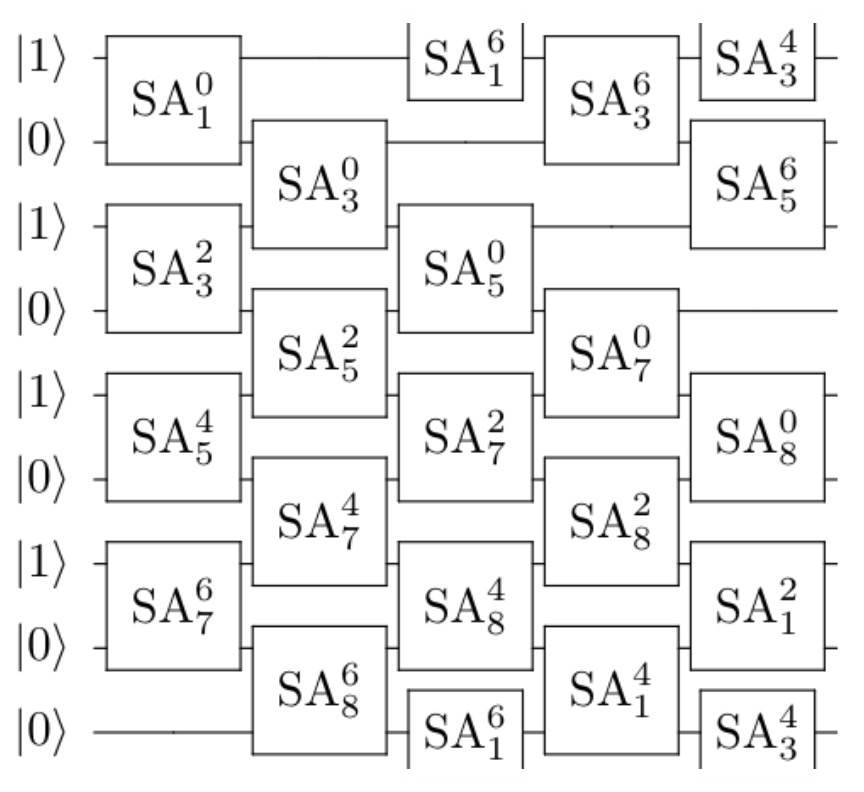
\includegraphics[scale=0.191, left]{circular_ph_circuit.jpg}
\caption{}
\label{circular_circuit}
\end{subfigure}
\caption{a) Linear particle-hole swap network (lphsn) for four-particle, five-hole system. b) Circular particle-hole swap network for four-particle, five-hole system (cphsn). See Figure \ref{fig:dots} for schematic representation.}
\label{fig:circuits}
\end{centering}
\end{figure}

\begin{figure}[h]
\centering
\begin{subfigure}[b]{0.4\textwidth}
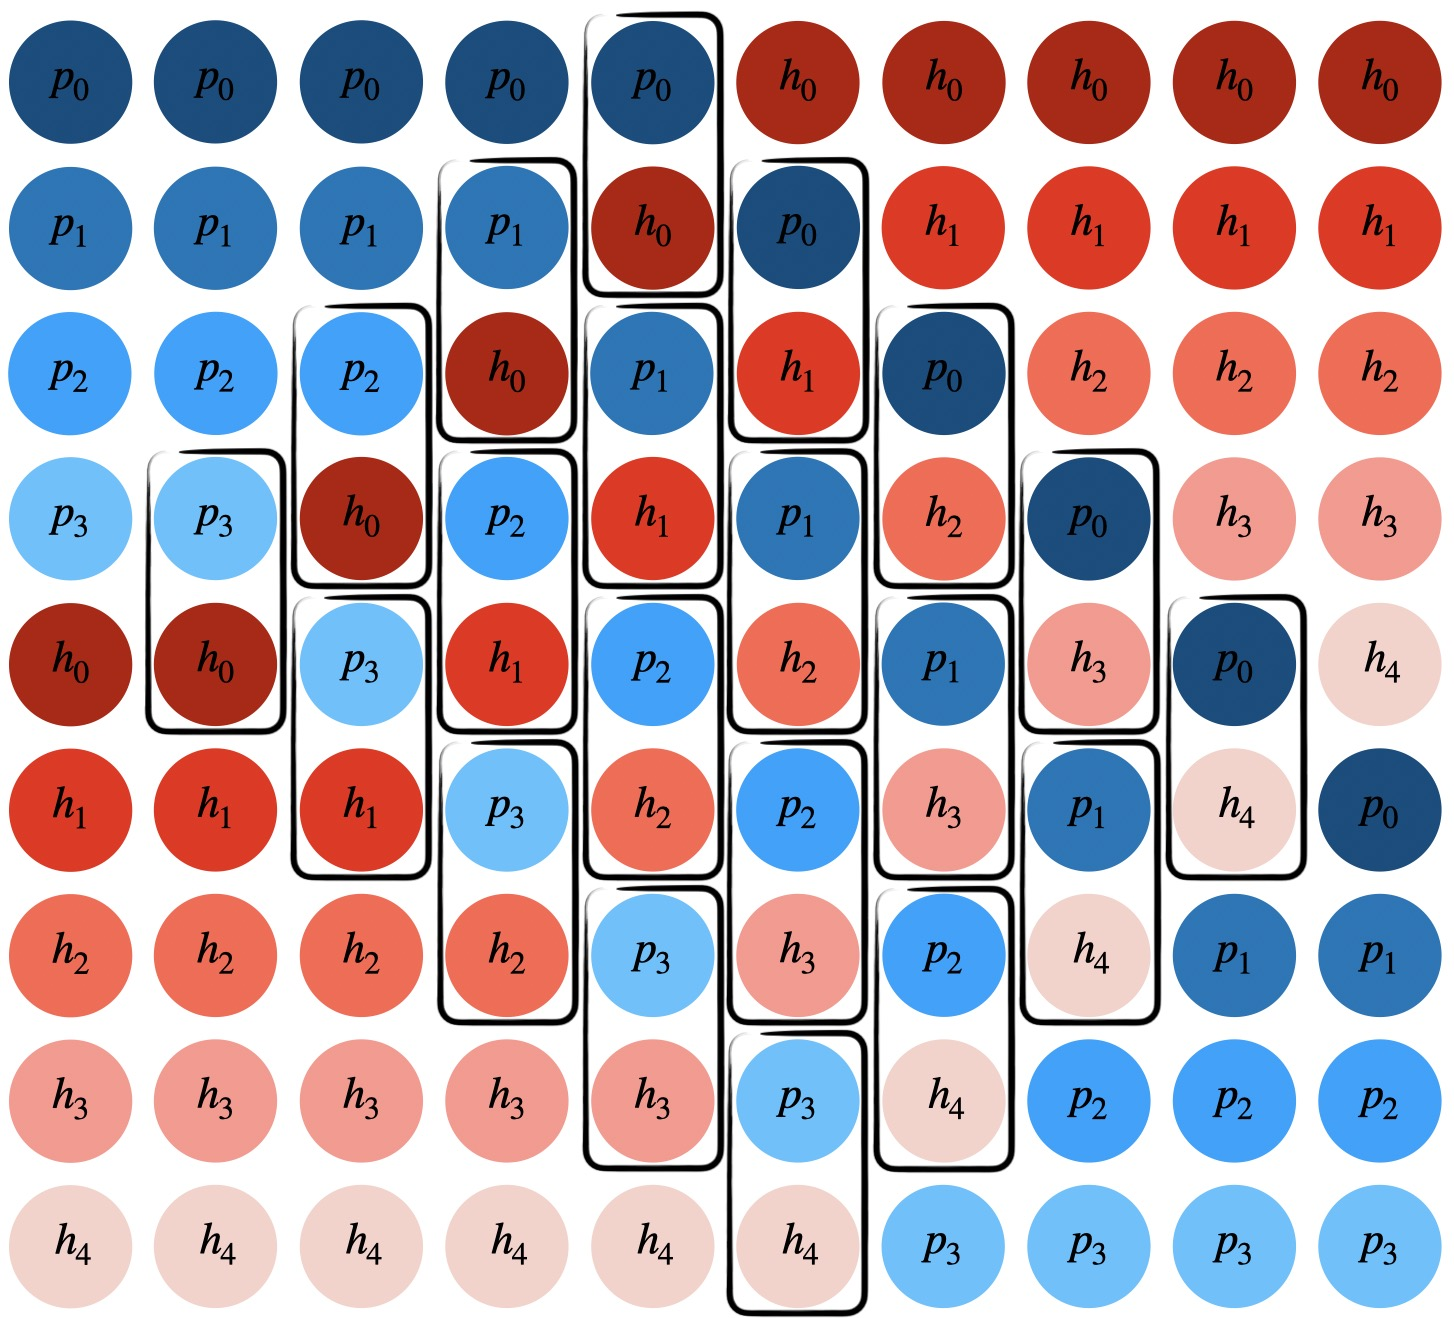
\includegraphics[scale=0.115]{linear_ph_pic.jpg}
\caption{}
\label{fig:linear_dots}
\end{subfigure}
\begin{subfigure}[b]{0.4\textwidth}
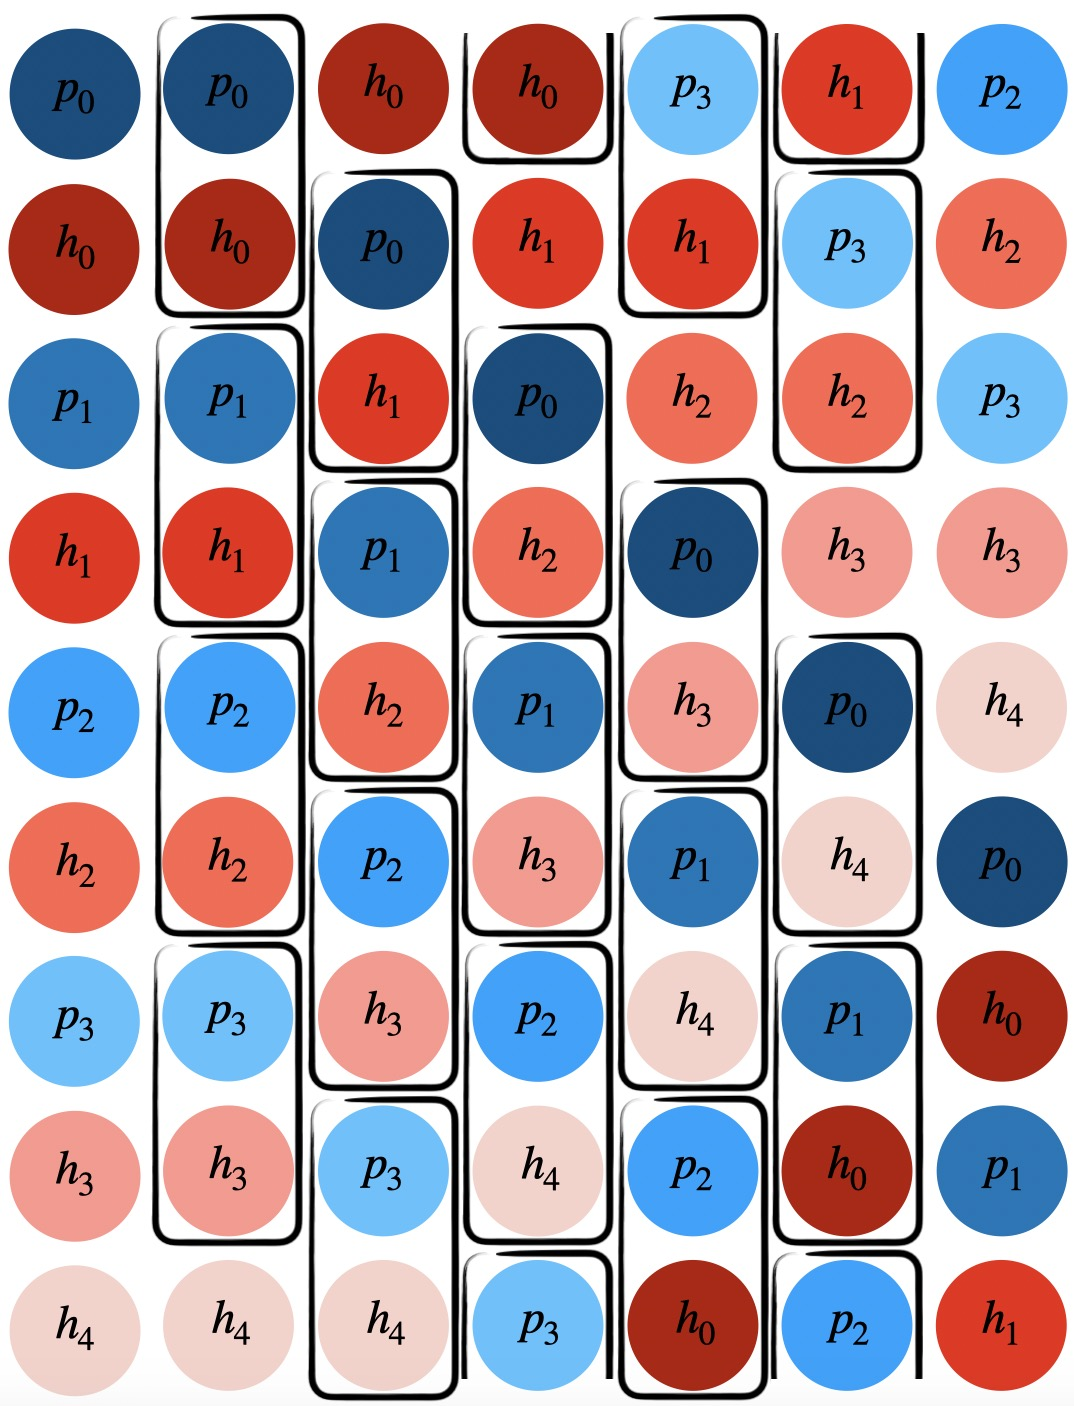
\includegraphics[scale=0.115]{circular_ph_pic.jpg}
\caption{}
\label{fig:circular_dots}
\end{subfigure}
\caption{a) Schematic representation of the linear particle-hole swap network (lphsn). b) Schematic representation of the circular particle-hole swap network (cphsn). Each circle represents a qubit and a slot (particle/hole). The particles are labeled $p_0,...,p_3$ and are colored blue while the holes are labeled $h_0,...,h_4$ and are colored red. The first and last columns of circles are the initial and final positions of the qubits/slots. A rectangle around a pair of circles $p_i,h_j$ denotes that the gate $SA^{p_i}_{h_j}$ has been applied between the corresponding qubits. See Figure \ref{fig:circuits} for circuit representation.}
\label{fig:dots}
\end{figure}

In said circuits, $S$ is the SWAP gate \ref{swap_def} and $A^i_a$ is the two qubit operator defined in (\ref{aia}). Because $SA^i_a \in \text{SO}(4)$, it can be efficiently mapped \cite{ref:kak} to a depth five circuit consisting of two CNOTs and twelve single-qubit gates. The number of two-qubit gates $SA^i_a$ is equal to $G=P(P-N)$. The depth of the linear particle-hole swap network is $D(\text{lphsn})=P-1$ where $P$ is the number of qubits (energy-levels in the pairing model). The depth of the circular particle-hole swap network, however, is $D(\text{cphsn})=\max(N,P-N)$ where $N$ is the number of particles (Hamming weight of the initial state). Because $N$ is bounded as $1\leq N\leq P$, we have that the depth of the cphsn is bounded as $\lceil P/2 \rceil \leq D(\text{cphsn})\leq P-1$. The depth decreases as $N$ approached $P/2$ from either direction, achieving a minimum for $\lceil P/2 \rceil$. Thus, we have that $D(\text{cphsn})\leq D(\text{lphsn})$. That is, the circular connectivity enables a circuit of less than or equal to depth compared to a circuit constrained by linear connectivity, up to reduction by a factor of 2. Shortening the depth of the circuit is vital for decreasing noise on NISQ era devices. The algorithm to implement the linear particle-hole swap network is given below. Here $p$ is the number of energy levels and $n$ is the number of energy levels that are initially filled

\begin{algorithm}[H]

\caption{Linear Particle-Hole Swap Network}\label{lphsn}

\hspace*{\algorithmicindent} \textbf{Input:} Number of energy levels $p$, number of initially  filled energy levels $n$,
\\
\hspace*{\algorithmicindent} gates $\text{SA}^i_a$, and qubit order list
\\
\hspace*{\algorithmicindent} $o=[1,2,...,n]$.
\\
\hspace*{\algorithmicindent} \textbf{Output:} Quantum circuit implementation of lphsn.

\begin{algorithmic}[H]

\State $t = n - 1$ \Comment{index of highest qubit acted upon}
\State $b = n$ \Comment{index of lowest qubit acted upon}
\State $h = 1$ \Comment{height ($\#$ of gates per column)}
\State $d_t = -1$ \Comment{top direction}
\State $d_b = 1$ \Comment{bottom direction}

\For{$0\leq i\leq n-1$}
    \State apply gate $X$ to qubit $i$
\EndFor

\While{$h \neq 0$}
    \For{$0 \leq i \leq h-1$}
        \State $x=t+2i$
        \State apply $\text{SA}^{o[x]}_{o[x+1]}$ to qubits $x$ and $x+1$
        \State $o[x], o[x+1] = o[x+1], o[x]$
    \EndFor
    \If{$t = 1$}
        \State $d_t = 1$
    \EndIf
    \If{$b = p$}
        \State $d_b = -1$
    \EndIf
    \State $t\mathrel{+}=d_t$, $b\mathrel{+}=b_d$, $h = (b-t+1)/2$
\EndWhile
\end{algorithmic}

\end{algorithm}

\begin{algorithm}[H]

\caption{Circular Particle-Hole Swap Network}\label{lphsn}

\hspace*{\algorithmicindent} \textbf{Input:} Number of energy levels $p$, number of initially 
\\
\hspace*{\algorithmicindent} filled energy levels $n$, gates $\text{SA}^i_a$, and qubit order list 
\\
\hspace*{\algorithmicindent} $o=[1,2,...,n]$.
\\
\hspace*{\algorithmicindent} \textbf{Output:} Quantum circuit implementation of cphsn.

\begin{algorithmic}[H]

\State $d = \text{max}(n,p-n)$ \Comment{depth of circuit}
\State $h = \text{min}(n,p-n)$ \Comment{height ($\#$ of gates per column)}

\For{$0\leq i\leq n-1$}
    \State apply gate $X$ to qubit $2i$
\EndFor
\If{$n \geq \lceil p/2 \rceil$}
    \For{$0\leq i\leq p-1$}
    \State apply gate $X$ to qubit $i$
    \EndFor
\EndIf

\For{$0\leq i\leq d-1$}
    \For{$0\leq i\leq h-1$}
        \State $x=(i+2j) \mod{p}$
        \State apply $\text{SA}^{o[x]}_{o[x+1]}$ to qubits $x$ and $x+1$
        \State $o[x], o[x+1] = o[x+1], o[x]$
    \EndFor
\EndFor

\end{algorithmic}

\end{algorithm}

\subsection{Initialization}

As VQE involves a minimization algorithm, it is important that we choose a good initial guess for the variational parameters $t^a_i$ so as to give the classical minimization algorithm the best chance at finding the ground state energy the fastest and with the highest precision. The initial guess we will be using is 
\begin{align}
\label{t_init_copy}
{t^a_i}^{(0)}
=
\frac{1}{2}\frac{g^a_i}{d_i-d_a+g^i_i},
\end{align}
from (\ref{t_init}) which was computed by comparing the pCCD correlation energy with the second order contribution to the correlation energy from MBPT in subsection \ref{subsection:mbpt}. This provides a good initial guess because we know that it results in an energy that is close to the second order contribution to the correlation energy from MBPT, which we know is a good approximation to the true ground state. This mean that our minimizer will start close to the correct solution in the energy landscape through which it must transverse. It also implies that, barring degeneracy, an ansatz initialized to ${t^a_i}^{0}$ should have a significant overlap with the true ground state wavefunction.

Figure \ref{fig:pairing_init_e_comp} compares initial correlation energies ($\mel{\psi(\theta)}{H}{\psi(\theta)}$) between the case where the initial parameters $t^a_i$ are random and where they are informed by many-body perturbation theory, $t_i^a={t_i^a}^{0}$; It uses the pairing model with $P=4$ energy levels and $N=2$ pairs of particles. It can be seen from said figure that the initial correlation energy resulting from $t_i^a={t_i^a}^{0}$ (E$\_$calc$\_$ia) is much closer to the correct ground state correlation energy (E$\_$true) than the initial correlation energy informed resulting from random initial parameters (E$\_$calc$\_$rand). In fact, the randomness of the initial parameters case seems to carry over to the corresponding initial correlation energy as it produces noisy, flat line that is way above the correct correlation energies. Here, we've defined the initial correlation energies as
\begin{align}
\label{initial_energies}
E_{\text{calc\_ia}} &= \mel{\Phi\left({t_i^a}^{0}\right)}{H}{\Phi\left({t_i^a}^{0}\right)},
\\
E_{\text{calc\_rand}} &= \mel{\Phi\left(t_{\text{rand}}^{0}\right)}{H}{\Phi\left(t_{\text{rand}}\right)},
\\
E_{\text{true}} &= \mel{\Phi\left(t_{\text{min}}^{0}\right)}{H}{\Phi\left(t_{\text{min}}\right)},
\end{align}
where $t_{\text{rand}}$ is a set of random parameters while $t_{\text{true}}$ is the set of parameters that minimize the energy.

\begin{figure}[H]
    \centering
    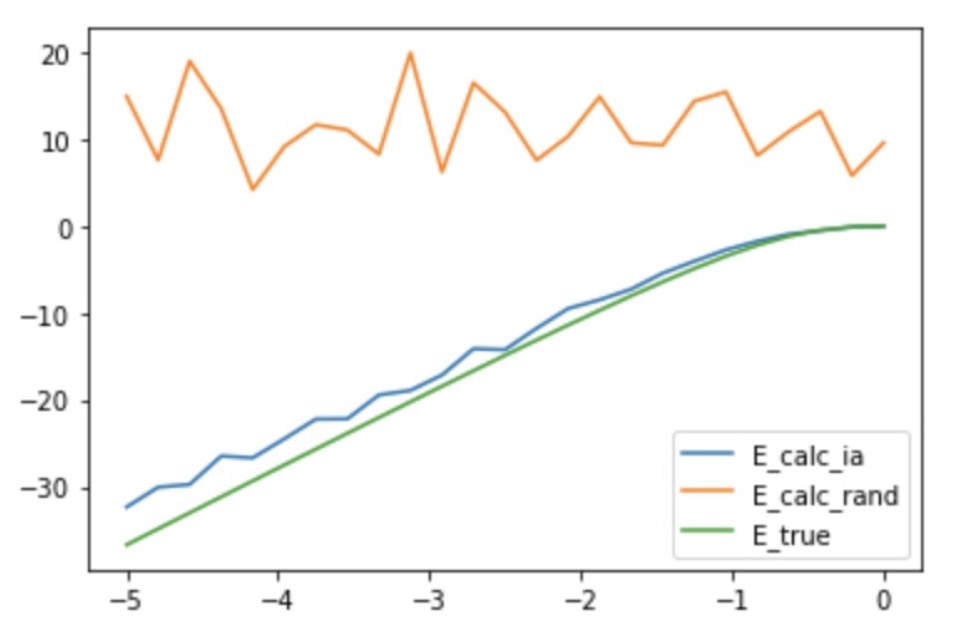
\includegraphics[scale = 0.25]{pairing_init_e_comp.jpg}
    \caption
    {Initial correlation energy using $t_i^a$.}
    \label{fig:pairing_init_e_comp}
    \caption{Initial energies correlation energies for the pairing model with $P=4$ energy levels and $N=2$ pairs of particles are compared. E$\_$calc$\_$ia uses the initial parameters informed by MBPT, E$\_$calc$\_$rand uses random initial parameters, and E$\_$true is the true ground state correlation energy}
\end{figure}

Because (E$\_$calc$\_$ia) is so much closer to (E$\_$true) than (E$\_$calc$\_$rand), the optimization portion of the algorithm should not have to go through as many iterations when using $t_i^a={t_i^a}^{0}$ as opposed to $t_i^a=t_{\text{rand}}$  which is confirmed by Figure \ref{fig:pairing_itr_comp}. This illustrates the importance of initializing one's variational parameters to a good guess rather than just doing so randomly. This requires knowledge about the specific system that one is trying to solve. In this case, we were able to use information from many-body perturbation theory and coupled cluster theory to inform ourselves of a good initial guess.

\begin{figure}[H]
    \centering
    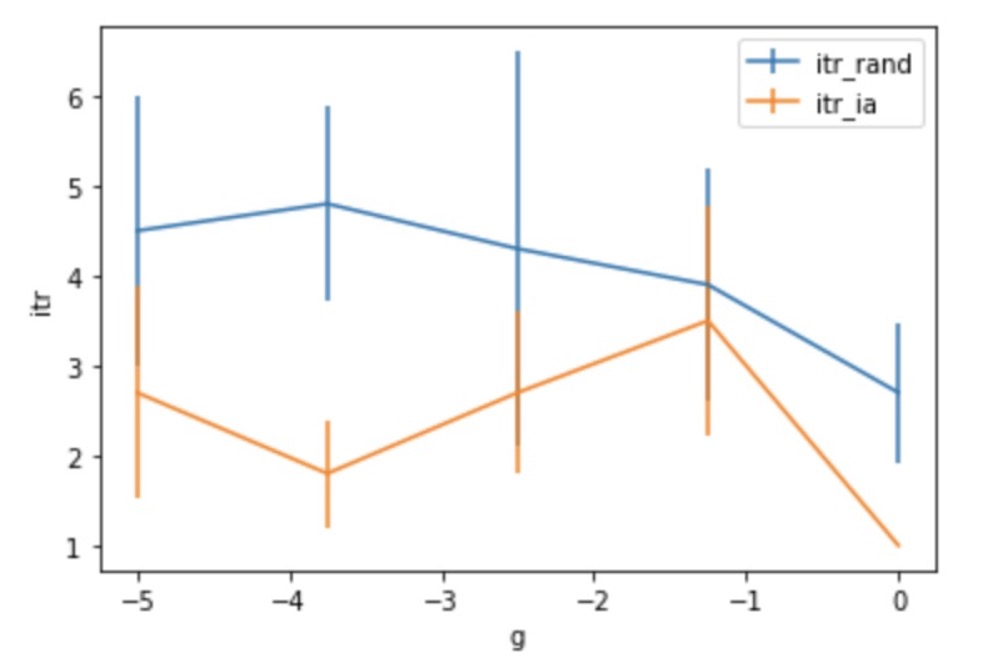
\includegraphics[scale = 0.25]{pairing_itr_comp.jpg}
    \caption{Number of iterations required to minimize the correlation energy (averaged over 10 trials) are compared for the pairing model with $P=4$ energy levels and $N=2$ pairs of particles. itr$\_$rand and itr$\_$ia are the number of iterations required to minimize the correlation energy for random initial parameters and initial parameters informed by MBPT, respectively.}
    \label{fig:pairing_itr_comp}
\end{figure}

Finally, Figure \ref{fig:pairing_itr_e_comp} compares the minimized correlation energy between the two initialization cases, showing that the MBPT informed initial parameterization leads to more accurate predictions of the ground state correlation energy.

\begin{figure}[H]
    \centering
    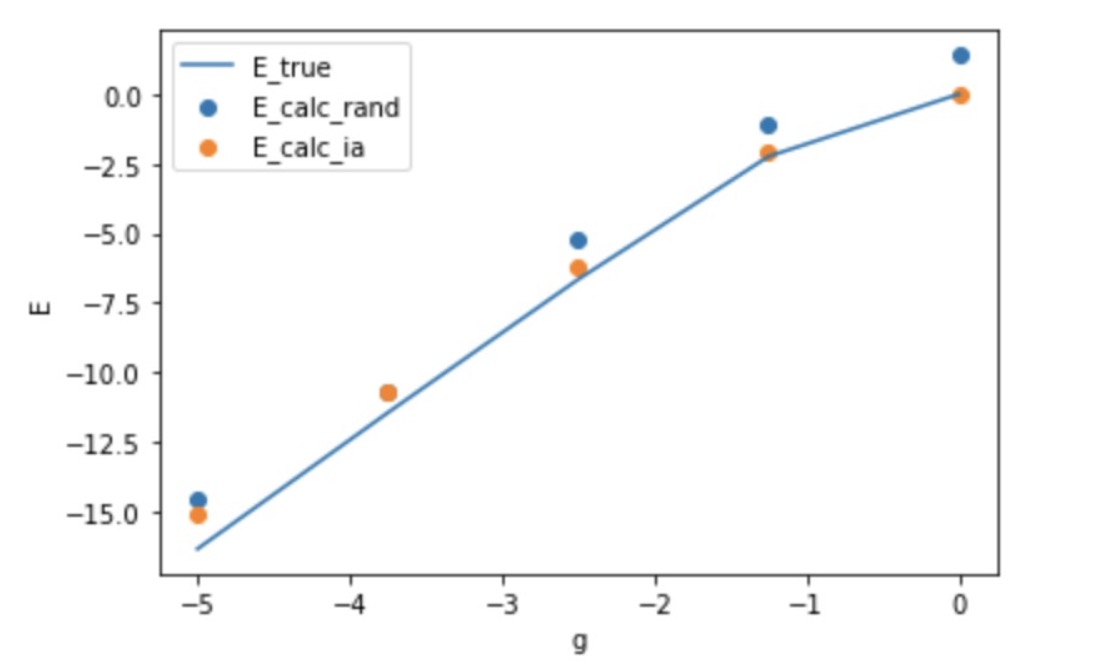
\includegraphics[scale = 0.25]{pairing_itr_e_comp.jpg}
    \caption{VQE calculated ground state correlation energies compared between the case of random initial parameterization (E$\_$calc$\_$rand) and the case of MBPT informed initial parameterization (E$\_$calc$\_$ia)}
    \label{fig:pairing_itr_e_comp}
\end{figure}


\subsection{Results}

To start, we compare the performances of the classical solution (pCCD) with the quantum solution (UpCCD via VQE). In Figure \ref{fig:pairing_plot_vqe_pccd_42} we see such a comparison for the pairing model with $P=4$ energy levels, $N=2$ pairs, linearly increasing singular particle energies $d_p=p$, and constant pairing strength $g_{pq}=g$. The VQE results were computed via a noiseless simulation on a classical computer. We see that for small values of $g$ the two methods perform relatively similarly. However, as the magnitude of $g$ grows, we can clearly see that the quantum solution gives a better estimate of the ground state correlation energy than the classical solution.

\begin{figure}[t]
    \centering
    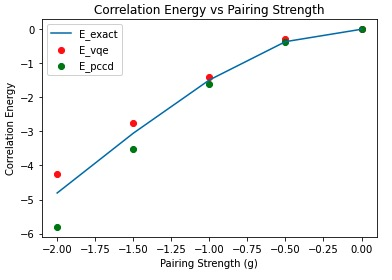
\includegraphics[scale = 0.75]{pairing_plot_vqe_pccd_42.jpg}
    \caption
    {Pairing strength vs ground state correlation energy obtained through exact diagonalization (blue line), the variational quantum eigensolver (red dots) and pair coupled cluster doubles (green dots) for the pairing model with $P=4$ energy levels, $N=2$ pairs, linearly increasing singular particle energies $d_p=p$, and constant pairing strength $g^i_a=g$.}
    \label{fig:pairing_plot_vqe_pccd_42}
\end{figure}

% \begin{figure}[b]
%     \centering
%     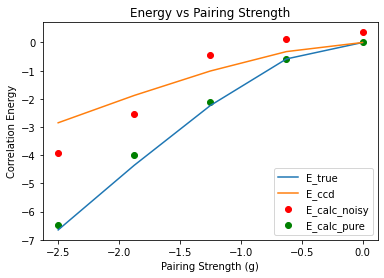
\includegraphics[scale = 0.5]{full_4_2.png}
%     \caption
%     {Exact and Calculated Correlation Energies vs Pairing Strength for $(P,N)=(4,2)$}
%     \label{fig:pairing_init}
% \end{figure}

% \begin{figure}
%     \centering
%     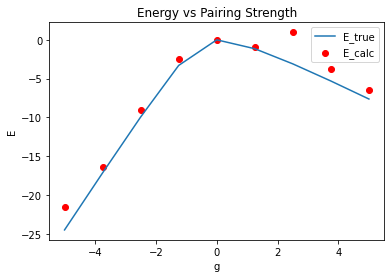
\includegraphics[scale = 0.5]{p=5_n=2_d=lin_g=const.png}
%     \caption{Exact and Calculated Correlation Energies vs Pairing Strength for $(P,N)=(5,2)$}
%     \label{fig:pairing_init}
% \end{figure}

Additionally, we test our VQE ansatz on a non-constant pairing strength pairing model. Here, we choose $g^i_a=gij/(\max{i}\max{j})$ which is clearly a case where $g$ is separable, which is a more realistic approximation to real-world nuclei whose nuclear forces are often modeled to be separable. The function is divided by the maximums of the energy level indices $i$ and $j$ so that the values of $g$ don't vary too wildly. In Figure \ref{fig:g_sep_vqe} we see how pCCD performs well for small absolute values of $g$ but fails for larger values, unlike VQE which gets close to the true correlation energy values for all values of $g$.

\begin{figure}[t]
    \centering
    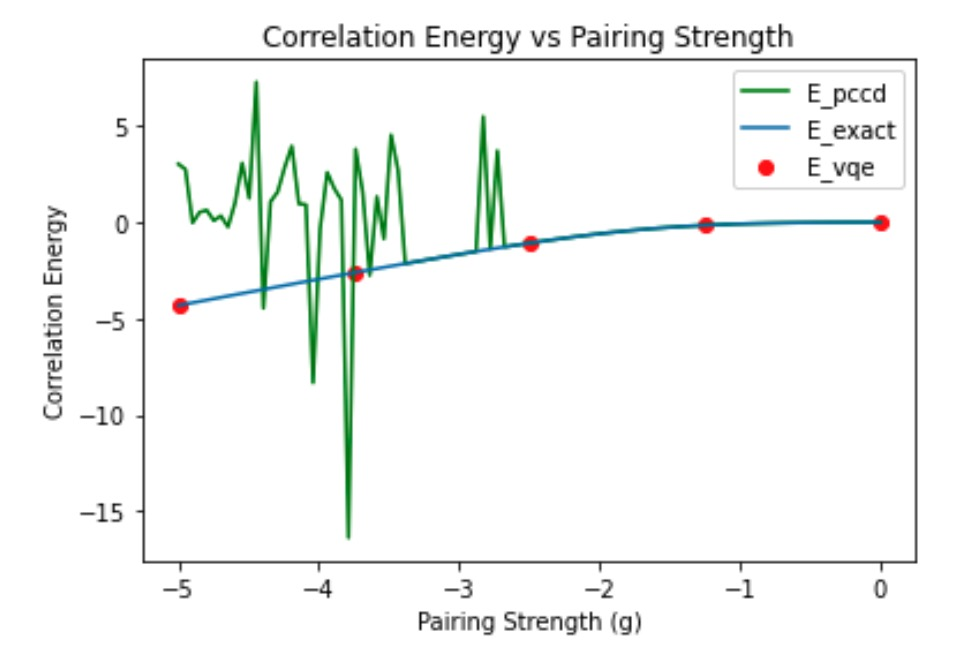
\includegraphics[scale = 0.3]{g_sep_vqe.jpg}
    \caption
    {Pairing strength vs ground state correlation energy obtained through exact diagonalization (blue line), the variational quantum eigensolver (red dots) and pair coupled cluster doubles (green dots) for the pairing model with $P=4$ energy levels, $N=2$ pairs, linearly increasing singular particle energies $d_p=p$, and constant separable pairing strength $g^i_a=gij/(\text{max}(i)(\text{max}(j)$.}
    \label{fig:g_sep_vqe}
\end{figure}

\subsection{Iterative Quantum Excited States Algorithm}

The following is my method to compute the eigenstates of a Hamiltonian and their corresponding energies. Let $\ket{\psi_k}$ represent the $k^{\text{th}}$ eigenstate of the Hamiltonian $H$ with energy $E_n$. That is
$H\ket{\psi_n}=E_n\ket{\psi_n}$.
Assume that $\ket{\psi_k}$ can be parameterized by the set of angles $\theta_k$, that is $\ket{\psi_k}=\ket{\psi(\theta_k)}$. This algorithm is iterative, meaning that to find $E_k$, one must first use the algorithm to compute $E_0$ through $E_k$ and $\theta_0$ through $\theta_k$. Assuming that one has already done this, recall that any state $\ket{\psi(\theta)}$ can be expanded in terms of the $N$ eigenstates of $H$. That is
\begin{align}
\ket{\psi(\theta)}=\sum_{n=0}^{N}\bra{\psi(\theta_n)}\ket{\psi(\theta)}\ket{\psi(\theta_n)}
.\end{align}
Then note that the expectation value of $H$ of an arbitrary state $\ket{\psi(\theta)}$ can be written as
\begin{align}
&\mel{\psi(\theta)}{H}{\psi(\theta)} \\
=&\sum_{n,m=0}^{N}\bra{\psi(\theta)}\ket{\psi(\theta_m)}\bra{\psi(\theta_n)}\ket{\psi(\theta)}\bra{\psi(\theta_m)}H\ket{\psi(\theta_n)} \\
=&\sum_{n,m=0}^{N}E_n\bra{\psi(\theta)}\ket{\psi(\theta_m)}\bra{\psi(\theta_n)}\ket{\psi(\theta)}\bra{\psi(\theta_m)}\ket{\psi(\theta_n)} \\
=&\sum_{n,m=0}^{N}E_n\bra{\psi(\theta)}\ket{\psi(\theta_m)}\bra{\psi(\theta_n)}\ket{\psi(\theta)}\delta_{nm} \\
=&\sum_{n=0}^{N}E_n\abs{\bra{\psi(\theta_n)}\ket{\psi(\theta)}}^2
,\end{align}
using this, note that
\begin{align}
&\mel{\psi(\theta_k)}{H}{\psi(\theta_k)}-\sum_{n=0}^{k-1}E_n\abs{\bra{\psi(\theta_n)}\ket{\psi(\theta_k)}}^2 \\
=&\sum_{n=0}^{N}E_n\abs{\bra{\psi(\theta_n)}\ket{\psi(\theta_k)}}^2-\sum_{n=0}^{k-1}E_n\abs{\bra{\psi(\theta_n)}\ket{\psi(\theta_k)}}^2 \\
=&\sum_{n=k}^{N}E_n\abs{\bra{\psi(\theta_n)}\ket{\psi(\theta_k)}}^2 \\
\geq& E_k\sum_{n=k}^{N}\abs{\bra{\psi(\theta_n)}\ket{\psi(\theta_k)}}^2 \\
=&E_k\left[1-\sum_{n=0}^{k-1}\abs{\bra{\psi(\theta_n)}\ket{\psi(\theta_k)}}^2\right]
,\end{align}
since $\sum_{n=0}^{N}\abs{\bra{\psi(\theta_n)}\ket{\psi(\theta_k)}}^2=1$. This implies that
\begin{align}
E_k=\underset{\theta_k}{\min}\frac{\mel{\psi(\theta_k)}{H}{\psi(\theta_k)}-\sum_{n=0}^{k-1}E_n\abs{\bra{\psi(\theta_n)}\ket{\psi(\theta_k)}}^2}{1-\sum_{n=0}^{k-1}\abs{\bra{\psi(\theta_n)}\ket{\psi(\theta_k)}}^2}.
\end{align}
The denominator can cause troubles as small variations near zero can cause wild jumps in $E_k$. To get around this, we can instead minimize the following function
\begin{align}
\label{excited_alt}
E_k
&=
\underset{\theta_k}{\min}\mel{\psi(\theta_k)}{(H-\Delta)}{\psi(\theta_k)}-\sum_{n=0}^{k-1}E_n\abs{\bra{\psi(\theta_n)}\ket{\psi(\theta_k)}}^2
\\
&=
\sum_{n=k}^{N}(E_n-\Delta)\abs{\bra{\psi(\theta_n)}\ket{\psi(\theta_k)}}^2,
\end{align}
where here $\Delta$ is a large positive number which hopefully shifts the entire energy spectrum of $H$ negative. Note that to apply this algorithm, one must be able to calculate the following two types of quantities
\begin{itemize}
    \item Expectation value of $H$ in the $i^{\text{th}}$ state $\ket{\psi(\theta_i)}$: 
    \begin{align}
    \mel{\psi(\theta_i)}{H}{\psi(\theta_i)},    
    \end{align}
    \item The absolute square of the overlap between two states $\ket*{\psi(\theta_i)}$ and $\ket*{\psi(\theta_j)}$:
    \begin{align}
    \abs{\bra{\psi(\theta_i)}\ket{\psi(\theta_j)}}^2.
    \end{align}
\end{itemize}

To calculate the expectation value of $H$ in the state $\ket{\psi(\theta_i)}$, one first maps $H$ to a linear combination of tensor strings of Pauli matrices. This is done in the section "Mapping the Hamiltonian". The expectation value is calculated by preparing the state $\ket{\psi(\theta_i)}$ on a quantum computer, applying basis rotation gates, and doing classical post-processing. The preparation  of $\ket{\psi(\theta_i)}$ is explained in the section "Preparing the Ansatz"  while applying basis rotation gates and doing classical post-processing is explained in section \ref{expectation_values}.

To calculate the absolute square of the overlap between two states $\ket{\psi(\theta_i)}$ and $\ket{\psi(\theta_j)}$, the states are prepared via the section "Preparing the Ansatz" and the absolute square of the overlap is explained in Appendix \ref{appendix:state_overlap_algorithm}.

One starts with $k=0$. in which case the algorithm reduces to the variational quantum eigensolver for the ground state energy
\begin{align}
\underset{\theta_0}{\min}\mel{\psi(\theta_0)}{H}{\psi(\theta_0)}=E_0
.\end{align}
After minimizing, one obtains $\theta_0$ and $E_0$. Then one uses these quantities to apply the algorithm for $k=1$.
\begin{align}
\underset{\theta_1}{\min} \  \left[\frac{\mel{\psi(\theta_1)}{H}{\psi(\theta_1)}-E_0\abs{\bra{\psi(\theta_0)}\ket{\psi(\theta_1)}}^2}{1-\abs{\bra{\psi(\theta_0)}\ket{\psi(\theta_1)}}^2}\right]=E_1
.\end{align}
After minimizing, one obtains $\theta_1$ and $E_1$. One then continues this process for $k=2,...,N$, ultimately resulting in knowledge of the parameters $\theta_0,...,\theta_N$ that paramaterize all of the eigenstates of $H$ and all of their corresponding energies $E_0,...,E_N$. Thus the eigenspectrum of $H$ has been calculated. We have tested this algorithm for the first two states of the pairing model with $(P,N)=(4,2)$. In Figure \ref{fig:excited states}, one can see that while the algorithm estimates the ground state quite well, the estimation for the first excited states grows worse for larger values of $g$. We hypothesize that this is due to the accumulation of errors present in this algorithm (\ref{excited_alt}). If the algorithms estimate for the ground state energy and/or the ground state are slightly off, this error will become compounded in estimations for higher energy levels.

\begin{figure}
    \centering
    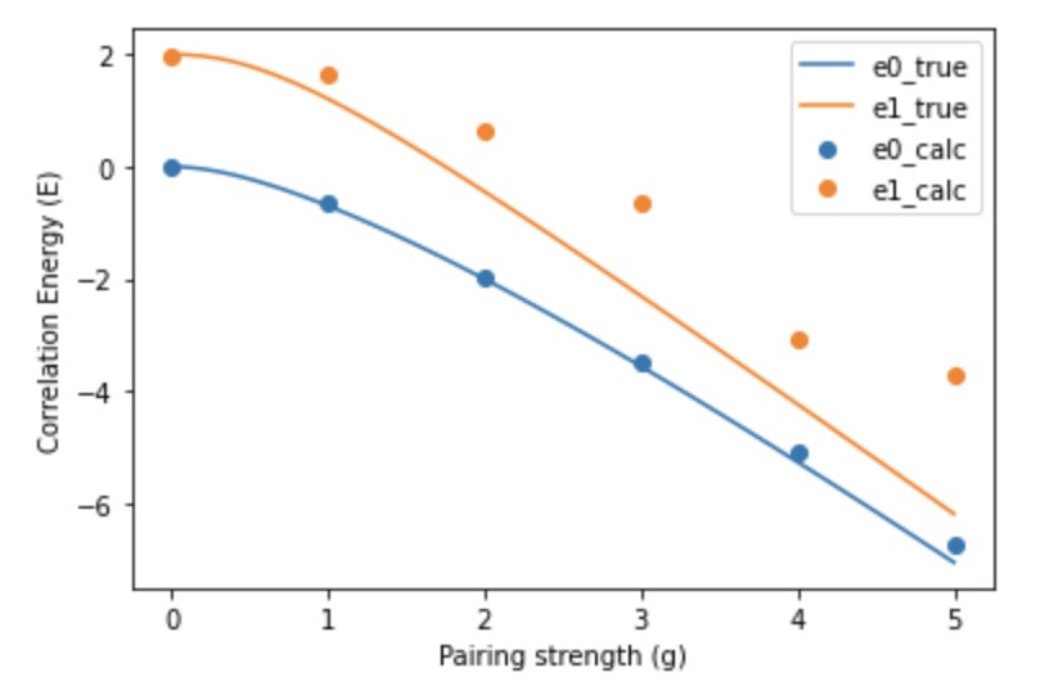
\includegraphics[scale=0.3]{excited states.jpg}
    \caption{Comparison of correlation energies calculated used in excited states algorithm vs direct diagonalization.}
    \label{fig:excited states}
\end{figure}

\subsection{Multi-Configuration Method}
\label{subsec:multi_conf}

We have observed that in the constant $g$ case, classical pCCD (and to a lesser but still significant extent) VQE with the UpCCD ansatz, have a harder and harder time finding the true ground state as $g$ grows. This is because the eigenfunction of the ground state becomes more and more entangled as $g$ grows and begins to overtake the strength of the single-particle energies $d_p$. Such entangled states heuristically take a larger circuit depth to employ.

Recall that the Dicke state \cite{ref:dicke} has the following recursive form
\begin{align}
\label{dicke_def}
\ket{D^n_k}
=
\sqrt{\frac{k}{n}}\ket{D^{n-1}_{k-1}}\ket{1}+\sqrt{\frac{n-k}{n}}\ket{D^{n-1}_k}\ket{0}
.\end{align}
We will now prove that the Dicke state $\ket{D^n_k}$ is an eigenvector of $V$ where
\begin{align}
V_n=g\sum_{p\neq q=1}^nA^\dagger_pA_q
.\end{align}
Specifically
\begin{align}
V_n\ket{D^n_k} 
=
gk(n-k)\ket{D^n_k}
.\end{align}
The proof is by induction. First, we prove the base case $(n,k)=(2,1)$.
\begin{align}
V_2\ket{D^2_1}
=
\frac{g}{\sqrt{2}}(A^\dagger_0A_1+A^\dagger_1A_0)(\ket{10}+\ket{01})
=
g\ket{D^2_1}
.\end{align}
Next, we assume the induction hypothesis
\begin{align}
V_n\ket{D^{n-1}_k} 
=
gk(n-k-1)\ket{D^{n-1}_k}
,\end{align}
and use it to prove the statement as follows
\begin{align}
V_n\ket{D^n_k}
&=
g
\left(\sum_{p\neq q=1}^nA^\dagger_pA_q\right)
\left(\sqrt{\frac{k}{n}}\ket{D^{n-1}_{k-1}}\ket{1}+\sqrt{\frac{n-k}{n}}\ket{D^{n-1}_k}\ket{0}\right)
\\
&=
g
\left[
\sum_{p\neq q=1}^{n-1}A^\dagger_pA_q
+
A^\dagger_n\left(\sum_{q=1}^{n-1}A_q\right)
+
\left(\sum_{p=1}^{n-1}A^\dagger_p\right)A_n
\right]
\nonumber
\\
& \hspace{3.5mm} \times
\left[\sqrt{\frac{k}{n}}\ket{D^{n-1}_{k-1}}\ket{1}+\sqrt{\frac{n-k}{n}}\ket{D^{n-1}_k}\ket{0}\right]
\\
&=
g
\left(\sum_{p\neq q=1}^{n-1}A^\dagger_pA_q\right)
\left(\sqrt{\frac{k}{n}}\ket{D^{n-1}_{k-1}}\ket{1}+\sqrt{\frac{n-k}{n}}\ket{D^{n-1}_k}\ket{0}\right)
\nonumber
\\
&+
g
\left[
A^\dagger_n\left(\sum_{q=1}^{n-1}A_q\right)
\sqrt{\frac{n-k}{n}}\ket{D^{n-1}_k}\ket{0}
+
\left(\sum_{p=1}^{n-1}A^\dagger_p\right)A_n
\sqrt{\frac{k}{n}}\ket{D^{n-1}_{k-1}}\ket{1}
\right]
\\
&=
(k-1)(n-k)\sqrt{\frac{k}{n}}\ket{D^{n-1}_{k-1}}\ket{1}
+
k(n-k-1)\sqrt{\frac{n-k}{n}}\ket{D^{n-1}_k}\ket{0}
\nonumber
\\
&+
(n-k)\sqrt{\frac{k}{n}}\ket{D^{n-1}_{k-1}}\ket{1}
+
k\sqrt{\frac{n-k}{n}}\ket{D^{n-1}_k}\ket{0}
\\
&=
k(n-k)\left(\sqrt{\frac{k}{n}}\ket{D^{n-1}_{k-1}}\ket{1}+\sqrt{\frac{n-k}{n}}\ket{D^{n-1}_k}\ket{0}\right)
\\
&=
k(n-k)\ket{D^n_k}
.\end{align}
In this proof we have used the following lemmas:
\begin{align}
\sum_{p=1}^nA^\dagger_p\ket{D^n_k}
&=\sqrt{n-k}\sqrt{k+1}\ket{D^n_{k+1}},
\\
\sum_{p=1}^nA\ket{D^n_k}
&=\sqrt{n-k+1}\sqrt{k}\ket{D^n_{k-1}},
\end{align}
which themselves are proven inductively in Appendix \ref{app:dicke_state_lemmas}. 

We can see how close the actual ground state of the pairing model (with $d_p=p$) is to the Dicke state for various values of $g$ by plotting their overlap squared. In Figure \ref{fig:pairing_dicke_overlap_pic}) we see such a plot for various energy levels $p$ (with $n=\lfloor p/2 \rfloor$). The plot shows that by the time $g$ reaches about 2.5, the overlap squared of the two states is above $0.9$ for all values of $p$ considered. It is also clear that the ground states for smaller values of $p$ become closer to the Dicke state $\ket{D^p_n}$ at a faster rate than for larger values of $p$.

\begin{figure}
    \centering
    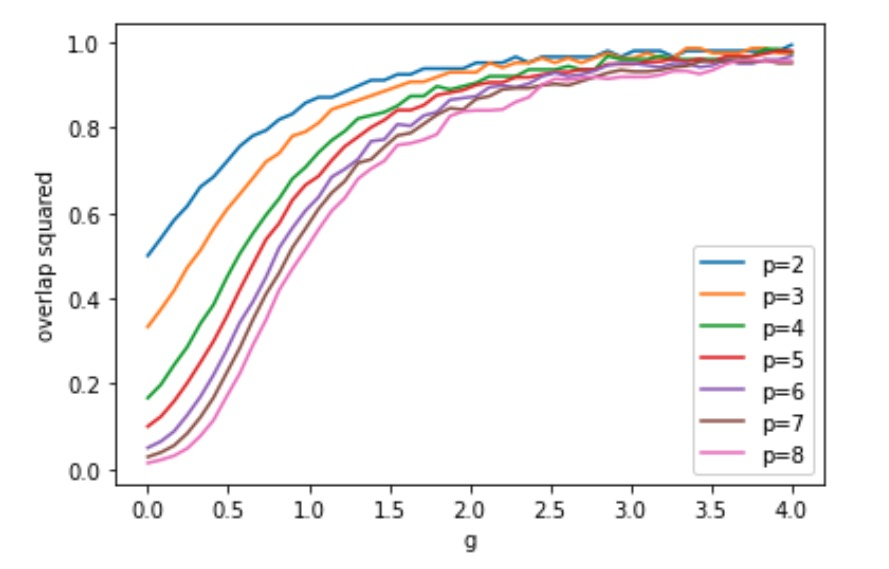
\includegraphics[scale=0.35]{pairing_dicke_overlap_pic.jpg}
    \caption{Plot of overlap squared between actual ground state and Dicke state for pairing models with various values of $p$ and $n=\lfloor p/2 \rfloor$ over increasing values of pairing strength.}
    \label{fig:pairing_dicke_overlap_pic}
\end{figure}

This suggests that, for sufficiently large $g$, one might consider the following ansatz for the pairing model. Use the deterministic \cite{ref:dicke_prep} or variational (chapter \ref{chap:vpds}) method to initialize one's quantum circuit to the Dicke state $\ket{D^p_n}$ for a pairing model with $p$ energy levels and $n$ pairs of fermions. Then, slowly increase the number of layers of variational gates in a "brick wall" fashion (\ref{brickwall}), running VQE on the ansatz each time, until the result no longer improves substantially. This is a so-called "adaptive" ansatz as it can change throughout the process of VQE. We tested such an ansatz, whose circuit representation is given below
\begin{align}
\Qcircuit @C=1em @R=1em
{
\lstick{\ket{0}} & \multigate{3}{U^4_2} & \multigate{1}{A(\theta_0)}  & \qw & \qw
\\
\lstick{\ket{0}} & \ghost{U^4_2}        & \ghost{A(\theta_0)} & \multigate{1}{A(\theta_2)} & \qw
\\
\lstick{\ket{0}} & \ghost{U^4_2}        & \multigate{1}{A(\theta_1)} & \ghost{A(\theta_2)} & \qw 
\\
\lstick{\ket{0}} & \ghost{U^4_2}        & \ghost{A(\theta_1)} & \qw & \qw
}
\end{align}
where the gate $U^4_2$ prepares the corresponding Dicke state:
\begin{align}
U^4_2\ket{0000}=\ket{D^4_2},
\end{align}
and $A$ is defined the same as the two-qubit operators for the UpCCD ansatz (\ref{aia}) except that the their parameters $\theta_i$ (for $i=0,1,2$) are completely free. That is
\begin{align}
A(\theta)=\exp\left\{i\theta(X_aY_i-Y_aX_i)\right\},
\end{align}
which, as analyzed previously, restricts the minimization algorithm's search to the correct Hamming weight subspace. The results of using such an ansatz for VQE can be seen in Figures \ref{fig:pairing_dicke_e_pic} and \ref{fig:pairing_dicke_error_pic}. The first shows a comparison between the VQE estimated and exact correlation energies while the second shows the relative error between the two from the first plot. As expected, this multi-configuration ansatz described above works better for larger absolute values of $g$, because we start in a state (the Dicke state) that has a significant overlap with the ground state. We name the ansatz this as it's initialized to the superposition of multiple initial configurations of the fermion pairs (or, bit-string states).

\begin{figure}
    \centering
    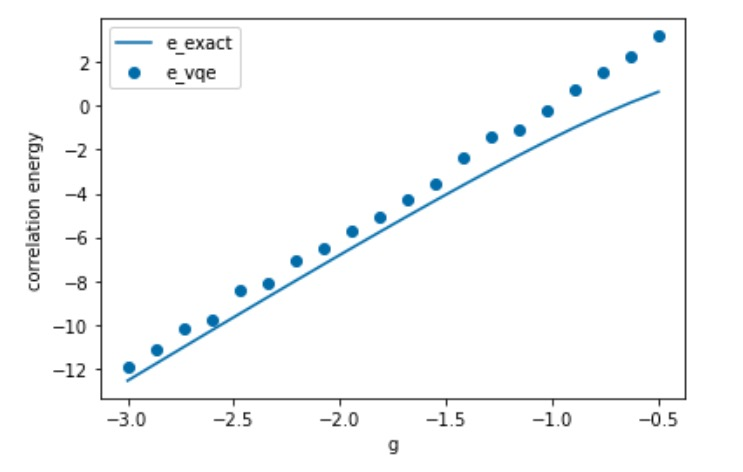
\includegraphics[scale=0.35]{pairing_dicke_e_pic.jpg}
    \caption{Plot of VQE estimated versus exact correlation energies for the pairing model ($(p,n)=(4,2)$) using the multi-configuration ansatz.}
    \label{fig:pairing_dicke_e_pic}
\end{figure}

\begin{figure}
    \centering
    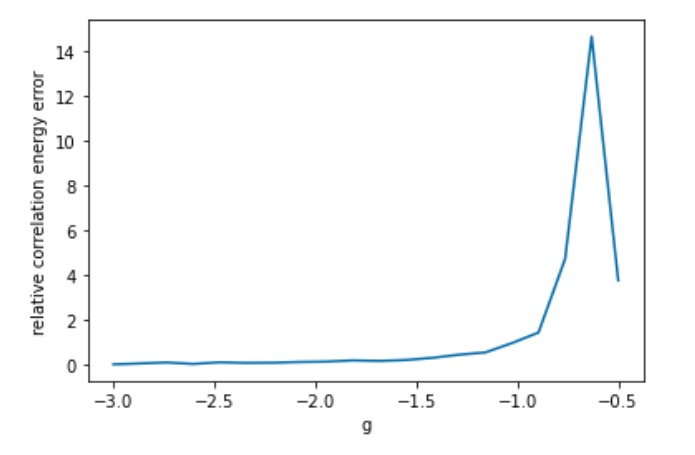
\includegraphics[scale=0.35]{pairing_dicke_error_pic.jpg}
    \caption{Plot of relative error between VQE estimated and exact correlation energies for the pairing model ($(p,n)=(4,2)$) using the multi-configuration ansatz.}
    \label{fig:pairing_dicke_error_pic}
\end{figure}

In future work, it would be of interest to explore if one can get away with preparing a Dicke like state (equal superposition of bit-string states but with incorrect phases, such as those prepared in chapter \ref{chap:vpds}) or even partial Dicke states (the equal superposition of some of the bit-string states that make up an entire Dicke states). One could also explore this ansatz for a larger number of energy levels $p$ and different formulas of the single particle energies $d_p$. Finally, on might consider using the first few layers of the UpCCD ansatz to try to minimize the pairing model with $d_p=0$ which should get one close to a Dicke state. Then add in the rest of the layers and minimize to the pairing model that one desires, however, initializing the initial layers to the parameters that the minimization algorithm found approximated the Dicke state. 

\section{Conclusion}

In this section, we introduce the pairing model, a toy model for many-body nuclear physics upon which many new techniques are tested. First, we explored ways to solve the problem on a classical computer, including through many-body perturbation theory and coupled cluster theory. These two methods served to help us in the next section to inform a good set of initial guesses for our variational circuit. In the aforementioned section, we walked through how to map the pairing model Hamiltonian and an extension of the unitary coupled cluster ansatz from fermionic operators to spin operators via an extension to the Jordan-Wigner transformation . We then presented our results of applying VQE to the pairing model and bench-marked it against classical coupled cluster theory. We then went on to extend VQE in two novel ways: first, we introduced the novel iterative quantum excited state algorithm to search for the energy levels of excited states of the pairing model. Then we introduced the novel multi-configurational ansatz for pairing models with large pairing strengths $g$. In the future, one might like to compare our excited states algorithms to other such algorithms and also test various relaxed forms of the multi-configurational ansatz that involve the initialization of Dicke-like states. Finally, one may wish to apply the VQE solution to the pairing problem to approximate an actual nucleus that has strong pairing interactions such as ones with doubly-magic shells with valence electrons of a single type. Here, we have given a springboard off of which future research can be accomplished as quantum computing tackles more and more complex many-body nuclear physics systems.

\chapter{Collective Neutrino Oscillations}

\nocite{ref:cno}

\section{Introduction}

The next system we will consider is that of collective neutrino oscillations. It has a Hamiltonian that is mathematically identical to that of the previous pairing models considered. Instead of using quantum algorithms to determine the solution to the Hamiltonian (energy eigenvalues), as done in the two previous cases, we will instead use them to simulate the time-evolution of the system and measure its entanglement properties. Neutrinos are nuclear particles in the sense that they interact via the weak nuclear force (and gravity). The motivation for studying this system comes from the flavor evolution of neutrinos in dense astrophysical environments have. It has been pointed out by Pantelone, Raffelt, and Sigl~\cite{Pantaleone:1992eq,Sigl:1993} and others that neutrinos can exchange their flavors, through forward scattering. If one starts with an anisotropic initial distribution in energy and/or angle (as found in supernovae, neutron star mergers, or the early universe), then the neutrino energy flux versus energy and flavor may be impacted by this non-trivial quantum many-body evolution. This can in turn affect the dynamics of these environments and other observable signatures, including nucleosynthesis in the ejected material (see~\cite{Duan:2010bg,Chakraborty2016b} for recent reviews).

Most often these quantum equations have been treated on the mean-field level by replacing one of the spin operators in equation \eqref{eq:fws_int} by its expectation value, yielding a set of non-linear coupled differential equations. This makes the calculations tractable for several hundred energies and angles on modern computers (see eg.~\cite{Duan:2006}).
More recently, studies of neutrino propagation as a quantum many-body problem have appeared,
including for example \cite{Bell2003,Friedland2003,sawyer2004classical,Pehlivan2011,Rrapaj2020,Cervia:2019,Roggero2021a,Roggero2021b}. These works highlight the importance of understanding the role of quantum correlations, such as entanglement, in order to quantify beyond mean-field effects in out-of-equilibrium neutrino simulations. A direct solution of the Schr\"{o}dinger equation in equation \eqref{eq:schroedinger-eq}, for a system of $N$ configurations in energy and angle, incurs a computational cost that is exponential in $N$. This has limited early explorations of the problem to systems with $N=\mathcal{O}(10)$ neutrinos. An alternative to reach larger system sizes, explored recently by one of us in Refs.~\cite{Roggero2021a,Roggero2021b}, employs a Matrix Product State representation for $\ket{\Phi(t)}$ which allows one to track the exact time evolution in situations where entanglement never grows too much. For conditions leading to strong entanglement instead, simulations on digital/analog quantum computers have the potential to tackle the full neutrino dynamics while still enjoying a polynomial computational cost in system size $N$~\cite{Lloyd96}.

In this section we explore the time-dependent many-body evolution and entanglement of neutrinos on a current-generation digital quantum computer. In section \ref{sec:spin_model} we introduce in more detail the SU(2) spin model used to describe collective neutrino oscillations and describe an implementation of the time evolution operator appearing in equation \eqref{eq:schroedinger-eq} suitable for an array of qubits with linear connectivity. We present the results obtained for a a small system with $N=4$ neutrino amplitudes in section \ref{sec:real_time} and provide a summary and conclusions in section \ref{sec:conclusion}.

\section{Hamiltonian}
\label{sec:spin_model}

The Hamiltonian for neutrino flavor evolution in a dense neutrino environment includes three terms: 
\begin{enumerate}
    \item $H_v$ | the vacuum mixing that has been determined from solar and accelerator neutrino experiments~\cite{GonzalezGarcia:2003}
    \item $H_s$ | the forward scattering in matter leading to the well known MSW effect~\cite{Wolfenstein:1977ue,Mikheev:1986gs}
    \item $H_n$ | neutrino-neutrino forward scattering
\end{enumerate}

The first simplification we make is to truncate the neutrino flavors involved from three to two. That is, we only consider the oscillation of two flavors which, without loss of generality, we choose to be $\nu_e$ and $\nu_x$. Here $\nu_x$ describes the $\nu_\mu$ and $\nu_\tau$ flavors which we assume evolve similarly. This simplification allows for the neutrino-neutrino interaction $H_n$ to be proportional to the dot product ${\sigma}_i \cdot {\sigma}_j$ of the SU(2) Pauli matrices
describing the different flavor amplitudes of the two neutrinos
\begin{equation}
\label{eq:fws_int}
(H_n)_{ij}\propto \left(1-\frac{{q}_i\cdot{q}_j}{\|{q}_i\|\|{q}_j\|}\right){\sigma}_i\cdot{\sigma}_j\;.
\end{equation}
where ${q}_k$ is the momentum of the $k$-th neutrino and ${\sigma}_k=(X_k,Y_k,Z_k)$ is the vector of Pauli operators acting on its amplitude. The neutrino-neutrino interaction can exchange
flavors of two neutrinos and, as can be seen above, has a forward scattering amplitude that depends on the angle between their momenta. Generalization to the three-flavor case is straightforward in principle. We are working in the neutrino flavor basis, whose fermionic operators are related to those of the mass basis via the rotation
\begin{align}
\label{flavor_mass_rotation}
\begin{pmatrix}
a_e(p) \\ a_x(p)
\end{pmatrix}
=
\begin{pmatrix}
\cos\theta & \sin\theta \\
-\sin\theta & \cos\theta 
\end{pmatrix}
\begin{pmatrix}
a_1(p) \\ a_2(p)
\end{pmatrix}
.\end{align}
In this basis the vacuum term $H_v$ includes diagonal contributions describing the mass differences between different neutrino flavors and an off-diagonal term characterized by a mixing angle $\theta_v$, while forward scattering term $H_s$ is diagonal in the flavor basis.

For the simplified two-flavor case studied here, the state of the system can be described an amplitude for a neutrino of each energy $E_i$ (equal to the magnitude of momentum $\|{q}_i\|$) and direction of momentum (denoted by $q_i$), with $\alpha_\uparrow$ and $\alpha_\downarrow$ describing the amplitude of being in the electron flavor or in a heavy $x$ ($\mu$ or $\tau$) flavor respectively. These two amplitudes can be encoded in an SU(2) spinor
basis. In this basis, the Hamiltonian can be written in terms of Pauli operators as the sum of a one-body term, describing both vacuum oscillations and forward scattering in matter, 
\begin{equation}
\label{eq:Ham_init}
H_1  = \frac{1}{2} \sum_i \left[ \left(-\Delta_i\cos{2 \theta_v} + A\right)\sigma^z_i + \Delta_i\sin {2 \theta_v} \sigma^x_i \right]\;,
\end{equation}
and a two-body term, coming from the neutrino-neutrino forward-scattering potential $V_{ij}$ from equation \eqref{eq:fws_int}, which takes the following form~\cite{Pehlivan2011}
\begin{equation}
\begin{split}
H_2 & =  \sum_{i<j} \eta  [1- \hat{q}_i \cdot \hat{q}_j ] \vec{\sigma}_i \cdot \vec{\sigma}_j\;.
\end{split}
\end{equation}
%where we denoted by $\vec{\sigma}_k=(\sigma_k^x,\sigma_k^y,\sigma_k^z)$ the vector of Pauli operators.
In the one-body term, $\theta_v$ represents the vacuum mixing angle, while the strength is given by $\Delta_i = \delta m^2/(2 E_i)$ with $\delta m^2$ the mass squared difference for neutrinos of different flavor. The matter potential enters as the diagonal contribution in the one-body term through the constant $A = \sqrt{2} G_F n_e$, with $G_F$ the Fermi coupling constant and $n_e$ the electron density.

As described in the introduction, the two-body term is a sum over spin-spin interactions with a coupling depending upon the relative angle between them. The overall strength depends on the neutrino density as
\begin{equation}
\label{eq:eta}
\eta=\frac{G_F}{\sqrt{2}V}=\frac{G_F n_\nu}{\sqrt{2}N}\;,
\end{equation}
with $N$ the number of neutrino momenta considered, given by the neutrino density $n_\nu$ times the quantization volume $V$. We can transform from fermionic flavor operators to flavor isospin operators via the Jordan-Schwinger mapping:
\begin{align}
\label{flavor_fermionic_to_isospin_jp}
J^+_p&=a^\dagger_e(p)a_x(p),
\\
\label{flavor_fermionic_to_isospin_jm}
J^-_p&=a^\dagger_x(p)a_e(p),
\\
\label{flavor_fermionic_to_isospin_jz}
J^z_p&=\frac{1}{2}\left(a^\dagger_e(p)a_e(p)-a^\dagger_x(p)a_x(p)\right)
,\end{align}
which obey the SU(2) commutation relations
\begin{align}
\comm*{J^+_p}{J^-_q}&=2\delta_{pq}J^z_p
\\
\comm*{J^z_p}{J^{\pm}_q}&=\pm\delta_{pq}J^{pm}_p
,\end{align}
and are thus isomorphic to the Pauli-spin matrices. Note that we can transform to Cartesian coordinates through the definition
\begin{align}
J^\pm_p=J^x_p\pm iJ^y_p
\end{align}
The term of the Hamiltonian that describes vacuum oscillations $H_\nu$ is given by
\begin{align}
\label{vacuum_oscillation_term}
H_\nu = \sum_{p}\left(\frac{m_1^2}{2p}a^\dagger_1(p)a_1(p)+\frac{m_2^2}{2p}a^\dagger_2(p)a_2(p)\right)
,\end{align}
in the mass basis. To transform it to the Pauli basis, we first subtract it by the following term
\begin{align}
\sum_p\frac{m_1^2+m_2^2}{4p}\left(a^\dagger_1(p)a_1(p)+a^\dagger_2(p)a_2(p)\right)
,\end{align}
which can be done without consequence as it is proportional to the identity (for a given number of particles) since the total number of neutrinos in each momentum mode is constant. (This follows from the fact that forward scattering only exchanges the neutrino's momenta.) Subtracting said term transforms the vacuum oscillation term (\ref{vacuum_oscillation_term}) into
\begin{align}
\label{vacuum_oscillation_term2}
H_\nu = \sum_p\frac{\Delta m^2}{4p}\left(a^\dagger_2(p)a_2(p)-a^\dagger_1(p)a_1(p)\right)
,\end{align}
where $\Delta_m^2=m_2^2-m_1^2$. Applying the inverse of the mapping between the flavor and mass bases (\ref{flavor_mass_rotation}) yields
\begin{align}
H_\nu
&=
\sum_p\frac{\Delta m^2}{4p}\Big{[}
(\sin\theta a^\dagger_e(p)+\cos\theta a^\dagger_x(p))\left(\sin\theta a_e(p)+\cos\theta a_x(p)\right)
\nonumber
\\
&\hspace{17.5mm}-
(\cos\theta a^\dagger_e(p)-\sin\theta a^\dagger_x(p))\left(\cos\theta a_e(p)-\sin\theta a_x(p)\right)
\Big{]}
\\
&=
\sum_p\frac{\Delta m^2}{4p}\Big{[}
\sin2\theta\left(a^\dagger_e(p)a_x(p)+a^\dagger_x(p)a_e(p)\right)
\nonumber 
\\
&\hspace{18mm}-
\cos2\theta\left(a^\dagger_e(p)a_e(p)-a^\dagger_x(p)a_x(p)\right)
\Big{]}
,\end{align}
which can be mapped to the Pauli basis via (\ref{flavor_fermionic_to_isospin_jp})-(\ref{flavor_fermionic_to_isospin_jz}), resulting in
\begin{align}
\label{neutrino_neutrino_interaction}
H_\nu = \sum_p B\cdot \sigma_p
,\end{align}
where
\begin{align}
B=\frac{\Delta m^2}{2p}(\sin2\theta,0,-\cos2\theta).
\end{align}
We've written the Hamiltonian in terms of Paul operators instead of the SU(2) operators $J^\pm$ and $J^z$ as the two are isomorphic. The neutrino-neutrino scattering term is given by
\begin{align}
H_{\nu\nu}
&=
\frac{G_F}{\sqrt{2}V}\sum_{pq}(1-\cos\phi_{pq})
\big{[}
a^\dagger_e(p)a_x(p)a^\dagger_x(q)a_e(q)+a^\dagger_x(p)a_e(p)a^\dagger_e(q)a_x(q)
\nonumber
\\
&\hspace{41.5mm}+
a^\dagger_e(p)a_e(p)a^\dagger_e(q)a_e(q)+a^\dagger_x(p)a_x(p)a^\dagger_x(q)a_x(q)
\big{]}
,\end{align}
which can be mapped to the Pauli basis via (\ref{flavor_fermionic_to_pauli_mapping}), resulting in
\begin{align}
\label{neutrino_neutrino_term2}
H_{\nu\nu}
&=
\frac{G_F}{\sqrt{2}V}\sum_{pq}(1-\cos\phi_{pq})
\left(
\sigma^+_p\sigma^-_q+\sigma^-_q\sigma^+_p + \sigma^z_p\sigma^z_q
\right)
\nonumber
\\
&=
\sum_{pq}J_{pq}
\sigma_p\cdot\sigma_q
,\end{align}
with
\begin{align}
J_{pq}=\frac{\sqrt{2}G_F}{V}(1-\cos\phi_{pq})
,\end{align}
where we've disregarded the term $a_e^\dagger(p)a_e(p)a_x^\dagger(q)a_x(q)+a_x^\dagger(p)a_x(p)a_e^\dagger(q)a_e(q)$ as it is proportional to the identity. Note that this is in terms of Pauli spin matrices as opposed to angular momentum operators but they are isomorphic as they obey the same SU(2) commutation relations. Putting the two terms together, the Hamiltonian for collective neutrino oscillations becomes
\begin{align}
\label{cno_hamiltonian}
H=\sum_pB\cdot\sigma_p+\sum_{p<q}J_{pq}\sigma_p\cdot\sigma_q
,\end{align}
where we're able to restricted to sum to $p<q$ as the $p=q$ term is proportional to the identity and restricting $p\neq q$ to $p<q$ only picks up a factor of two which can be absorbed into the constant $J_{pq}$. We note that the Hamiltonian is similar to the Heisenberg model except that the two-body term is all-to-all rather than nearest neighbor; that is, it sums over both $p$ and $q$ rather than summing over $p$ and $p+1$. Its coupling strength $\eta\propto1/N$ assures that the energy of the system is extensive. This allows us to obtain a well-defined many-body solution, in the limit of large
numbers of neutrino momenta by extrapolating in system size $N$.

Because NISQ-era quantum computers must have a relatively limited circuit depth in order to not be too noisy 
%\cite{Preskill2018}
the maximum time to which we can simulate time-evolution is also limited. Therefore, we consider a test case where the one-body and two-body interaction terms set to be similar in magnitude, allowing flavor oscillations to occur rapidly. An example of this case is the environment of order $\approx100$ km from the surface of a proto-neutron star in a core collapse supernovae. Here the background matter density has decreased to the point where its contribution to the Hamiltonian is similar in magnitude to the neutrino-neutrino forward scattering. The relative angles of neutrino propagation are fairly small as neutrinos are emitted from a typical proto-neutron star radius of order 10 km. In the neutrino bulb model~\cite{Duan:2006} one further assumes the evolution in a supernovae depends only on the energy and the angle from the normal. Averaging over the azimuthal angles results in an average
coupling $\langle 1-{\hat {q}}_i \cdot {\hat {q}}_j \rangle = 1 - \cos(\theta_i) \cos(\theta_j).$
% Often a further simplification, usually called single-angle approximation, is made where an average coupling is taken between all pairs of neutrinos, resulting in a two-body term simply related to the square of the total spin $S$ of the many-body state.

For our test case, we take a monochromatic neutrino beam with energy $E_\nu=\delta m^2/(4\eta)$ and measure energies in units of the two-body coupling $\eta$. In order to avoid the symmetries introduced by the single angle approximation, we employ an anisotropic distribution of momentum directions
using a simple grid of angles with
\begin{equation}
\phi_{pq} = \arccos(0.9) \frac{|p-q|}{N-1}\;.
\end{equation}
This is similar to the standard bulb model as the relative couplings $1- \cos\phi_{pq}$ are small. Additionally, we choose $\theta=0.195$ so that the one-body and two-body terms are of relative strength. This leads the parameters to have the following numerical values:
\begin{align}
B&=\left(\sqrt{1-0.925^2},0,-0.925\right)
\\
J_{pq}&=\left[1-\cos\left(\arccos{0.9}\frac{\abs{p-q}}{N-1}\right)\right]
.\end{align}

\section{Connection to the Pairing Model}

Before we go any further, we'd like to show here how collective neutrino oscillations can be viewed as a pairing model, thus justifying its use as an application of the pairing model. This connection can be seen by writing the collective neutrino oscillation Hamiltonian in the mass basis. To do so, we introduce the
mass isospin operators
\begin{align}
K^+_p&=a^\dagger_1(p)a_2(p)
\\
K^-_p&=a^\dagger_2(p)a_1(p)
\\
K^z_p&=\frac{1}{2}\left(a^\dagger_1(p)a_1(p)-a^\dagger_2(p)a_2(p)\right)
,\end{align}
which are analogous to the flavor isospin operators (\ref{flavor_fermionic_to_isospin}). This allows the vacuum oscillation term (\ref{vacuum_oscillation_term2}) to be readily identified as
\begin{align}
\label{vacuum_oscillation_term_k}
H_\nu 
&= 
\sum_p\frac{\Delta m^2}{4p}\left(a^\dagger_2(p)a_2(p)-a^\dagger_1(p)a_1(p)\right)
\nonumber
\\
&=
\sum_p\omega_pK^z_p
,\end{align}
where
\begin{align}
\omega=-\frac{\Delta m^2}{2p}
.\end{align}
In order to deal with the neutrino neutrino interaction term (\ref{neutrino_neutrino_interaction}), we must find the mapping the transformation between flavor isospin operators and mass isospin operators which follows from the mapping between flavor fermionic operators and mass fermionic operators (\ref{flavor_mass_rotation}) as
\begin{align}
J^+_p
&=
a^\dagger_e(p)a_x(p)
\nonumber
\\
&=
[\cos\theta a^\dagger_1(p)+\sin\theta a^\dagger_2(p)]
[\cos\theta a_2(p)-\sin\theta a_1(p)]
\nonumber
\\
&=
\cos^2\theta a^\dagger_1(p)a_2(p)-\sin^2\theta a_2^\dagger(p)a_1(p)-\frac{1}{2}\sin2\theta[a^\dagger_1(p)a_1(p)-a^\dagger_2(p)a_2(p)]
\nonumber
\\
&=
\cos^2\theta K^+_p-\sin^2\theta K^-_p-\sin2\theta K^z,
\\
J^-_p
&=
a^\dagger_e(p)a_x(p)
\nonumber
\\
&=
[\cos\theta a^\dagger_2(p)-\sin\theta a^\dagger_1(p)]
[\cos\theta a_1(p)+\sin\theta a_2(p)]
\nonumber
\\
&=
\cos^2\theta a_2^\dagger(p)a_1(p)
-
\sin^2\theta a^\dagger_1(p)a_2(p)
-
\frac{1}{2}\sin2\theta[a^\dagger_1(p)a_1(p)-a^\dagger_2(p)a_2(p)]
\nonumber
\\
&=
\cos^2\theta K^-_p-\sin^2\theta K^+_p-\sin2\theta K^z,
\\
J^z_p
&=
\frac{1}{2}\left(a^\dagger_e(p)a_e(p)-a^\dagger_x(p)a_x(p)\right)
\nonumber
\\
&=
\frac{1}{2}
\{
[
\cos\theta a^\dagger_1(p)+\sin\theta a^\dagger_2(p)
]
\left[
\cos\theta a_1(p)+\sin\theta a_2(p)
\right]
\nonumber
\\
&\hspace{5.5mm}-
[
\cos\theta a^\dagger_2(p)-\sin\theta a^\dagger_1(p)
]
\left[
\cos\theta a_2(p)-\sin\theta a_1(p)
\right]
\}
\nonumber
\\
&=
\frac{1}{2}
\{
\cos2\theta[a^\dagger_1(p)a_1(p)-a^\dagger_2(p)a_2(p)]
+
\sin2\theta[a^\dagger_1(p)a_2(p)-a^\dagger_2(p)a_1(p)]
\}
\nonumber
\\
&=
\cos2\theta K^z_p+\frac{1}{2}\sin2\theta(K^+_p+K^-_p)
,\end{align}
which can be expressed succinctly in matrix form, for reference, as
\begin{align}
\begin{pmatrix}
J^+_p \\ J^-_p \\ J^z_p
\end{pmatrix}
=
\begin{pmatrix}
\cos^2\theta & -\sin^2\theta & -\sin2\theta \\
-\sin^2\theta & \cos^2\theta & -\sin2\theta \\
\frac{1}{2}\sin2\theta & \frac{1}{2}\sin2\theta & \cos2\theta
\end{pmatrix}
\begin{pmatrix}
K^+_p \\ K^-_p \\ K^z_p
\end{pmatrix}
.\end{align}
This implies that the dot product of the total flavor isospin operators is
\begin{align}
J_p\cdot J_q
&=
\frac{1}{2}
(J^+_pJ^-_q+J^-_pJ^+_q)+J^z_pJ^z_q
\nonumber
\\
&=
\frac{1}{2}
\begin{pmatrix}
J^+_p & J^-_p & J^z_p
\end{pmatrix}
\begin{pmatrix}
J^-_p 
\\ 
J^+_p 
\\ 
2J^z_p
\end{pmatrix}
\nonumber
\\
&=
\frac{1}{2}
\begin{pmatrix}
K^+_p & K^-_p & K^z_p
\end{pmatrix}
\begin{pmatrix}
\cos^2\theta & -\sin^2\theta & \frac{1}{2}\sin2\theta \\
-\sin^2\theta & \cos^2\theta & \frac{1}{2}\sin2\theta \\
-\sin2\theta & -\sin2\theta & \cos2\theta
\end{pmatrix}
\begin{pmatrix}
\cos^2\theta & -\sin^2\theta & -\sin2\theta \\
-\sin^2\theta & \cos^2\theta & -\sin2\theta \\
\sin2\theta & \sin2\theta & 2\cos2\theta
\end{pmatrix}
\begin{pmatrix}
K^-_p 
\\ 
K^+_p 
\\ 
K^z_p
\end{pmatrix}
\nonumber
\\
&=
\frac{1}{2}
\begin{pmatrix}
K^+_p & K^-_p & K^z_p
\end{pmatrix}
\begin{pmatrix}
1 & 0 & 0 \\
0 & 1 & 0 \\
0 & 0 & 2
\end{pmatrix}
\begin{pmatrix}
K^-_p 
\\ 
K^+_p 
\\ 
K^z_p
\end{pmatrix}
\nonumber
\\
&=
\frac{1}{2}
(K^+_pK^-_q+K^-_pK^+_q)+K^z_pK^z_q
\\
&=
K_p\cdot K_q
,\end{align}
equal to the dot product of the total mass isospin operators. This means that the neutrino-neutrino interaction term (\ref{neutrino_neutrino_term2}) can be written in terms of total mass isospin operators as 
\begin{align}
\label{neutrino_neutrino_term_k}
H_{\nu\nu}=\sum_{pq}J_{pq}K_p\cdot K_q
.\end{align}
Putting the terms (\ref{vacuum_oscillation_term_k} - \ref{neutrino_neutrino_term_k}) together gives us the Hamiltonian in terms of mass isospin operators
\begin{align}
H=\sum_p\omega_pK^z_p+\sum_{pq}J_{pq}K_p\cdot K_q
.\end{align}
Consider now the single-angle approximation, where we assume that neutrinos traveling in different directions undergo the same flavor evolution, implying that the term $\sum_{pq}\cos\phi_{pq}J_p\cdot J_q$ (and therefore also $\sum_{pq}\cos\phi_{pq}K_p\cdot K_q$) averages to zero, which (after recalling $J_{pq}=\mu(1-\cos\phi_{pq})$) leads to the Hamiltonian
\begin{align}
H
&=
\sum_p\omega_pK^z_p+\mu\sum_{pq}K_p\cdot K_q
,\end{align}
which can be written as
\begin{align}
\label{neutrino_hamiltonian_saa}
H
&=
\sum_p\omega_pK^z_p+2\mu\sum_{p<q}(K^x_p\cdot K^x_q+K^y_p\cdot K^y_q)
,\end{align}
where we've dropped the terms $\mu\sum_{pq}K^z_p\cdot K^z_q$ and $\mu\sum_{p=q}(K^x_p\cdot K^x_q+K^y_p\cdot K^y_q)=2\mu\sum_{p}I_p$ as they are both proportional to the identity (for a fixed number of neutrinos) and therefore has no effect on the time-evolution of the system. Recall now the pairing Hamiltonian in terms of Pauli spin operators (\ref{pairing_model_hamiltonian_mapped}) which in the case of constant pairing strength ($g^p_q=g$) we can write as 
\begin{align}
\label{pairing_model_hamiltonian_compare}
H
=
-\frac{1}{2}\sum_{p=1}^P(2d_p+g)Z_p
+
\frac{1}{2}g\sum_{\substack{p,q=1 \\ p<q}}(X_pX_q+Y_pY_q)
,\end{align}
by dropping the term $\frac{1}{2}\sum_{p=1}^P(2d_p+g)I_p$ as it is proportional to the identity. With this, we can see that, since the mass isospin operators and Pauli-spin operators are isomorphic (share the same commutation relations), the collective neutrino oscillation Hamiltonian in the single-angle approximation (\ref{neutrino_hamiltonian_saa}) is equivalent (up to terms proportional to the identity) to pairing Hamiltonian with constant pairing strength (\ref{pairing_model_hamiltonian_compare})if we set $d_p=\omega_p-g/2$ and $g=4\mu$, implying that the two systems evolve identically in time.

\section{Time Evolution}
\label{sec:real_time}

The greatest challenge in implementing the time evolution of the collective neutrino oscillation Hamiltonian (\ref{cno_hamiltonian}) on a quantum computer is to find an accurate approximation to the time evolution operator (\ref{time_evolution_operator_definition})
\begin{align}
 U(t)=\exp\{-iHt\}  
,\end{align}
that can be decomposed efficiently into quantum gates (local unitary operators)\cite{Lloyd96}. Here, we do this by first using a first-order Trotter-Suzuki decomposition~\cite{Suzuki91} of the time evolution operator. This decomposition requires partitioning the Hamiltonian. The naive partitioning would be to simply keep the Hamiltonian (\ref{cno_hamiltonian}) written as is, which would lead to the following approximation for the time-evolution operator 
\begin{align}
\label{eq:trotter1}
U_1(t)=\prod_{p=1}^Ne^{-itB\cdot\sigma_p}\prod_{p<q=1}^Ne^{-it J_{pq}\sigma_p\cdot\sigma_q}
.\end{align}
However, we instead choose the pair propagation partition, in which we rewrite the Hamiltonian (\ref{cno_hamiltonian}) as a strictly two-body term
\begin{align}
\label{eq:ham_decomp}
H = \sum_{p<q}^N h_{pq}
,\end{align}
where
\begin{align}
h_{pq} = \frac{1}{N-1}B\cdot(\sigma_p+\sigma_q) + J_{pq}\sigma_p\cdot\sigma_q
,\end{align}
which we can do since
\begin{align}
\sum_{p<q}^n(\sigma_p+\sigma_q)
&=
\sum_{p=1}^n\sum_{q=p+1}^n(\sigma_p+\sigma_q) 
\nonumber 
\\
&=
\sum_{p=1}^n\sum_{q=p+1}^n\sigma_p+\sum_{q=2}^n\sum_{p=1}^{q-1}\sigma_q
\nonumber 
\\
&=
\sum_{p=1}^n(n-p)\sigma_p+\sum_{q=1}^n(q-1)\sigma_q
\nonumber 
\\
&=
\sum_{p=1}^n\left[(n-p)+(p-1)\right]\sigma_p 
\nonumber 
\\
&=(n-1)\sum_{p=1}^n\sigma_p
.\end{align}
This leads to the pair-propagation time-evolution operator approximation $U_2$, defined as
\begin{equation}
\label{eq:pair_prop_app}
U_2(t) = \prod_{p<q}^N u_{pq}
\end{equation}
where
\begin{align}
u_{pq} = e^{-ith_{pq}}
,\end{align}
which is correct up to additive error $\epsilon=\mathcal{O}(t^2)$.
This partitioning is motivated by past experience with the Euclidean version of this evolution operator in Quantum Monte Carlo which suggests that this partitioning yields a better approximation to the time-evolution operator $U(t)$ (see eg.~\cite{Ceperley1995,Carlson2015}). The main reason we choose this partitioning, however, is that it has better error scaling than the original partitioning $U_1$ 
as detailed below. While asymptotic scaling of the approximation error $\epsilon$ is quadratic in the time-step $t$ for both approximations~\cite{Suzuki91}, the pair approximation is expected to perform better in practice for cases where an accurate description of pair evolution is important due, for instance, to strong cancellations between the one-body and two-body contributions in the Hamiltonian. In the neutrino case, these situations can occur with appropriate initial conditions so that, for typical states in the evolution, we have for most pairs
\begin{equation}
\label{eq:pairp_err}
\left|\langle K_{pq}\rangle+\langle V_{pq}\rangle\right|\ll\left|\langle K_{pq}\rangle\right|+\left|\langle V_{pq}\rangle\right|
\end{equation}
where we used the short-hand
\begin{align}
\langle K_{pq}\rangle 
&=
\frac{1}{N-1}B\cdot\langle\sigma_p+\sigma_q\rangle
\\
\langle V_{pq}\rangle
&=
J_{pq}\langle\sigma_p\cdot\sigma_q\rangle
.\end{align}
Since the difference between the two approximations is not expected to hold for a generic initial state, standard error measures like the matrix norm of the difference with the exact propagator
\begin{equation}
\label{eq:mnorme}
\left\|\exp\left(-itH\right)-U_{1/2}(t)\right\|
\end{equation}
are not expected to capture the effect. This is, in fact, found in practice for our system. In panel (a) of Figure \ref{fig:prop_cmp} we show the estimate from equation \eqref{eq:mnorme} for the $N=4$ neutrino model considered in this work. This error estimate indicates that the $U_1$ approximation has a smaller maximum error than $U_2$ up to long times. We can look at a more direct measure of accuracy for our specific setup by considering instead the state fidelity 
\begin{equation}
f(t) = \left|\langle \Psi_{1,2}(t)|\Psi(t)\rangle\right|^2   
\end{equation}
between the exact state $\ket{\Psi(t)}$ at time $t$ and one of its approximations $\ket{\Psi_{1,2}(t)}$, defined as
\begin{align}
\ket{\Psi_{1,2}(t)}=U_{1,2}\ket{\Psi(0)}
.\end{align}
We show $f(t)$ for both approximations in panel (b) of Figure \ref{fig:prop_cmp}. The result here suggest that instead the pair approximation produces a state with a higher fidelity than the simple linear propagator $U_1$, especially at relatively long time-steps $t\in[4,8]$.

\begin{figure}[h]
\centering
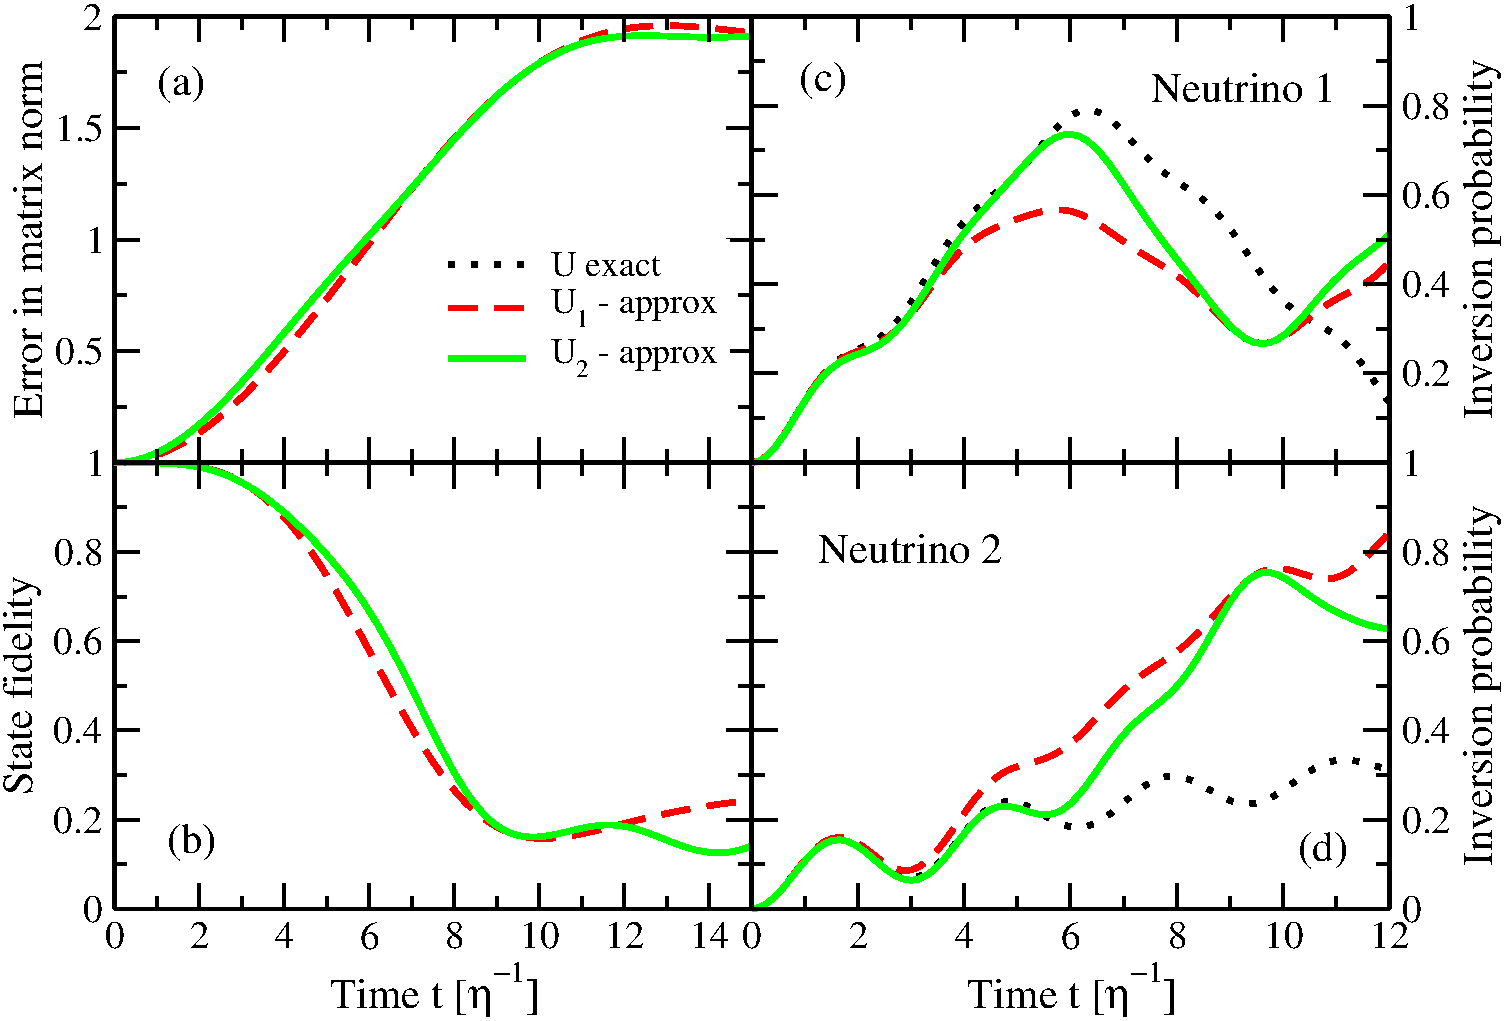
\includegraphics[width=0.7\textwidth]{prop_plot.pdf}
\caption{(Color online) Panel (a) shows the error in matrix 2-norm equation \eqref{eq:mnorme} of the two approximations $U_1$ and $U_2$ described in the text. Panel (b) shows the state fidelity and the right panels show results for the inversion probability $P_{\text{inv}}(t)$. Panel (c) is for neutrino one while panel (d) is for neutrino 2.}
\label{fig:prop_cmp}
\end{figure}

Finally, since we are mostly interested in flavor observables diagonal in the computational basis, we also show a direct comparison of the inversion probability for two out of the $N=4$ neutrinos using both approximations and the exact propagator (panels (c) and (d)). The details of how we compute the inversion probability is forthcoming but these selected results were included here first to show more clearly that the pair approximation allows us to correctly describe the evolution of flavor for substantially longer times than the $U_1$ approximation. The results reported here do depend on the specific choice of ordering of qubits in the time evolution layers shown in Figure \ref{fig:swap_network}. In both the present analysis and the simulation results we used the best ordering which we empirically found to be $(1,3,2,4)$ as one would've expected based on the initial state and the criterion equation \eqref{eq:pairp_err} above. A more rigorous discussion of the relative accuracy between the canonical first order and the pair approximation, together with the effect of ordering choices, will be explored in future work.

Because our Hamiltonian (\ref{eq:ham_decomp}) sums over all $p$ less than $q$, a naive implementation would require either a device with all-to-all qubit-connectivity (like a trapped ion systems~\cite{Monroe2019}) or an extensive use of the SWAP gate (\ref{swap_def}. Recall that the SWAP operation exchanges the states of the two qubits upon which it acts. It can therefore be used to bring the states of any pair of qubits next to one another in the physical qubit space, allowing one to apply two-qubit interactions between them on a device with linear qubit-connectivity. This would naively require a sequence of order $N$ SWAP gates. However, we will show that, since we need to apply all possible pair interactions, it is actually possible to carry out a complete Trotter step of the time-evolution operator (\eqref{eq:pair_prop_app}) without incurring any overhead due to the application of the SWAP operations. The scheme is inspired by the more general fermionic swap network construction presented in \cite{Kivlichan2018}. 

We illustrate this idea using the diagram shown in Figure \ref{fig:swap_network} for a simple case with $N=4$ neutrinos. Starting from the initial state on the left, we first apply the unitaries $u_{pq}$ from equation \eqref{eq:pair_prop_app} to the odd bonds: for the $N=4$ case, these are the bonds between the $(1,2)$ and $(3,4)$ pairs of qubits. Before moving to the next pairs, we also apply a SWAP operation to the same pairs we just acted upon. The resulting unitary operation is denoted as a double line joining qubits in Figure \ref{fig:swap_network} and the net effect is that at the next step the qubits that have interacted get interchanged. Given the discussion following equation \eqref{eq:pair_prop_app} above, this modified two-qubit unitary still requires at most three entangling operations.

\begin{figure}[h]
 \centering
 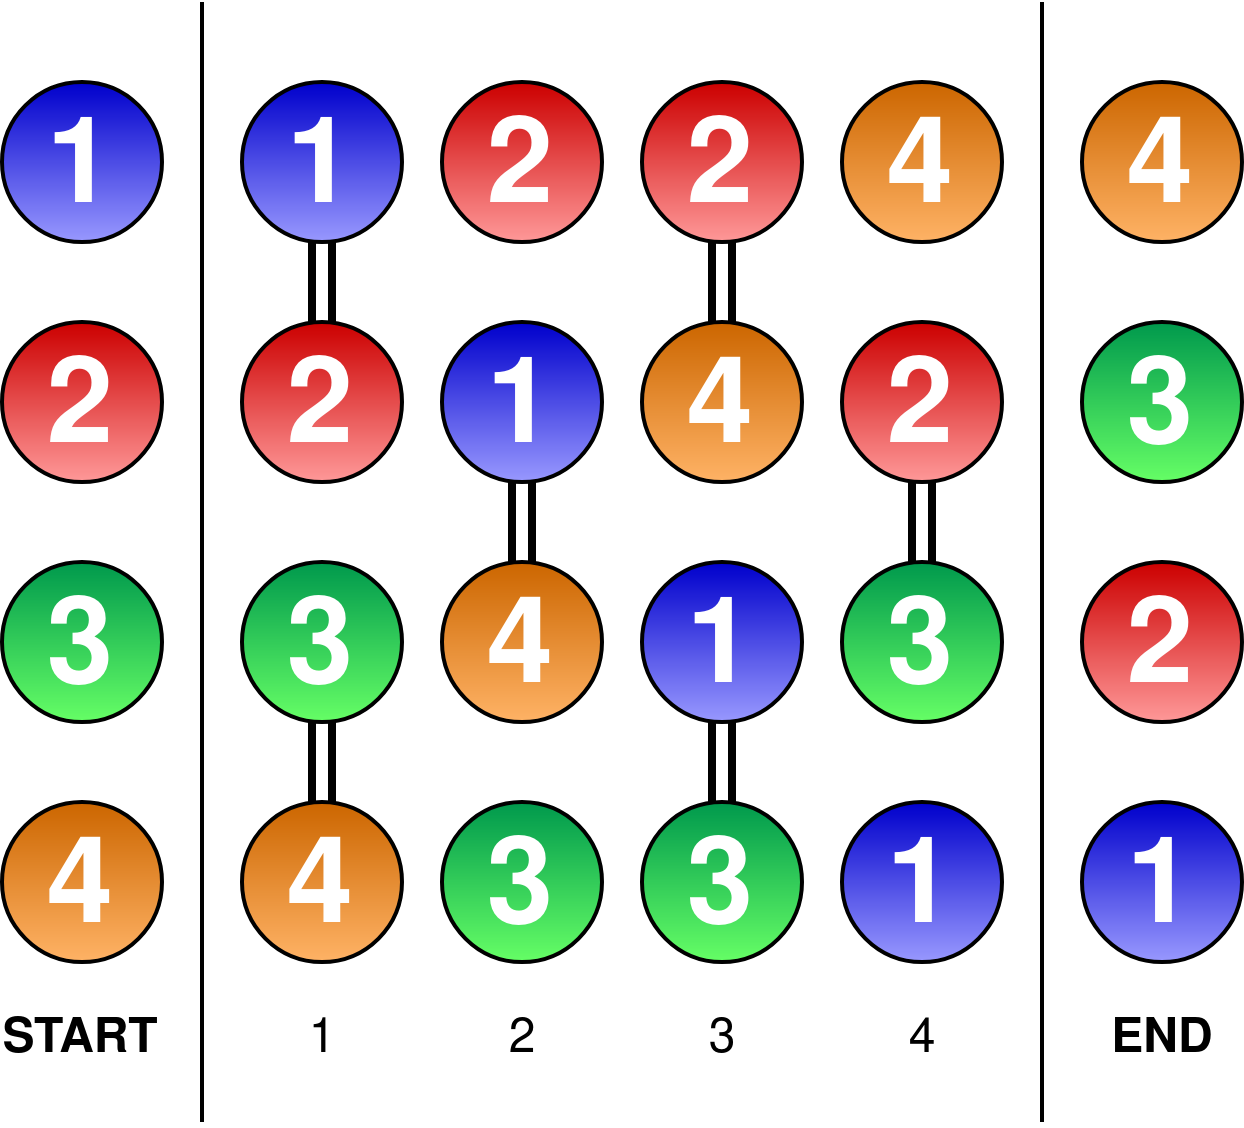
\includegraphics[width=0.45\textwidth]{swap.png}
 \caption{(Color online) Pictorial representation of the swap network used in our simulation in the case of $N=4$ neutrinos.}
\label{fig:swap_network}
\end{figure}

At the end of a sequence of $N$ such combined operations we will have implemented the full unitary in equation \eqref{eq:pair_prop_app} while, at the same, we inverted the ordering of qubits, as shown in Figure \ref{fig:swap_network}. This approach requires exactly the minimum number $\binom{N}{2}$ of nearest-neighbor pair operations, while the shifted ordering can be controlled completely, and efficiently, by classical means. Note that if we were to repeat at this point the same swap network in reverse order, the full unitary will correspond to a second order step for time $2t$ and the final ordering of qubits will be restored to its original one. This is the strategy used in Refs.~\cite{Roggero2021a,Roggero2021b} to study the neutrino Hamiltonian with Matrix Product States. In this first implementation on quantum hardware, we focus instead on a single, linear-order, time step.

Note that since we are only using nearest neighbor two-qubit gates, the total number of entangling gates required for a full time evolution step is bounded from above by $3\binom{N}{2}$ while the maximum number of single qubit operations is bounded by $15\binom{N}{2}$. As we will see in the results presented below, the presence of a large number of arbitrary single qubit rotations seems to be the limiting factor in implementing this scheme on the quantum device we used in this first exploration.

In order to study the build up of correlations and entanglement generated by the time-evolution under the Hamiltonian in (\ref{cno_hamiltonian}) we first initialize a system of $N=4$ qubits in the following product state 
\begin{equation}
\ket{\Phi_0} = \ket{e}\otimes\ket{e}\otimes\ket{x}\otimes\ket{x} = \ket{0011}
\end{equation}
We then preform one step of time evolution for time $t$ by applying the $N$ layers of nearest-neighbor gates as described in the previous section. This corresponds to a single Trotter-Suzuki step for different values of the time-step.
The four SU(2) spins representing the neutrinos are mapped to qubits $(2,1,3,4)$ on the IBMQ Vigo quantum processor~\cite{IBMQ_Vigo}, whose connectivity is schematically depicted in Figure \ref{fig:vigo}. The resulting qubits are linearly connected, allowing us to carry out natively the complete simulation scheme depicted in Figure \ref{fig:swap_network} above.

\begin{figure}[h]
    \centering
    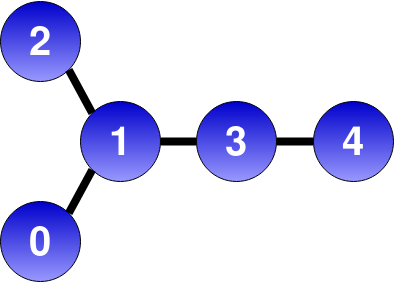
\includegraphics[width=0.25\textwidth]{vigo.png}
    \caption{(Color online) Layout of the IBM Quantum Canary Processor Vigo~\cite{IBMQ_Vigo}. Shown are the five qubits, labeled from 0 to 4, and their connectivity denoted as solid black lines.}
    \label{fig:vigo}
\end{figure}

The first observable we compute is the inversion probability $P_{\text{inv}}(t)$, the probability that a neutrino is measured to not be in its original flavor state, of each individual neutrino as a function of time. Note that under the simultaneous exchanges $1\leftrightarrow4$ and $2\leftrightarrow3$, while the Hamiltonian in (\ref{cno_hamiltonian} is invariant, the flavor content of the initial state $\ket{\Phi_0}$ gets reversed. Therefore, in the limit of no error, $P_{\text{inv}}(t)$ should be the same for the pairs of neutrinos $(1,4)$ and $(2,3)$. The errors in the approximation of the propagator (\ref{eq:pair_prop_app}) do not exactly follow this symmetry, with deviations in the range $3-7\%$. We show the results for $P_{\text{inv}}(t)$ obtained via the approximate evolution operator $U_2(t)$ as solid black lines in Figure \ref{fig:pop_03}, for the pair $(1,4)$, and in Figure \ref{fig:pop_12} for the pair $(2,3)$. The ideal, and symmetric, result is shown instead as a purple dashed line. We see that the approximation error is very small up to relatively large time $\eta t\approx 6$. As discussed earlier, this is in large part an effect of using the pair propagator $U_2(t)$ instead of the naive first order formula in equation \ref{eq:trotter1}. 

\begin{figure}[t]
 \centering
 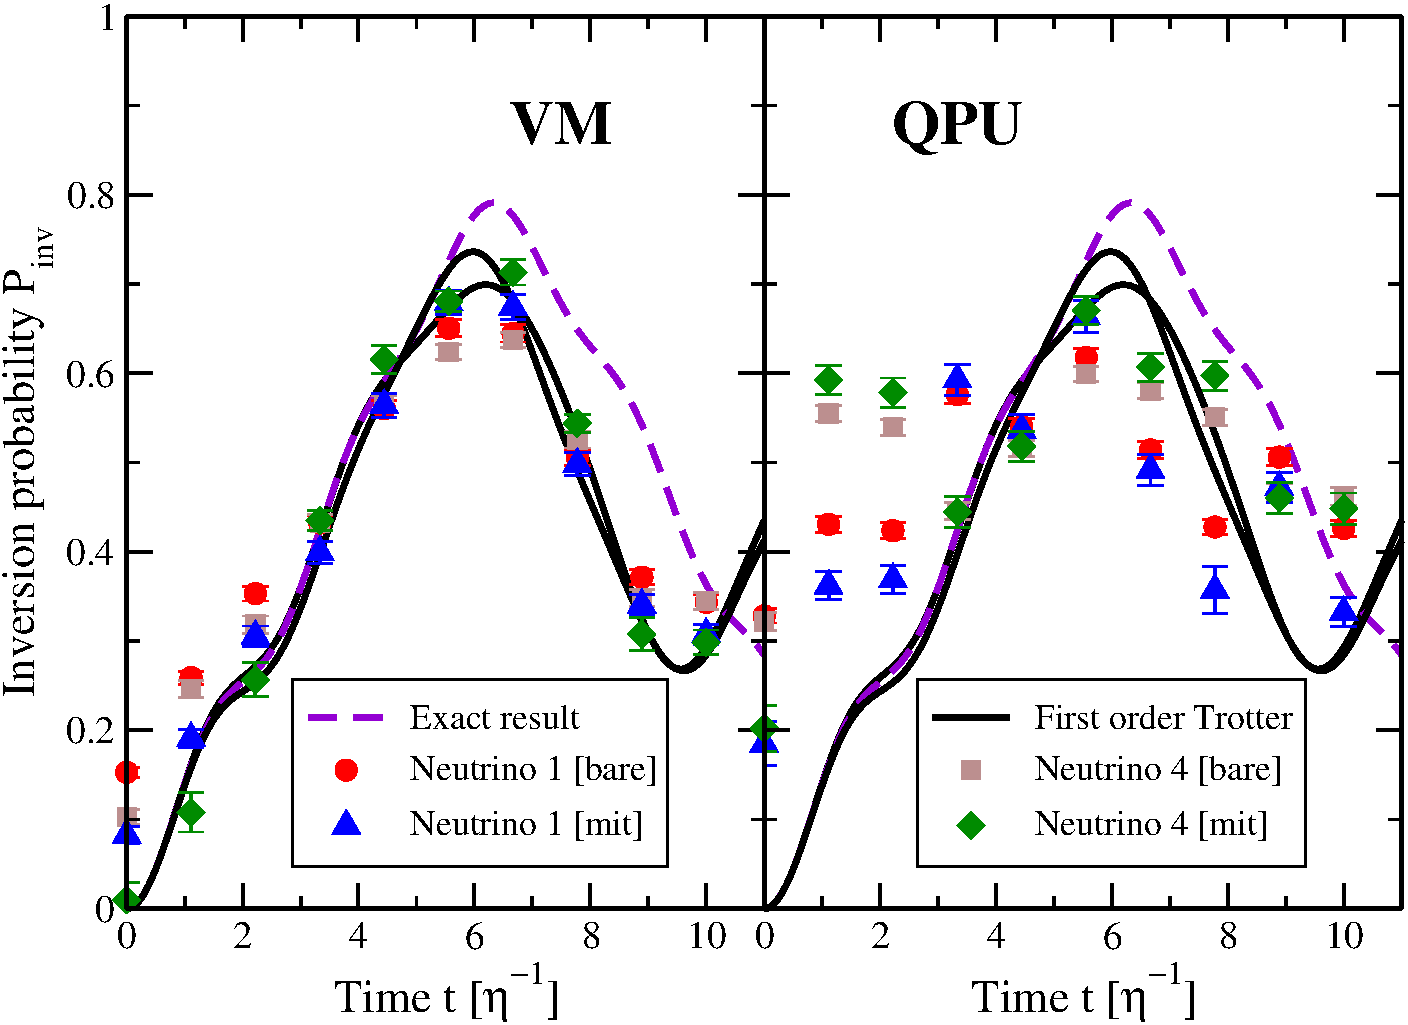
\includegraphics[width=0.49\textwidth]{pop_03.pdf}
 \caption{(Color online) Inversion probability $P_{inv(t)}$ for neutrinos one and four: the red circle and brown square correspond to the bare results, the blue triangle and the green diamond are obtained after error mitigation(see text). The left panel (VM) are virtual machine results while the right panel (QPU) are results obtained on the Vigo~\cite{IBMQ_Vigo} quantum device.}
\label{fig:pop_03}
\end{figure}

The results shown in Figure \ref{fig:pop_03} and Figure \ref{fig:pop_12} were obtained using either the real quantum device (right panels denoted QPU) or a local virtual machine simulation employing the noise model implemented in Qiskit~\cite{qiskit} (left panels denoted by VM) initialized with calibration data from the device. In both plots we report the results (denoted by [bare]) obtained directly from the simulation and including only statistical errors coming from a finite sample size (here and in the rest of the section we use $8192$ repetition, or ``shots", for every data point), as well as results obtained after performing error mitigation (denoted by [mit]). This corresponds to a final post-processing step that attempts to reduce the influence of the two main sources of errors: the read-out errors associated with the imperfect measurement apparatus and the gate error associated with the application of entangling gates. The latter error is dealt with using a zero noise extrapolation strategy (see~\cite{Endo2018,Dumitrescu2018} and section \ref{app:error_mit} for additional details). %The exact time dependence of $P_{\text{inv}}(t)$ is presented as the dashed line while the expected result for our first order Trotter approximation of the propagator in equation \eqref{eq:pair_prop_app} is presented as a continuous black line. 

\begin{figure}[t]
 \centering
 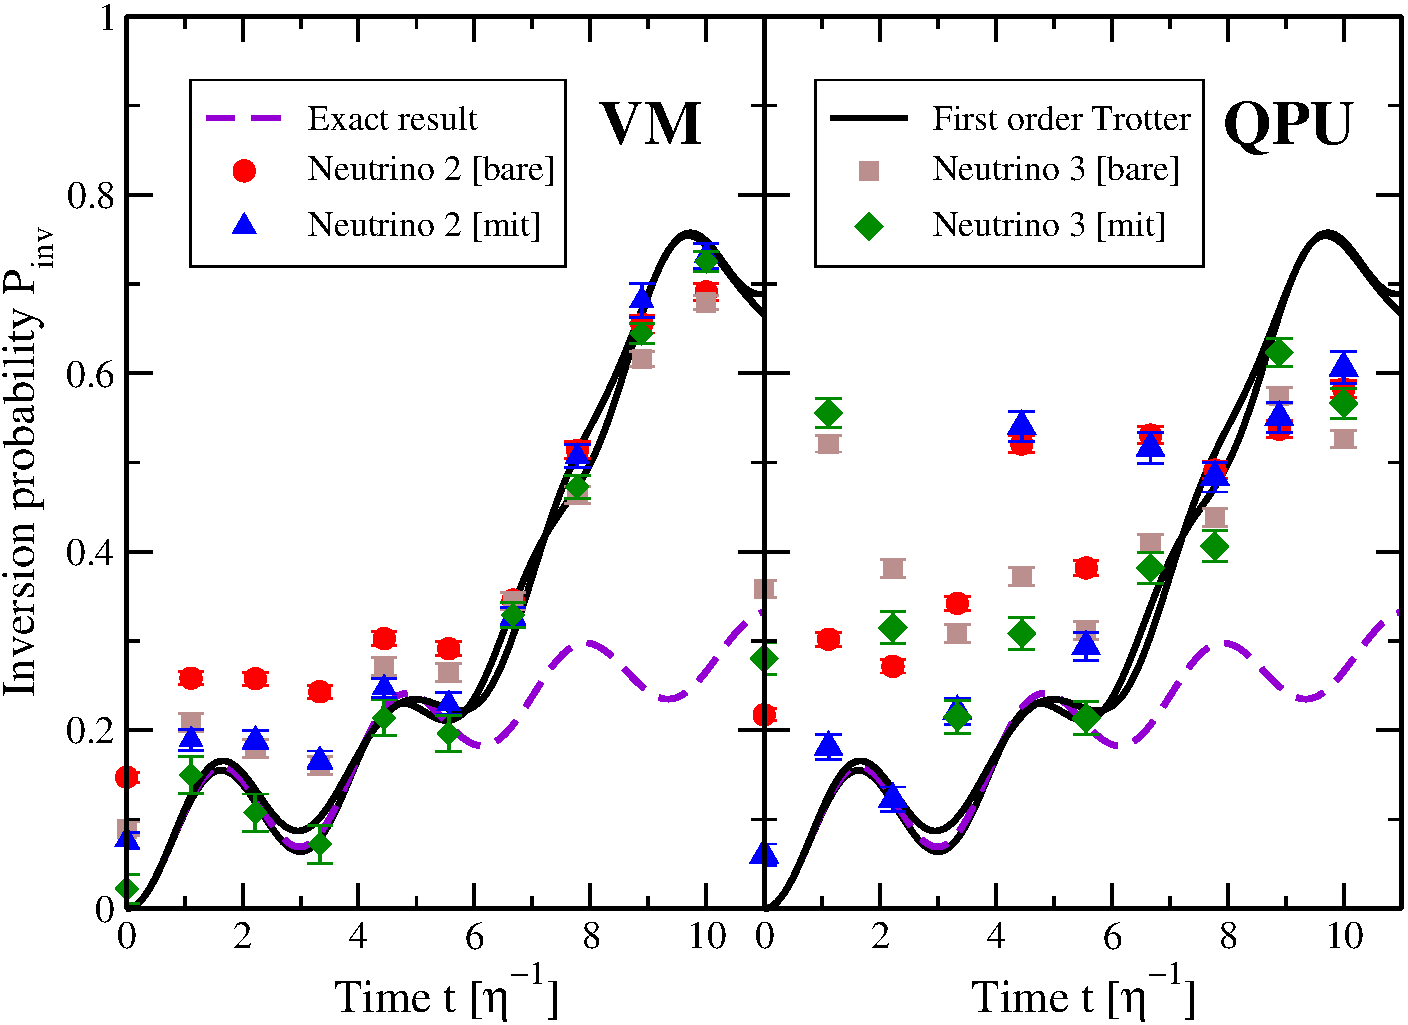
\includegraphics[width=0.49\textwidth]{pop_12.pdf}
 \caption{(Color online) Inversion probability $P_{\text{inv}}(t)$ for neutrinos twp and three. The notation is the same as for Figure \ref{fig:pop_03}.}
\label{fig:pop_12}
\end{figure}
 
As seen also in previous similar calculations (see for instance~\cite{roggero2020A,Roggero_nptodg}), the VM results obtained using the simulated noise are much closer to the ideal result than those obtained with the real device. This is also reflected in the fact that the error mitigation protocol is not as successful with the real QPU data as it is with the simulated VM data. This behaviour is possibly linked to the substantial noise caused by the presence of a large number of single qubit operations (up to 90 degree rotations for time evolution and two for state preparation) together with the relatively large CNOT count of 18. In fact, the performance of error mitigation for the results with the largest state preparation circuits presented in~\cite{Roggero_nptodg} is superior to the one obtained here, despite the use of the same device, the same error mitigation strategy and a comparable number of entangling gates (15 CNOT in that case) while the number of rotations was only 14. This suggests coherent errors constitute a considerable fraction of the overall error seen in the results above.

\begin{figure}[t]
 \centering
 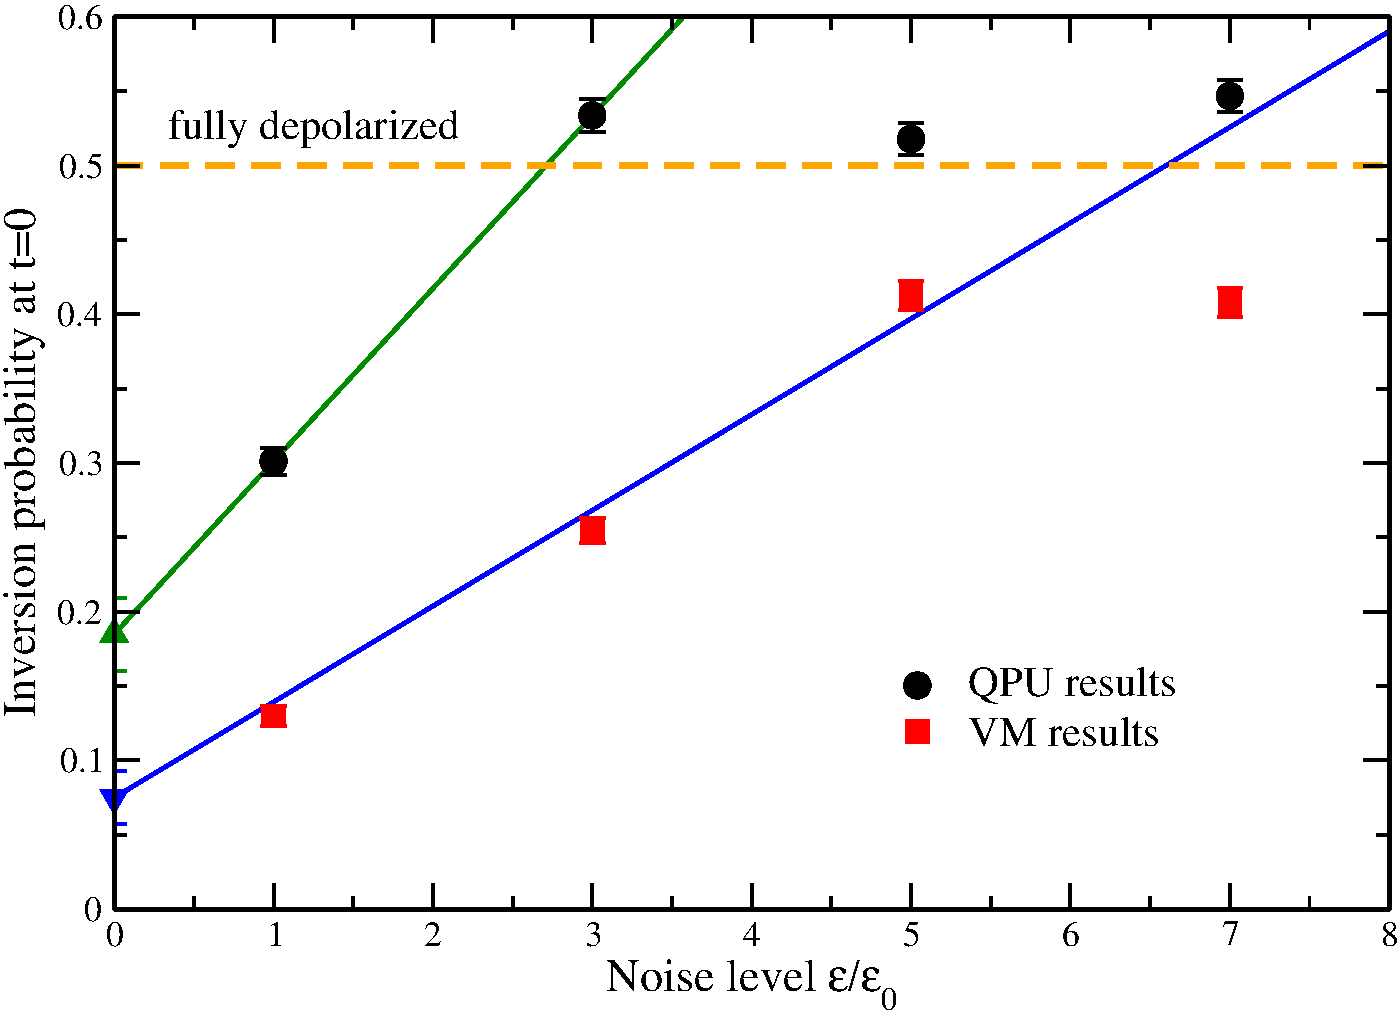
\includegraphics[width=0.49\textwidth]{extrap_at_t0.pdf}
 \caption{(Color online) Inversion probability $P_{\text{inv}}$ at the initial time $t=0$ for the first neutrino. Black solid circles are results from the Vigo QPU~\cite{IBMQ_Vigo} while the red squares correspond to results obtained using the VM with simulated noise. Also shown are extrapolations to the zero noise limit, for both the QPU (green line) and the VM (blue line), together with the extrapolated value (greed triangle up and blue triangle down respectively). The dashed orange line denotes the result for a maximally mixed state.}
\label{fig:pop_extrap}
\end{figure}

In order to highlight the difficulties encountered when performing noise extrapolation for this data, we plot in Figure \ref{fig:pop_extrap} the results obtained from both the QPU (black circles) and the VM (red squares) for the inversion probability of the first neutrino at the initial time $t=0$ together with a linear extrapolation using the first two points for the QPU (green line) and the first three points for the VM (blue line). The exact result is of course $P_{\text{inv}}(0)=0$ and we see that neither strategy is able to predict the correct value. The horizontal dashed line is the value expected when the system is in the maximally mixed state, corresponding to full depolarization. As shown in the data, for the real QPU results, only the first level of noise extrapolation contains useful information and a more gentle noise amplification strategy, like the one proposed in \cite{He2020}, could provide a substantial advantage over the strategy adopted here.

\section{Dynamics of entanglement}

In order to track the evolution of entanglement in the system we perform complete state tomography for each of the six possible qubit pairs in our system by estimating, for each pair $(k,q)$, the 16 expectation values
\begin{equation}
\label{eq:simple_mat_els}
M^{k,q}_{\alpha,\beta}(t) = \langle \Phi(t)\lvert P_k^\alpha\otimes P_q^\beta \rvert \Phi(t)\rangle\;,
\end{equation}
with $P^{\alpha}_k\in\{I,X,Y,Z\}$ being a Pauli matrix acting on the $k^\text{th}$ qubit and $\ket{\Phi(t)}$ the state obtained from $\ket{\Phi_0}$ by applying the time-evolution operator as in equation \eqref{eq:schroedinger-eq}. In principle, we might reconstruct the density matrix for the pair of qubits $(k,q)$ directly from these expectation values as
\begin{equation}
\label{eq:naive_dm}
{\rho}^D_{kq}(t) = \sum_{\alpha=1}^4\sum_{\beta=1}^4M^{k,q}_{\alpha,\beta}(t)P_k^\alpha\otimes P_q^\beta\;.
\end{equation}
In practice however, we can only estimate the matrix elements $M^{k,q}_{\alpha,\beta}(t)$ to some finite additive precision, and the approximation in equation \eqref{eq:naive_dm} is not guaranteed to be a physical density matrix (positive definite and with trace equal to 1). In this work we use the common approach (see eg.~\cite{Banaszek1999}) of performing a maximum-likelihood (ML) optimization, while enforcing the reconstructed density matrix ${\rho}^{ML}_{kq}(t)$ to be physical. We note in passing that it is possible to devise operator basis that are more robust than the choice used in equation \eqref{eq:simple_mat_els} (see eg.~\cite{Czartowski2020}) but we didn't explore this further in our work.

In order to propagate the effect of statistical errors into the final estimator for ${\rho}^{ML}_{kq}(t)$, we use a re-sampling strategy similar to what was introduced in~\cite{Roggero_nptodg} but using a Bayesian approach to determine the empirical posterior distribution. We provide a detailed description of the adopted protocol in subsection \ref{app:posterior_sampling}.

\subsection{Entanglement Entropies}

As we mentioned in the introduction, one of the main differences between a mean field description and the full many-body description of the dynamics of the neutrino cloud is the absence of quantum correlations, or entanglement, in the former. Past work on the subject~\cite{Cervia:2019,Rrapaj2020} looked at the single spin entanglement entropy defined as
\begin{equation}
 S_k(t) = - \text{Tr} \left[{\rho}_k(t)\log_2\left({\rho}_k(t)\right)\right]\;,
\end{equation}
with ${\rho}_k(t)$ the reduced density matrix of the $k$-th spin. A value of the entropy $S_k(t)$ different from zero indicates the presence of entanglement between the $k$-th neutrino and the rest of the system.

In our setup, we compute the one-body reduced density matrix from the maximum-likelihood estimator of the pair density matrix defined above, explicitly
\begin{equation}
S^{ML}_{k;q}(t) = - \text{Tr} \left[{\rho}^{ML}_{k;q}(t)\log_2\left({\rho}^{ML}_{k;q}(t)\right)\right]\;,
\end{equation}
where the reduced density matrices are computed from
\begin{equation}
{\rho}^{ML}_{k;q}(t) = \text{Tr}_q \left[{\rho}^{ML}_{kq}(t)\right]\;,
\end{equation}
and $\text{Tr}_q$ denotes the trace over the states of the $q$-th qubit.
We combine the three values obtained in this way for each neutrinos as follows: the estimator for the single-spin entanglement entropy is obtained from the average 
\begin{equation}
S^{\text{avg}}_k(t) = \frac{1}{3} \sum_{q}S^{ML}_{k;q}(t)\;,
\end{equation}
summing over pairs containing the k-th spin, while as an error estimate we use the average of the three errors.

\begin{figure}
 \centering
 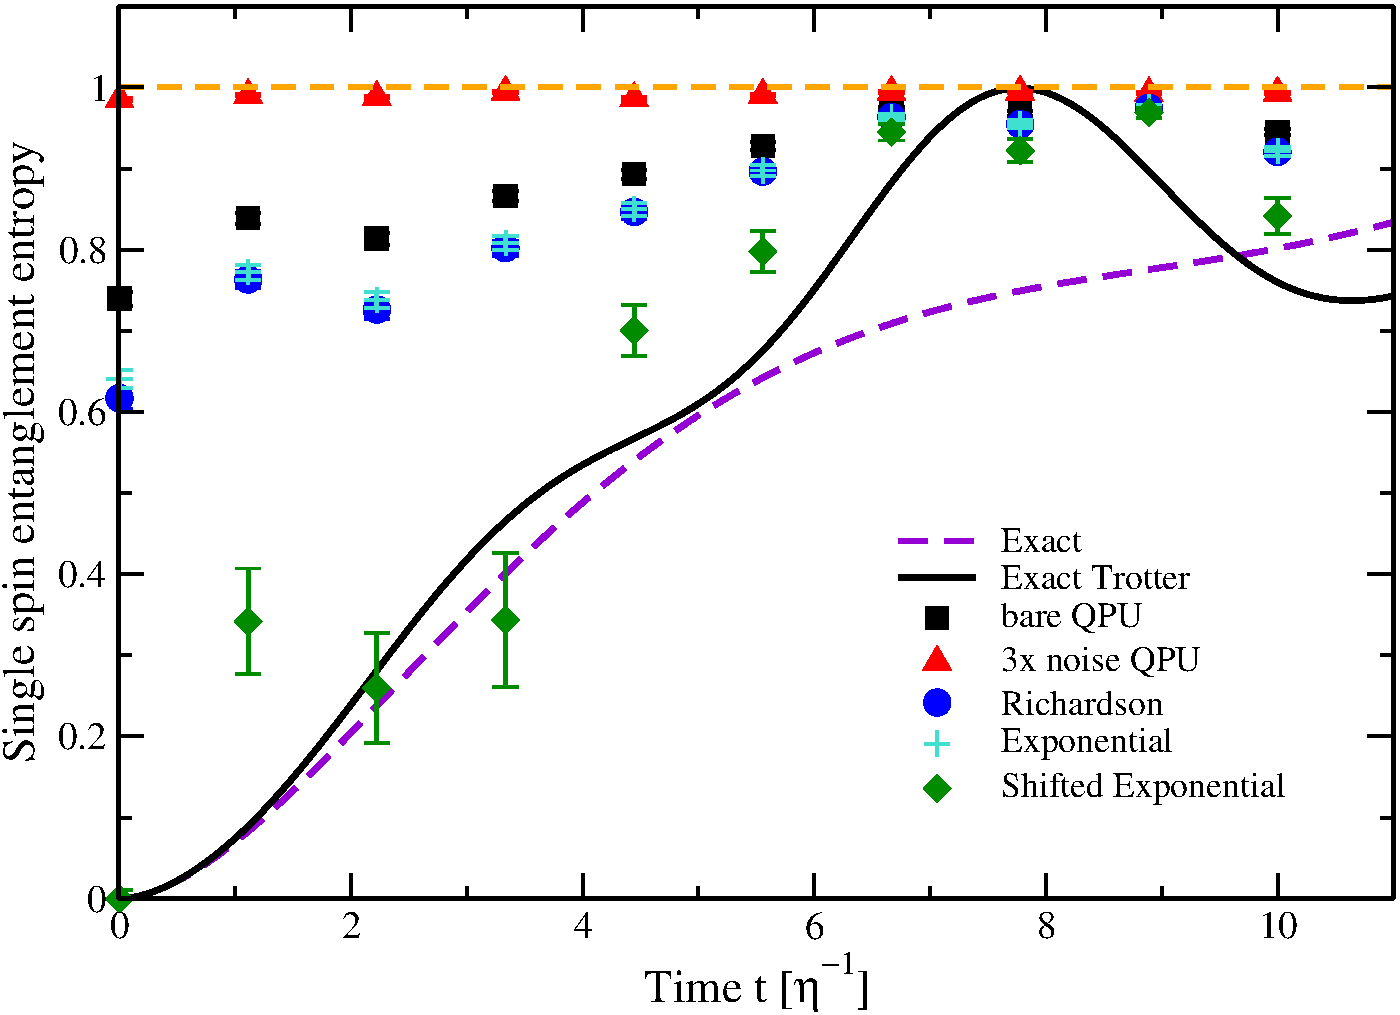
\includegraphics[width=0.49\textwidth]{sq1_ent.pdf}
 \caption{(Color online) Single spin entanglement entropy for neutrino 2. Black square are bare results obtained from the QPU, red triangles are results obtained by amplifying the noise to $\epsilon/\epsilon_0=3$, the blue circles are obtained using Richardson extrapolation, the turquoise plus symbols indicate results obtained using the standard exponential extrapolation and the green diamonds correspond to the results obtained from a shifted exponential extrapolation using the maximum value of the entropy (indicated as a dashed orange line).}
\label{fig:sq_ent1}
\end{figure}

As for the case of the inversion probability $P_{\text{inv}}(t)$ studied in the previous section, the substantial noise present in the QPU data prevents us from using the full set of results at the four effective noise levels. In order to overcome this difficulty, we have performed zero noise extrapolations using only results for effective noise levels $r=\epsilon/\epsilon_0=(1,3)$ and performed a Richardson extrapolation (in this case equivalent to a simple linear fit as done in \cite{Dumitrescu2018}), a two point exponential extrapolation~\cite{Endo2018}, and an exponential extrapolation with shifted data. The latter technique consists in shifting the data for the entropy by $-1$ (its maximum value) so that the result, in the limit of large noise, tends to 0 instead of $\log_2(2)=1$. We then shift back the result obtained after extrapolation. The exponential extrapolation method is well suited for situations where expectation values decay to zero as a function of the noise strength $\epsilon$, while maintaining a consistent sign, and this shift allows us to make the data conform to this ideal situation (section \ref{app:error_mit} for more details on the method). The impact on the efficacy of the error mitigation is dramatic as can be seen in the results presented in Figure \ref{fig:sq_ent1} for the entropy of the second neutrino (the entropies for the other neutrinos follow a similar pattern; see subsection \ref{app:sq_ent} for all four results). The results with the standard exponential extrapolation are presented as the turquoise plus symbols, they are almost the same as those obtained using Richardson extrapolation (blue circles) and show a significant systematic error. On the contrary, the results obtained with the Shifted Exponential extrapolation (green diamonds) are much more close to the expected results with our pair propagator (solid black curve). We expect more general multi-exponential extrapolation schemes, like those proposed in Refs.~\cite{giurgicatiron2020,cai2020}, to enjoy a similar efficiency boost in the large noise limit achieved with deep circuits.

\begin{figure}
 \centering
 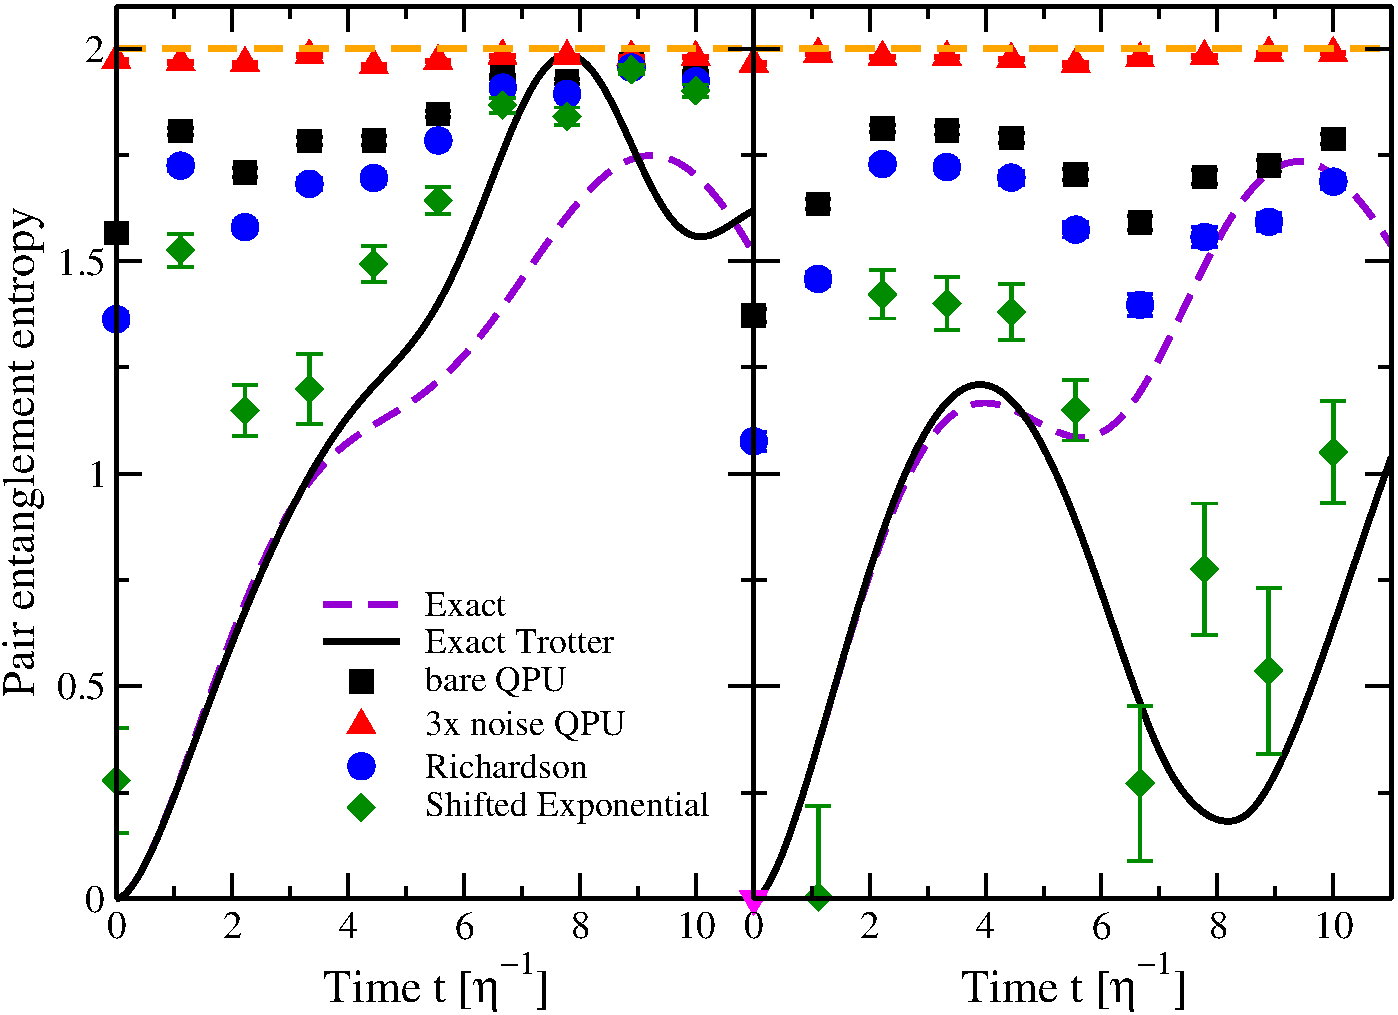
\includegraphics[width=0.49\textwidth]{pairs04_ent.pdf}
 \caption{(Color online) Pair entanglement entropy for the neutrino pair $(1,2)$ starting as $\ket{e}\otimes\ket{e}$ (left panel) and pair $(2,4)$ which starts as the flavor state $\ket{e}\otimes\ket{x}$ (right panel). Results obtained directly from the QPU are shown as black squares ($r=1$) and red triangles ($r=3$) while blue circles and green diamonds indicate mitigated results using Richardson and the Shifted Exponential extrapolations respectively. For the Shifted Exponential ansatz we use the maximum value of the entropy (indicated as a dashed orange line).The magenta triangle indicates a mitigated result with Shifted Exponential extrapolation below zero within errorbars.}
\label{fig:pair_ent_04}
\end{figure}

Using the reconstructed pair density matrix ${\rho}^{ML}_{kq}(t)$, we can clearly also evaluate directly the entanglement entropy of the pair
\begin{equation}
 S^{ML}_{kq}(t) = - \text{Tr} \left[{\rho}^{ML}_{kq}(t)\log_2\left({\rho}^{ML}_{kq}(t)\right)\right]\;.
\end{equation}
In Figure \ref{fig:pair_ent_04} we show the result of this calculation for the pair $(1,2)$, which started as electron flavor at $t=0$, and the pair $(2,4)$ which started instead as heavy flavor states.

\subsection{Concurrence}

In order to better understand these quantum correlations, we also compute the concurrence~\cite{Wooters1998} for all the pair states. This measure of entanglement is defined for a two-qubit density matrix as
\begin{equation}
\label{eq:concurr}
C(\rho) = \max\left\{0,\lambda_0-\lambda_1-\lambda_2-\lambda_3\right\}\;,
\end{equation}
where $\lambda_i$ are the square roots of the eigenvalues, in decreasing order, of the non-Hermitian matrix
\begin{equation}
M = \rho\left(Y\otimes Y\right)\rho^*\left(Y\otimes Y\right)\;,
\label{eq:concurr_M}
\end{equation}
with the star symbol indicating complex conjugation. The usefulness of this measure is its relation with the entanglement of formation~\cite{Hill1997,Wooters1998}, which is the minimum number of maximally-entangled pairs needed to represent $\rho$ with an ensemble of pure states~\cite{Hill1997}. 

The definition of concurrence in equation \eqref{eq:concurr} does not lend itself as easily to be adapted in an error extrapolation procedure as the one we used to obtain the mitigated results in the previous sections. This is due to the presence of the max function in the definition of the concurrence: when the error is sufficiently strong to make the difference in eigenvalues
\begin{equation}
\widetilde{C}(\rho) = \lambda_0-\lambda_1-\lambda_2-\lambda_3
\end{equation}
negative, the concurrence in equation \eqref{eq:concurr} ceases to carry information about the error free result. For this reason, we will regard $\widetilde{C}$ as an ``extended concurrence" which varies smoothly for large error levels and perform the truncation to positive values only after the zero noise extrapolation.
The results obtained from the simulation on the Vigo QPU are shown in Figure \ref{fig:conc_pair_04} for two pairs of neutrinos: pair $(1,2)$ starting as like spin at $t=0$ and pair $(2,4)$ which started as opposite flavors. The complete set of results for all pairs can be found in Figure \ref{fig:sq_all} in subsection \ref{app:sq_ent}.


\begin{figure}[tbh]
 \centering
 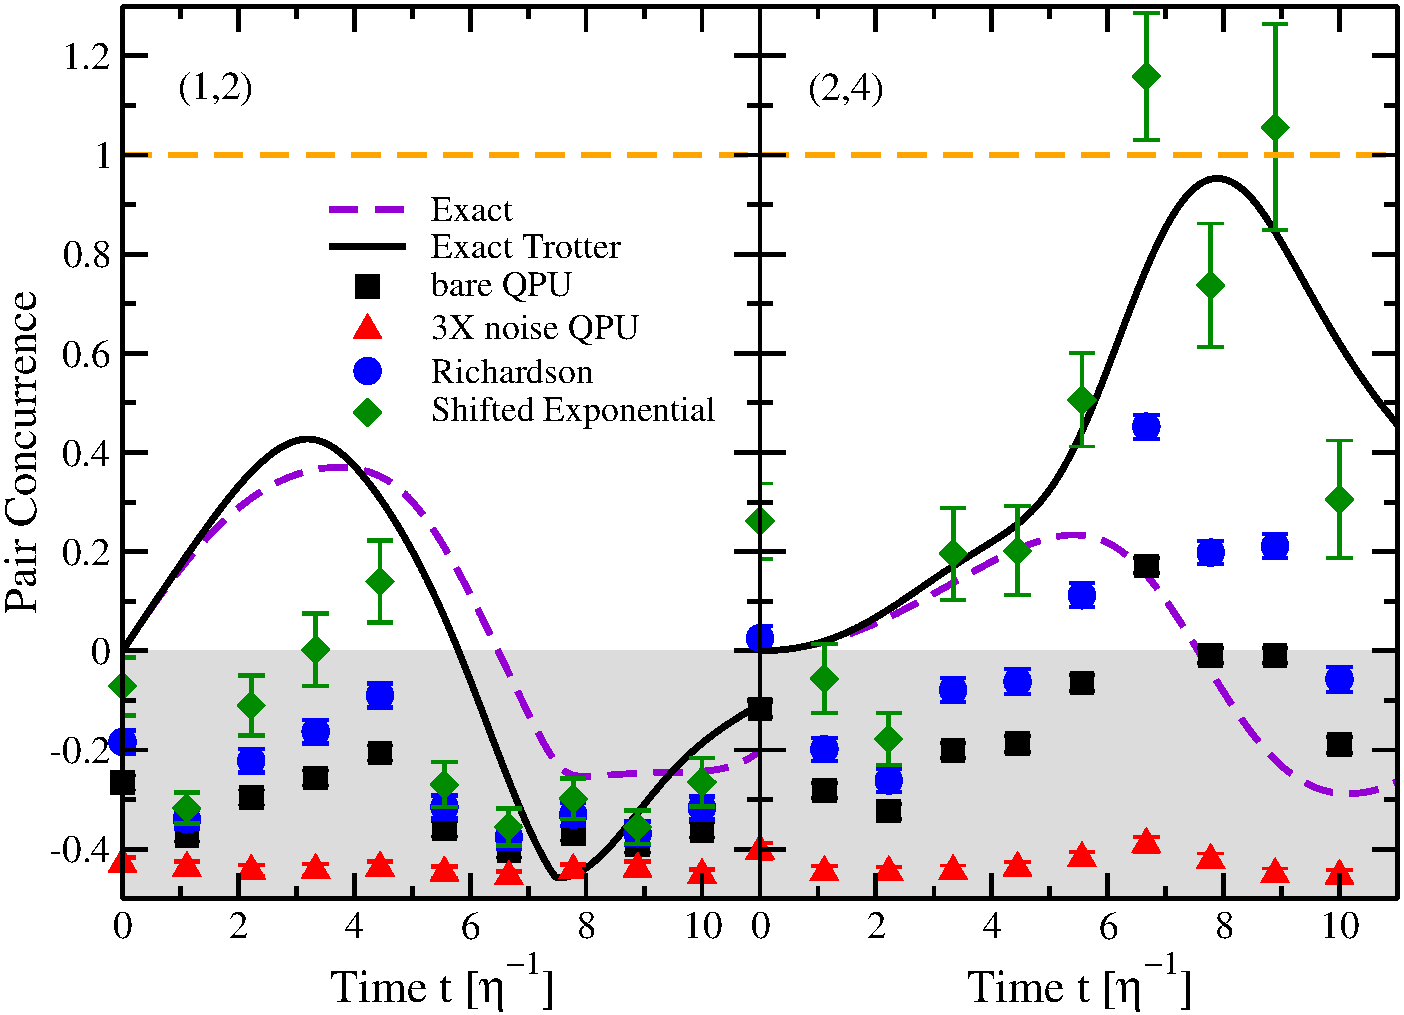
\includegraphics[width=0.49\textwidth]{conc_pair04.pdf}
 \caption{(Color online) Extended concurrence $\widetilde{C}$ for two pairs of neutrinos, $(1,2)$ in the left and $(2,4)$ in the right panel. The convention for the curves and date point used here is the same as in Figure \ref{fig:pair_ent_04}. The gray area indicates the region where the concurrence $C(\rho)$ is zero. The maximum value for the concurrence is shown as a dashed orange line.}
\label{fig:conc_pair_04}
\end{figure}


The bare results are shown as black squares and we can immediately notice why the definition of $\widetilde{C}$ is so important in our case: the only bare data point with a measurable concurrence $C(\rho)$ is at $t\approx6.7\eta^{-1}$ for pair $(2,4)$ (the right panel in Figure \ref{fig:conc_pair_04}) while all the other results, including those obtained with a larger noise level (red triangles), are compatible with zero. In this situation, no mitigation of $C(\rho)$ would be possible.

By keeping the negative contributions, we see that the bare results often contain a substantial signal, while those at a higher error rate are already almost at the asymptotic value $\widetilde{C}=-0.5$ expected for a completely depolarized system. Note that our results seem to converge to a larger asymptotic value of $\widetilde{C}\approx-0.44$ instead of $\widetilde{C}=-0.5$. We can empirically explain this difference as the effect of statistical fluctuations. This allowed us to perform error extrapolation using both the Richardson and Shifted Exponential ansatz. Similarly to what we observed for the entanglement entropies in the previous section, the Shifted Exponential ansatz (with shift $-0.5$) produces consistently better results than Richardson extrapolation. This indicates that we are more close to the asymptotic large error regime than the small error limit used to motivate a polynomial expansion. The resilience of the exponential extrapolations to large errors, especially augmented by an appropriate shift, is seen here to be critical in extracting physical information from quantum simulations carried out near the coherence limit of the device used for the implementation.    

% \begin{acknowledgments}
% This work was supported by the InQubator for Quantum Simulation under U.S. DOE grant No. DE-SC0020970, by the Quantum Science Center (QSC), a National Quantum Information Science Research Center of the U.S. Department of Energy (DOE), by the U.S. Department of Energy under grant No. DE-FG02-00ER41132, DE-SC0021152 and by the U.S. National Science Foundation under Grants No. PHY-1404159 and PHY-2013047. 
% Benjamin Hall acknowledges support from the U.S. Department of Energy (DOE) through a quantum computing program sponsored by the Los Alamos National Laboratory (LANL) Information Science \& Technology Institute.
% We  acknowledge  use  of the  IBM  Q  for  this  work. The  views  expressed  are those of the authors and do not reflect the official policy or position of IBM or the IBM Q team. 
% \end{acknowledgments}

\section{Error mitigation}
\label{app:error_mit}
In the following subsections we describe in more detail the error mitigation techniques used in this work. 

\subsection{Propagation of statistical uncertainties}
\label{app:posterior_sampling}

In this section we describe the procedure we have adopted for propagating statistical errors in the results reported previously. We found that careful treatment of statistical errors was important for non linear functions of the expectation values like entropy and concurrence of a reconstructed density matrix.

In the following, we will symbolically denote as $\langle O\rangle$, expectation values of Pauli operators which can be measured directly on the device. These are, for instance, the expectation values $\langle X X\rangle$, $\langle X Y\rangle$, etc. needed to reconstruct a two-qubit density matrix.

We use a Bayesian approach to perform inference from the bare counts obtained from the device. The idea is best described initially for the simple case of a single qubit measurement. The probability of obtaining $m$ measurements of the state $\ket{1}$ out of a total of $M$ trials can be modelled as a binomial distribution
\begin{equation}
P_b(m;p) =     \binom{M}{m}p^{m}(1-p)^{M-m}\;,
\end{equation}
with $p$ the probability of a $\ket{1}$ measurement. In order to infer the parameter $p$ from a given sample $m_i$ of measurement outcomes, we use Bayes' theorem
\begin{equation}
P(p|m_i) = \frac{P(m_i|p)P(p)}{\int dq P(m_i|q)P(q)}\;.
\end{equation}
For the single qubit measurement, we use the binomial distribution as likelihood $P(m_i|p)$ and, in order to obtain a posterior $P(p|m_i)$ in closed form, we use the conjugate prior of the binomial: the beta distribution
\begin{equation}
P_\beta(p;\alpha,\beta) = \frac{\Gamma(\alpha+\beta)}{\Gamma(\alpha)\Gamma(\beta)} p^{\alpha-1}(1-p)^{\beta-1}\;.
\end{equation}
Here $\alpha,\beta>0$ are the parameters defining the distribution and with $\alpha=\beta=1$ we obtain a uniform distribution. The advantage of using the Beta distribution as a prior is that, after a measurement $m_i$ of the system is available, the parameters $(\alpha_0,\beta_0)$ of the prior distribution get updated as
\begin{equation}
\alpha_i = \alpha_0 + m_i\quad\beta_i=\beta_0 + M-m_i\;.
\end{equation}
Intuitively we can interpret the parameters $(\alpha_0,\beta_0)$ of the prior as assigning an a-priori number of measurements to the measurement outcomes, which are then updated as more measurements are performed. In this work we used a simple uniform prior corresponding to the choice $\alpha_0=\beta_0=1$ for the prior parameters.

After the inference step described above, we calculate the expectation value of a generic non-linear function $\langle F[O]\rangle$ by sampling new outcomes $m'_k$ using the posterior distribution. More in detail, we generate a new artificial measurement $m'_k$ after the measured $m_i$ by the following procedure
\begin{itemize}
    \item sample a value $p'_k$ from the posterior $P(p'_k\lvert m_i)$ 
	\item sample a new measurement outcome $m_k'$ from the likelihood $P_b(m_k^\prime;p'_k)$
\end{itemize}

The new measurements $m_k'$ obtained in this way are then samples from the predictive posterior distribution.

Using an ensemble of size $L$ obtained in this way, we compute $\langle F[O]\rangle$ by taking an average of the results obtained for each individual sample
\begin{equation}
\langle F[O]\rangle \approx \frac{1}{L} \sum_{k=1}^L F[O_k]\;.
\end{equation}
The error bars reported previously are $68\%$ confidence intervals which we found in most cases where well approximated by a Gaussian approximation.

This scheme is complete only for single qubit measurements but a generalization to generic multi-qubit observables can be obtained in a straightforward way. In the situation where we are estimating expectation values over $N$ qubits, the probability of measuring  a specific collection of $N$ bit strings $m_i$ in $M$ repeated trials can be described with a multinomial distribution with $N$ probabilities. We use this distribution as the likelihood $P(m_i|\vec{p})$ in Bayes theorem and, for similar reasons as above, we take its conjugate prior distribution: the Dirichlet distribution (also initialized as uniform as for the Beta above). The procedure we follow is otherwise exactly equivalent to what we described above.

\subsection{Read-out mitigation}
The qubit measurements on a real device are not perfect and it is therefore important to understand the associated systematic errors. We refer the reader to Appendix.~H.1 of \cite{Roggero_nptodg} for a more detailed derivation of the exact procedure we employ and the motivations behind it. Here, we instead describe the main difference with the scheme described there which comes from the use of the Bayesian inference scheme described in the previous subsection.

In the calculations presented here, we work under the assumption that read-out errors are independent on each qubit and perform a set of $2N$ calibration measurements $c_i$ (requiring two separate executions) to extract the parameters $(\vec{e}_0,\vec{e}_1)$ of the noise model (see Eq.(H1) of \cite{Roggero_nptodg}). In order to consistently propagate the statistical uncertainties associated from the finite sample statistic used to estimate the noise parameters, we use an additional layer of Bayesian sampling using a binomial prior for the two error probabilities $(e^n_0,e^n_1)$ associated to each qubit $n$. 

Using a single pair of error probability vectors $\epsilon_i=(\vec{e}_0,\vec{e}_1)_i$, obtained either by direct measurement or by sampling from the posterior, we can generate a linear transformation $\mathbf{C}_i$ that maps a set of (in general multi-qubit) measurements $m_i$ to a new set $\widetilde{m}_i$ with reduced read-out errors (see \cite{Roggero_nptodg} for more details).

The complete procedure that we use to generate an ensemble of measurements $\{\widetilde{m}'_i\}$ with read-out mitigation starting from a single calibration measurement $c_i$ and Pauli operator measurement $m_i$ is as follows
\begin{itemize}
    \item sample a value $p'_k$ from the posterior $P(p'_k\lvert m_i)$ 
	\item sample a new measurement outcome $m_k'$ from the likelihood $P_b(m_i^\prime;p'_k)$
	\item for each qubit $n=\{1,\dots,N\}$
	\begin{itemize}
	    \item sample a pair $(e^{\prime n}_0,e^{\prime n}_1)$ of error probabilities from the posterior $P(e^n_0,e^n_1|c_i)$ 
	\end{itemize}
	\item use the sampled error probabilities $(\vec{e}'_0,\vec{e}'_1)$ to generate the linear transformation $\mathbf{C}'_k$ 
	\item apply the sampled correction matrix $\mathbf{C}'_l$ to $m_k'$ to obtain the read-out mitigated estimator $\widetilde{m}'_k$
\end{itemize}

The resulting ensemble of measurements can be used directly to estimate expectation values and confidence intervals as described above. In this way, we avoid having to explicitly construct the variance of the correction matrix $\mathbf{C}'_l$ using maximum likelihood estimation and then propagating the error perturbatively to arbitrary observables as done in \cite{Roggero_nptodg}.

\subsection{Zero-noise-extrapolation}
For observables like the inversion probability, we adopt the procedure developed in \cite{Roggero_nptodg}. For entanglement observables we adopt a two point shifted exponential extrapolation that we briefly describe here. We denote the entanglement observable as $\langle F[O]\rangle^{(L)}(r)$ where $L$ is the number of samples used and $r$ denotes the noise level of the circuit, proportional to the number of CNOT gates in the circuit. We first note that in the case of very high noise levels, denoted here with $\langle F[O]\rangle(r\rightarrow\infty)$ the density matrix corresponds to the maximally mixed state given by $\mathbbm{1}/4$. Therefore, the concurrence in this case is $-1/2$ and the pair entanglement saturates to $2$.

Using an estimate for the large noise expected value $\langle F[O]\rangle(r\rightarrow\infty)$, we can then consider a simple exponential extrapolation of the form
\begin{equation}
\langle F[O]\rangle^{(L)}(r)-\langle F[O]\rangle(r\rightarrow\infty) = A^{(L)}_F e^{-\alpha r}\, ,
\label{eq:exp-reshifted}
\end{equation}
with $\alpha $ and $A^{(L)}_F$ the parameters of the model which can be obtain using results at two different noise levels $r$ and $r^\prime$.
The zero-noise extrapolated result in this model corresponds to the limit $r\to0$ and is given simply by the estimated $A^{(L)}_F$. More explicitly this becomes
\begin{eqnarray}
A^{(L)}_F=\langle F[O]\rangle^{(L)}(r)\left(\frac{\langle F[O]\rangle^{(L)}(r^\prime)}{\langle F[O]\rangle^{(L)}(r)}\right)^{r/(r-r^\prime)}\, ,
\end{eqnarray}
and the zero noise extrapolated observable is
\begin{eqnarray}
\langle F[O]\rangle^{(L)}(0)=A^{(L)}_F+ \langle F[O]\rangle(r\rightarrow\infty)\, .
\end{eqnarray}
Finally, the estimated statistical error is obtained by calculating the standard deviation of the $L$ copies as above. 

\section{Additional data for concurrence and entanglement entropy}
\label{app:sq_ent}
Here we show the full set of results for both entanglement entropy and concurrence for all the other pairs of qubits not shown earlier. We denote with a magenta triangle, data-points that fall below zero for the entropy as in Figure \ref{fig:conc_pair_04}.

\begin{figure}[h!]
 \centering
 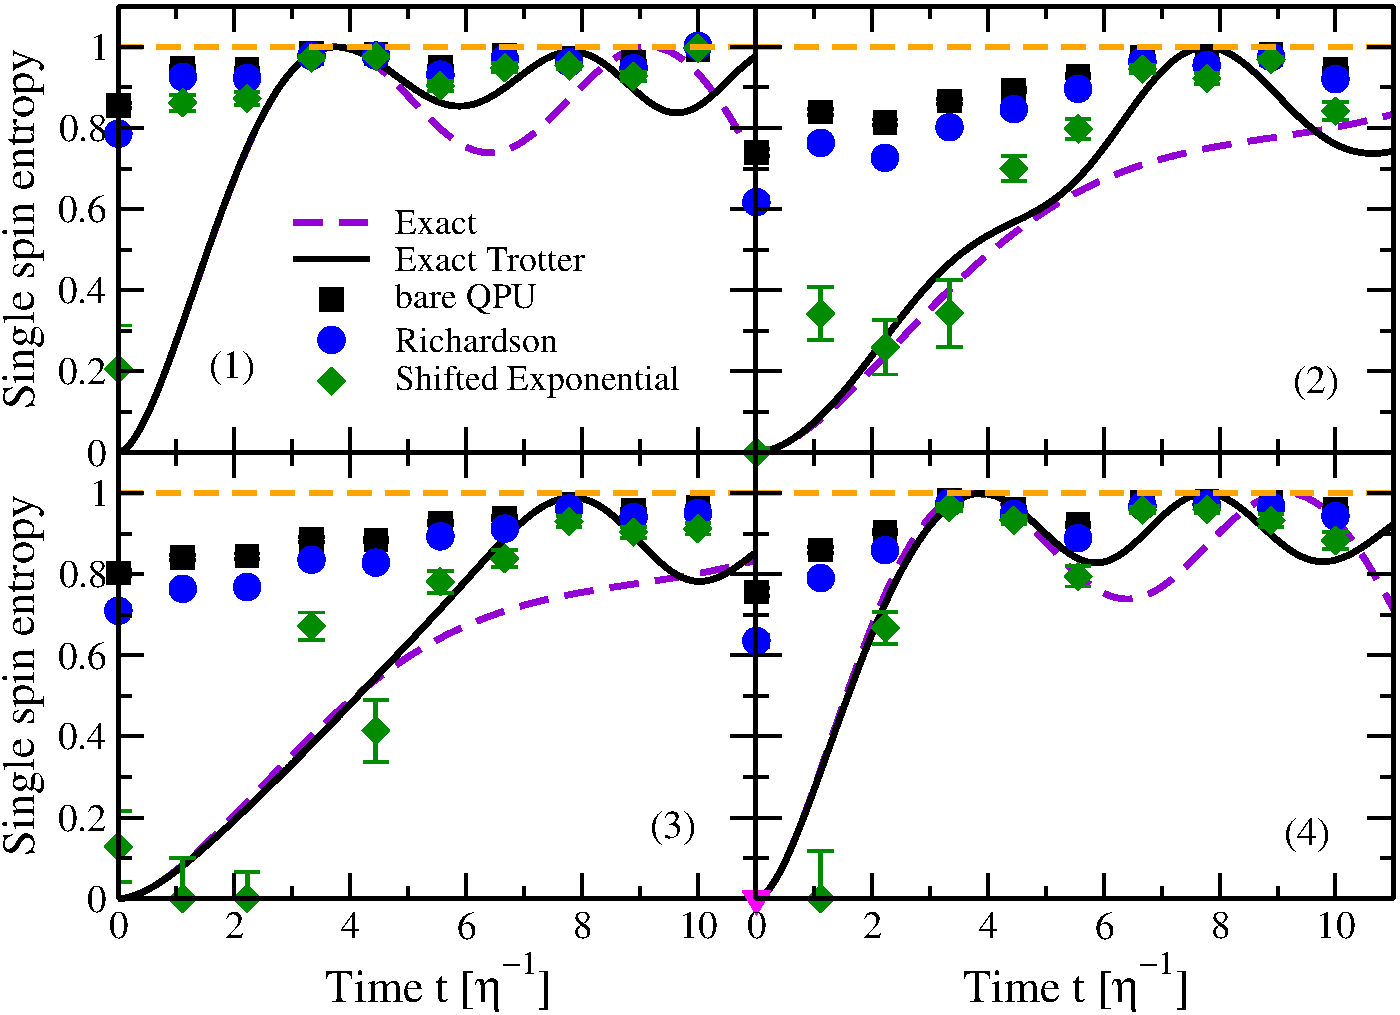
\includegraphics[width=0.49\textwidth]{sq_ent_all.pdf}
 \caption{(Color online) Single spin entanglement entropy for all four neutrinos. Black square are bare results obtained from the QPU, the blue circles are obtained using Richardson extrapolation and the green diamonds correspond to the results obtained from a shifted exponential extrapolation using the maximum value of the entropy (dashed orange line). The magenta triangle indicates a mitigated result with Shifted Exponential extrapolation below zero within errorbars.}
\label{fig:sq_all}
\end{figure}

\begin{figure}[H]
 \centering
 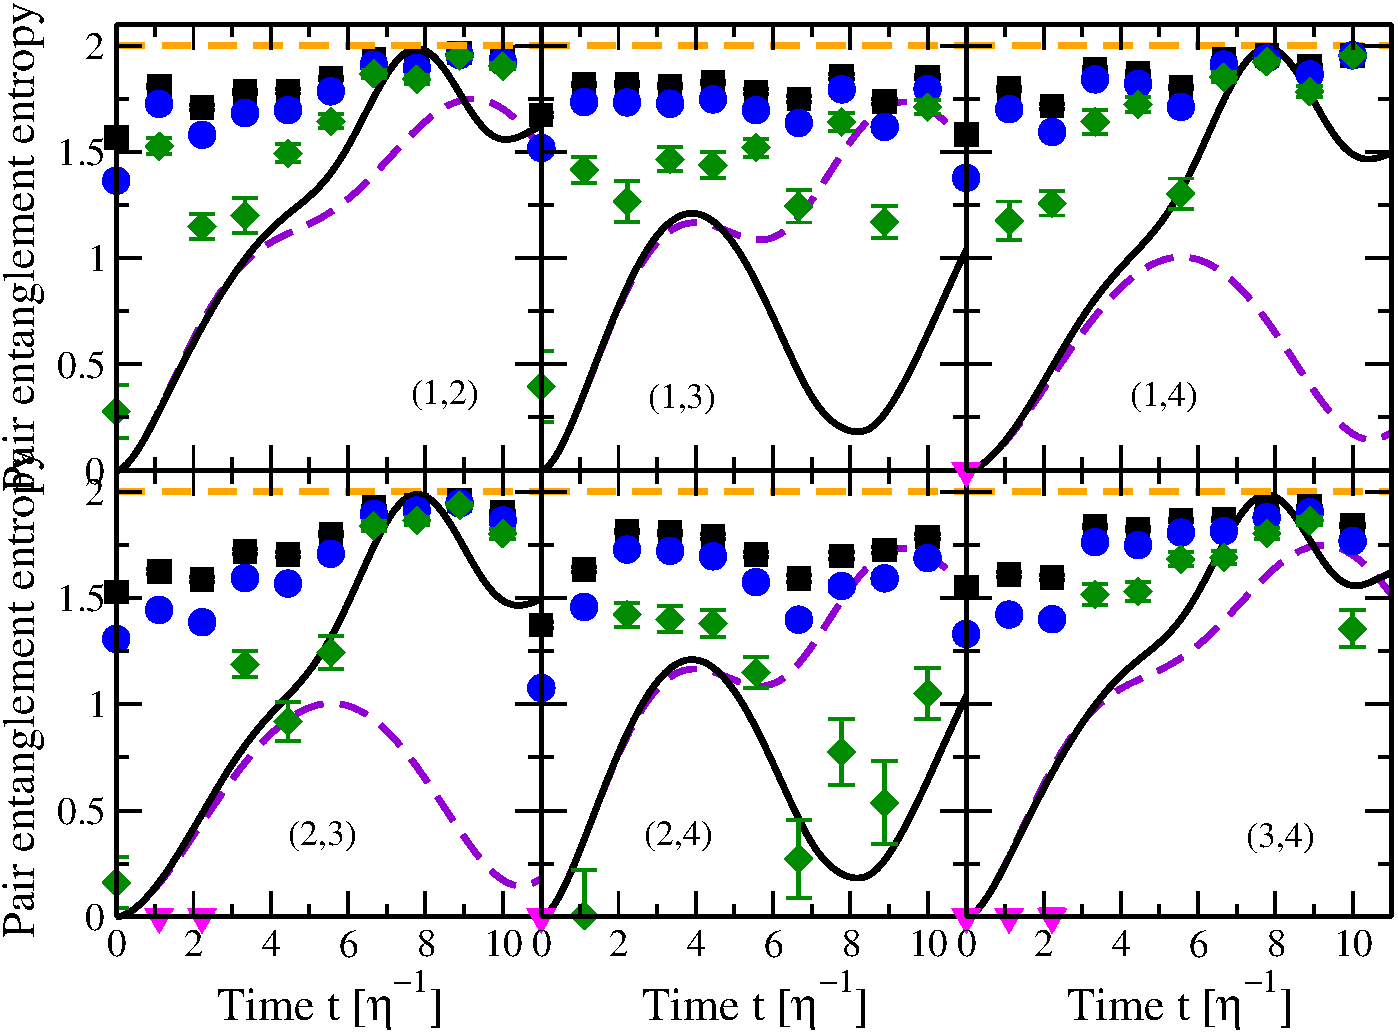
\includegraphics[width=0.49\textwidth]{all_pairs_ent.pdf}
 \caption{(Color online) Pair entanglement entropy for all pair of neutrinos. Black square are bare results obtained from the QPU, red triangles are results obtained by amplifying the noise to $\epsilon/\epsilon_0=3$, the blue circles are obtained using Richardson extrapolation and the green diamonds correspond to the results obtained from a shifted exponential extrapolation using the maximum value of the entropy (indicated as a dashed orange line). The magenta triangle points are mitigated results with Shifted Exponential extrapolation below zero within errorbars.}
\label{fig:pair_ent_all}
\end{figure}

\begin{figure}[H]
 \centering
 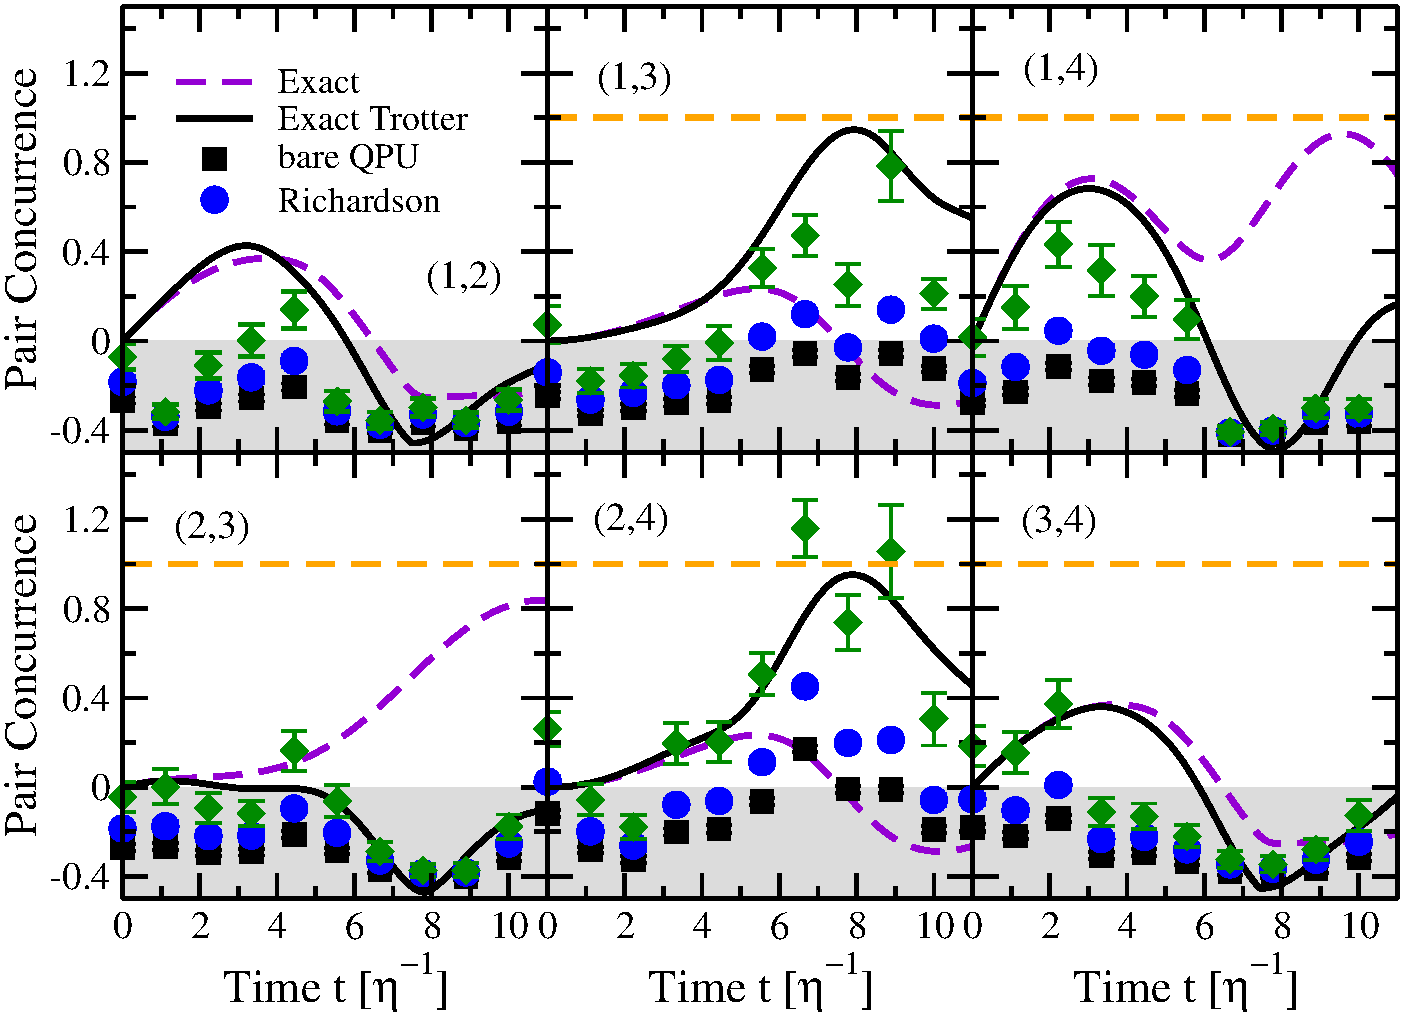
\includegraphics[width=0.49\textwidth]{conc_allpairs.pdf}
 \caption{(Color online) Entanglement concurrence for all the pairs of qubits. The maximum value for the concurrence is shown as a dashed orange line.}
\label{fig:conc_pair_1}
\end{figure}

\section{Conclusion}
\label{sec:conclusion}

In this chapter, we presented the first digital quantum simulation of the flavor dynamics in collective neutrino oscillations using current quantum technology. The results reported for the evolution of flavor and entanglement properties of a system with $N=4$ neutrino amplitudes show that current quantum devices based on superconducting qubits are starting to become a viable option for studying out-of-equilibrium dynamics of interacting many-body systems. The reduced fidelity in the results obtained here, compared to the simulations reported previously in \cite{Roggero_nptodg} employing the same quantum processor and a comparable number of entangling gates, points to the importance of controlling unitary errors associated with the imperfect implementation of arbitrary single-qubit rotations (on average $<1\%$ for the device used in both works). In future work we plan to explore the use of more advanced error mitigation strategies, such as Pauli twirling~\cite{Wallman2016} or symmetry protection~\cite{Tran2021}, to achieve a better overall fidelity.

We showed the zero-noise error extrapolation using a shifted Gaussian ansatz to be remarkably efficient in predicting the expected error-free estimator of observables. Given the large circuits employed in this section, past experience with zero-noise extrapolations (see e.g. \cite{roggero2020A,Roggero_nptodg}) suggest the exponential ansatz to be appropriate due to the large noise rates, and we find it to indeed outperforms Richardson extrapolation in this regime. The current results highlight the importance of using alternative measures of entanglement to the entropy in order to extract reliable information about quantum correlations in the states generated on the quantum device. Using the pair concurrence together with the entropy provides a robust way to detect entanglement even in the presence of substantial noise, like in the results shown here. We expect these insights, and the mapping of the neutrino evolution problem into a swap network, to prove very valuable in future explorations of out-of-equilibrium neutrino dynamics with near-term, noisy, quantum devices.

\chapter{Quantum Circuit Squeezing Algorithm}
\label{chap:qcsa}

\section{Introduction}

The quantum circuit squeezing algorithm (QCSA) is a novel quantum algorithm developed in this thesis which compresses the depth of a quantum circuit, with the trade-off of increased qubit size and required runs. The algorithm relies on two fundamental properties of maximally entangled states: the ricochet property and entanglement swapping. QCSA uses the combination of these two properties to replace horizontal lines of gates on a set of qubits to a vertical line of gates on a larger set of qubits.

\section{Maximal Entanglement}

QCSA relies extensively on maximally entangled states, a state whose entanglement entropy is maximal. A state $\ket{\psi}$ is maximally entangled if the partial trace of its density matrix $\rho=\ket{\psi}\bra{\psi}$ is equal to a multiple of the identity $I$; mathematically
\begin{align}
\text{Tr}_A\rho_{AB}=cI_B
,\end{align}
where $c$ is a constant. The partial trace can be defined as follows: Let $\{\ket{a_i}\}$ and $\{\ket{b_i}\}$ be the bases of Hilbert spaces $H_A$ and $H_B$, respectively. Let $\rho_{AB}\in H_A\otimes H_B$ be a density matrix which can be decomposed as
\begin{align}
\rho_{AB}=\sum_{ijkl}c_{ijkl}\ket{a_i}\bra*{a_j}\otimes\ket{b_k}\bra{b_l}
,\end{align}
where $c_{ijkl}$ are constants. Then the partial trace over $A$ is given by
\begin{align}
\text{Tr}_A(\rho_{AB})
&=\sum_{ijklm}c_{ijkl}\bra{a_m}\ket{a_i}\bra{a_j}\ket{a_m}\otimes\ket{b_k}\bra{b_l}
\\
&=\sum_{ijklm}c_{ijkl}\bra{a_j}\ket{a_m}\bra{a_m}\ket{a_i}\otimes\ket{b_k}\bra{b_l}
\\
&=\sum_{ijkl}c_{ijkl}\bra{a_j}\ket{a_i}\otimes\ket{b_k}\bra{b_l}.
\end{align}
One orthonormal set of maximally entangled states for two qubits, is the Bell state basis. It contains the following four states
\begin{align}
\ket{\phi^{\pm}} 
&=
\frac{1}{\sqrt{2}}\left(\ket{00}\pm\ket{11}\right)
\\
\ket{\psi^{\pm}} 
&=
\frac{1}{\sqrt{2}}\left(\ket{01}\pm\ket{10}\right),
\end{align}
which can be prepared on a quantum computer with the following short-depth circuit
\begin{align}
\label{Bell state circuit}
\Qcircuit @C=1.5em @R=1em 
{
\lstick{\ket{q_0}} & \gate{H} & \ctrl{1} & \qw \\
\lstick{\ket{q_1}} & \qw      & \targ    & \qw \\
} 
,\end{align}
where the initial state of the pair of qubits $\ket{q_0q_1}$ leads to the different Bell states as follows
\begin{align}
\ket{00} &\to \ket{\phi^+}, \\
\ket{10} &\to \ket{\phi^-}, \\
\ket{01} &\to \ket{\psi^+}, \\
\ket{11} &\to \ket{\psi^-}.
\end{align}
Each Bell state is maximally entangled because the partial trace of its density matrix is $I/2$. Note that preparing any of the initial states $\ket{q_0q_1}$ listed above does not increase the depth of the circuit as their preparation requires at most the application of a column of two $X$ gates, the top of which can be combined with the $H$ gate to form a single-qubit gate and the bottom of which can be executed in parallel with this new single-qubit gate. The notion of a maximally entangled state can be expanded to $n$ qubits. One such state is what we'll call the generalized Bell state $\ket{\phi_n^+}$ and it is defined as
\begin{align}
\label{phi_n_plus}
\ket{\phi_n^+}=\frac{1}{\sqrt{2^n}}\sum_{x\in h_n}\ket{xx}
,\end{align}
where $h_n=\{x \ | \ l(x)=n\}$ is the set of all bitstrings of length $n$. The states formed from this set $H_n = \{\ket{x} \ | \ x\in h_n\}$, which we'll call the bit-string states, are an orthonormal basis for the Hilbert space of $n$-qubits. The state $\ket{\phi^+_n}$ can be prepared with the following circuit of depth two:
\begin{align}
\label{u_gen}
\begin{centering}
\Qcircuit @C=1em @R=1em 
{
\lstick{\ket{0_1}} & \gate{H} & \ctrl{5} & \qw      & \qw      & \qw  
\\
\lstick{\ket{0_2}} & \gate{H} & \qw      & \ctrl{5} & \qw      & \qw
\\
\lstick{\vdots}
\\
\lstick{\ket{0_n}} & \gate{H} & \qw      & \qw      & \ctrl{5} & \qw
\\
\\
\lstick{\ket{0_{n+1}}} & \qw      & \targ    & \qw      & \qw      & \qw
\\
\lstick{\ket{0_{n+2}}} & \qw      & \qw      & \targ    & \qw      & \qw
\\
\lstick{\vdots}
\\
\lstick{\ket{0_{2n}}} & \qw      & \qw     & \qw      & \targ     & \qw
}     
\end{centering}
\end{align}
where the column of $n$ Hadamard gates $H$ places the top half of the qubits in the equal superposition of the states of $H_n$ while the ladder of CNOT gates "copies" each state of the top half of the qubits to the state of the bottom half, maximally entangling the two sets of qubits. The circuit is depth two because all of the CNOT gates can be run in parallel as they each act on disjoint pairs of qubits. Note that this is simply $n$ copies of the quantum circuit that prepares $\ket{\phi^+}$, (\ref{Bell state circuit}) with $\ket{q_0q_1}=\ket{00}$. The proof of the maximum entanglement of $\ket{\phi_n^+}$ is given below:
\begin{align}
\text{Tr}_A
\left(
\ket{\phi^+}\bra{\phi^+}
\right)
&=
\text{Tr}_A
\left(
\frac{1}{2^n}
\sum_{x,y\in h_n}\ket{xx}\bra{yy}
\right)
\nonumber
\\
&=
\frac{1}{2^n}
\sum_{x,y\in h_n}\bra{x}\ket{y}\ket{x}\bra{y}
\nonumber
\\
&=
\frac{1}{2^n}
\sum_{x,y\in h_n}\delta_{xy}\ket{x}\bra{y}
\nonumber
\\
&=
\frac{1}{2^n}
\sum_{x\in h_n}\ket{x}\bra{x}
\nonumber
\\
&=
\frac{1}{2^n}I
.\end{align}

The maximally entangled states introduced here serve as the building blocks for QCSA. We will now discuss the two properties of maximally entangled states that will be used to build the algorithm

\section{Ricochet Property}

The first property of maximally entangled states that will be used in QCSA is the Ricochet property. It states that, for any $n$-qubit gate $A$, the following equality holds
\begin{align}
\label{ricochet_definiton}
(A\otimes I)\ket{\phi_n^+} = (I\otimes A^T)\ket{\phi_n^+}
,\end{align} 
where one will recall $\ket{\phi_n^+}$ to be our previously defined (\ref{phi_n_plus}) maximally entangled state for $n$ qubits. The ricochet property can be proven as follows: First, write $A$ in terms of the orthonormal basis of $n$-qubits $H_n$ (which was defined as the set of all possible bit-string states of length $n$)
\begin{align}
A = \sum_{i,j\in h_n}^na_{ij}\ket{i}\bra{j},
\end{align}
where $a_{ij}$ are the matrix element of $A$. Then, plug this rewriting of $A$ into the left hand side (LHS) of the ricochet property definition (\ref{ricochet_definiton})
\begin{align}
\label{ricochet_proof}
\left(A\otimes I\right)\ket{\phi_n^+}
&=\frac{1}{\sqrt{n}}\sum_{ijk}^na_{ij}(\ket{i}\bra{j}\otimes I)\ket{kk} \\
&=\frac{1}{\sqrt{n}}\sum_{ij}^na_{ij}\ket{ij} \nonumber \\
&=\frac{1}{\sqrt{n}}\sum_{ijk}^na_{ij}(I\otimes\ket{j}\bra{i})\ket{kk} \nonumber  \\
&=\left(I\otimes A^T\right)\ket{\phi_n^+}.
\end{align}
The ricochet property for single qubit gates can be expressed via quantum circuits as:
\begin{align}
\begin{centering}
\Qcircuit @C=0.75em @R=.7em 
{
\push{\rule{0em}{1em}} & \lstick{\ket{0}} & \gate{H} & \ctrl{1} & \gate{A} & \qw  & & & & & &
\lstick{\ket{0}} & \gate{H} & \ctrl{1} & \qw & \qw & \qw 
\\
\push{\rule{0em}{1em}} & \lstick{\ket{0}} & \qw & \targ \qw & \qw & \qw & & \raisebox{2em}{=} & &
& &
\lstick{\ket{0}} & \qw & \targ & \qw & \gate{A^T} & \qw
}     
\end{centering}
\end{align}
The key insight here is that one can use this property to change two gates applied in series on a single qubit to two gates applied in parallel on two qubits. This process, which we'll call squeezing, can be seen in terms of quantum circuits below
\begin{align}
\begin{centering}
\Qcircuit @C=0.75em @R=.7em 
{
\push{\rule{0em}{1em}} & \lstick{\ket{0}} & \gate{H} & \ctrl{1} & \gate{B} & \gate{A} & \qw & & & & &
\lstick{\ket{0}} & \gate{H} & \ctrl{1} & \gate{A} & \qw 
\\
\push{\rule{0em}{1em}} & \lstick{\ket{0}} & \qw & \targ & \qw & \qw & \qw & \raisebox{2em}{=} & &
& &
\lstick{\ket{0}} & \qw & \targ & \gate{B^T} & \qw
}     
\end{centering}
,\end{align}
or, mathematically
\begin{align}
(AB\otimes I)\ket{\phi_n^+} 
&=(A\otimes I)\left[(B\otimes I)\ket{\phi_n^+}\right]  \\
&=(A\otimes I)\left[(I\otimes B^T)\ket{\phi_n^+}\right] \nonumber \\
&=(A\otimes B^T)\ket{\phi_n^+} \nonumber
.\end{align}
The ricochet property for the $n$-qubit case, using $\ket{\phi_n^+}$ can be visualized in terms of quantum circuits as follows
\begin{align}
\begin{centering}
\Qcircuit @C=1em @R=1em 
{
\lstick{\ket{0}} & \gate{H} & \ctrl{5} & \qw      & \qw      & \multigate{3}{A}   & \qw
& & & &
\lstick{\ket{0}} & \gate{H} & \ctrl{5} & \qw      & \qw      & \qw                & \qw
\\
\lstick{\ket{0}} & \gate{H} & \qw      & \ctrl{5} & \qw      & \ghost{A}          & \qw
& & & &
\lstick{\ket{0}} & \gate{H} & \qw      & \ctrl{5} & \qw      & \qw                & \qw
\\
\lstick{\vdots}
\\
\lstick{\ket{0}} & \gate{H} & \qw      & \qw      & \ctrl{5} & \ghost{A}          & \qw
& & & &
\lstick{\ket{0}} & \gate{H} & \qw      & \qw      & \ctrl{5} & \qw                & \qw
\\
                 &          &          &          &          &     &                    &
& \raisebox{0em}{=}
\\
\lstick{\ket{0}} & \qw      & \targ    & \qw      & \qw      & \qw                & \qw
& & & &
\lstick{\ket{0}} & \qw      & \targ    & \qw      & \qw      & \multigate{3}{A^T} & \qw
\\
\lstick{\ket{0}} & \qw      & \qw      & \targ    & \qw      & \qw                & \qw
& & & &
\lstick{\ket{0}} & \qw      & \qw      & \targ    & \qw      & \ghost{A^T}        & \qw
\\
\lstick{\vdots}
\\
\lstick{\ket{0}} & \qw      & \qw     & \qw      & \targ     & \qw                & \qw
& & & &
\lstick{\ket{0}} & \qw      & \qw     & \qw      & \targ     & \ghost{A^T}        & \qw
}     
\end{centering}
,\end{align}
and the squeezing process can additionally be visualized as
\begin{align}
\begin{centering}
\Qcircuit @C=1em @R=1em 
{
\lstick{\ket{0}} & \gate{H} & \ctrl{5} & \qw      & \qw      & \multigate{3}{B}   & \multigate{3}{A}   & \qw
& & & &
\lstick{\ket{0}} & \gate{H} & \ctrl{5} & \qw      & \qw      & \multigate{3}{A}   & \qw
\\
\lstick{\ket{0}} & \gate{H} & \qw      & \ctrl{5} & \qw      & \ghost{B}          & \ghost{A}          & \qw
& & & &
\lstick{\ket{0}} & \gate{H} & \qw      & \ctrl{5} & \qw      & \ghost{A}          & \qw
\\
\lstick{\vdots}
\\
\lstick{\ket{0}} & \gate{H} & \qw      & \qw      & \ctrl{5} & \ghost{B}          & \ghost{A}          & \qw
& & & &
\lstick{\ket{0}} & \gate{H} & \qw      & \qw      & \ctrl{5} & \ghost{A}          & \qw
\\
                 &          &          &          &          &                    &                    &
& \raisebox{0em}{=}
\\
\lstick{\ket{0}} & \qw      & \targ    & \qw      & \qw      & \qw                & \qw                & \qw
& & & &
\lstick{\ket{0}} & \qw      & \targ    & \qw      & \qw      & \multigate{3}{B^T} & \qw
\\
\lstick{\ket{0}} & \qw      & \qw      & \targ    & \qw      & \qw                & \qw                & \qw
& & & &
\lstick{\ket{0}} & \qw      & \qw      & \targ    & \qw      & \ghost{B^T}        & \qw
\\
\lstick{\vdots}
\\
\lstick{\ket{0}} & \qw      & \qw     & \qw      & \targ     & \qw                & \qw                & \qw
& & & &
\lstick{\ket{0}} & \qw      & \qw     & \qw      & \targ     & \ghost{B^T}        & \qw
}     
\end{centering}
\end{align}
So far, we've only been able to squeeze (reduce) our circuit depth by a factor 2. In order to do better, we'll need to introduce the second property of maximally entangled states upon which QCSA relies.

\section{Entanglement swapping}

The property of maximally entangled states that allows one to extend the benefits of the ricochet property to be able to squeeze the depth of a circuit by more than half is called entanglement swapping. To express it mathematically, let me first introduce the notation $\ket{\phi^n_{ab}}$ to mean that the generalized Bell state $\ket{\phi_n^+}$ (\ref{phi_n_plus}) is applied to qubit sets $a$ and $b$; that is
\begin{align}
\label{gen_bell}
\ket{\phi^n_{ab}}=\frac{1}{\sqrt{2^n}}\sum_{x\in h_n}\ket{x_ax_b}
,\end{align}
where $h_n=\{x \ | \ l(x)=n\}$ is the set of all bitstrings of length $n$, while $a$ and $b$ are sets of $n$-qubits. For example, for $n=2$, $a=\{0,1\}$, and $b=\{2,3\}$, we would have $h_n=\{00,01,10,11\}$ and the generalized Bell state would be
\begin{align}
\ket{\phi^n_{ab}}
=
\frac{1}{\sqrt{2^2}}\sum_{x\in h_2}\ket*{x_{\{0,1\}}x_{\{2,3\}}}
=
\frac{1}{2}
\left(
\ket{0000}+\ket{0101}+\ket{1010}+\ket{1111}
\right)
.\end{align}
With this notation in hand, the entanglement swapping property can then be stated as follows:
\begin{align}
\label{ent_swap_prop}
\bra{\phi^n_{bc}}\ket{\phi^n_{ab}\phi^n_{cd}}
=
\frac{1}{2^n}
\ket{\phi^n_{ad}}
,\end{align}
which can be proven by inserting into it the definition of the generalized Bell state (\ref{gen_bell}) which yields
\begin{align}
\bra{\phi^n_{bc}}\ket{\phi^n_{ab}\phi^n_{cd}}
&=
\left(
\frac{1}{\sqrt{2^n}}\sum_{x\in h_n}\bra{x_bx_c}
\right)
\left(
\frac{1}{2^n}\sum_{y,z\in h_n}\ket{y_ay_bz_cz_d}
\right)
\\
&=
\frac{1}{\sqrt{2^{3n/2}}}
\sum_{x\in h_n}
\ket{y_a}\bra{x_b}\ket{y_b}\bra{x_c}\ket{z_c}\ket{z_d}
\nonumber
\\
&=
\frac{1}{\sqrt{2^{3n/2}}}
\sum_{x\in h_n}
\delta_{xy}\delta_{xz}
\ket{y_a}\ket{z_d}
\nonumber
\\
&=
\frac{1}{2^n}
\left(
\frac{1}{\sqrt{2^n}}
\sum_{x\in h_n}
\ket{x_ax_d}
\right)
\nonumber
\\
&=
\frac{1}{2^n}
\ket{\phi^n_{ad}}
.\end{align}
Taking the complex conjugate squared of both sides of the entanglement swapping property (\ref{ent_swap_prop}) 
\begin{align}
\abs{\bra{\phi^n_{bc}}\ket{\phi^n_{ab}\phi^n_{cd}}}^2
=
\frac{1}{4^n}
\bra{\phi^n_{ad}}\ket{\phi^n_{ad}}
=
\frac{1}{4^n}
,\end{align}
implies that the probability of measuring qubit sets $b$ and $c$ to be in the state $\ket{\phi^+_n}$ is $1/4^n$. One can test whether qubit sets $b$ and $c$ are in the state $\ket{\phi^+_n}$ by applying $(U^n_{bc})^\dagger$ to said qubits, measure them, and check if they were both measured to be in the all zero state $\ket{0}^{\otimes n}$. Here, we've defined $U^n_{ab}$ as the quantum gate that takes qubit sets $a$ and $b$ from the all zero state to the generalized Bell state $\ket{\phi^n_{ab}}$; that is
\begin{align}
\label{unab_def}
U_{n}\ket{0}^{\otimes n}_a\ket{0}^{\otimes n}_b = \ket{\phi^n_{ab}}
.\end{align}
To get a better feel for the entanglement swapping property, we show here the property in terms of quantum circuits for the $n=1$ case:
\begin{align}
\label{small_circ}
\Qcircuit @C=1em @R=1em 
{
\lstick{\ket{0_a}} & \gate{H} & \ctrl{1} & \qw      & \qw      & \qw    & \qw     & & &                  & \lstick{\ket{0_a}} & \gate{H} & \ctrl{3} & \qw \\
\lstick{\ket{0_b}} & \qw      & \targ    & \ctrl{1} & \gate{H} & \meter & \qw \\
\lstick{\ket{0_c}} & \gate{H} & \ctrl{1} & \targ    & \qw      & \meter & \qw    & \raisebox{2em}{$\xrightarrow[]{1/4}$} \\
\lstick{\ket{0_d}} & \qw      & \targ    & \qw      & \qw      & \qw    & \qw    & & &                  & \lstick{\ket{0_d}} & \qw      & \targ    & \qw \\
} 
,\end{align}
whose mathematical description matches that of the $n=1$ case of the definition of the property \ref{ent_swap_prop}
\begin{align}
\bra{00}(U^n_{bc})^\dagger U^n_{ab}U^n_{bc}\ket{0000}
&=
\frac{1}{2^n}
\ket{\phi^n_{ad}}
\\
\bra{\phi^n_{bc}}\ket{\phi^n_{ab}\phi^n_{cd}}
&=
\frac{1}{2^n}
\ket{\phi^n_{ad}}
,\end{align}
where we've used the definition \ref{unab_def}. Here the arrow with $1/4$ above it from \ref{small_circ} implies that qubits $b$ and $c$ were measured to be $00$ with probability $1/4$. Additionally, qubits $b$ and $c$ have been discarded in the circuit to the right of the arrow as they have been measured and are therefore no longer relevant. Note that, in the $n=1$ case considered above $U^n_{xy}$ is simply the quantum circuit that prepares $\ket{\phi^+}$ given in \ref{Bell state circuit} (with $x=q_0$ and $y=q_1$); that is, a Hadamard applied to the top qubit $x$ and a CNOT with the qubits $x$ and $y$ being the control and target qubits, respectively. We'll now consider the arbitrary $n$ case (\ref{ent_swap_prop}). Here, $U^n_{xy}$ is the quantum circuit given in (\ref{u_gen}). This case is given in the quantum circuit representation below, in which the arrow with a $\frac{1}{4^n}$ above it, implying that the qubit sets $b$ and $c$ were measured to be in the all zero state $\ket{0\ldots 0}$:
\begin{align}
\label{n_qubit_ent_swap}
\begin{centering}
\Qcircuit @C=1em @R=1em 
{
&& \lstick{\ket{0}} & \gate{H} & \ctrl{4} & \qw      & \qw \barrier{15} & \qw        & \qw  & \qw & \qw & \qw
& & & & &
\lstick{\ket{0}} & \gate{H} & \ctrl{12} & \qw     & \qw              & \qw 
\\
&& \lstick{\ket{0}} & \gate{H} & \qw      & \ctrl{4} & \qw      & \qw     & \qw      & \qw   & \qw & \qw
& & & & &
\lstick{\ket{0}} & \gate{H} & \qw      & \ctrl{12}& \qw             & \qw
\\
&& \lstick{\vdots}
\\
&& \lstick{\ket{0}} & \gate{H} & \qw      & \qw      & \ctrl{4} & \qw     & \qw      & \qw   & \qw & \qw
& & & & &
\lstick{\ket{0}} & \gate{H} & \qw      & \qw      & \ctrl{12} & \qw
\\
&& \lstick{\ket{0}} & \qw      & \targ    & \qw      & \qw      & \ctrl{4} & \qw     & \qw  & \gate{H} & \meter
\\
&& \lstick{\ket{0}} & \qw      & \qw      & \targ    & \qw      & \qw     & \ctrl{4} & \qw  & \gate{H} & \meter 
\\
&& \lstick{\vdots}
\\
&& \lstick{\ket{0}} & \qw      & \qw     & \qw      & \targ     & \qw     & \qw      & \ctrl{4} & \gate{H} & \meter
& & \raisebox{-3em}{$\xrightarrow[]{\frac{1}{4^n}}$}
\\
&& \lstick{\ket{0}} & \gate{H} & \ctrl{4} & \qw      & \qw      & \targ   & \qw      & \qw      & \qw      & \meter
\\
&& \lstick{\ket{0}} & \gate{H} & \qw      & \ctrl{4} & \qw      & \qw     & \targ      & \qw    & \qw      & \meter
\\
&& \lstick{\vdots}
\\
&& \lstick{\ket{0}} & \gate{H} & \qw      & \qw      & \ctrl{4} & \qw    & \qw         & \targ  & \qw      & \meter
\\
&& \lstick{\ket{0}} & \qw      & \targ    & \qw      & \qw     & \qw & \qw & \qw & \qw & \qw 
& & & & &
\lstick{\ket{0}} & \qw      & \targ    & \qw      & \qw     & \qw
\\
&& \lstick{\ket{0}} & \qw      & \qw      & \targ    & \qw     & \qw & \qw & \qw & \qw & \qw 
& & & & &
\lstick{\ket{0}} & \qw      & \qw      & \targ    & \qw     & \qw
\\
&& \lstick{\vdots}
\\
&& \lstick{\ket{0}} & \qw      & \qw     & \qw      & \targ   & \qw & \qw & \qw & \qw & \qw 
& & & & &
\lstick{\ket{0}} & \qw      & \qw     & \qw      & \targ   & \qw 
\inputgroupv{1}{4}{1.5em}{2.5em}{a}
\inputgroupv{5}{8}{1.5em}{2.5em}{b}
\inputgroupv{9}{12}{1.5em}{2.5em}{c}
\inputgroupv{13}{16}{1.5em}{2.5em}{d}
}     
\end{centering}
\end{align}

\section{Dicke Subspace Modification}
\label{sec:subspace_mod}

The quantum circuit squeezing algorithm can be modified for circuits that preserve Hamming weight (for example, ansatzes in second quantization for systems that preserve particle number) so that the increase in additional measurements is reduced. To describe this modification, let us first define what we'll call the Dicke-Bell state $\ket*{\phi^n_k}$, which can be thought of as a maximally entangled state in the sub-space of the Hilbert space for $n$ qubits containing only the bit-string states that have a Hamming weight of $k$. Mathematically
\begin{align}
\label{dicke_bell}
\ket{\phi^n_k}
=
\frac{1}{\sqrt{{n \choose k}}}
\sum_{x\in h^n_k}\ket{xx}
,\end{align}
where $h^n_k=\{x \ | \ \text{l}(x)=n, \text{wt}(x)=k\}$; that is the set of all bit-strings $x$ with length $n$ and Hamming weight $k$. For example,
\begin{align}
\ket{\phi^4_2}
= \ &
\frac{1}{\sqrt{6}}
(
\ket{1100}\otimes\ket{1100}
+
\ket{1010}\otimes\ket{1010}
+
\ket{1001}\otimes\ket{1001}
\\
+ \ &
\ket{0110}\otimes\ket{0110}
+
\ket{0101}\otimes\ket{0101}
+
\ket{0011}\otimes\ket{0011}
)
.\end{align}
It is analogous to the state $\ket{\phi^+_n}$ defined in (\ref{phi_n_plus}) with $x$ being drawn from the set $h^n_k$ instead of $h_n$. The states created from the latter, $H_n = \{\ket{x} \ | x\in h_n\}$, are an orthonormal basis for the Hilbert space of $n$-qubits. This is as opposed to the states created from the former, $H^n_k = \{\ket{x} \ | x\in h^n_k\}$, which is an orthonormal basis for $H^n_k$, the subset of the Hilbert space for $n$-qubits containing only quantum states formed from bit-string states with a Hamming weight of $k$. The Dicke-Bell state $\ket*{\phi^n_k}$ can be formed from the following circuit
\begin{align}
\begin{centering}
\Qcircuit @C=1em @R=1em 
{
\lstick{\ket{0}} & \multigate{3}{U^n_k} & \ctrl{5} & \qw      & \qw & \qw
\\
\lstick{\ket{0}} & \ghost{U^n_k}  & \qw      & \ctrl{5} & \qw & \qw
\\
\lstick{\vdots}
\\
\lstick{\ket{0}} & \ghost{U^n_k} & \qw      & \qw      & \ctrl{5} & \qw
\\
\\
\lstick{\ket{0}} & \qw      & \targ    & \qw      & \qw      & \qw  
\\
\lstick{\ket{0}} & \qw      & \qw      & \targ    & \qw      & \qw 
\\
\lstick{\vdots}
\\
\lstick{\ket{0}} & \qw      & \qw     & \qw      & \targ     & \qw 
}     
\end{centering}
,\end{align}
where $U^n_k$ takes the $n$-qubit all-zero state to the $n,k$ Dicke state; that is
\begin{align}
U^n_k\ket{0}^{\otimes n}=\ket*{D^n_k}
,\end{align}
where the Dicke state $\ket*{D^n_k}$ is defined as the equal superposition of all bit-string states of length $n$ and Hamming weight $k$; that is
\begin{align}
\ket*{D^n_k}
=
\frac{1}{\sqrt{{n \choose k}}}
\sum_{x\in h^n_k}\ket{xx}    
.\end{align}
The reason we've named the resulting state the Dicke-Bell state is now revealed; it is the entanglement of a Dicke-state into a maximally entangled state for a constant Hamming weight subspace. Finding a short-depth circuit decomposition for $U^n_k$ (to prepare a Dicke state) is an active area of research. It has been shown how to construct $U^n_k$ with $\mathcal{O}(n)$ depth and $\mathcal{O}(kn)$ gates (\cite{ref:dicke_prep} and \cite{ref:dicke_prep_dac}). While linear depth is certainly not as good as the constant two depth circuits (\ref{u_gen}) we shall see that using the subspace modification (which requires the preparation of Dicke states) provides a significant advantage in terms of amount of shots (runs of quantum circuits) required. Additionally, more efficient preparation methods may be discovered, including the method considered in chapter \ref{vpds}. 

It can be shown that the ricochet property still holds for $\ket*{\phi^n_k}$. That is, for any $n$ by $n$ matrix $A_k$ that preserves the Hamming weight ($k$) of any state upon which it acts, the following equality holds
\begin{align}
(A\otimes I)\ket{\phi^n_k} = (I\otimes A^T)\ket{\phi^n_k}
.\end{align}
It can be proven analogously to the proof of the original ricochet property (\ref{ricochet_proof}) by writing $A$ in terms of the orthonormal basis $h^n_k$
\begin{align}
A_k = \sum_{x,y\in h^n_k}a_{xy}\ket{x}\bra{y}
,\end{align}
and calculating
\begin{align}
\left(A_k\otimes I\right)\ket{\phi^n_k}
&=\frac{1}{\sqrt{{n \choose k}}}\sum_{xyz}a_{xy}(\ket{x}\bra{y}\otimes I)\ket{zz} \\
&=\frac{1}{\sqrt{{n \choose k}}}\sum_{xy}a_{xy}\ket{xy} \nonumber \\
&=\frac{1}{\sqrt{{n \choose k}}}\sum_{xyz}a_{xy}(I\otimes\ket{y}\bra{x})\ket{zz} \nonumber  \\
&=\left(I\otimes A_k^T\right)\ket{\phi^n_k} \nonumber
,\end{align}
where $x,y,z$ sum over the set $h^n_k$. The quantum circuit representation of this ricochet property is given below
\begin{align}
\begin{centering}
\Qcircuit @C=1em @R=1em 
{
\lstick{\ket{0}} & \multigate{3}{U^n_k} & \ctrl{5} & \qw      & \qw      & \multigate{3}{A}   & \qw
& & & &
\lstick{\ket{0}} & \multigate{3}{U^n_k} & \ctrl{5} & \qw      & \qw      & \qw                & \qw
\\
\lstick{\ket{0}} & \ghost{U^n_k}  & \qw      & \ctrl{5} & \qw      & \ghost{A}          & \qw
& & & &
\lstick{\ket{0}} & \ghost{U^n_k}  & \qw      & \ctrl{5} & \qw      & \qw                & \qw
\\
\lstick{\vdots}
\\
\lstick{\ket{0}} & \ghost{U^n_k} & \qw      & \qw      & \ctrl{5} & \ghost{A}          & \qw
& & & &
\lstick{\ket{0}} & \ghost{U^n_k} & \qw      & \qw      & \ctrl{5} & \qw                & \qw
\\
                 &          &          &          &          &     &                    &
& \raisebox{0em}{=}
\\
\lstick{\ket{0}} & \qw      & \targ    & \qw      & \qw      & \qw                & \qw
& & & &
\lstick{\ket{0}}   & \qw      & \targ    & \qw      & \qw      & \multigate{3}{A^T} & \qw
\\
\lstick{\ket{0}} & \qw      & \qw      & \targ    & \qw      & \qw                & \qw
& & & &
\lstick{\ket{0}} & \qw      & \qw      & \targ    & \qw      & \ghost{A^T}        & \qw
\\
\lstick{\vdots}
\\
\lstick{\ket{0}} & \qw      & \qw     & \qw      & \targ     & \qw                & \qw
& & & &
\lstick{\ket{0}} & \qw      & \qw     & \qw      & \targ     & \ghost{A^T}        & \qw
}     
\end{centering}
\end{align}
Because $A_k$ preserves Hamming weight, it sees the subspace $H^n_k$ the same way that $A$ sees $H^n$, as the entire space that it can explore. In other words, $H^n_k$ is closed under the application of $A_k$ just as $H^n$ is closed under the application of $A$. Mathematically, $\forall x\in H^n_k$, $A_kx\in H^n_k$ just as $\forall x\in H_n$, $Ax\in H_n$. 

Entanglement swapping also holds for $\ket*{\phi^n_k}$. To explain it, let me first introduce the notation $\ket*{\phi^{nk}_{ij}}$ to mean that the state Dicke-Bell state $\ket*{\phi^n_k}$ is applied to qubits $i$ and $j$; that is
\begin{align}
\label{dicke-bell-nkij}
\ket{\phi^{nk}_{ij}} = \frac{1}{\sqrt{{n \choose k}}}\sum_{x \in h^n_k}\ket{x_ix_j}.
\end{align}
Then, the analogous entanglement swapping property is
\begin{align}
\label{ent_swap_analoug}
\bra{\phi^{nk}_{bc}}\ket{\phi^{nk}_{ab}\phi^{nk}_{cd}}
=
\frac{1}{{n \choose k}}\ket{\phi^{nk}_{ad}},
,\end{align}
which can be proven by inserting into it the definition of the Dicke-Bell state (\ref{dicke-bell-nkij}) which yields
\begin{align}
\bra{\phi^{nk}_{bc}}\ket{\phi^{nk}_{ab}\phi^{nk}_{cd}}
&=
\left(
\frac{1}{\sqrt{{n \choose k}}}
\sum_{x\in h^n_k}\bra{x_bx_c}
\right)
\left(
\frac{1}{{n \choose k}}
\sum_{y,z\in h^n_k}\ket{y_ay_bz_cz_d}
\right)
\\
&=
\frac{1}{{n \choose k}^{3/2}}
\sum_{x,y,z\in h^n_k}\ket{y_a}\bra{x_b}\ket{y_b}\bra{x_c}\ket{y_c}\ket{z_d}
\\
&=
\frac{1}{{n \choose k}^{3/2}}
\sum_{x,y,z\in h^n_k}\delta_{xy}\delta_{xz}\ket{y_a}\ket{z_d}
\\
&=
\frac{1}{{n \choose k}}
\left(
\frac{1}{\sqrt{{n \choose k}}}
\sum_{x\in h^n_k}\ket{x_a}\ket{x_d}
\right)
\\
&=
\frac{1}{{n \choose k}}\ket{\phi^{nk}_{ad}}
.\end{align}
Note that the probability of success (every qubit in the qubit sets $b$ and $c$ was measured to be zero) has gone from scaling exponentially with $n$ (\ref{ent_swap_prop}) to scaling linearly with $n$ (\ref{ent_swap_analoug}), the benefits of which will become clear soon. The entanglement swapping property can be viewed in terms of quantum circuits below, in which the arrow with a $1/{n \choose k}^2$ above it meaning that the probability of success is $1/{n \choose k}^2$.

\begin{align}
\begin{centering}
\Qcircuit @C=1em @R=1em 
{
\lstick{\ket{0}} & \multigate{3}{U^n_k} & \ctrl{4} & \qw      & \qw \barrier{15} & \qw        & \qw  & \qw & \qw & \qw
& & & & &
\lstick{\ket{0}} & \multigate{3}{U^n_k} & \ctrl{12} & \qw     & \qw              & \qw 
\\
\lstick{\ket{0}} & \ghost{U^n_k} & \qw      & \ctrl{4} & \qw      & \qw     & \qw      & \qw   & \qw & \qw
& & & & &
\lstick{\ket{0}} & \ghost{U^n_k} & \qw      & \ctrl{12}& \qw             & \qw
\\
\lstick{\vdots}
\\
\lstick{\ket{0}} & \ghost{U^n_k} & \qw      & \qw      & \ctrl{4} & \qw     & \qw      & \qw   & \qw & \qw
& & & & &
\lstick{\ket{0}} & \ghost{U^n_k} & \qw      & \qw      & \ctrl{12} & \qw
\\
\lstick{\ket{0}} & \qw      & \targ    & \qw      & \qw      & \ctrl{4} & \qw     & \qw  & \multigate{3}{(U^n_k)^\dagger} & \meter
\\
\lstick{\ket{0}} & \qw      & \qw      & \targ    & \qw      & \qw     & \ctrl{4} & \qw  & \ghost{(U^n_k)^\dagger} & \meter 
\\
\lstick{\vdots}
\\
\lstick{\ket{0}} & \qw      & \qw     & \qw      & \targ     & \qw     & \qw      & \ctrl{4} & \ghost{(U^n_k)^\dagger} & \meter
& & \raisebox{-3em}{$\xrightarrow[]{\frac{1}{{n \choose k}^{2}}}$}
\\
\lstick{\ket{0}} & \multigate{3}{U^n_k} & \ctrl{4} & \qw      & \qw      & \targ   & \qw      & \qw      & \qw      & \meter
\\
\lstick{\ket{0}} & \ghost{U^n_k} & \qw      & \ctrl{4} & \qw      & \qw     & \targ      & \qw    & \qw      & \meter
\\
\lstick{\vdots}
\\
\lstick{\ket{0}} & \ghost{U^n_k} & \qw      & \qw      & \ctrl{4} & \qw    & \qw         & \targ  & \qw      & \meter
\\
\lstick{\ket{0}} & \qw      & \targ    & \qw      & \qw     & \qw & \qw & \qw & \qw & \qw 
& & & & &
\lstick{\ket{0}} & \qw      & \targ    & \qw      & \qw     & \qw
\\
\lstick{\ket{0}} & \qw      & \qw      & \targ    & \qw     & \qw & \qw & \qw & \qw & \qw 
& & & & &
\lstick{\ket{0}} & \qw      & \qw      & \targ    & \qw     & \qw
\\
\lstick{\vdots}
\\
\lstick{\ket{0}} & \qw      & \qw     & \qw      & \targ   & \qw & \qw & \qw & \qw & \qw 
& & & & &
\lstick{\ket{0}} & \qw      & \qw     & \qw      & \targ   & \qw 
}     
\end{centering}
\end{align}

\section{Entanglement Swapping Recursion}

As we've seen, the procedure of entanglement swapping can be used to reduce the length of a circuit by the order of a factor of two. However, we can further reduce the circuit length by extending entanglement swapping in a recursive manner: First, we define the base case:
\begin{align}
\bra{0}U^\dagger_{bc}U_{ab}U_{cd}\ket{0}
=
\sqrt{p}U_{ad}\ket{0}
,\end{align}
where
\begin{align}
U_{ab}\ket{0}=\ket{\phi_{ab}}
,\end{align}
with $\ket{\phi_{ab}}$ defined as a general maximally entangled state which is maximally entangled in some subspace $H$. We define it generally here so as to cover the previously explored cases: when $H=H^n$, the full Hilbert space of $n$ qubits, and when $H=H^n_k$, the subspace of $H^n$ restricted to states of Hamming weight $k$. (However, $H$ can be any subspace of $H^n$.) The state formed by applying $U_{ab}$ to the vacuum and the probability $p$ are determined by $H$. For example, when $H=H^n$, we have $U_{ab}\ket{0}=\ket*{\phi^n_{ab}}$ and $p=1/4^n$. Meanwhile, when $H=H^n_k$, we have $U_{ab}\ket{0}=\ket*{\phi^{nk}_{ab}}$ and $p=1/{n \choose k}^2$. This base case can be represented by the following quantum circuit diagram.
\begin{align}
\begin{centering}
\Qcircuit @C=1em @R=1em 
{
&& \lstick{\ket{0}} & \multigate{5}{U} & \qw                      & \qw    & & & \lstick{\ket{0}} & \multigate{11}{U} & \qw 
\\
&& \lstick{\vdots}  &                  &                          &        & & & \lstick{\vdots}
\\
&& \lstick{\ket{0}} & \ghost{U}        & \qw                      & \qw    & & & \lstick{\ket{0}} & \ghost{U} & \qw
\\
&& \lstick{\ket{0}} & \ghost{U}        & \multigate{5}{U^\dagger} & \meter  
\\
&& \lstick{\vdots}
\\
&& \lstick{\ket{0}} & \ghost{U}        & \ghost{U^\dagger}        & \meter
\\
&& \lstick{\ket{0}} & \multigate{5}{U} & \ghost{U^\dagger}        & \meter & \raisebox{3em}{$\xrightarrow[]{p}$} 
\\
&& \lstick{\vdots}
\\
&& \lstick{\ket{0}} & \ghost{U}        & \ghost{U^\dagger}        & \meter 
\\
&& \lstick{\ket{0}} & \ghost{U}        & \qw & \qw    & & & \lstick{\ket{0}} & \ghost{U}         & \qw
\\
&& \lstick{\vdots}  &                  &                          &        & & & \lstick{\vdots}
\\
&& \lstick{\ket{0}} & \ghost{U}        & \qw       & \qw    & & & \lstick{\ket{0}} & \ghost{U}         & \qw
\inputgroupv{1}{3}{1.5em}{1.5em}{a}
\inputgroupv{4}{6}{1.5em}{1.5em}{b}
\inputgroupv{7}{9}{1.5em}{1.5em}{c}
\inputgroupv{10}{12}{1.5em}{1.5em}{d}
}
\end{centering}
\end{align}
The recursive extension of entanglement swapping can be stated mathematically as
\begin{align}
\label{recursive_entanglement_swapping}
\bra{0}\prod_{k=1}^{N-1}U^\dagger_{2k-1,2k}\prod_{k=1}^{N}U_{2k-2,2k-1}\ket{0}
=
\sqrt{p^{N-1}}U_{0,2N-1}\ket{0},
\end{align}
where the indices of $U$ refer to qubit sets. To prove this, we assume as the induction hypothesis, that (\ref{recursive_entanglement_swapping}) is true and proceed to show that the statement holds when we take $N\to N+1$:
\begin{align}
\bra{0}\prod_{k=1}^{N}U^\dagger_{2k-1,2k}\prod_{k=1}^{N+1}U_{2k-2,2k-1}\ket{0};
\end{align}
pulling out the $k=N$ term from the first product and the $k=N$ and $k=N+1$ terms from the second product yields
\begin{align}
\bra{0}\prod_{k=1}^{N-1}U^\dagger_{2k-1,2k}\prod_{k=1}^{N-1}U_{2k-2,2k-1}\ket{0}
\bra{0}U^\dagger_{2N-1,2N}U_{2N-2,2N-1}U_{2N,2N+1}\ket{0};
\end{align}
using the base case yields
\begin{align}
\sqrt{p}
\bra{0}\prod_{k=1}^{N-1}U^\dagger_{2k-1,2k}\prod_{k=1}^{N-1}U_{2k-2,2k-1}\ket{0}
U_{2N-2,2N+1}\ket{0};
\end{align}
relabeling qubit set $2N+1\to2N-1$ (which is allowed as qubit set $2N-1$ has been measured) yields
\begin{align}
\bra{0}\prod_{k=1}^{N-1}U^\dagger_{2k-1,2k}\prod_{k=1}^{N}U_{2k-2,2k-1}\ket{0};
\end{align}
applying the induction hypothesis gives
\begin{align}
\sqrt{p^{N}}U_{0,2N-1}\ket{0}
\end{align}
which completes the proof. The quantum circuit representation of entanglement swapping recursion for the case $N=3$ is given below

\begin{align}
\begin{centering}
\Qcircuit @C=1em @R=1em 
{
\lstick{\ket{0}} & \multigate{5}{U}  & \qw                      & \qw    & & & \lstick{\ket{0}} & \multigate{11}{U} & \qw                      & \qw    & & & \lstick{\ket{0}} & \multigate{17}{U} & \qw
\\
\lstick{\vdots}  &                   &                          &        & & & \lstick{\vdots}  &                   &                          &        & & & \lstick{\vdots}
\\
\lstick{\ket{0}} & \ghost{U}        & \qw                      & \qw     & & & \lstick{\ket{0}} & \ghost{U}        & \qw                      & \qw     & & & \lstick{\ket{0}} & \ghost{U}        & \qw 
\\
\lstick{\ket{0}} & \ghost{U}        & \multigate{5}{U^\dagger} & \meter  
\\
\lstick{\vdots}
\\
\lstick{\ket{0}} & \ghost{U}        & \ghost{U^\dagger}        & \meter
\\
\lstick{\ket{0}} & \multigate{5}{U} & \ghost{U^\dagger}        & \meter & \raisebox{3em}{$\xrightarrow[]{p}$} 
\\
\lstick{\vdots}
\\
\lstick{\ket{0}} & \ghost{U}        & \ghost{U^\dagger}        & \meter 
\\
\lstick{\ket{0}} & \ghost{U}        & \multigate{5}{U^\dagger} & \qw    & & & \lstick{\ket{0}} & \ghost{U}        & \multigate{5}{U^\dagger} & \meter
\\
\lstick{\vdots}  &                  &                          &        & & & \lstick{\vdots}
\\
\lstick{\ket{0}} & \ghost{U}        & \ghost{U^\dagger}        & \qw    & & & \lstick{\ket{0}} & \ghost{U}        & \ghost{U^\dagger}        & \meter
\\ 
\lstick{\ket{0}} & \multigate{5}{U} & \ghost{U^\dagger}        & \qw    & & & \lstick{\ket{0}} & \multigate{5}{U} & \ghost{U^\dagger}       & \meter & \raisebox{3em}{$\xrightarrow[]{p}$}
\\
\lstick{\vdots}  &                  &                          &        & & & \lstick{\vdots}
\\
\lstick{\ket{0}} & \ghost{U}        & \ghost{U^\dagger}        & \qw    & & & \lstick{\ket{0}} & \ghost{U}         & \ghost{U^\dagger}        & \meter   
\\
\lstick{\ket{0}} & \ghost{U}        & \qw                      & \qw    & & & \lstick{\ket{0}} & \ghost{U}         & \qw                      & \qw    & & & \lstick{\ket{0}} & \ghost{U}         & \qw   
\\
\lstick{\vdots}  &                  &                          &        & & & \lstick{\vdots}  &                   &                          &        & & & \lstick{\vdots}
\\
\lstick{\ket{0}} & \ghost{U}        & \qw                      & \qw    & & & \lstick{\ket{0}} & \ghost{U}         & \qw                      & \qw    & & & \lstick{\ket{0}} & \ghost{U}         & \qw   
}
\end{centering}
\end{align}

\section{The Algorithm}

We will now combine everything introduced thus far (ricochet property, entanglement swapping property, and entanglement swapping recursion) in order to construct the quantum circuit squeezing algorithm (QCSA). Before we give a formal definition, we'll walk through the algorithm for single-qubit gates and a single recursion step in quantum circuit form: Let $A,B,C,D$ be arbitrary single qubit gates. Then the QCSA circuit is given by
\begin{align}
\label{buildingblock_initial}
\Qcircuit @C=1.5em @R=1em 
{
\lstick{\ket{0}} & \gate{H} & \ctrl{1} & \gate{A^T} & \qw      & \qw      & \meter     \\
\lstick{\ket{0}} & \qw      & \targ    & \gate{B} & \ctrl{1} & \gate{H} & \meter  \\
\lstick{\ket{0}} & \gate{H} & \ctrl{1} & \gate{C^T} & \targ    & \qw      & \meter  \\
\lstick{\ket{0}} & \qw      & \targ    & \gate{D} & \qw & \qw & \qw 
} 
\end{align}
Since the qubit pairs $(0,1)$ and $(2,3)$ are each in the $\ket*{\phi^+}$ state, one can apply the ricochet property to move the middle two gates ($B$ and $C^T$) outward
\begin{align}
\Qcircuit @C=1.5em @R=1em 
{
\lstick{\ket{0}} & \gate{H} & \ctrl{1} & \gate{B^T} & \gate{A^T} & \qw      & \qw      & \meter    \\
\lstick{\ket{0}} & \qw      & \targ    & \ctrl{1} & \gate{H} & \meter  \\
\lstick{\ket{0}} & \gate{H} & \ctrl{1} & \targ    & \qw      & \meter  \\
\lstick{\ket{0}} & \qw      & \targ    & \gate{C} & \gate{D} & \qw & \qw & \qw
}
\end{align}
The entanglement swapping identity then tells us that, with a probability of $1/4$, measuring the middle two qubits will collapse them to the state $\ket{00}$, which would result in the following circuit
\begin{align}
\Qcircuit @C=1.5em @R=1em 
{
\lstick{\ket{0}} & \gate{H} & \ctrl{1} & \gate{B^T} & \gate{A^T} & \meter
\\
\lstick{\ket{0}} & \qw      & \targ    & \gate{C} & \gate{D} & \qw
}
\end{align}
where the middle two qubits have been discarded. Since the two qubits left are in the state $\ket*{\phi^+}$, the ricochet property can be applied again to move the top two gates ($B^T$ and $A^T$) down to the bottom qubit.
\begin{align}
\Qcircuit @C=1.5em @R=1em 
{
\lstick{\ket{0}} & \gate{H} & \ctrl{1} & \meter
\\
\lstick{\ket{0}} & \qw      &  \targ & \gate{A} & \gate{B} & \gate{C} & \gate{D} & \qw
}
\end{align}
One then measures the first qubit. With probability 1/2, one will measure 0 which implies that the second qubit is in the state $\ket{0}$, since the two qubits are in the entangled state $\ket{\phi^+}$. Thus, with probability 1/2, the above circuit is equivalent to the following circuit
\begin{align}
\label{buildingblock_final}
\Qcircuit @C=1.5em @R=1em 
{
\lstick{\ket{0}} & \gate{A} & \gate{B} & \gate{C} & \gate{D} & \qw
}
\end{align}  
QCSA's benefit can now be understood: If one desires to run the circuit (\ref{buildingblock_final}), one can instead run the squeezed circuit (\ref{buildingblock_initial}) which allows one to apply the four single-qubit gates $A,B,C,D$ in parallel instead of series (with the trade-off of the usage of more qubits and the circuits only being equivalent one fourth of the time). While these two circuits have the same depth, we will see that for a large initial depth, the depth of the squeezed circuit can be decreased substantially through the use of QCSA. Since the final circuit (\ref{buildingblock_final}) is only equivalent to the first circuit (\ref{buildingblock_initial}) with probability 1/8, one must run the first circuit eight times the number of runs one desires to run the first circuit. Assuming that these runs cannot be done in parallel, this increases the total run time by a factor of eight. However, we shall see later that the factor by which the run time increases need not necessarily scale exponentially with the depth of the original circuit.e

We now walk through a more robust example of QCSA. Here we will use $U$ and $\ket{\Phi}$ so as to keep the description of the algorithm general. That is, $\ket{\Phi}$ can refer to either the generalized Bell state $\ket{\phi^+_n}$ (\ref{gen_bell}) or the Dicke-Bell state $\ket*{\phi^n_k}$ (\ref{dicke_bell}), with $U$ being the operator that transforms the all zero state into the chosen version of $\ket{\Phi}$. The algorithm works the same for both cases, the only difference being the probability $p$ of one each subsequent being equivalent after measurement. However, this probability. $p$ will be given for both cases at each such step as we continue. In (\ref{qcsa_gen1}) we start on the left hand side (LHS) with an initial circuit which consists of six sets of qubits ($s_0$ through $s_5$). These six sets are entangled pairwise into three maximally entangled states $\ket{\Phi_{01}\Phi_{23}\Phi_{45}}$ via the application of $U_{01}U_{23}U_{45}$. Then we apply a column of the six gates that we actually wish to run ($A_0$ through $A_5$), transposing the even indexed ones. Finally, we apply $U^\dagger$ to the inner two pairs of qubit sets ($s_1$,$s_2$) and ($s_3$,$s_4$). To get to the right hand side (RHS) of (\ref{qcsa_gen1}), we apply the ricochet property between pairs of  qubit sets ($s_0$,$s_1$) and ($s_2$,$s_3$).
\begin{align}
\label{qcsa_gen1}
\begin{centering}
\Qcircuit @C=1em @R=1em 
{
&&\lstick{\ket{0}} & \multigate{5}{U} & \multigate{2}{A_0^T}  & \qw                      & \qw &                       & & & \lstick{\ket{0}} & \multigate{5}{U} & \multigate{2}{A^T_1} & \multigate{2}{A^T_0}     & \qw                      & \qw    
\\
&&\lstick{\vdots}  &                  &                       &                          &     &                       & & & \lstick{\vdots}  &                  &                      &                          &                          &    
\\
&&\lstick{\ket{0}} & \ghost{U}        & \ghost{A_0^T}         & \qw                      & \qw &                       & & & \lstick{\ket{0}} & \ghost{U}        & \ghost{A^T_1}        & \ghost{A^T_0}            & \qw                      & \qw 
\\
&&\lstick{\ket{0}} & \ghost{U}        & \multigate{2}{A_1}    & \multigate{5}{U^\dagger} & \qw &                       & & & \lstick{\ket{0}} & \ghost{U}        & \multigate{5}{U^\dagger} & \meter 
\\
&&\lstick{\vdots}  &                  &                       &                          &     &                       & & & \lstick{\vdots}  &                  &                      &                          &                          &            
\\
&&\lstick{\ket{0}} & \ghost{U}        & \ghost{A_1}           & \ghost{U^\dagger}        & \qw &                       & & & \lstick{\ket{0}} & \ghost{U}        & \ghost{U^\dagger}        & \meter 
\\
&&\lstick{\ket{0}} & \multigate{5}{U} & \multigate{2}{A_2^T}  & \ghost{U^\dagger}        & \qw &                       & & & \lstick{\ket{0}} & \multigate{5}{U} & \ghost{U^\dagger}        & \meter  
\\
&&\lstick{\vdots}  &                  &                       &                          &     &                       & & & \lstick{\vdots}  &                  &                      &                          &                          & 
\\
&&\lstick{\ket{0}} & \ghost{U}        & \ghost{A_2^T}         & \ghost{U^\dagger}        & \qw &                       & & & \lstick{\ket{0}} & \ghost{U}        & \ghost{U^\dagger}        & \meter 
\\
&&\lstick{\ket{0}} & \ghost{U}        & \multigate{2}{A_3}    & \multigate{5}{U^\dagger} & \qw & \raisebox{2.5em}{$=$} & & & \lstick{\ket{0}} & \ghost{U}        & \multigate{2}{A_2}   & \multigate{2}{A_3}       & \multigate{5}{U^\dagger} & \qw      
\\
&&\lstick{\vdots}  &                  &                       &                          &     &                       & & & \lstick{\vdots}  &                  &                      &                          &                          &  
\\
&&\lstick{\ket{0}} & \ghost{U}        & \ghost{A_3}           & \ghost{U^\dagger}        & \qw &                       & & & \lstick{\ket{0}} & \ghost{U}        & \ghost{A_2}          & \ghost{A_3}              & \ghost{U^\dagger}        & \qw    
\\
&&\lstick{\ket{0}} & \multigate{5}{U} & \multigate{2}{A_4^T}  & \ghost{U^\dagger}        & \qw &                       & & & \lstick{\ket{0}} & \multigate{5}{U} & \multigate{2}{A_4^T} & \qw                      & \ghost{U^\dagger}        & \qw      
\\
&&\lstick{\vdots}  &                  &                       &                          &     &                       & & & \lstick{\vdots}  &                  &                      &                          &                          &   
\\
&&\lstick{\ket{0}} & \ghost{U}        & \ghost{A_4^T}         & \ghost{U^\dagger}        & \qw &                       & & & \lstick{\ket{0}} & \ghost{U}        & \ghost{A_4^T}        & \qw                      & \ghost{U^\dagger}        & \qw            
\\
&&\lstick{\ket{0}} & \ghost{U}        & \multigate{2}{A_5}    & \qw                      & \qw &                       & & & \lstick{\ket{0}} & \ghost{U}        & \multigate{2}{A_5}   & \qw                      & \qw                      & \qw     
\\
&&\lstick{\vdots}  &                  &                       &                          &     &                       & & & \lstick{\vdots}  &                  &                      &                          &                          &    
\\
&&\lstick{\ket{0}} & \ghost{U}        & \ghost{A_5}           & \qw                      & \qw &                       & & & \lstick{\ket{0}} & \ghost{U}        & \ghost{A_5}          & \qw                      & \qw                      & \qw           
\inputgroupv{1}{3}{1.5em}{1.5em}{s_0}
\inputgroupv{4}{6}{1.5em}{1.5em}{s_1}
\inputgroupv{7}{9}{1.5em}{1.5em}{s_2}
\inputgroupv{10}{12}{1.5em}{1.5em}{s_3}
\inputgroupv{13}{15}{1.5em}{1.5em}{s_4}
\inputgroupv{16}{18}{1.5em}{1.5em}{s_5}
}
\end{centering}
\end{align}
This leaves space for $U^\dagger_{12}$ to be next to $U_{01}$ and $U_{23}$, allowing us to apply the entanglement swapping identity to the set of qubit sets $\{s_0,s_1,s_2,s_3\}$. This means that the RHS of the circuit above (\ref{qcsa_gen1}) is equal to the LHS of the circuit below (\ref{qcsa_gen2}) with probability $p$. The probability $p$ is given by $p=1/4^n$ if $U$ prepares $\ket{\phi^+_n}$ or $p=1/{n \choose k}^2$ if $U$ prepares $\ket{\phi^n_k}$. Here $n$ is the number of qubits in each qubit set $s_i$ and $k$ is the Hamming weight that one can set as desired. To get to the LHS of (\ref{qcsa_gen2}) we apply the ricochet property between pairs of qubit set $(s_0,s_3)$ and $(s_4,s_5)$.

\begin{align}
\label{qcsa_gen2}
\begin{centering}
\Qcircuit @C=1em @R=1em 
{
&&\lstick{\ket{0}} & \multigate{5}{U} & \multigate{2}{A^T_1} & \multigate{2}{A^T_0}     & \qw & \qw & & & \lstick{\ket{0}} & \multigate{5}{U} & \multigate{2}{A^T_3} & \multigate{2}{A^T_2} & \multigate{2}{A^T_1} & \multigate{2}{A^T_0} & \qw & \qw 
\\
&&\lstick{\vdots}  &                   &                      &                          &     &    
\\
&&\lstick{\ket{0}} & \ghost{U}         & \ghost{A^T_1}        & \ghost{A^T_0}            & \qw & \qw & & & \lstick{\ket{0}} & \ghost{U}         & \ghost{A^T_3}        & \ghost{A^T_2}        & \ghost{A^T_1}        & \ghost{A^T_0}        & \qw & \qw   
\\
&&\lstick{\ket{0}} & \ghost{U}         & \multigate{2}{A_2}   & \multigate{2}{A_3}       & \multigate{5}{U^\dagger} & \qw & & & \lstick{\ket{0}} & \ghost{U}        & \multigate{5}{U^\dagger} & \meter
\\
&&\lstick{\vdots}  &                   &                      &                          &                          & \hspace{1em} & \raisebox{1em}{$=$}  
\\
&&\lstick{\ket{0}} & \ghost{U}         & \ghost{A_2}          & \ghost{A_3}              & \ghost{U^\dagger}        & \qw & & & \lstick{\ket{0}} & \ghost{U}        & \ghost{U^\dagger}        & \meter
\\
&&\lstick{\ket{0}} & \multigate{5}{U}  & \multigate{2}{A_4^T} & \qw                      & \ghost{U^\dagger}        & \qw & & & \lstick{\ket{0}} & \multigate{5}{U} & \ghost{U^\dagger}        & \meter
\\
&&\lstick{\vdots}  &                   &                      &                          &                          &   
\\
&&\lstick{\ket{0}} & \ghost{U}         & \ghost{A_4^T}        & \qw                      & \ghost{U^\dagger}        & \qw & & & \lstick{\ket{0}} & \ghost{U}        & \ghost{U^\dagger}        & \meter
\\
&&\lstick{\ket{0}} & \ghost{U}         & \multigate{2}{A_5}   & \qw                      & \qw                      & \qw & & & \lstick{\ket{0}} & \ghost{U}        & \multigate{2}{A_4}   & \multigate{2}{A_5} & \qw & \qw & \qw                      & \qw  
\\
&&\lstick{\vdots}  &                   &                      &                          &                          &    
\\
&&\lstick{\ket{0}} & \ghost{U}         & \ghost{A_5}          & \qw                      & \qw                      & \qw & & & \lstick{\ket{0}} & \ghost{U}       & \ghost{A_4}           & \ghost{A_5}        & \qw & \qw & \qw                      & \qw  
\inputgroupv{1}{3}{1.5em}{1.5em}{s_0}
\inputgroupv{4}{6}{1.5em}{1.5em}{s_3}
\inputgroupv{7}{9}{1.5em}{1.5em}{s_4}
\inputgroupv{10}{12}{1.5em}{1.5em}{s_5}
}
\end{centering}
\end{align}
This leaves space for $U^\dagger_{34}$ to be next to $U_{03}$ and $U_{45}$, allowing us to apply the entanglement swapping identity on qubit sets $\{s_0,s_3,s_4,s_5\}$. This means that the RHS of the circuit above (\ref{qcsa_gen2}) is equal to the LHS of the circuit below (\ref{qcsa_gen3}) with probability $p$, defined the same as before. To get to the LHS of (\ref{qcsa_gen3}) we apply the ricochet property between qubit set $s_0$ and $s_5$.
\begin{align}
\label{qcsa_gen3}
\begin{centering}
\Qcircuit @C=1em @R=1em 
{
&&\lstick{\ket{0}} & \multigate{5}{U} & \multigate{2}{A^T_3} & \multigate{2}{A^T_2} & \multigate{2}{A^T_1} & \multigate{2}{A^T_0} & \qw
\\
&&\lstick{\vdots}  
\\
&&\lstick{\ket{0}} & \ghost{U}         & \ghost{A^T_3}        & \ghost{A^T_2}        & \ghost{A^T_1}        & \ghost{A^T_0}        & \qw
\\
&&\lstick{\ket{0}} & \ghost{U}        & \multigate{2}{A_4}    & \multigate{2}{A_5}   & \qw                  & \qw                  & \qw
\\
&&\lstick{\vdots}  
\\
&&\lstick{\ket{0}} & \ghost{U}        & \ghost{A_4}           & \ghost{A_5}          & \qw                  & \qw                   & \qw
\inputgroupv{1}{3}{1.5em}{1.5em}{s_0}
\inputgroupv{4}{6}{1.5em}{1.5em}{s_5}
}
\end{centering}
\end{align}
Applying the ricochet property between qubit sets $q_0$ and $q_5$ gives us the circuit below the next circuit (\ref{qcsa_gen4})
\begin{align}
\label{qcsa_gen4}
\begin{centering}
\Qcircuit @C=1em @R=1em 
{
&&\lstick{\ket{0}} & \multigate{5}{U} & \meter
\\
&&\lstick{\vdots}  
\\
&&\lstick{\ket{0}} & \ghost{U}        & \meter  
\\
&&\lstick{\ket{0}} & \ghost{U}        & \multigate{2}{A_0} & \multigate{2}{A_1} & \multigate{2}{A_2} & \multigate{2}{A_3} & \multigate{2}{A_4} & \multigate{2}{A_5} & \qw & \qw   
\\
&&\lstick{\vdots}  
\\
&&\lstick{\ket{0}} & \ghost{U}        & \ghost{A_0}        & \ghost{A_1}        & \ghost{A_2}    & \ghost{A_3}        & \ghost{A_4}        & \ghost{A_5}        & \qw & \qw      
\inputgroupv{1}{3}{1.5em}{1.5em}{s_0}
\inputgroupv{4}{6}{1.5em}{1.5em}{s_5}
}
\end{centering}
\end{align}
Finally, we measure the qubit set $s_0$. The circuit above (\ref{qcsa_gen4}) is equal to the circuit below (\ref{qcsa_gen5}) with probability $q$. If $U$ prepares $\ket{\phi^+_n}$, then  $q=1/2^n$. If $U$ prepares $\ket*{\phi^n_k}$ then $q=1/{n \choose k}$.
\begin{align}
\label{qcsa_gen5}
\begin{centering}
\Qcircuit @C=1em @R=1em 
{
&&\lstick{\ket{0}} & \multigate{2}{A_0} & \multigate{2}{A_1} & \multigate{2}{A_2} & \multigate{2}{A_3} & \multigate{2}{A_4} & \multigate{2}{A_5} & \qw & \qw   
\\
&&\lstick{\vdots}  
\\
&&\lstick{\ket{0}} & \ghost{A_0}        & \ghost{A_1}        & \ghost{A_2}        & \ghost{A_3}        & \ghost{A_4}        & \ghost{A_5}        & \qw & \qw      
\inputgroupv{1}{3}{1.5em}{1.5em}{s_5}
}
\end{centering}
\end{align}
Working backwards, this implies that if one desires to run the circuit above (\ref{qcsa_gen5}), one can instead run the shorter depth squeezed circuit (\ref{qcsa_gen5}). All together, the probability $p$ of these two circuits being equal is $p=1/2^{5n}$ if $U$ prepares $\ket{\phi^+_n}$ or $p=1/{n \choose k}^5$ if $U$ prepares $\ket*{\phi^n_k}$. 

We now describe the QCSA algorithm in full. The algorithm takes as an input, a depth $n$ quantum circuit consisting of $m$ qubits and an even integer $d$ between 1 and $m+1$. The algorithm returns as an output, a depth $\lceil n/d \rceil$ (squeezed) quantum circuit consisting of $dm$. To begin, 
one groups the $n$ gate columns of the input circuit into $n\mod d$ groups of depth $\lceil n/d \rceil$ and $d-(n\mod d)$ groups of depth $\lfloor n/d \rfloor$. We label these $d$ groups of gate columns $A_0,\ldots,A_{d-1}$. With this grouping, the algorithm is described via pseudo-code in Algorithm \ref{alg:qcsa}.

\begin{algorithm}[H]
\label{alg:qcsa}

\caption{Quantum Circuit Squeezing Algorithm}\label{alg:qcsa}

\hspace*{\algorithmicindent} \textbf{Input:} A quantum circuit consisting of $m$ qubits ($q_i$ for $i\in0,\ldots,m-1$) and $d$ groups of gate columns ($A_i$ for $i\in0,\ldots,n-1$). An even factor $d$ by which the depth of the layers of gates will be shortened. 
\\
\hspace*{\algorithmicindent} \textbf{Output:} Squeezed quantum circuit consisting of $dm$ qubits and $\lceil n/d \rceil$ layers of gates.

\begin{algorithmic}[H]

\State success $=$ False
\While{success $=$ False}
    \State Initialize squeezed quantum circuit with $dm$ qubits.
    \For{$0 \leq i < d/2$}
        \State Apply $U$ to qubit set $\{q_{2mi},\ldots,q_{2m(i+1)-1}$
    \EndFor
    \For{$0 \leq i < d$}
        \If{$i$ is even}
            \State apply $A^T_i$ to the qubit set $\{q_{mi},\ldots,q_{m(i+1)-1}\}$
        \EndIf
        \If{$i$ is odd}
            \State apply $A_i$ to the qubit set $\{q_{(m(2i+1)},\ldots,q_{m(2i+3)-1}\}$
        \EndIf
    \EndFor
    \For{$0 \leq i < d/2-1$}
        \State apply $U^\dagger$ the to qubit set $\{q_{(m(2i+1)},\ldots,q_{m(2i+3)-1}\}$\
    \EndFor
    \For{$0 \leq i < (d-1)m$}
        \State Measure qubit $q_i$ to bit $c_i$
    \EndFor
    \If{$c_i=0$ for all $i\in\{0,\ldots m(d-1)-1$}
        \State success $=$ True
        \State Discard measured qubits and return circuit
    \EndIf
\EndWhile

\end{algorithmic}

\end{algorithm}

We will now prove QCSA (Algorithm \ref{alg:qcsa}) by induction. For this proof, we define the following parameters: let $s_i$ (for any $i$) denote an $m$-qubit set; let $A_i$ (for any $i$) denote a group of gate columns, and let $d$ be an even positive integer. With this, QCSA for arbitrary $d$ can be stated mathematically as
\begin{align}
\label{qcsa_statement}
&
\left(\prod_{k=1}^{d-2}\bra*{0_{s_k}}\right)
\left(\prod_{k=0}^{d/2-2}U^\dagger_{s_{2k+1},s_{2k+2}}\right)
\left(\prod_{k=0}^{d/2-1}(A^T_{2k})_{s_{2k}}\right)
\nonumber
\\
\times \ &
\left(\prod_{k=0}^{d/2-1}(A_{2k+1})_{s_{2k+1}}\right)
\left(\prod_{k=0}^{d/2-1}U_{s_{2k},s_{2k+1}}\right)
\left(\prod_{k=0}^{d-1}\ket*{0_{s_k}}\right)
\nonumber
\\
= \ &
\sqrt{p^{d/2-1}}\left(\prod_{k=0}^{d-1}(A_k)_{s_{2d-1}}\right)U_{s_{0},s_{2d-1}}\ket{0_{s_0}0_{s_{d-1}}}.
\end{align}
The base case ($d=2$) for QCSA is
\begin{align}
& \bra{0_{s_1}0_{s_2}}U^\dagger_{s_1s_2}(A^T_0)_{s_0}(A_1)_{s_1}(A^T_2)_{s_2}(A_3)_{s_3}U_{s_0s_1}U_{s_2s_3}\ket{0_{s_0}0_{s_1}0_{s_2}0_{s_3}}
\\
=\ &
p(A^T_0A^T_1)_{s_0}(A^T_3A^T_2)_{s_3}U_{s_0s_3}\ket{0_{s_0}0_{s_3}},
\end{align}
which can be proved as follows: first, we apply the ricochet property on qubit set pairs $\{s_0,s_1\}$ and $\{s_2,s_3\}$, which results in
\begin{align}
& U^\dagger_{s_1s_2}(A^T_0A^T_1)_{s_0}(A^T_3A^T_2)_{s_3}U_{s_0s_1}U_{s_2s_3}\ket{0_{s_0}0_{s_1}0_{s_2}0_{s_3}}
\\
=\ & (A^T_0A^T_1)_{s_0}(A^T_3A^T_2)_{s_3}U^\dagger_{s_1s_2}U_{s_0s_1}U_{s_2s_3}\ket{0_{s_0}0_{s_1}0_{s_2}0_{s_3}}.
\end{align}
Next, we apply the entanglement swapping property on the set of qubit sets $\{s_0,s_1,s_2,s_3\}$, which leads to
\begin{align}
\sqrt{p}(A^T_0A^T_1)_{s_0}(A^T_3A^T_2)_{s_3}U_{s_0s_3}\ket{0_{s_0}0_{s_3}},
\end{align}
where 
\begin{align}
p =
\begin{cases}
\frac{1}{4^m}, & \text{if $U$ prepares $\ket*{\phi^+_n}$} \\
\frac{1}{{m \choose k}^2}, & \text{if $U$ prepares $\ket*{\phi^m_k}$}.
\end{cases}
\end{align}
To prove QCSA, we assume as the induction hypothesis, that (\ref{qcsa_statement}) is true. Taking $d\to d+2$ in (\ref{qcsa_statement}) yields
\begin{align}
&
\left(\prod_{k=1}^{d}\bra*{0_{s_k}}\right)
\left(\prod_{k=0}^{d/2-1}U^\dagger_{s_{2k+1},s_{2k+2}}\right)
\left(\prod_{k=0}^{d/2}(A^T_{2k})_{s_{2k}}\right)
\nonumber
\\
\times \ &
\left(\prod_{k=0}^{d/2}(A_{2k+1})_{s_{2k+1}}\right)
\left(\prod_{k=0}^{d/2}U_{s_{2k},s_{2k+1}}\right)
\left(\prod_{k=0}^{d+1}\ket*{0_{s_k}}\right).
\end{align}
We now pull out of their respective products: the last two $U$ terms $\left(U_{s_{d-2},s_{d-1}} \ \text{and} \ U_{s_{d},s_{d+1}}\right)$, the last four $A$ terms $\left((A^T_{d-2})_{s_{d-2}},(A_{d-1})_{s_{d-1}},(A^T_{d})_{s_{d}}, \text{and} (A_{d+1})_{s_{d+1}}\right)$, and the last $U^\dagger$ term $\left(U^\dagger_{s_{d-1},s_d}\right)$. This yields
\begin{align}
&
\left(\prod_{k=1}^{d}\bra*{0_{s_k}}\right)
\left(\prod_{k=0}^{d/2-2}U^\dagger_{s_{2k+1},s_{2k+2}}\right)
\left(\prod_{k=0}^{d/2-2}(A^T_{2k})_{s_{2k}}\right)
\left(\prod_{k=0}^{d/2-2}(A_{2k+1})_{s_{2k+1}}\right)
\nonumber
\\
\times \ &
\left(\prod_{k=0}^{d/2-1}U_{s_{2k},s_{2k+1}}\right)
\left[
U^\dagger_{s_{d-1},s_{d}}
(A^T_{d-2})_{s_{d-2}}(A_{d-1})_{s_{d-1}}(A^T_{d})_{s_{d}}(A_{d+1})_{s_{d+1}}
U_{s_{d-2},s_{d-1}}U_{s_{d},s_{d+1}}
\left(\prod_{k=0}^{d+1}\ket*{0_{s_k}}\right)\right].
\end{align}
Using the base case yields
\begin{align}
&\sqrt{p}
\left(\prod_{k=1}^{d}\bra*{0_{s_k}}\right)
\left(\prod_{k=0}^{d/2-2}U^\dagger_{s_{2k+1},s_{2k+2}}\right)
\left(\prod_{k=0}^{d/2-2}(A^T_{2k})_{s_{2k}}\right)
\left(\prod_{k=0}^{d/2-2}(A_{2k+1})_{s_{2k+1}}\right)
\nonumber
\\
\times \ &
\left(\prod_{k=0}^{d/2-1}U_{s_{2k},s_{2k+1}}\right)
\left[
\left(A^T_{d-2}A^T_{d-1}\right)_{s_{d-2}}
\left(A_{d+1}A_d\right)_{s_{d+1}}
U_{s_{d-2},s_{d+1}}\right]
\left(\prod_{k=0}^{d+1}\ket*{0_{s_k}}\right).
\end{align}
Absorbing the bracketed terms back into the products by relabeling $s_{d+1}\to s_d$, $A_{d+1}A_d\to A_{d-1}$, and $A^T_{d-2}A^T_{d-1}\to A^T_{d-2}$ yields
\begin{align}
&\sqrt{p}
\left(\prod_{k=1}^{d}\bra*{0_{s_k}}\right)
\left(\prod_{k=0}^{d/2-2}U^\dagger_{s_{2k+1},s_{2k+2}}\right)
\left(\prod_{k=0}^{d/2-1}(A^T_{2k})_{s_{2k}}\right)
\nonumber
\\
\times \ &
\left(\prod_{k=0}^{d/2-1}(A_{2k+1})_{s_{2k+1}}\right)
\left(\prod_{k=0}^{d/2-1}U_{s_{2k},s_{2k+1}}\right)
\left(\prod_{k=0}^{d+1}\ket*{0_{s_k}}\right).
\end{align}
Applying the induction hypothesis (\ref{qcsa_statement}) yields
\begin{align}
\sqrt{p^{d/2}}\left(\prod_{k=0}^{d-1}(A_k)_{s_{2d-1}}\right)U_{s_{0},s_{2d-1}}\ket{0},
\end{align}
which completes the proof. The final step is to measure the the first qubit set $s_0$. If the measurement succeeds (returns all zeros: $0_1\dots 0_m$) then the circuit is in the state
\begin{align}
\sqrt{p^{(d+1)/2}}\left(\prod_{k=0}^{d-1}(A_k)_{s_{2d-1}}\right)U_{s_{0},s_{2d-1}}\ket{0}.
\end{align}
because the probability of success is $\sqrt{p}$.

\section{Scaling}

In this section we discuss the scaling of various parameters involved in the QCSA algorithm. Let the initial circuit that one wishes to "squeeze" have $m_i$ qubits and a depth of $n_i$. Let the final (squeezed) circuit have $m_f$ qubits and a depth of $n_f$. Let $d$ be an even integer between $1$ and $m+1$ and the factor by which the initial circuit is squeezed. The parameters of the final circuit ($m_f$ and $n_f$) are given in terms of the parameters of the initial circuit ($m_i$ and $n_i$) as follows:
\begin{align}
\label{m_f}
m_f&=dm_i,
\\
\label{n_f}
n_f&=\math{O}\left(\frac{n_i}{d}\right).
\end{align}
by the pigeon hole principle. The depth comparison equation (\ref{n_f}) is written in big O notation because the true depth of the final circuit is $\left\lceil\frac{n_i}{d}\right\rceil$ plus $2d(U)$, twice the depth of $U$. If $U$ prepares $\ket*{\phi^+_m}$ then $d(U)=2$. If $U$ prepares $\ket*{\phi^m_k}$ then $d(U)=\mathcal{O}(m)$ if $U$ is decomposed deterministically \cite{ref:dicke_prep}. However, see the following chapter (\ref{chap:vpds}) for a potentially shorter depth decomposition. In any case, for small $m_i$ and large $n_i$, the term $\left\lceil\frac{n_i}{d}\right\rceil$ outweighs $2d(U)$. With these scalings (\ref{m_f} and \ref{n_f}) we can see that QCSA is most beneficial if one wishes to run a small-qubit, long-depth circuit on a large-qubit quantum computer that only allows short-depth circuits (and is substantially noisy). Fortunately, this is likely the direction that many NISQ era quantum computers are going \cite{ibmq_washington}.

We must also consider the scaling of the time it takes to run QCSA. Recall, that QCSA is a probabilistic algorithm, which means that it only succeeds with a certain probability. For the full or subspace version of QCSA ($U$ prepares $\ket*{\phi^+_m}$ or $\ket*{\phi^m_k}$, respectively) the probabilities of success ($p_{\text{full}}$ or $p_{\text{sub}}$, respectively) are
\begin{align}
p_{\text{full}} 
&=
\frac{1}{2^{m_i(d-1)}}
=
\mathcal{O}\left(\frac{1}{2^{m_id}}\right),
\\
p_{\text{sub}} 
&=
\frac{1}{{m_i \choose k}^{d-1}} 
=
\mathcal{O}\left(\frac{1}{m_i^{kd}}\right).
\end{align}
Note that this implies that the number of shots (runs of the quantum circuit) that are required for the results of the squeezed circuit to match the quality of the results of the original circuit scales inversely proportionally with $p$. That is, because the squeezed circuit is only equivalent to the original circuit (when run) with probability $p$, one must (on average) run the squeezed circuit $1/p$ times to equal one run of the original circuit. Thus, the number of shots ($s_{\text{full}}$ or $s_{\text{sub}}$) required for each version of QCSA (full or subspace, respectively) is given by
\begin{align}
s_{\text{full}} 
&=
\frac{1}{p_{\text{full}}}
=
\mathcal{O}\left(2^{m_id}\right),
\\
s_{\text{sub}} 
&=
\frac{1}{p_{\text{sub}}} 
=
\mathcal{O}\left(m_i^{kd}\right).
\end{align}
The time ($t$) it takes to run the experiment (run the quantum circuit $s$ times) is given by the product of the time it takes to run the quantum circuit once (which scales as the depth $n$) and the number of shots $s$. Thus, the experiment times for the initial and final circuits of full QCSA ($t^{(\text{full})}_i$ and $t^{(\text{full})}_f$, respectively) scale as
\begin{align}
t^{(\text{full})}_i
&\propto
n_i,
\\
t^{(\text{full})}_f
&\propto
s_{\text{full}}n_f
=
\mathcal{O}\left(\frac{2^{m_id}}{d}\right)n_i,
\end{align}
whereas the experiment times for the initial and final circuits of subspace QCSA (section \ref{sec:subspace_mod}), which are given by$t^{(\text{sub})}_i$ and $(t^{(\text{sub})}_f$ respectively, scale as
\begin{align}
t^{(\text{sub})}_i
&\propto
n_i,
\\
t^{(\text{sub})}_f
&\propto
s_{\text{sub}}n_f
=
\mathcal{O}\left(\frac{m_i^{kd}}{d}\right)n_i.
\end{align}
Thus, the factor by which the experiment times increase can be expressed via
\begin{align}
\label{tf_full}
t^{(\text{full})}_f 
&= 
\mathcal{O}\left(\frac{2^{m_id}}{d}\right)
t^{(\text{full})}_i,
\\
\label{tf_sub}
t^{(\text{sub})}_f 
&= 
\mathcal{O}\left(\frac{m_i^{kd}}{d}\right)
t^{(\text{sub})}_i.
\end{align}
It can thus be seen that the subspace version of QCSA only takes polynomially longer to run as the number of qubits $m$ increases, which is as compared to the full version of QCSA which takes exponentially longer to run. This is the main advantage of the subspace version of QCSA. The trade off is the longer circuit depth of $U$. Thus, the full version of QCSA should only be used for a very small number of qubits $m$. Note that both version's times grow exponentially with the squeezing factor $d$. Thus, although it would be wonderful to choose $d=n$ (the circuit depth) and squeeze our circuit to as short a depth as possible, this would not be advisable given the scaling of $d$. One potential sweet spot for $d$ would be as a logarithm, that is 
\begin{align}
d_{\text{full}}&=\frac{\log_{2}{n_i}}{m_i},
\\
d_{\text{sub}}&=\frac{\log_{m_i}{n_i}}{k}.
\end{align}
This choice of $d$ for full QCSA would require the initial depth $n_i$ to be exponential in the initial number of qubits $m_i$ (that is, $n_i=2^{cm_i}$) in order for $d=c$ (with $c>1$). However, this choice of $d$ for subspace QCSA would only require the initial depth $n_i$ to be polynomial in the initial number of qubits $m_i$ (that is, $n_i\propto m_i^{ck}$) to achieve the same.
Plugging these values of $d$ into \ref{tf_full} and \ref{tf_sub}, respectively, yields
\begin{align}
\label{tf_full}
t^{(\text{full})}_f 
&= 
\mathcal{O}\left(\frac{n_i}{\log_{2}{n_i}}\right)
t^{(\text{full})}_i,
\\
\label{tf_sub}
t^{(\text{sub})}_f 
&= 
\mathcal{O}\left(\frac{n_i}{\log_{m_i}{n_i}}\right)
t^{(\text{sub})}_i,
\end{align}
which is sub-linear scaling. All of this again reiterates that QCSA is best suited for circuits are much deeper than they are tall (number of qubits). 

Finally, we discuss the qubit-connectivity required to run QCSA. Assuming that all gate columns $A$ only require linear connectivity, then the full version of QCSA only requires grid connectivity. For example, the following squeezed quantum circuit for full QCSA with $(m_i,n_i,d)=(2,4,2)$:
\begin{align}
\Qcircuit @C=1em @R=1em
{
\lstick{\ket{q_0}} & \gate{H} & \ctrl{2} & \qw              & \multigate{1}{A^T} & \qw      & \qw      & \qw      & \qw
\\
\lstick{\ket{q_1}} & \gate{H} & \qw      & \ctrl{2}         & \ghost{A^T}        & \qw      & \qw      & \qw      & \qw
\\
\lstick{\ket{q_2}} & \qw      & \targ    & \qw              & \multigate{1}{B}   & \ctrl{2} & \qw      & \gate{H} & \qw
\\
\lstick{\ket{q_3}} & \qw      & \qw      & \targ           & \ghost{B}           & \qw      & \ctrl{2} & \gate{H} & \qw
\\
\lstick{\ket{q_4}} & \gate{H} & \ctrl{2} & \qw              & \multigate{1}{C^T} & \targ    & \qw      & \qw      & \qw
\\
\lstick{\ket{q_5}} & \gate{H} & \qw      & \ctrl{2}         & \ghost{C^T}        & \qw      & \targ    & \qw      & \qw
\\
\lstick{\ket{q_6}} & \qw      & \targ    & \qw              & \multigate{1}{D}   & \qw      & \qw      & \qw      & \qw
\\
\lstick{\ket{q_7}} & \qw      & \qw      & \targ           & \ghost{D}           & \qw      & \qw      & \qw      & \qw
}
\end{align}
can be run on a quantum computer with the grid architecture found on Figure \ref{fig:grid}, where the black rectangles represent the two-qubit gates ($A^T$, $B$, $C^T$, and $D$). They inscribe the qubits upon which their corresponding two-qubit gate acts.
\begin{figure}
    \centering
    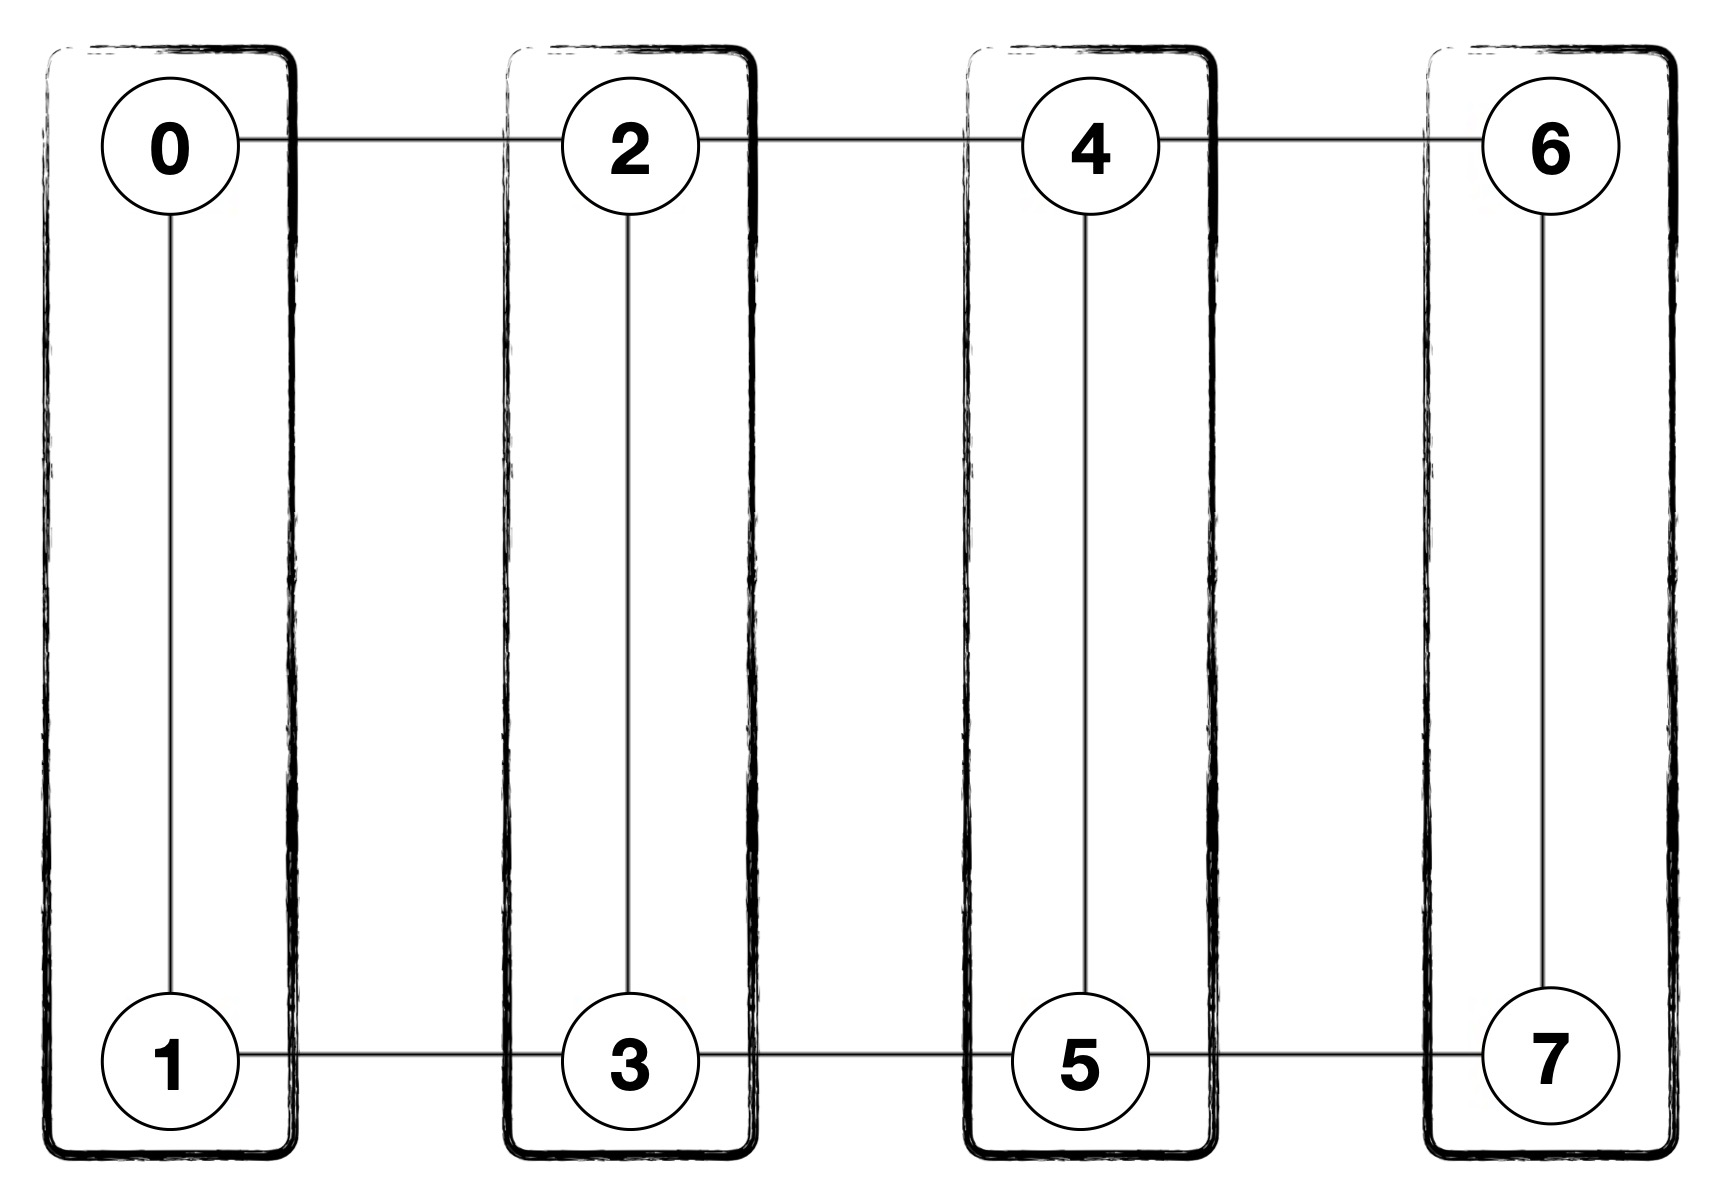
\includegraphics[scale=0.15]{grid.jpg}
    \caption{Graph of grid qubit-connectivity. Circled number represent qubits, black lines represent that two qubits are connected, and lack rectangles represent gates $A$.}
    \label{fig:grid}
\end{figure}
In the case of subspace QSCA, as long as $U$ can prepare $\ket{\phi^n_k}$ with linear-connectivity (reference \cite{ref:dicke_prep} and chapter \ref{chap:vpds}), then the algorithm itself only requires linear connectivity \ref{fig:linear_con}.

\section{Demonstration}

Here we given a demonstration of QCSA. We have developed code that performs QCSA: taking in an arbitrary quantum circuit and transforming it to the squeezed version of itself. We tested the algorithm using the following procedure: for various initial circuit depths ($n$), we estimated the density matrix ($\rho_{\text{est}}$) of the final state of each circuit (original and squeezed) using quantum state tomography (\ref{eq:simple_mat_els}) and compared its corresponding exact density matrix ($\rho_{\text{ext}}$) by taking the fidelity of the two. The definition of fidelity that we used can be defined as follows. Let $\rho$ and $\sigma$ be two density matrices, where the density matrix $\rho$ of a state $\ket{\phi}$ is defined as ($\rho = \ket{\psi}\bra{\psi}$).
Then their fidelity $F(\sigma,\rho)$ is defined as the trace of their product
\begin{align}
\label{def:fidelity}
\text{Tr}(\sigma\rho).
\end{align}
Quantum state tomography is the process by which the density matrix of a $n$-qubit state $\ket{\psi}$ is estimated as
\begin{align}
\label{quantum_state_tomo}
\rho=\frac{1}{2^n}\sum_{\alpha_1,\ldots,\alpha_n=0}^3S_{\alpha_1,\cdots,\alpha_n}\sigma^{(\alpha_0)}\otimes\ldots\otimes\sigma^{(\alpha_n)},
\end{align}
where  $\sigma^0=I$, $\sigma^1=X$, $\sigma^2=Y$, and $\sigma^3=Z$ are the Pauli operators and
\begin{align}
S_{\alpha_1,\ldots,\alpha_n}
=
\mel{\psi}{\sigma^{(\alpha_0)}\otimes\ldots\otimes\sigma^{(\alpha_n)}}{\psi},
\end{align}
are the expectation values of the Pauli-strings $sigma^{(\alpha_0)}\otimes\ldots\otimes\sigma^{(\alpha_n)}$ which are estimated using the method described in subsection \ref{expectation_values}. We studied the case with three initial qubits ($m_i=3$), a squeezing factor of $d=2$, and let the initial depth run over $n_i=2,3,\ldots,18$. The original circuits were populated with random three-qubit gates and each estimation of fidelity was averaged over five runs. The number of shots used for the squeezed circuit $s_f$ was $s_f=2^{m(d-1)}s_i=8s_i$ where $s_i=2^11$ is the number of shots used for the original circuit. The results were obtained from a noisy simulation of the quantum circuits on a classical computer. It can be seen in Figure \ref{fidelity_comp_graph} that the the fidelity estimated from the squeezed circuit is always greater than that estimated from the original circuit, the difference becoming more pronounced as the absolute difference in their depths grows with the increase in the original circuits depth $n_i$. As the squeezing factor was $d=2$, that means the ratio of the circuit depths $n_f/n_i$ approaches 2 as $n_i$ grows. Here, $n_f$ is the squeezed circuit depth.
\begin{figure}[H]
    \centering
    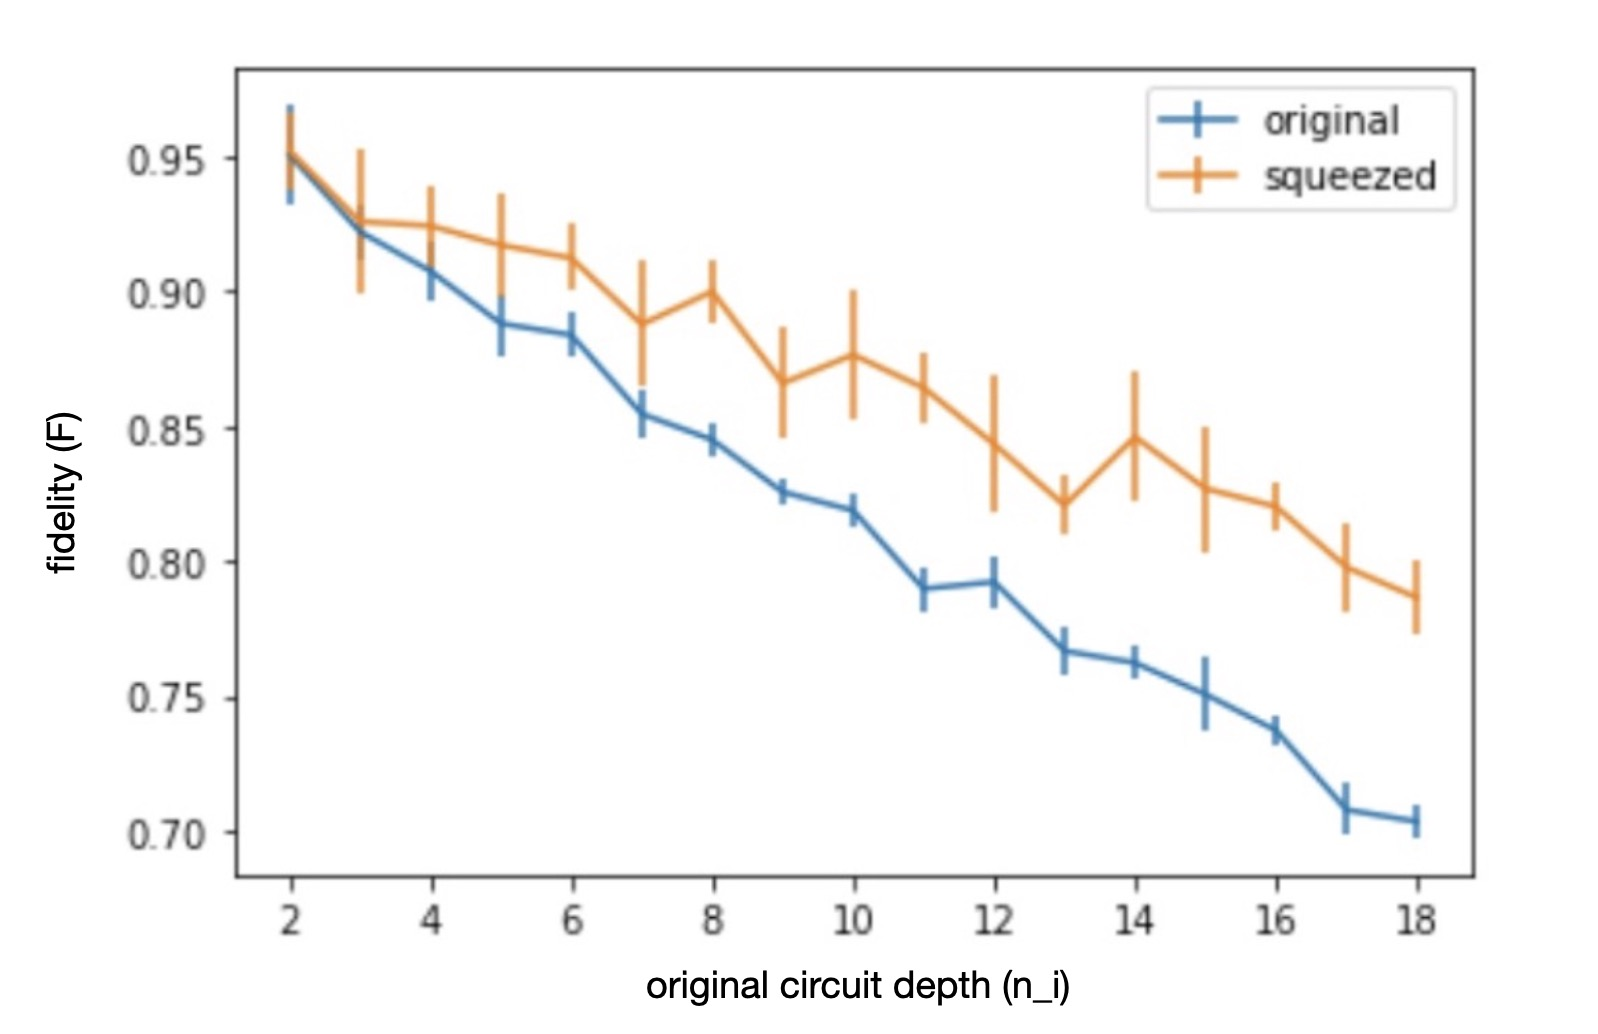
\includegraphics[scale=0.2]{fidelity_comp_graph.jpg}
    \caption{Comparison of fidelities of estimated and exact density matrices of both original and squeezed circuits.}
    \label{fidelity_comp_graph}
\end{figure}

\section{Conclusion}

In this chapter, we have presented the quantum circuit squeezing algorithm (QCSA), a novel quantum algorithm that trades more qubits and shots for a shorter circuit depth. To explain the algorithm, we first introduced the concepts of maximal entanglement, the ricochet property, and the entanglement swapping property. It was then shown how the entanglement property can be extended recursively. Additionally, a modification of QCSA to deal with Hamming weight preserving subspaces was introduced which ultimately improved the time scaling qubit connectivity requirements of the algorithm. It was then shown how all of these techniques could be combined to create QCSA. An analysis of the scaling of various complexities of the algorithm was conducted. Finally, we demonstrated the algorithm by running noisy simulations of it to show that the resulting squeezed circuits were less affected by the noise due to their shorter depth. As NISQ era devices require short depth circuits due to their high noise levels and are rapidly growing in their number of qubits, QCSA has the potential to be very beneficial in the near future by allowing researchers to run quantum circuits that otherwise would have been lost to the noise of our era's quantum machines.

\chapter{Variational Preparation of Dicke States}
\label{chap:vpds}

\section{Introduction}

Several chapters of this thesis involve the use of Dicke states. Chapter \ref{chap:lipkin_model} uses them to construct the ansatz for one mapping of the problem and again used Dicke states to map the problem to a smaller set of qubits. Additionally, chapter \ref{chap:pairing_model} used them as an initialization strategy for a novel type of ansatz to solve the model in an extreme case. Finally, chapter \ref{chap:qcsa} relied on the construction of them for a modification of the algorithm for Hamming weight preserving gates. Therefore, it is clear that an efficient algorithm to construct Dicke states would be very beneficial to many areas of the application of NISQ algorithms to many-body nuclear physics. While a deterministic method exists to do so that is linear in the number of qubits (\cite{ref:dicke_prep} and, \cite{ref:dicke_prep_dac}) the quantum circuit constructed is often still too long to be implemented on noisy quantum devices of the NISQ era. As an alternative we present here a short-depth, variational algorithm with the potential to prepare Dicke states with a shorter depth than the previously mentioned algorithm.

First, let us start with a few definitions. A Dicke state $\ket*{D^n_k}$ is the equal superposition of all $n$-qubit states $\ket{x}$ with Hamming weight $\text{wt}(x)=k$; that is
\begin{align}
\ket{D_k^n}={n \choose k}^{-\frac{1}{2}}
\sum_{\substack{x\in\{0,1\}^n\\ \textrm{wt}(x)=k}}\ket{x}.
\end{align}
For example,
\begin{align}
\ket{D^4_2}=\frac{1}{\sqrt{6}}
\left(
\ket{1100}+\ket{1010}+\ket{1001}+\ket{0110}+\ket{0101}+\ket{0011}.
\right)
\end{align}

A Dicke-like state $\ket{Dl^n_k(m)}$ is the equal superposition of $m$, $n$-qubit states $\ket{x}$ with Hamming weight $\text{wt}(x)=k$ up to possible relative phases of +1,
\begin{align}
\ket{Dl_k^n}={n \choose m}^{-\frac{1}{2}}
\sum_{\substack{x\in\{0,1\}^n\\ \textrm{wt}(x)=k}}(-1)^{f(x)}g(x)\ket{x}
,\end{align}
where $g(x)=0,1$ such that $g(x)=1$ only for $m$ states $x$. Thus a Dicke-like state is a phased Dicke state that's missing some bit-string states in its superposition. An example would be
\begin{align}
\ket{Dl^4_2(4)}=\frac{1}{\sqrt{6}}
\left(
\ket{1100}-\ket{1010}+\ket{1001}-\ket{0110}.
\right)
\end{align}
As discussed in the motivation section, we seek to find a quantum circuit that prepares the Dicke states with the shortest circuit depth possible. Here I propose a hybrid quantum-classical algorithm called the Variational State Preparation Algorithm (VSPA) to find such a circuit. VSPA is hybrid because it uses both a quantum and classical computer. The quantum computer's role is to implement a parameterized quantum circuit that tries to implement a Dicke state. Upon measurement of the quantum computer, a classical computer does post-measurement calculations to calculate a cost function which characterizes the overlap of the prepared state with the desired Dicke state. A classical optimization algorithm varies the parameters of the quantum circuit in order to minimize the cost function as much as possible. This results in the quantum circuit preparing a quantum state that has a desired overlap with the desired Dicke state. 

\section{The Algorithm}
The variational quantum circuit is parameterized by a set of parameters that are tuned by the classical optimization algorithm. The circuit consists of two parts: alternating $k$-state preparation and variational mixing. First, the quantum computer is put into an alternating $k$-state which is a particular quantum state with Hamming weight $k$. For $n$ qubits, the alternating $k$-state of type $t=\text{I, II, III}$, $\ket*{A^n_k}_{t}$ is the quantum state whose qubits alternate between 1 and 0 for the middle $2k$ qubits and are all 0 for the rest,
\begin{align}
\ket{A^n_k}_\text{I} &= \ket{...f(i)...} \ | \  \begin{cases}
f(i)= i+1 \ (\text{mod} \  2), & \left\lfloor\frac{n}{2}-1\right\rfloor - (k-1) \leq i \leq \left\lfloor\frac{n}{2}-1\right\rfloor + (k-1)
\\
f(i)= 0, & \text{otherwise}
\end{cases}
\\
\ket{A^n_k}_\text{II} &= \ket{...f(i)...} \ | \  \begin{cases}
f(i)= i \ (\text{mod} \  2), & \left\lfloor\frac{n}{2}-1\right\rfloor - (k-1) \leq i \leq \left\lfloor\frac{n}{2}-1\right\rfloor + (k-1)
\\
f(i)= 0, & \text{otherwise}
\end{cases}
\\
\ket{A^n_k}_\text{III} &= \frac{1}{\sqrt{2}}\left(\ket{A^n_k}_\text{I}+ \ket{A^n_k}_\text{II}\right)
,\end{align}
where $k=1,...,\lfloor k/2 \rfloor$.
For example
\begin{align}
\ket{A^6_2}_\text{I} &= \ket{010100},
\\
\ket{A^6_2}_\text{II} &= \ket{001010},
\\
\ket{A^6_2}_\text{III} &= \ket{0}\frac{\ket{1010}+\ket{0101}}{\sqrt{2}}\ket{0}
.\end{align}
To prepare $\ket*{A^n_k}_t$ for $k=\lfloor k/2 \rfloor+1,...,n$ one would finish by applying $X$ gates to all qubits since
\begin{align}
\ket{A^n_{n-k}}_t=X^{\otimes n}\ket{A^n_k}_t
.\end{align}
For $n$ qubits, the alternating $k$-state of type I (II) can be prepared on a quantum computer by applying an $X$ gates to all qubits that must be 1 (a quantum circuit of depth one). The alternating $k$-state of type III can be prepared with a circuit of depth $3$ with grid connectivity and depth $\mathcal{O}(n)$ with linear connectivity: Given a grid architecture, the $n$-qubit alternating $k$-state of type III can be implemented
with the following constant (2) depth circuit. For example, the circuit for $\ket{A^6_2}$ is shown below for six qubits:
\begin{align}
\Qcircuit @C=1em @R=1em { 
\lstick{\ket{0}} & \gate{H} & \ctrl{1} & \ctrl{2} & \qw & \qw & \qw & \qw
\\
\lstick{\ket{0}} & \gate{X} & \targ & \qw & \ctrl{2} & \qw & \qw & \qw
\\
\lstick{\ket{0}} & \qw & \qw & \targ & \qw & \ctrl{2} & \qw & \qw 
\\
\lstick{\ket{0}} & \qw & \qw & \qw & \targ & \qw & \ctrl{2} & \qw
\\
\lstick{\ket{0}} & \qw & \qw & \qw & \qw & \targ & \qw & \qw
\\
\lstick{\ket{0}} & \qw & \qw & \qw & \qw & \qw & \targ & \qw
}
\end{align}
The first two rows prepare the Bell state $\ket{\psi^+}=(\ket{01}+\ket{10})/\sqrt{2}$ and each subsequent pair of CNOTs ``copies" the state of each term of the Bell state and adds it onto that term. Given a linear nearest-neighbor (LNN) architecture
the $n$-qubit alternating $k$-state of type III can be implemented with the following $2n+1$ depth circuit. For example, the circuit for $\ket{A^6_2}$ is shown below for six qubits:
\begin{align}
\Qcircuit @C=1em @R=1em { 
\lstick{\ket{0}} & \gate{H} & \ctrl{1} & \qw & \ctrl{1} & \qw & \qw & \qw & \qw 
\\
\lstick{\ket{0}} & \gate{X} & \targ & \qswap & \targ & \qswap & \qw & \qw & \qw
\\
\lstick{\ket{0}} & \qw & \qw & \qswap\qwx & \ctrl{1} & \qswap\qwx & \ctrl{1} & \qw & \qw
\\
\lstick{\ket{0}} & \qw & \qw & \qw & \targ & \qswap & \targ & \qswap & \qw
\\
\lstick{\ket{0}} & \qw & \qw & \qw & \qw & \qswap\qwx & \ctrl{1} & \qswap\qwx & \qw
\\
\lstick{\ket{0}} & \qw & \qw & \qw & \qw & \qw & \targ & \qw & \qw
}
\end{align}

Once an alternating $k$-state has been prepared, the next step is to apply layers of parameterized, two-qubit, Hamming weight preserving gates called partial-SWAP gates. The partial-SWAP gate parameterized by $\theta$ is defined to be
\begin{align}
\text{pSWAP}(\theta)
=
e^{i\theta(XY-YX)/2}
=
\begin{pmatrix}
1 & 0 & 0 & 0 \\
0 & \cos\theta & -\sin\theta & 0 \\
0 & \sin\theta & \cos\theta & 0 \\
0 & 0 & 0 & 1
\end{pmatrix}
.\end{align}
Being in the group $SO(4)$, the pSWAP gate can be decomposed into a circuit of depth at most five, containing at most two CNOTs and twelve single-qubit rotations gates [4]. Note that pSWAP$(\theta)$ corresponds to a rotation in the subspace $\{\ket{01},\ket{10}$ by the angle $\theta$ (leaving the subspace $\{\ket{00},\ket{11}$ unchanged):
\begin{align}
\text{pSWAP}(\theta)\ket{00} &= \ket{00}
\\
\text{pSWAP}(\theta)\ket{01} &= \cos\theta\ket{01} + \sin\theta\ket{10} 
\\
\text{pSWAP}(\theta)\ket{10} &= \cos\theta\ket{10} - \sin\theta\ket{01} 
\\
\text{pSWAP}(\theta)\ket{11} &= \ket{11}
,\end{align}
thus preserving Hamming weight. Using pSWAP gates as mixing gates will always result in a Dicke-like state since there are no complex phases in their matrix representation (only a minus sign). A mixing layer is defined to be a single column of parameterized pSWAP gates being applied in parallel. The variational mixing part of the VSPA algorithm consists of several mixing layers. The first layer is applied to the middle $2k$ qubits. Each subsequent layer is applied to two additional qubits than the layer before - the qubit directly above and the qubit directly below the previous set of qubits (unless such qubit does not exist). The pseudo-code for the variational mixing part is given below:

\begin{algorithm}[H]

\caption{Variational Mixing Algorithm}\label{lphsn}

\hspace*{\algorithmicindent} \textbf{Input:} Number of qubits $n$, Hamming weight $k$, number of layers $l$, set of angles $\{\theta\}$.
\\
\hspace*{\algorithmicindent} \textbf{Output:} Quantum circuit implementation of variational mixing section of VSPA.

\begin{algorithmic}[H]

\State index$\_$list = [$\ $]

\State 

\State $i=\left\lfloor\frac{n}{2}-1\right\rfloor - (k-1)$
\While{$i \leq \left\lfloor\frac{n}{2}-1\right\rfloor + (k-1)$}
    \State index$\_$list.append(i)
    \State $i+=2$
\EndWhile

\State 

\State theta$\_$index $= 0$
\For{$0 \leq l \leq \text{layer}$}
    \If{$l\neq0$}
        new$\_$index$\_$list = [$\ $]
        \For{$i$ in index$\_$list}
            \State new$\_$index$\_$list.append($i-1$)
        \EndFor
        \State new$\_$index$\_$list.append($i+1$)
        \State index$\_$list=new$\_$index$\_$list
    \EndIf
    \For {$q$ in index$\_$list}
        \If{$0\leq q<n-1$}
            \State Append pSWAP($\theta$[theta$\_$index]) to qubits $q$ and $q+1$ of the quantum circuit
            \State theta$\_$index $+=1$
        \EndIf
    \EndFor
\EndFor

\end{algorithmic}

\end{algorithm}

\section{Calculating a Cost Function}

\hspace{5mm} As discussed above, our use of pSWAP gates as mixing gates will always result in a state that is the superposition of terms that all have the same Hamming weight. This should make it easier to minimize a cost function that measures the overlap of the variationally prepared state and a desired Dicke-like state. One good cost-function to quantify how close a variationally prepared state is to an $n$-qubit, $m$-term Dicke-like state $\ket{Dl^n_k(m)}$  would be:
\begin{align}
f_{\text{cost}}(\ket{\psi})=\text{Var}\{\abs{\bra{x}\ket{\psi}}^2 | x\in\{0,1\}^n | \text{wt}(x)=k \},
\end{align}     
That is, the variance of the list of probabilities of measuring every possible $\ket{x}$ with Hamming weight $k$. The variance makes a good cost function as it measures the deviations of a set from their average and the set of probabilities of an exact Dicke state would all be exactly zero, thus having a variance of zero. The closer the probabilities are to their average, the smaller the variance will be. These probabilities can be estimated by preparing and measuring the VSPA circuit multiple times and dividing the number of times one measured $\ket{x}$ by the total number of measurements made. The variance of the coefficients' absolute value squared is minimized when they are all equal (equal super-position) and is a measure of how close they are to being equal. Now, there are two variables to play with here that one may like to control: $g_n=1-\sum_xg(x)$ and $f_n=1-\sum_xf(x)$. Minimizing the first means maximizing the number of terms in the Dicke-like state, making the state a closer approximation to a true Dicke state. Minimizing the second means minimizing the number of terms that have a minus sign in front of them, again making the state a closer approximation to a true Dicke state. Another good candidate for a cost-function would be
\begin{align}
f_{\text{cost}}(\ket{\psi})=1-\frac{1}{|x(l')|}\left(\sum_{x\in x(l')}\sqrt{\abs{\bra{x}\ket{\psi}}^2}\right)^2
,\end{align}
where $l'\leq l$, which is one minus the square of the sum of the square roots of the probabilities. It is equal to one minus the overlap between our prepared state $\ket{\psi}$ and a desired non-phased Dicke-like state if one assumes no phases in the prepared state. Even if the prepared state does have phases, it should still serve as a good cost-function because it minimizes the difference between the absolute squares of the coefficients. Note that $f_n$ cannot be controlled using either of these cost function alone because using the probabilities (absolute values squared) of the coefficients erases all plus-or-minus phase information. However, it may be discovered that having plus-or-minus phased Dicke states is still beneficial in some circumstances such as in the multi-configuration method (subsection \ref{subsec:multi_conf} of chapter \ref{chap:pairing_model}) as the solution to the pairing model for large $g$ is not exactly a Dicke state but one close to it anyways.

\section{Results}

First, we created code to deterministically prepare Dicke states using the method given in \cite{ref:dicke_prep}. We have created code to run my novel VSPA algorithm using either of the first two cost-functions discussed above. We have used this algorithm to prepare Dicke state approximations to $\ket*{D^n_2}$ (where $n=4,5,6$) that each have a higher overlap with the true Dicke state than their deterministically (\cite{ref:dicke_prep}) prepared counterparts when simulated with noise (Figure \ref{fig:dicke_overlap}). This is because, as seen in Figure \ref{fig:dicke_comp}, while the deterministic preparation would in theory, create a perfect Dicke state, its depth is so much longer than our variational circuit that, when noise is included, creates a worse approximation to the true Dicke state. The idea is that, even though the variational method may not be able to exactly prepare an exact Dicke state (which would require exactly minimizing the cost function in a noisy environment), it has the potential to get closer than the deterministic method once one accounts for the extra noise that befalls the latter. In the bottom half of Figure \ref{fig:dicke_comp}, we have a histogram of the measurements obtained through noisy simulation. The measurements that have a Hamming weight of two (the only ones which should have been measured) are highlighted in red. All non-feasible (with a Hamming weight other than two) are highlighted in blue. With this, it can clearly be seen that in this case, the variational method is much less affected by noise as the non-feasible states are measured with much less frequency than in the deterministic method. Next, the number of CNOTs is noted to be significantly less for the variational method, likely due to the large number of the three-qubit, double controlled gates that had to be decomposed into several CNOTs each for the deterministic method. This was also a likely factor in improving the results as the CNOT is noisier than the single-qubit gates. Finally, we note the high number of CNOTs in the the deterministic method circuit which connect non-neighboring qubits. As we simulated the results on a noisy model that assumed only linear connectivity of qubits, the compiler for the deterministic method's circuit had to add several more swap gates (which require 3 CNOTs) compared to the variational method's in order to move the non-neighboring qubits next to one another. This is because the deterministic method's circuit has six non-neighboring CNOTs, compared to the variational method's two. 

\begin{figure}
    \centering
    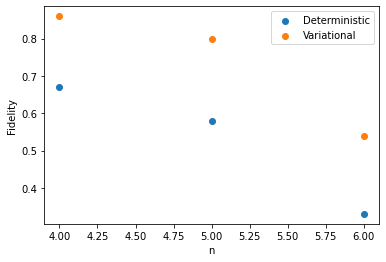
\includegraphics[scale=0.6]{d_vs_v.png}
    \caption{Overlap of Deterministically vs Variationally prepared Dicke-states with true Dicke-state}
    \label{fig:dicke_overlap}
\end{figure}

\begin{figure}
    \centering
    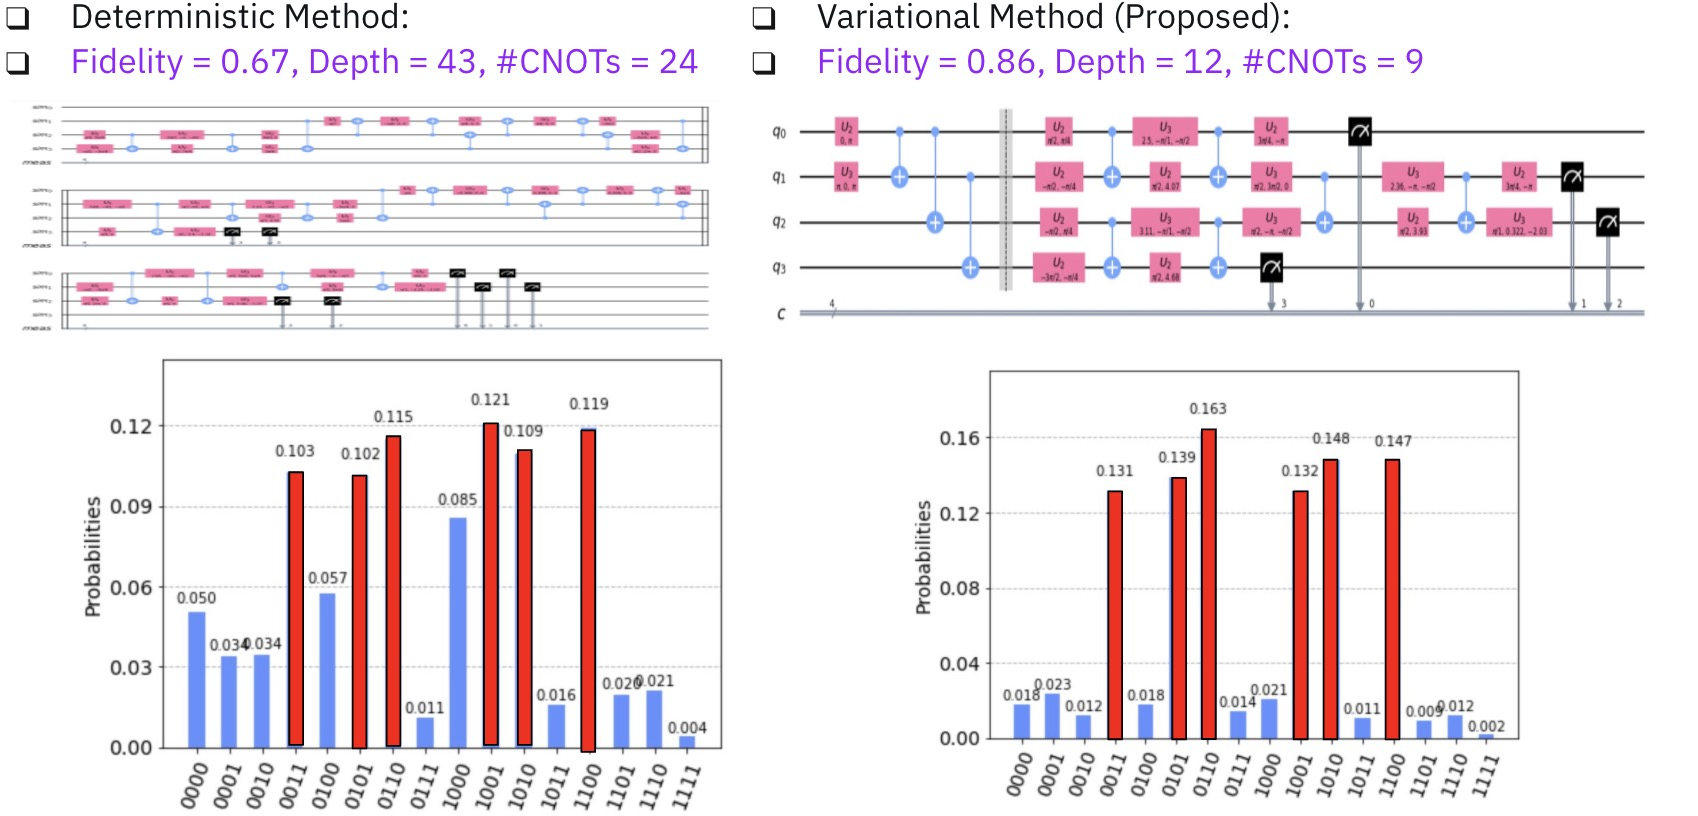
\includegraphics[scale=0.3]{d42.jpg}
    \caption{Comparison of Deterministic and Variational Methods to prepare the Dicke state $\ket*{D^4_2}$}
    \label{fig:dicke_comp}
\end{figure}

\section{Conclusion}

In this section, we developed the variational Dicke state preparation algorithm (VSPD), a novel variational algorithm to prepare Dicke and Dicke-like states. We laid forth a short-depth variational ansatz which can efficiently search the appropriate Hamming weight restricted subspace. We also discussed different cost functions which could be used for the minimization subroutine. Finally, we presented results obtained from testing the algorithm with noisy simulations and bench-marked them favorably against a previously developed deterministic method \cite{dick_prep}. In the future, one might wish to compare and contrast different ansatz and cost functions to prepare Dicke state $\ket*{D^n_k}$ for even more values of $n$ and $k$. Additionally, one could look into determining a way to fix the phases $f(x)$ of the terms of the variational Dicke state prepared. One potential way to do this would simply to have the ansatz and cost-function be identical to that introduced for the pairing model in chapter \ref{chap:pairing_model}) with the pairing strength $g$ set to zero. This is because, as proven in subsection \ref{subsec:multi_conf}, the Dicke states are the eigenstates of said model. We conclude this section by reiterating the widespread potential use of Dicke states: both as part of ansatz construction for many-body nuclear physics models like the Lipkin and pairing model, and as part of entangling process of the subspace QCSA algorithm from the previous section.

\chapter{Conclusion}

In this thesis, we have provided the basis for which future quantum algorithms can be developed to solve many-body nuclear problems. For the Lipkin model, we developed techniques to make the ansatz for different mappings of the problem lower-depth. We also developed a mapping that cut the number of required qubits in half. For the pairing model, we estimated the ground state energy with the variational quantum eigensolver (VQE) and bench-marked the results against the classical algorithm pair coupled cluster theory (pCCD). We also developed techniques to reduce the circuit depth for the unitary pair coupled cluster doubles (UpCCD) ansatz for quantum computers with circular connectivity that has a lower depth than the ansatz for devices with linear connectivity (\ref{fig:linear_con}). We also developed an algorithm for finding the energies of excited states for the model. Finally, we developed a novel ansatz in which one starts the quantum computer in a Dicke state in order to solve the pairing model for large values of the pairing strength $g$. In the collective neutrino oscillations chapter, we presented the first digital simulation of the model on a real quantum computer. We used this to study the time-evolution and entanglement of the system. We applied error mitigation techniques to improve the accuracy of our results. Then we presented the quantum circuit squeezing algorithm and showed how it could be used to reduce the circuit depth and therefore improve the results of arbitrary quantum circuits. Finally, we presented our novel algorithm to variationally prepared Dicke states.

As this work was meant to serve as a springboard of which future developments in the field could be accomplished, we discuss here several future extensions and applications of this work. For the Lipkin model, one could explicitly compare the different mappings and ansatzes discussed to have better evidence that the one we choose to pursue is truly the best choice. One could do this by running tests on the gradients of the wave-function to see if either of the methods lends itself more easily to the problem of the barren plateau (exponentially vanishing gradients). In terms of the pairing model, one would desire to compare our iterative quantum excited states algorithm to other algorithms that attempt to accomplish the same thing. Additionally, one would like to run the VQE algorithms of this section on the quantum computers of the near future (via the cloud) that would allow the frequent calls to the quantum computer that is required for VQE. As for the collective neutrino oscillation simulations, one would like to compare various permutations of the Trotter terms that make up the ansatz to see if putting the terms with the highest commutator with the Hamiltonian first would improve the results on an actual quantum computer. The reasoning behind this is that, because the qubits decohere exponentially, putting the most important terms of the ansatz first would give said terms the least noisy effect on the quantum state. For the quantum circuit squeezing algorithm, one could apply it to a pre-existing algorithm like VQE to see if it improves the accuracy of the results. Finally, the variational preparation of Dicke states could similarly be applied to pre-existing algorithms that would benefit from the initialization of their circuits into a Dicke state. In the far future, one would like to see the improved quantum computers of that time be used to tackle the problems of nuclear physics that are too complex for today's classical computers, serving as a light in the long tunnel of our ignorance towards the hidden treasures buried deep below.

% appendices
\begin{appendices}

\chapter{Angular Momentum Commutation Relations} 
\label{appendix:angular_momentum_commutation_relations}

In this appendix we prove the mapping between the angular momentum SU(2) operators ($J_+$, $J_-$, and $J_z$) and the fermionic creation and annihilation operators ($a$ and $a^\dagger$). The mappings (\ref{jz}) and (\ref{jpm}) are shown to hold through the demonstration that the SU(2) commutation relations (\ref{comm1}) and (\ref{comm2}) hold under the substitution of fermionic operators for SU(2) operators from the mappings. Here we define $j_{m\pm}= a^\dagger_{m\pm}a_{m\mp}$. We have that
\begin{align}
\comm*{J_+}{J_-}
&=
\comm*{\sum_mj_{m+}}{\sum_nj_{n-}}
\nonumber
\\
&=
\sum_{mn}\comm*{j_{m+}}{a^{\dagger}_{n-}a_{n+}}
\nonumber
\\
&=
\sum_{mn}\left(\comm*{j_{m+}}{a^{\dagger}_{n-}}a_{n+}+a^{\dagger}_{n-}\comm*{j_{m+}}{a_{n+}}\right)
\nonumber
\\
&=
\sum_{mn}\delta_{mn}\left(a^{\dagger}_{m+}a_{n+}-a^{\dagger}_{n-}a_{m-}\right)
\nonumber
\\
&=
\sum_{m}\left(a^{\dagger}_{m+}a_{m+}-a^{\dagger}_{m-}a_{m-}\right)
\nonumber
\\
&=2J_z,
\end{align}
and
\begin{align}
\comm*{J_z}{J_\pm}
&=
\comm*{\frac{1}{2}\sum_{m\sigma}\sigma a^{\dagger}_{m\sigma}a_{m\sigma}}{\sum_{n}j_{n\pm}}
\nonumber
\\
&=
\frac{1}{2}\sum_{mn\sigma}\sigma\comm*{a^{\dagger}_{m\sigma}a_{m\sigma}}{j_{n\pm}}
\nonumber
\\
&=
\frac{1}{2}\sum_{mn\sigma}\sigma
\left(
a^{\dagger}_{m\sigma}\comm*{a_{m\sigma}}{j_{n\pm}}
+
\comm*{a^{\dagger}_{m\sigma}}{j_{n\pm}}a_{m\sigma}
\right)
\nonumber
\\
&=
\frac{1}{2}\sum_{mn\sigma}\sigma
\left(
\delta_{\sigma\pm}a^{\dagger}_{m\sigma}a_{n\mp}
-
\delta_{-\sigma\pm}a^{\dagger}_{n\pm}a_{m\sigma}\right)
\nonumber
\\
&=
\pm\sum_ma^{\dagger}_{m\pm}a_{m\mp}
\nonumber
\\
&=
\pm J_{\pm},
\end{align}
where we've used the commutations of the SU(2) ladder operator and the fermionic operators which are derived below
\begin{align}
\label{kad}
\comm{j_{p\sigma}}{a^{\dagger}_{q\tau}}
&=
\comm{a^{\dagger}_{p\sigma}a_{p-\sigma}}{a^{\dagger}_{q\tau}}
\nonumber
\\
&=
a^{\dagger}_{p\sigma}\comm{a_{p-\sigma}}{a^{\dagger}_{q\tau}}
+
\comm{a^{\dagger}_{p\sigma}}{a^{\dagger}_{q\tau}}a_{ p-\sigma}
\nonumber
\\
&=
a^{\dagger}_{p\sigma}\left(\acomm{a_{p-\sigma}}{a^{\dagger}_{q\tau}}-2a^{\dagger}_{q\tau}a_{p-\sigma}\right)
\nonumber
\\
&+
\left(\acomm{a^{\dagger}_{p\sigma}}{a^{\dagger}_{q\tau}}-2a^{\dagger}_{q\tau}a^{\dagger}_{p\sigma}\right)a_{p-\sigma}
\nonumber
\\
&=
\delta_{pq}\delta_{-\sigma\tau}a^{\dagger}_{p\sigma}-2\acomm{a^{\dagger}_{p\sigma}}{a^{\dagger}_{q\tau}}a_{p-\sigma}
\nonumber
\\
&=
\delta_{pq}\delta_{-\sigma\tau}a^{\dagger}_{p\sigma}
\end{align}
\begin{align}
\label{ka}
\comm{j_{p\sigma}}{a_{q\tau}}
\nonumber
&=
-\comm{a_{q\tau}}{k_{p\sigma}}
\nonumber
=
-\comm{k_{p\sigma}^{\dagger}}{a^{\dagger}_{q\tau}}^{\dagger}
\nonumber
\\
&=
-\comm{k_{p-\sigma}}{a^{\dagger}_{q\tau}}^{\dagger}
\nonumber
=
-(\delta_{pq}\delta_{\sigma\tau}a^{\dagger}_{p-\sigma})^{\dagger}
\nonumber
\\
&=
-\delta_{pq}\delta_{\sigma\tau}a_{p-\sigma}
.\end{align}

\chapter{Normalization of the Hartree-Fock Ansatz}
\label{appendix:normalization_of_the_hartree-fock_ansatz}

In this appendix we derive the normalization of the Hartree-Fock ansatz.
The definition of a coherent state, applied to the group SU(2), gives that the SU(2) coherent state takes the form
\begin{align}
\ket{\tau}=e^{\zeta J_+-\bar{\zeta}J_-}\ket{0},
\end{align}
where $\xi=(\theta/2)e^{-i\phi}$. We wish to write the coherent state in the form
\begin{align}
\ket{\tau}'=Ne^{\tau J_+}\ket{0},
\end{align}
which we will do through the use of the SU(2) generating function
\begin{align}
\label{gf}
&\bra{\tau}e^{\tau}e^{\alpha_0J_0}e^{\alpha_-J_-}\ket{\tau}
\\
= \ &
(1+\abs{\tau}^2)^{-2J}\left[e^{\alpha_0/2}\abs{\tau}^2+e^{-\alpha_0/2}(\alpha_+\tau^*+1)(\alpha_-\tau+1)\right]^{2J},
\end{align}
and the BCH equation
\begin{align}
e^{\zeta J_+-\bar{\zeta}J_-}
=
e^{\tau J_+}e^{\text{ln}(1+\abs{\tau}^2)J_0}e^{-\bar{\tau}J_-}.
\end{align}
If the two forms of the coherent state are equal, then
\begin{align}
&1
\\
= \ &\bra{\tau}\ket{\tau}^{'}
\\
= \ &
N\bra{\tau}e^{\tau J_+}\ket{0}
\\
= \ &
N\bra{\tau}e^{\tau J_+}e^{-(\zeta J_+-\bar{\zeta}J_-)}\ket{\tau}
\\
= \ &
N\bra{\tau}e^{\text{ln}(1+\abs{\tau}^2)J_0}e^{\bar{\tau}J_-}\ket{\tau}
\\
= \ &
(1+\abs{\tau}^2)^{-2J}\left[e^{\text{ln}(1+\abs{\tau}^2)/2}\abs{\tau}^2+e^{-\text{ln}(1+\abs{\tau}^2)/2}(1+\abs{\tau}^2)\right]^{2J}
\\
= \ &
(1+\abs{\tau}^2)^{-2J}\left[(1+\abs{\tau}^2)^{\frac{1}{2}}\abs{\tau}^2+(1+\abs{\tau}^2)^{-\frac{1}{2}}(1+\abs{\tau}^2)\right]^{2J}
\\
= \ &
(1+\abs{\tau}^2)^J,
\end{align}
which implies that $N=(1+\abs{\tau}^2)^{-J}$.

\chapter{Lipkin Hamiltonian for Hartree-Fock}
\label{appendix:lipkin_hamiltonian_matrix_elements_for_hf}

In this appendix, we derive the matrix element $\mel{\tau}{H}{\sigma}$ where $H$ is the Lipkin Hamiltonian and
\begin{align}
\ket{\tau}&=(1+\abs{\tau}^2)^{-\frac{\Omega}{2}}e^{\tau J_+}\ket{0},
\\
\ket{\sigma}&=(1+\abs{\sigma}^2)^{-\frac{\Omega}{2}}e^{\sigma J_+}\ket{0}
,\end{align}
are two arbitrary $SU(2)$ coherent states. Here $\ket{0}=\ket{J-J}$, $\tau=\tan(\theta/2)e^{-i\phi}$, $\sigma=\tan(\theta'/2)e^{-i\phi'}$, and $\Omega=J/2$. Expanding
\begin{align}
&\bra{\tau}H\ket{\sigma}
\\
= \ &
(1+\abs{\sigma})^{-\frac{\Omega}{2}}\bra{\tau}He^{\sigma J_+}\ket{0}
\\
= \ &
(1+\abs{\tau})^{\frac{\Omega}{2}}(1+\abs{\sigma})^{-\frac{\Omega}{2}}\bra{\tau}He^{(\sigma-\tau) J_+}\ket{\tau}
\\
= \ &
(1+\abs{\tau})^{\frac{\Omega}{2}}(1+\abs{\sigma})^{-\frac{\Omega}{2}}
\\
\times \ &
\left[\epsilon\bra{\tau}J_0e^{(\sigma-\tau) J_+}\ket{\tau}-\frac{1}{2}V\bra{\tau}(J^2_++J^2_-)e^{(\sigma-\tau) J_+}\ket{\tau}\right].
\end{align}
Using the SU(2) generating function
\begin{align}
&\bra{\tau}e^{\alpha_-J_-}e^{\alpha_0J_0}e^{\alpha_+J_+}\ket{\tau}
\\
= \ &
(1+\abs{\tau}^2)^{-\Omega}\left[e^{-\alpha_0/2}+e^{\alpha_0/2}(\bar{\tau}+\alpha_-)(\tau+\alpha_+)\right]^{\Omega},
\end{align}
we calculate each term separately, starting with
\begin{align}
&\bra{\tau}J_0e^{(\sigma-\tau) J_+}\ket{\sigma}
\nonumber
\\
= \ &
\frac{\partial}{\partial\alpha_0}\bra{\tau}e^{\alpha_0J_0}e^{(\sigma-\tau) J_+}\ket{\tau}\bigg{|}_{\alpha_0=0}
\nonumber
\\
= \ &
\frac{1}{(1+\abs{\tau}^2)^{\Omega}}\frac{\partial}{\partial\alpha_0}\left[e^{-\alpha_0/2}+\bar{\tau}\sigma e^{\alpha_0/2}\right]^{\Omega}\bigg{|}_{\alpha_0=0}
\nonumber
\\
= \ &
\frac{\Omega/2}{(1+\abs{\tau}^2)^{\Omega}}(\sigma\bar{\tau}e^{\alpha_0/2}-e^{-\alpha_0/2})(\sigma\bar{\tau}e^{\alpha_0/2}+e^{-\alpha_0/2})^{\Omega-1}\Bigg{|}_{\alpha_0=0}
\nonumber
\\
= \ &
\frac{\Omega/2}{(1+\abs{\tau}^2)^{\Omega}}(\sigma\bar{\tau}-1)(\sigma\bar{\tau}+1)^{\Omega-1},
\end{align}
followed by
\begin{align}
\\
&\bra{\tau}J^2_+e^{(\sigma-\tau) J_+}\ket{\sigma}
\nonumber
\\
= \ &
\frac{\partial^2}{\partial\alpha^2_+}\bra{\tau}e^{(\alpha_++\sigma-\tau) J_+}\ket{\tau}\bigg{|}_{\alpha_+=0}
\nonumber
\\
= \ &
\frac{1}{(1+\abs{\tau}^2)^{\Omega}}\frac{\partial^2}{\partial\alpha^2_+}\left[1+\bar{\tau}(\alpha_++\sigma)\right]^{\Omega}\bigg{|}_{\alpha_+=0}
\nonumber
\\
= \ &
\frac{\Omega(\Omega-1)}{(1+\abs{\tau}^2)^{\Omega}}(\bar{\tau}^2)[1+\bar{\tau}(\alpha_++\sigma)]^{\Omega-2}\bigg{|}_{\alpha_+=0}
\nonumber
\\
= \ &
\frac{\Omega(\Omega-1)}{(1+\abs{\tau}^2)^{\Omega}}(\bar{\tau}^2)(1+\bar{\tau}\sigma)^{\Omega-2},
\end{align}
followed by
\begin{align}
&\bra{\tau}J^2_-e^{(\sigma-\tau) J_+}\ket{\sigma}
\nonumber
\\
= \ &
\frac{\partial^2}{\partial\alpha^2_-}\bra{\tau}e^{\alpha_-J_-}e^{(\sigma-\tau) J_+}\ket{\tau}\bigg{|}_{\alpha_-=0}
\nonumber
\\
= \ &
\frac{1}{(1+\abs{\tau}^2)^{\Omega}}\frac{\partial^2}{\partial\alpha^2_-}\left[1+(\bar{\tau}+\alpha_-)\sigma\right]^{\Omega}\bigg{|}_{\alpha_-=0}
\nonumber
\\
= \ &
\frac{\Omega(\Omega-1)}{(1+\abs{\tau}^2)^{\Omega}}(\sigma^2)[1+(\bar{\tau}+\alpha_-)\sigma]^{\Omega-2}\bigg{|}_{\alpha_-=0}
\nonumber
\\
= \ &
\frac{\Omega(\Omega-1)}{(1+\abs{\tau}^2)^{\Omega}}(\sigma^2)(1+\bar{\tau}\sigma)^{\Omega-2}.
\end{align}
Combining yields
\begin{align}
\label{ths}
&\bra{\tau}H\ket{\sigma}
=
(\Omega/2)[(1+\abs{\tau}^2)(1+\abs{\sigma}^2)]^{-\frac{\Omega}{2}}
\nonumber
\\
\times \ &\left[ 
\epsilon(\sigma\bar{\tau}-1)(\sigma\bar{\tau}+1)^{\Omega-1}-V(\Omega-1)\left(\bar{\tau}^2+\sigma^2\right)(1+\bar{\tau}\sigma)^{\Omega-2}
\right].
\end{align}

\chapter{Dicke State Lemmas}
\label{app:dicke_state_lemmas}

In this appendix, we inductively prove the following two lemmas involving Dicke states
\begin{align}
\label{dsl1}
\sum_{p=1}^{n}A^\dagger_p\ket{D^n_k}
&=\sqrt{(n-k)(k+1)}\ket{D^n_{k+1}},
\\
\label{dsl2}
\sum_{p=1}^nA\ket{D^n_k}
&=\sqrt{(n-k+1)(k)}\ket{D^n_{k-1}},
\end{align}
The base case for the first lemma (\ref{dsl1}) is given by the case $(n,k)=(1,0)$ below
\begin{align}
\label{bc1}
A^\dagger_1\ket{D^1_0}
&=
A^\dagger_1\ket{0_1}
\nonumber
\\
&=
\ket{1_1}
\nonumber
\\
&=\ket{D^1_1}
\nonumber
\\
&=\sqrt{(1-0)(0+1)}\ket{D^1_1}.
\end{align}
Similarly, the base case for the second lemma (\ref{dsl2}) is given by the case $(n,k)=(1,1)$ below
\begin{align}
\label{bc2}
A_1\ket{D^1_1}
&=
A_1\ket{1_1}
\nonumber
\\
&=
\ket{0_1}
\nonumber
\\
&=\ket{D^1_0}
\nonumber
\\
&=\sqrt{(1-1+1)(1)}\ket{D^1_1}.
\end{align}
We prove the first lemma first by assuming, as our induction hypothesis, that (\ref{dsl1}) is true and show that it still holds when we take $n\to n+1$, as follows
\begin{align}
\sum_{p=1}^{n+1}A^\dagger_p\ket{D^{n+1}_k}
&=
\left(\sum_{p=1}^{n}A^\dagger_p + A^\dagger_{n+1}\right)\left(\sqrt{\frac{k}{n+1}}\ket{D^{n}_{k-1}}\ket{1}+\sqrt{\frac{n-k+1}{n+1}}\ket{D^{n}_k}\ket{0}\right),
\end{align}
where we took out the $n+1$ term from the sum and used the recursive definition of the Dicke state (\ref{dicke_def}).
Using the first base case (\ref{bc1}) yields
\begin{align}
\left(\sum_{p=1}^{n}A^\dagger_p\right)\left(\sqrt{\frac{k}{n+1}}\ket{D^{n}_{k-1}}\ket{1}+\sqrt{\frac{n-k+1}{n+1}}\ket{D^{n}_k}\ket{0}\right)
+
\sqrt{\frac{n-k+1}{n+1}}\ket{D^{n}_k}\ket{1}.
\end{align}
Applying the induction hypothesis (\ref{dsl1}) and then combining the first and last terms yields 
\begin{align}
&
(k+1)\sqrt{\frac{n-k+1}{n+1}}\ket{D^{n}_{k-1}}\ket{1}+\sqrt{(n-k)(k+1)}\sqrt{\frac{n-k+1}{n+1}}\ket{D^{n}_k}\ket{0}
\\
= \ &
\sqrt{(n-k+1)(k+1)}
\left(
\sqrt{\frac{k+1}{n+1}}\ket{D^{n}_{k-1}}\ket{1}+\sqrt{\frac{n-k}{n+1}}\ket{D^{n}_k}\ket{0}
\right)
\\
= \ &
\sqrt{(n-k+1)(k+1)}\ket{D^{n+1}_{k+1}},
\end{align}
which completes the proof. 

We now prove the second lemma first by assuming, as our induction hypothesis, that (\ref{dsl2}) is true and show that it still holds when we take $n\to n+1$, as follows
\begin{align}
\sum_{p=1}^{n+1}A_p\ket{D^{n+1}_k}
&=
\left(\sum_{p=1}^{n}A_p + A_{n+1}\right)\left(\sqrt{\frac{k}{n+1}}\ket{D^{n}_{k-1}}\ket{1}+\sqrt{\frac{n-k+1}{n+1}}\ket{D^{n}_k}\ket{0}\right),
\end{align}
where we took out the $n+1$ term from the sum and used the recursive definition of the Dicke state (\ref{dicke_def}).
Using the second base case (\ref{bc2}) yields
\begin{align}
\left(\sum_{p=1}^{n}A_p\right)\left(\sqrt{\frac{k}{n+1}}\ket{D^{n}_{k-1}}\ket{1}+\sqrt{\frac{n-k+1}{n+1}}\ket{D^{n}_k}\ket{0}\right)
+
\sqrt{\frac{k}{n+1}}\ket{D^{n}_{k-1}}\ket{0}
\end{align}
Applying the induction hypothesis (\ref{dsl2}) and then combining the first and last terms yields 
\begin{align}
&
\sqrt{(n-k+2)(k)}\sqrt{\frac{k-1}{n+1}}\ket{D^{n}_{k-2}}\ket{1}
+
(n-k+2)\sqrt{\frac{k}{n+1}}\ket{D^{n}_{k-1}}\ket{0}
\\
= \ &
\sqrt{(n-k+2)(k)}
\left(
\sqrt{\frac{k-1}{n+1}}
\ket{D^{n}_{k-2}}
\ket{1}
+
\sqrt{\frac{n-k+2}{n+1}}
\ket{D^{n}_{k-1}}
\ket{0}
\right)
\\
= \ &
\sqrt{(n-k+2)(k)}\ket{D^{n+1}_{k-1}},
\end{align}
which completes the proof.

\chapter{State-Overlap Algorithm}
\label{appendix:state_overlap_algorithm}

In this appendix we explain the efficient state-overlap algorithm that is used to find the eigen energies of excited states. Consider two states $\ket{\psi}=a\ket{0}+b\ket{1}$ and $\ket{\phi}=c\ket{0}+d\ket{1}$. The overlap between these two states is
\begin{align}
\abs{\bra{\psi}\ket{\phi}}^2
&=\left(a^*c+b^*d\right)\left(ac^*+bd^*\right)
\\
&=\abs{a}^2\abs{c}^2+\abs{b}^2\abs{d}^2+a^*bcd^*+ab^*c^*d.
\end{align}
Now consider the circuit
\begin{align}
\Qcircuit{
\lstick{\ket{\psi}} & \ctrl{1} & \gate{H} & \meter \\
\lstick{\ket{\phi}} & \targ & \qw & \meter
}
\end{align}
The progression of the state through the above circuit is
\begin{align}
\ket{\psi\phi}
&=ac\ket{00}+ad\ket{01}+bc\ket{10}+bd\ket{11} \\
&\to ac\ket{00}+ad\ket{01}+bc\ket{11}+bd\ket{10} \\
&\to \frac{1}{\sqrt{2}}\big[(ac+bd)\ket{00}+(ad+bc)\ket{01} \\
&+(ac-bd)\ket{10}+(ad-bc)\ket{11}\big].
\end{align}
The probability that $\ket{\psi\phi}=\ket{11}$ is
\begin{align}
P_{11}
&=\frac{1}{2}(ad-bc)(ad-bc)^* \\
&=\frac{1}{2}\left[|a|^2|d|^2+|b|^2|c|^2-ab^*c^*d-a^*bcd^*\right].
\end{align}
Note that
\begin{align}
&P_{00}+P_{01}+P_{10}-P_{11} \\
=&1-2P_{11} \\
=&1-\left[|a|^2|d|^2+|b|^2|c|^2-ab^*c^*d-a^*bcd^*\right] \\
=&|a|^2|c|^2+|b|^2|d|^2+ab^*c^*d+a^*bcd^* \\
=&\abs{\bra{\psi}\ket{\phi}}^2,
\end{align}
where we've used the fact that $1=|a|^2+|b|^2$. This can be generalized to
\begin{align}
\Qcircuit{
& \qw & \ctrl{4} & \qw &  \gate{\cdots} & \qw & \gate{H} & \meter \\ 
\lstick{\raisebox{-3.1em}{$\ket{\psi}$\ }} & \qw  & \qw & \ctrl{4} & \gate{\cdots} & \qw & \gate{H} & \meter \gategroup{1}{1}{4}{2}{.7em}{\{} \\
& \vdots & & & & & \vdots \\
& \qw  & \qw & \qw & \gate{\cdots} & \ctrl{4} & \gate{H} & \meter \\
& \qw & \targ & \qw & \gate{\cdots} & \qw & \qw & \meter \\
\lstick{\raisebox{-3.1em}{$\ket{\phi}$\ }} & \qw & \qw & \targ & \gate{\cdots} & \qw & \qw & \meter \gategroup{5}{1}{8}{2}{.7em}{\{}\\
& \vdots & & & & & \vdots & \\
& \qw & \qw & \qw & \gate{\cdots} & \targ & \qw & \meter
},
\end{align}
as explained in \cite{swap_test}.


\chapter{Pair Commutation Relations}
\label{appendix:pair_commutation_relations}

In this appendix, we use the fermionic anti-commutation relations (\ref{fermionic_anticommutation_relations})
to prove the pair fermionic commutation relations (\ref{AAd_comm}-\ref{NA_comm}).
The first commutation relation is proved as follows
\begin{align}
\comm*{A_p}{A^\dagger_q}
&=
\comm*{a_{p-}a_{p+}}{a^\dagger_{q+}a^\dagger_{q-}}
\\
&=
a_{p-}a^\dagger_{q+}\comm*{a_{p+}}{a^\dagger_{q-}}
+
a_{p-}\comm*{a_{p+}}{a^\dagger_{q+}}a^\dagger_{q-}
\nonumber
\\
&+
a^\dagger_{q+}\comm*{a_{p-}}{a^\dagger_{q-}}a_{p+}
+
\comm*{a_{p-}}{a^\dagger_{q+}}a^\dagger_{q-}a_{p+}
\\
&=
a_{p-}a^\dagger_{q+}\cancel{\acomm*{a_{p+}}{a^\dagger_{q-}}}
-
2a_{p-}a^\dagger_{q+}a^\dagger_{q-}a_{p+}
\nonumber
\\
&+
a_{p-}\acomm*{a_{p+}}{a^\dagger_{q+}}a^\dagger_{q-}
-
2a_{p-}a^\dagger_{q+}a_{p+}a^\dagger_{q-}
\nonumber
\\
&+
a^\dagger_{q+}\acomm*{a_{p-}}{a^\dagger_{q-}}a_{p+}
-
2a^\dagger_{q+}a^\dagger_{q-}a_{p-}a_{p+}
\nonumber
\\
&+
\cancel{\acomm*{a_{p-}}{a^\dagger_{q+}}}a^\dagger_{q-}a_{p+}
-
2a^\dagger_{q+}a_{p-}a^\dagger_{q-}a_{p+}
\\
&=
\delta_{pq}(a_{p-}a^\dagger_{q-}+a^\dagger_{q+}a_{p+})
\nonumber
\\
&-
2a_{p-}a^\dagger_{q+}\cancel{\acomm*{a^\dagger_{q-}}{a_{p+}}}
-
2a^\dagger_{q+}\acomm*{a^\dagger_{q-}}{a_{p-}}a_{p+}
\\
&=
\delta_{pq}(a_{p-}a^\dagger_{q-}-a^\dagger_{q+}a_{p+})
\\
&=
\begin{cases}
a_{p-}a^\dagger_{p-}-a^\dagger_{p+}a_{p+} & \text{if} \ p=q
\\
0 & \text{if} \ p\neq q
\end{cases},
\end{align}
which we now compare to
\begin{align}
\delta_{pq}(1-N_p)
&=
\delta_{pq}(\delta_{p-p-}-a^\dagger_{p+}a_{p+}-a^\dagger_{p-}a_{p-})
\\
&=
\delta_{pq}(a^\dagger_{p-}a_{p-}+a_{p-}a^\dagger_{p-}-a^\dagger_{p+}a_{p+}-a^\dagger_{p-}a_{p-})
\\
&=
\delta_{pq}(a_{p-}a^\dagger_{p-}-a^\dagger_{p+}a_{p+})
\\
&=
\begin{cases}
a_{p-}a^\dagger_{p-}-a^\dagger_{p+}a_{p+} & \text{if} \ p=q
\\
0 & \text{if} \ p\neq q
\end{cases},
\end{align}
and note that they match, thus proving the first pair anti-commutation relation (\ref{AAd_comm}). The second pair anti-commutation relation is proved as follows
\begin{align}
\comm*{N_p}{A^\dagger_q}
&=
\comm*{\sum_\sigma a^\dagger_{p\sigma}a_{p\sigma}}{a^\dagger_{q+}a^\dagger_{q-}}
\\
&=
\sum_\sigma
\comm*{a^\dagger_{p\sigma}a_{p\sigma}}{a^\dagger_{q+}a^\dagger_{q-}}
\\
&=
\sum_\sigma 
a^\dagger_{p\sigma}a^\dagger_{q+}\comm*{a_{p\sigma}}{a^\dagger_{q-}}
+
a^\dagger_{p\sigma}\comm*{a_{p\sigma}}{a^\dagger_{q+}}a^\dagger_{q-}
\nonumber
\\
& \hspace{6.6mm}+
a^\dagger_{q+}\comm*{a^\dagger_{p\sigma}}{a^\dagger_{q-}}a_{p\sigma}
+
\comm*{a^\dagger_{p\sigma}}{a^\dagger_{q+}}a^\dagger_{q-}a_{p\sigma}
\\
&=
\sum_\sigma
(
a^\dagger_{p\sigma}a^\dagger_{q+}\acomm*{a_{p\sigma}}{a^\dagger_{q-}}
-2
a^\dagger_{p\sigma}a^\dagger_{q+}a^\dagger_{q-}a_{p\sigma}
\nonumber
\\
& \hspace{6.6mm} +
a^\dagger_{p\sigma}\acomm*{a_{p\sigma}}{a^\dagger_{q+}}a^\dagger_{q-}
-2
a^\dagger_{p\sigma}a^\dagger_{q+}a_{p\sigma}a^\dagger_{q-}
\nonumber
\\
& \hspace{6.6mm} +
a^\dagger_{q+}\acomm*{a^\dagger_{p\sigma}}{a^\dagger_{q-}}a_{p\sigma}
-2
a^\dagger_{q+}a^\dagger_{q-}a^\dagger_{p\sigma}a_{p\sigma}
\nonumber
\\
& \hspace{6.6mm} +
\acomm*{a^\dagger_{p\sigma}}{a^\dagger_{q+}}a^\dagger_{q-}a_{p\sigma}
-2
a^\dagger_{q+}a^\dagger_{p\sigma}a^\dagger_{q-}a_{p\sigma}
)
\\
&=
\sum_\sigma 
[
\delta_{pq}(
\delta_{\sigma+}a^\dagger_{p\sigma}a^\dagger_{q-}
+
\delta_{\sigma-}a^\dagger_{p\sigma}a^\dagger_{q+}
)
\nonumber
\\
& \hspace{12.25mm} -2
(
a^\dagger_{p\sigma}a^\dagger_{q+}\acomm*{a^\dagger_{q-}}{a_{p\sigma}}
+
a^\dagger_{q+}\acomm*{a^\dagger_{q-}}{a^\dagger_{p\sigma}}a_{p\sigma}
)
]
\\
&=
\delta_{pq}\sum_\sigma 
[
\delta_{\sigma+}a^\dagger_{p\sigma}a^\dagger_{q-}
+
\delta_{\sigma-}a^\dagger_{p\sigma}a^\dagger_{q+}
-2
\delta_{\sigma_-}
a^\dagger_{p\sigma}a^\dagger_{q+}
]
\\
&=
\delta_{pq}
(
a^\dagger_{p+}a^\dagger_{q-}
+
a^\dagger_{p-}a^\dagger_{q+}
-2
a^\dagger_{p-}a^\dagger_{q+}
)
\\
&=
\delta_{pq}
(
a^\dagger_{p+}a^\dagger_{q-}
-
a^\dagger_{p-}a^\dagger_{q+}
)
\\
&=
\begin{cases}
2a^\dagger_{p+}a^\dagger_{p-} & \text{if} \ p=q
\\
0 & \text{if} \ p\neq q
\end{cases},
\end{align}
since $\acomm*{a^\dagger_{p+}}{a^\dagger_{p-}}=0$, which we now compare to
\begin{align}
2\delta_{pq}A^\dagger_p
&=
2\delta_{pq}a^\dagger_{p+}a^\dagger_{p-}
\\
&=
\begin{cases}
2a^\dagger_{p+}a^\dagger_{p-} & \text{if} \ p=q
\\
0 & \text{if} \ p\neq q
\end{cases},
\end{align}
and note that they match, thus proving the second pair anti-commutation relation (\ref{NAd_comm}). The third anti-commutation relation (\ref{NA_comm}) can be derived from the second (\ref{NAd_comm}) as follows
\begin{align}
\comm{N_p}{A_q}
&=
-\comm*{N_p}{A^\dagger_q}^\dagger
\\
&=
-2\delta_{pq}A^\dagger_p,
\end{align}
since $N_p^\dagger=N_p$. 

\end{appendices}

\backmatter
% The next lines add the dots back into the References/Bibliography heading
% of the TOC.  Only uncomment this if you need to put the dots back in having removed them for Chapter headings.
%
%\addtocontents{toc}{%
%   \protect\renewcommand{\protect\cftchapterdotsep} {\cftdotsep}}
%
\makebibliographypage
% make the bibliography cover page
% Bibliography can be single spaced
%
\SingleSpacing
%

% Your bibliography command here (e.g. \bibliography{your-bib-file}) if using natbib
\printbibliography

% Remember that although the bibliography is single spaced, there needs to
% be a blank line between entries. This is set by your bibliography package
% If you are using natbib it is \bibsep; if using biblatex it's \bibitemsep

\end{document}